\documentclass{book}
\usepackage{a4wide}
%%\usepackage{times}
\usepackage{newcent}
\usepackage[T1]{fontenc}
\usepackage{setspace}
\usepackage{makeidx}
\usepackage{longtable}  %% page wrapping table environment
\usepackage{colortbl}   %% colors for tables
\usepackage{fancyvrb}   %% source code listings
\usepackage{fancyhdr}   %% custom headers and footers

%% for navigation in dvi files, only needed by old teTeX versions
%%\usepackage{srcltx}


%%
%% PDF Header
%%
\newif\ifpdf
\ifx\pdfoutput\undefined
  \pdffalse
\else
  \pdfoutput=1
  \pdftrue
\fi
%% PDF-Info
\ifpdf
  \usepackage[pdftex]{graphicx}
  \usepackage[plainpages=false,linktocpage,bookmarksnumbered=true,pdftex]{hyperref}   %% automatic hyperlinking
  \pdfcompresslevel=9
  \pdfinfo{/Author (Andras Varga)
    /Title (OMNeT++ User Manual)
    /Subject ()
    /Keywords (OMNeT++ manual)}
\else
  \usepackage{graphicx}
  \usepackage[plainpages=false]{hyperref}   %% automatic hyperlinking
\fi

%%
%% Generate Index
%%
\makeindex

%%
%% OMNeT++ logo, use as {\opp}
%%
\makeatletter
\DeclareRobustCommand{\opp}{OM\-NeT\kern-.18em++\@}
\makeatother


%%
%% Heading and Footer
%%

\pagestyle{fancy}
\fancyhf{}
\renewcommand{\footrulewidth}{0.5pt}
\renewcommand{\chaptermark}[1]{\markboth{#1}{}}
\lhead{{\opp} Manual -- \leftmark}
\rfoot{\thepage}

%% this is used for chapter start pages
\fancypagestyle{plain}{
    \rfoot{\thepage}
}


%%
%% some customization
%%
\setlength{\parindent}{0pt}
\setlength{\parskip}{1ex}

%%
%% Shortcuts
%%
\newcommand{\tbf}{\textbf} %% bold faced text
\newcommand{\ttt}{\texttt} %% type writer font text

\newcommand{\tab}{\hspace*{5mm}} %% tabulator settings

\newcommand{\new}{\textbf{[New!]}}
\newcommand{\changed}{\textbf{[Changed!]}}

%% Colordefinition for table header rows (requires package colortbl)
\newcommand{\tabheadcol}{\rowcolor[gray]{0.8}}

%%
%% Function/Class/Macro/Variable/Program/Parameter/Define names
%%
%% Write the names in type writer font and do an index entry
%% Allows word wrap by automatic hyphenation
%%
%% Usage: \fname{take()}
%%    or: \fname[take()]{take(obj)}
%% the second form uses the bracketed word for the index entry
%%

%% Function names
\newcommand{\fname}[2][\DefaultOpt]{\def\DefaultOpt{#2}%
  \index{#1}%
  \texttt{\hyphenchar\font=`\-\relax#2}}
%% Class names
\newcommand{\cclass}[2][\DefaultOpt]{\def\DefaultOpt{#2}%
  \index{#1}%
  \texttt{\hyphenchar\font=`\-\relax#2}}
%% Macro names
\newcommand{\fmac}[2][\DefaultOpt]{\def\DefaultOpt{#2}%
  \index{#1}%
  \texttt{\hyphenchar\font=`\-\relax#2}}
%% Variable names
\newcommand{\fvar}[2][\DefaultOpt]{\def\DefaultOpt{#2}%
  \index{#1}%
  \texttt{\hyphenchar\font=`\-\relax#2}}
%% Program names
\newcommand{\fprog}[2][\DefaultOpt]{\def\DefaultOpt{#2}%
  \index{#1}%
  \texttt{\hyphenchar\font=`\-\relax#2}}
%% Parameter names
\newcommand{\fpar}[2][\DefaultOpt]{\def\DefaultOpt{#2}%
  \index{#1}%
  \texttt{\hyphenchar\font=`\-\relax#2}}
%% Defines
\newcommand{\fdef}[2][\DefaultOpt]{\def\DefaultOpt{#2}%
  \index{#1}%
  \texttt{\hyphenchar\font=`\-\relax#2}}

%%
%% Start of document
%%
\begin{document}

\pagestyle{empty}
\pagenumbering{roman}

%% %%\begin{figure}[htbp]
%%\begin{center}
%%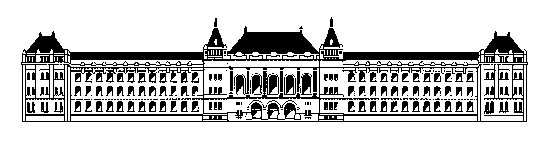
\includegraphics[width=3.648in, height=0.990in]{figures/usmanFig1}
%%\end{center}
%% %%\end{figure}

%% the following {center} is a trick -- vspace does nothing if there's
%% nothing above it in the page
\begin{center}\end{center}
\vspace{16em}
\hrule
\vspace{2em}
\begin{center}
\tbf{{\huge {\opp}}}\\
\vspace{1.5em}
{\LARGE Discrete Event Simulation System}\\
\vspace{1em}
{\large Version {\oppversion}}\\
\vspace{1em}
\tbf{\textit{{\LARGE User Manual}}}
\end{center}
\vspace{2em}
\hrule

%\vspace{4em}
%by {\large Andr\'{a}s Varga}
%\vspace{3em}

\vspace{8em}

%%\begin{center}
%%\textit{WORK IN PROGRESS}
%%\textit{Last updated: Oct 14, 2008}
%%\end{center}



%%% Local Variables:
%%% mode: latex
%%% TeX-master: "usman"
%%% End:

\cleardoublepage

%%\thispagestyle{empty}
\pagestyle{fancy}
\chapter*{Document History}


\begin{longtable}{|l|p{1cm}|p{10cm}|}
\hline
\tabheadcol
\tbf{Date} & \tbf{Author} & \tbf{Change}\\\hline
%%
2005/10 & AV & updated for the {\opp} 3.2 release\\\hline
%%
2005/03 & AV & updated for the {\opp} 3.1 release\\\hline
%%
2004/12 & AV & updated for the {\opp} 3.0 release\\\hline
%%
2003/06 & AV & Mentioned Grace and ROOT in section "Visualizing...".
               Added section "Using STL in message classes".
               \\\hline
%%
2003/06 & AV & OMNeT++ 2.3 released\\\hline
%%
2003/04-06 & AV & "Design of OMNeT++" chapter revised, extended, and renamed to
               "Customization and Embedding".
               Added "Interpreting Cmdenv output" section to the
               "Running the Simulation" chapter. Added section about Akaroa
               in "Running the Simulation" chapter. Expanded section about
               writing shell scripts to control the simulation.
               Added background info about RNGs and warning about old RNG
               in "Class Library" chapter;
               revised/extended "Deriving new classes" section in same chapter.
               Bibliography converted to Bibtex, expanded and cleaned up;
               citations added to text.
               "Parallel Simulation" chapter: contents removed until new PDES
               implementation gets released.
               Revised and reorganized NED chapter. Section about message
               sending/receiving and other simple module related functions
               moved to chapter "Simple Modules"; cMessage treatment from
               "Simulation Library" merged with message subclassing chapter
               into new chapter "Messages". Deprecated cPacket.
               Removed sections "Simulation techniques" and
               "Coding conventions", and their useful fragments were incorporated
               elsewhere. Added/created sections about message transmission
               modeling, and using global variables. Added sections explaining
               how to implement broadcasts and retransmissions. Revised section
               about dynamic module creation. Deprecated putaside-queue,
               receiveNew(), receiveOn().
               Added section "Object ownership management"; removed section
               on "Using shared objects". \\\hline
%%
2003/03 & AV & OMNeT++ 2.3b2 released\\\hline
%%
2003/02 & AV & OMNeT++ 2.3b1 released\\\hline
%%
2003/01 & AV & Added chapter about message subclassing; revised chapter about
               running the simulation and incorporated new Cmdenv options; added new
               distributions and clarified many details in NED expr. handling section\\\hline
%%
Summer 2002 & Ulrich Kaage & Converted from Word to LaTeX\\\hline
%%
2002/03/18 & AV & Documented new ini file options about Envir plugins\\\hline
%%
2002/01/24 & AV & Refinements on the Parsec chapter\\\hline
%%
2001/10/23 & AV & Updated to reflect changes since 2.1 release (see include/ChangeLog)\\\hline
%%
\end{longtable}




%%% Local Variables:
%%% mode: latex
%%% TeX-master: "usman"
%%% End:

\cleardoublepage

%%\setcounter{page}{1}
%\newpage
%%\pagenumbering{roman}
\tableofcontents
\cleardoublepage

%%\pagestyle{fancy}
\pagenumbering{arabic}

\chapter{Introduction}
\label{cha:introduction}


\section{What is {\opp}?}

{\opp} is an object-oriented modular discrete event network simulator.
The simulator can be used for:

\begin{itemize}
  \item{traffic modeling of telecommunication networks}
  \item{protocol modeling}
  \item{modeling queueing networks}
  \item{modeling multiprocessors and other distributed hardware systems}
  \item{validating hardware architectures}
  \item{evaluating performance aspects of complex software systems}
  \item{\dots modeling any other system where the discrete event approach is
    suitable.}
\end{itemize}


An {\opp} model consists of hierarchically nested modules. The
depth of module nesting is not limited, which allows the user
to reflect the logical structure of the actual system in the
model structure. Modules communicate through message passing. Messages
can contain arbitrarily complex data structures. Modules can
send messages either directly to their destination or along a
predefined path, through gates and connections.


Modules can have their own parameters. Parameters can be used to customize
module behaviour and to parameterize the model's topology.

Modules at the lowest level of the module hierarchy encapsulate
behaviour. These modules are termed simple modules, and they are
programmed in C++ using the simulation library.

{\opp} simulations can feature varying user interfaces for
different purposes: debugging, demonstration and batch execution.
Advanced user interfaces make the inside of the model visible
to the user, allow control over simulation execution
and to intervene by changing variables/objects inside the model.
This is very useful in the development/debugging phase
of the simulation project. User interfaces also facilitate demonstration
of how a model works.

The simulator as well as user interfaces and tools are portable:
they are known to work on Windows and on several Unix flavours,
using various C++ compilers.

{\opp} also supports parallel distributed simulation. {\opp} can
use several mechanisms for communication between partitions of
a parallel distributed simulation, for example MPI or named pipes.
The parallel simulation algorithm can easily be extended or new
ones plugged in. Models do not need any special instrumentation
to be run in parallel -- it is just a matter of configuration.
{\opp} can even be used for classroom presentation of parallel
simulation algorithms, because simulations can be run in parallel
even under the GUI which provides detailed feedback on what is going on.

{\omnest} is the commercially supported version of {\omnetpp}.
{\omnetpp} is only free for academic and non-profit use --
for commercial purposes one needs to obtain {\omnest} licenses
from Omnest Global, Inc.


% \section{Where does {\opp} stand in the world of simulation tools?}
%
% There are numerous network simulation tools on the market today,
% both commercial and non-commercial. In this section I will try
% to give an overview by picking some of the most important or
% most representative ones in both categories and comparing them
% to {\opp}: PARSEC, SMURPH, NS, Ptolemy, NetSim++, C++SIM, CLASS
% as non-commercial, and OPNET, COMNET III as commercial tools.
% (The {\opp} Home Page contains a list of Web sites with collections
% of references to network simulation tools where the reader can
% get a more complete list.) In the commercial category, OPNET
% is widely held to be the state of the art in network simulation.
% {\opp} is targeted at roughly the same segment of network simulation
% as OPNET.
%
% Seven issues are examined to get an overview about the network
% simulation tools:
%
%
% \textbf{Detail Level}. \textit{Does the simulation tool have the necessary
% power to express details in the model?} In other words, can the
% user implement arbitrary new building blocks like in {\opp}
% or he is confined to the predefined blocks implemented by the
% supplier? Some tools like COMNET III are not programmable by
% the user to this extent therefore they cannot be compared to
% {\opp}. Specialized network simulation tools like NS (for IP)
% and CLASS (for ATM) also rather fall into this category.
%
%
% \textbf{Available Models.} \textit{What protocol models are readily available
% for the simulation tool?} As of end 2004, there are three large
% protocol modelling frameworks available for {\opp}:
% the Mobility Framework for modelling mobile, wireless and ad-hoc networks;
% the INET Framework with TCP, IP, MPLS and other Internet-related protocols;
% and IPv6Suite which provides detailed models for IPv6, Mobile IPv6, 802.11
% and other protocols. Several other simulation models (such as AntNet routing)
% have also been published -- the list is ever growing, and model frameworks
% are constantly maturing and converging.
%
%
% \textbf{Defining Network Topology}. \textit{How does the simulation
% tool support defining the network topology?} Is it possible to
% create some form of hierarchy (nesting) or only ``flat'' topologies
% are supported? Network simulation tools naturally share the property
% that a model (network) consists of ``nodes'' (blocks, entities,
% modules, etc.) connected by ``links'' (channels, connections, etc.).
% Many commercial simulators have graphical editors to define the
% network; however, this is only a good solution if there is an
% alternative form of topology description (e.g. text file) which allows
% one to generate the topology by program. OPNET follows a unique way:
% the network topology is stored in a proprietary binary file format
% which can be generated (and read) by the graphical editor and C
% programs linked against a special library. On the other hand, most
% non-commercial simulation tools do not provide explicit support for
% topology description: one must program a ``driver entity'' which will
% boot the model by creating the necessary nodes and interconnecting
% them (PARSEC, SMURPH, NS). Finally, a large part of the tools that do
% support explicit topology description supports only flat topologies
% (CLASS). {\opp} probably uses the most flexible method: it has a
% human-readable textual topology description format (the NED language)
% which is easy to create with any text-processing tool (\fprog{perl},
% \fprog{awk}, etc.), and the same format is used by the graphical
% editor. It is also possible to create a ``driver entity'' to build a
% network at run-time by program. {\opp} also supports submodule
% nesting.
%
%
% \textbf{Programming Model.} \textit{What is the programming model supported
% by the simulation environment?} Network simulators typically use
% either thread/coroutine-based programming (such as \fname{activity()}
% in {\opp}), or FSMs built upon a \fname{handleMessage()}-like function.
% For example, OPNET, SMURPH and NetSim++ use FSMs (with underlying
% handleMessage()), PARSEC and C++SIM use threads. {\opp} supports
% both programming models; the author does not know of another
% simulation tool that does so.
%
%
% \textbf{Debugging and Tracing Support.} \textit{What debugging or tracing
% facilities does the simulation tool offer?} Simulation programs
% are infamous for long debugging periods. C++-based simulation
% tools rarely offer much more than \fname{printf()}-style debugging; often
% the simulation kernel is also capable of dumping selected debug
% information on the standard output. Animation is also often supported,
% either off-line (record\&playback) or in some client-server architecture,
% where the simulation program is the ``server'' and
% it can be viewed using the ``client''. Off-line animation
% naturally lacks interactivity and is therefore little use in
% debugging. The client-server solution typically has limited power
% because the simulation and the viewer run as independent operating
% system processes, and the viewer has limited access to the simulation
% program's internals and/or it does not have enough control over
% the course of simulation execution. OPNET has a very good support
% for command-line debugging and provides both off-line and client-server
% style animation. NetSim++ and Ptolemy use the client-server method
% of animation. {\opp} goes a different way by linking the GUI
% library with the debugging/tracing capability into the simulation
% executable. This architecture enables the GUI to be very powerful:
% every user-created object is visible (and modifiable) in the
% GUI via inspector windows and the user has tight control over
% the execution. To the author's best knowledge, the tracing feature
% {\opp} provides is unique among the C++-based simulation tools.
%
%
% \textbf{Performance.} \textit{What performance can be expected from the
% simulation?} Simulation programs typically run for several hours.
% Probably the most important factor is the programming language;
% almost all network simulation tools are C/C++-based. Performance
% is a particularly interesting issue with {\opp} since the GUI
% debugging/tracing support involves some extra overhead in the
% simulation library. However, in a reported case, an {\opp} simulation
% was only 1.3 slower than its counterpart implemented in plain
% C (i.e. one containing very little administration overhead),
% which is a very good showing. A similar result was reported in
% a performance comparison with a PARSEC simulation.
%
%
% \textbf{Source Availability.} \textit{Is the simulation library available
% in source?} This is a trivial question but it immediately becomes
% important if one wants to examine or teach the internal workings
% of a simulation kernel, or one runs into trouble because some
% function in the simulation library has a bug and/or it is not
% documented well enough. In general it can be said that non-commercial
% tools (like {\opp}) are open-source and commercial ones are
% not. This is also true for OPNET: the source for simulation kernel
% is not available (although the ready-made protocol models come
% with sources).
%
%
% In conclusion, it can be said that {\opp} has enough features
% to make it a good alternative to most network simulation tools,
% and it has a strong potential to become one of the most widely
% used network simulation packages in academic and research environments.
%

\section{Organization of this manual}

The manual is organized the following way:

\begin{itemize}
  \item{The chapters \ref{cha:introduction} and \ref{cha:overview}
    contain introductory material}
  \item{The second group of chapters,
    \ref{cha:the-ned-language},
    \ref{cha:simple-modules} and
    \ref{cha:the-simulation-library}
    are the programming guide. They present the NED language\index{ned!language},
    the simulation concepts and their implementation in {\opp}, explain
    how to write simple\index{module!simple} modules and describe the class library.}
  \item{The chapters
    \ref{cha:graphics} and
    \ref{cha:neddoc}
    elaborate the topic further, by explaining how one can customize
    the network graphics and how to write NED source code comments
    from which documentation can be generated.}
  \item{The following chapters,
    \ref{cha:building-simulation-programs},
    \ref{cha:run-sim} and
    \ref{cha:analyzing-simulation-results} deal with practical issues
    like building and running simulations and analyzing results, and
    present the tools {\opp} provides to support these tasks.}
  \item{Chapter \ref{cha:parallel-execution} is devoted to the support
    of distributed execution.}
  \item{Finally, Chapter \ref{cha:opp-design} explains the
    architecture and the internals of {\opp}. This chapter will be
    useful to those who want to extend the capabilities of the
    simulator or want to embed it into a larger application.}
%  \item{The first two Appendices, \ref{cha:opnet-and-omnet} and
%    \ref{cha:parsec-and-omnet}, contain a comparison of {\opp} and
%    two other important and well-known simulation tools, OPNET and
%    PARSEC.}
  \item{Appendix \ref{cha:ned-language-grammar} provides a reference
    of the NED language\index{ned!language}.}
\end{itemize}




% \section{History}
%
% \tbf{The early days: 1992-1997}
%
% {\omnetpp} has its distant roots in OMNeT, a simulator written
% in Object Pascal by dr. Gy\"{o}rgy Pongor.
% The development of {\omnetpp} started as a semester's programming
% assignment at the Technical University of Budapest (BME) in 1992.
% The assignment (``creation of an object-oriented discrete event
% simulation system in C++'') was handed out by Prof. Dr Gy\"{o}rgy
% Pongor, and two students signed up: \'{A}kos Kun and Andr\'{a}s Varga.
% The basis for the design was Mr. Pongor's existing simulation
% software written in Pascal, named OMNeT.
%
% We started developing the code in Borland C++ 3.1. The idea
% of multiple runtime environments, a significant addition to the
% original OMNeT design, was there from the very beginning.
% We used Turbo Vision (Borland's then successful character-based
% GUI) for the first `graphical' user interface.
%
% In 1992, we submitted a paper about {\omnetpp} to the
% student's annual university conference
% (named ``TDK'') and won first prize in the ``Software'' section.
% Later we also won 1st prize in the national ``TDK''. Then the
% idea came to port {\omnetpp} to Unix (first for AIX on an RS/6000
% with only 16MB RAM, later Linux), until all development was done
% in Linux and BC3.1 could no longer be supported.
%
% Well, here's a brief list of events since then -- maybe one time
% I'll make up my mind to enhance them to a whole story\dots
%
% 1994: XEnv (a GUI in pure MOTIF, superceded by Tkenv by now)
% was written as diploma work
%
% 1994: used OPNET for several simulation projects. OPNET features
% (and flaws) gave lots of ideas how to continue with {\omnetpp}.
%
% 1995: initial version of nedc was written by a group of exchange
% students from Delft
%
% 1996: initial version of PVM support was programmed by Zoltan
% Vass as diploma work
%
% 1997: started working on Tkenv
%
% 1997 Dec: added GNED
%
% \tbf{Regular open-source releases: 1997-2003}
%
% Until 1997, some people occasionally contributed to {\omnetpp}.
% Since 1997, all development is done entirely by Andras;
% independent of the University since 1998. (He leaves
% the University in 1998, and is no longer affiliated with it
% since then.)
%
% 1997 Sept: web site set up (www.hit.bme.hu/phd/vargaa/omnetpp), first public release
%
% 1997 Feb-1998 Sept: simulation projects for a small company in
% Hungary. We used a version of {\omnetpp}.
%
% 1998 March: added Plove
%
% 1998 June: animation implemented in Tkenv
%
% 1998 Sept-1999 May: work at MeTechnology (later Brokat) in Leipzig
%
% 2000 Jan: MSVC porting
%
% 2000 Sept: contributed model repository set up
%
% 2000: IPSuite created in Karlsruhe
%
% 2001 May: {\omnetpp} 2.1 release
%
% 2001 June: the CVS gets hosted in Karlsruhe
%
% 2002 May: {\omnetpp} 2.2 release
%
% 2003 Jan: Omnest Global Inc. was founded
%
% 2003 Feb-Oct: Andras's stay at CTIE, Monash University, Melbourne, Australia
% with Ahmet Sekercioglu's group; development of {\omnetpp}'s parallel simulation
% framework, doing parallel simulation experiments
%
% 2003 June: first public release of IPv6Suite (CTIE, Monash University)
%
% 2003 July: launch of www.omnetpp.org
%
% 2003 July: release of RSVP/TE models at UTS Sydney
%
% 2003 Aug: Andras takes over IPSuite maintenance
%
% 2003 Sept: Ethernet model made available
%
% 2003 Nov: {\omnetpp} 2.3p1 release
%
% 2004 July: Mobility Framework first official release (TKN, TU Berlin)
%
% 2004 Oct: IPSuite renamed to INET Framework
%
% \dots
%


\section{Credits}

{\omnetpp} has been developed by Andr\'{a}s Varga (andras@omnetpp.org,
andras.varga@omnest.com).

In the early stage of the project, several people have contributed
to {\omnetpp}. Although most contributed code is no longer part of
the {\omnetpp}, nevertheless I'd like to acknowledge the work of the
following people. First of all, I'd like thank Dr Gy\"{o}rgy Pongor
(pongor@hit.bme.hu), my advisor at the Technical University of Budapest
who initiated the {\omnetpp} as a student project.

My fellow student \'{A}kos Kun started to program the first NED parser
in 1992-93, but it was abandoned after a few months.
The first version of nedc was finally developed in summer 1995,
by three exchange students from TU Delft: Jan Heijmans, Alex Paalvast
and Robert van der Leij. nedc was first called JAR after their initials
until it got renamed to nedc. nedc was further developed and refactored
several times until it finally retired and got replaced by nedtool in {\omnetpp} 3.0.
The second group of Delft exchange students (Maurits Andr\'{e},
George van Montfort, Gerard van de Weerd) arrived in fall 1995.
They performed some testing of the simulation library, and
wrote some example simulations, for example the original version of Token Ring,
and simulation of the NIM game which survived until {\omnetpp} 3.0.
These student exchanges were organized by Dr. Leon Rothkranz
at TU Delft, and Gy\"{o}rgy Pongor at TU Budapest.

The diploma thesis of Zolt\'{a}n Vass (spring 1996) was to prepare
{\omnetpp} for parallel execution over PVM to {\omnetpp}. This code has been
replaced with the new Parallel Simulation Architecture in {\omnetpp} 3.0.
G\'{a}bor Lencse (lencse@hit.bme.hu) was also interested in parallel
simulation, namely a method called Statistical Synchronization (SSM).
He implemented the FDDI model (practically unchanged until now), and added
some extensions into NED for SSM. These extensions have been removed
since then ({\omnetpp} 3.0 does parallel execution on different principles).

The $P^{2}$ algorithm and the original implementation of the k-split algorithm
was programmed in fall 1996 by Babak Fakhamzadeh from TU Delft.
k-split was later reimplemented by Andr\'{a}s.

Several bugfixes and valuable suggestions for improvements came
from the user community of {\omnetpp}. It would be impossible to
mention everyone here, and the list is constantly growing --
instead, the README and ChangeLog files contain acknowledgements.

Between summer 2001 and fall 2004, the {\omnetpp} CVS was hosted
at the University of Karlsruhe. Credit for setting
up and maintaining the CVS server goes to Ulrich Kaage.
Ulrich can also be credited with converting the User Manual from
Microsoft Word format to LaTeX, which was a huge undertaking
and great help.


%%% Local Variables:
%%% mode: latex
%%% TeX-master: "usman"
%%% End:

\cleardoublepage

\chapter{Overview}
\label{cha:overview}


\section{Modeling concepts}

An {\opp} model consists of modules that communicate with message passing.
The active modules are termed \textit{simple modules}; they are written in C++,
using the simulation class library. Simple modules can be grouped into
\textit{compound modules} and so forth; the number of hierarchy levels is not
limited. Messages can be sent either via connections that span between
modules or directly to their destination modules. The concept of simple and
compound modules is similar to DEVS atomic and coupled models.
%TODO add ref to DEVS papers

Both simple and compound modules are instances of \textit{module types}.
When describing the model, the user defines module types; instances of these
module types serve as components for more complex module types. Finally,
the user creates the system module as a network module which is a special
compound module type without gates to the external world. When a module
type is used as a building block, there is no distinction whether it is a
simple or a compound module. This allows the user to transparently split a
module into several simple modules within a compound module, or do the
opposite, re-implement the functionality of a compound module in one simple
module, without affecting existing users of the module type.

In Fig. \ref{fig:ch-overview:modules}, boxes represent simple modules
(thick border) and compound modules (thin border).
Arrows connecting small boxes represent connections and gates.

\begin{figure}[htbp]
\begin{center}
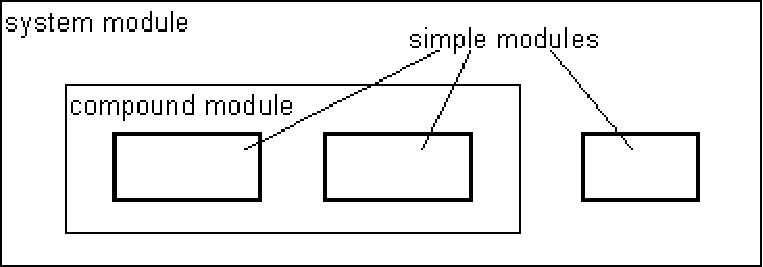
\includegraphics[width=3.772in, height=1.292in]{figures/usmanFig2}
\caption{Simple and compound modules}
\label{fig:ch-overview:modules}
\end{center}
\end{figure}


Modules communicate with messages which -- in addition to
usual attributes such as timestamp -- may contain arbitrary
data. Simple modules typically send messages via gates, but it is also
possible to send them directly to their destination modules. Gates are the
input and output interfaces of modules: messages are sent out through
output gates and arrive through input gates. An input and an output gate
can be linked with a connection. Connections are created within a single
level of module hierarchy: within a compound module, corresponding gates of
two submodules, or a gate of one submodule and a gate of the compound
module can be connected. Connections spanning across hierarchy levels are
not permitted, as it would hinder model reuse. Due to the hierarchical
structure of the model, messages typically travel through a chain of
connections, to start and arrive in simple modules. Compound modules act as
'cardboard boxes' in the model, transparently relaying messages between
their inside and the outside world. Properties such as propagation delay,
data rate and bit error rate, can be assigned to connections. One can also
define connection types with specific properties (termed channels) and
reuse them in several places. Modules can have parameters. Parameters are
mainly used to pass configuration data to simple modules, and to help
define model topology. Parameters may take string, numeric or boolean
values. Because parameters are represented as objects in the program,
parameters -- in addition to holding constants -- may transparently act as
sources of random numbers with the actual distributions provided with the
model configuration, they may interactively prompt the user for the value,
and they might also hold expressions referencing other parameters. Compound
modules may pass parameters or expressions of parameters to their
submodules.






{\opp} provides efficient tools for the user to describe the
structure of the actual system. Some of the main features are:
\begin{itemize}
\item{hierarchically nested modules}
\item{modules are instances of module types}
\item{modules communicate with messages through channels}
\item{flexible module parameters}
\item{topology description language}
\end{itemize}

\subsection{Hierarchical modules}


An {\opp} model consists of hierarchically nested
modules\index{module!hierarchy}, which communicate by passing
messages to each another.
{\opp} models are often referred to as \textit{networks}. The top
level module is the \textit{system module}.  The system module
contains \textit{submodules}, which can also contain submodules
themselves (Fig. \ref{fig:ch-overview:modules}). The depth of module
nesting is not limited; this allows the user to reflect the logical
structure of the actual system in the model structure.

Model structure is described in {\opp}'s NED language.

\begin{figure}[htbp]
\begin{center}
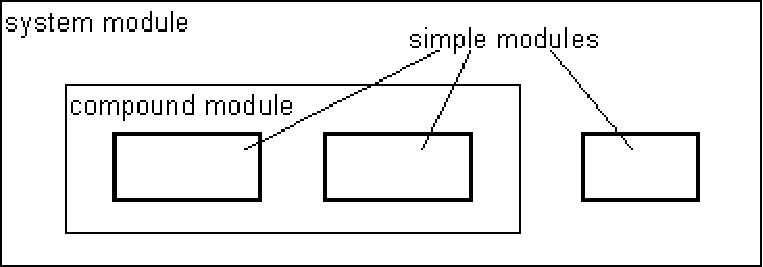
\includegraphics[width=3.772in, height=1.292in]{figures/usmanFig2}
\caption{Simple and compound modules}
\label{fig:ch-overview:modules}
\end{center}
\end{figure}


Modules that contain submodules are termed \textit{compound
  modules}\index{module!compound}, as opposed \textit{simple
  modules}\index{module!simple} which are at the lowest level of the
module hierarchy. Simple modules contain the algorithms in the model.
The user implements the simple modules in C++, using the {\opp}
simulation class library.


\subsection{Module types}
\index{module!types}

Both simple and compound modules are instances of \textit{module
  types}. While describing the model, the user defines module types;
instances of these module types serve as components for more complex
module types. Finally, the user creates the system module as an
instance of a previously defined module type; all modules of the
network are instantiated as submodules and sub-submodules of the
system module.

When a module type is used as a building block, there is no
distinction whether it is a simple or a compound module. This allows
the user to split a simple module into several
simple modules embedded into a compound\index{module!compound} module,
or vica versa, aggregate the functionality of a compound module into a
single simple module, without affecting existing users of the module
type.

Module types can be stored in files separately from the place
of their actual usage. This means that the user can group existing
module types and create \textit{component libraries}\index{module!libraries}. This feature
will be discussed later, in Chapter \ref{cha:run-sim}.



\subsection{Messages, gates, links}

Modules communicate by exchanging
\textit{messages}\index{message!exchanging}. In an actual simulation,
messages can represent frames or packets in a computer network, jobs
or customers in a queuing network or other types of mobile entities.
Messages can contain arbitrarily complex data structures. Simple
modules can send messages either directly to their destination or
along a predefined path, through gates and connections.


The ``local simulation time'' of a module advances when the module
receives a message. The message can arrive from another module
or from the same module (\textit{self-messages} are used to implement
timers).


\textit{Gates}\index{gate} are the input and output interfaces of
modules; messages are sent out through output gates and arrive through
input gates.

Each \textit{connection}\index{connection} (also called
\textit{link}\index{link}) is created within a single level of the
module hierarchy: within a compound module, one can connect the
corresponding gates of two submodules, or a gate of one submodule and
a gate of the compound module (Fig.
\ref{fig:ch-overview:connections}).

\begin{figure}[htbp]
\begin{center}
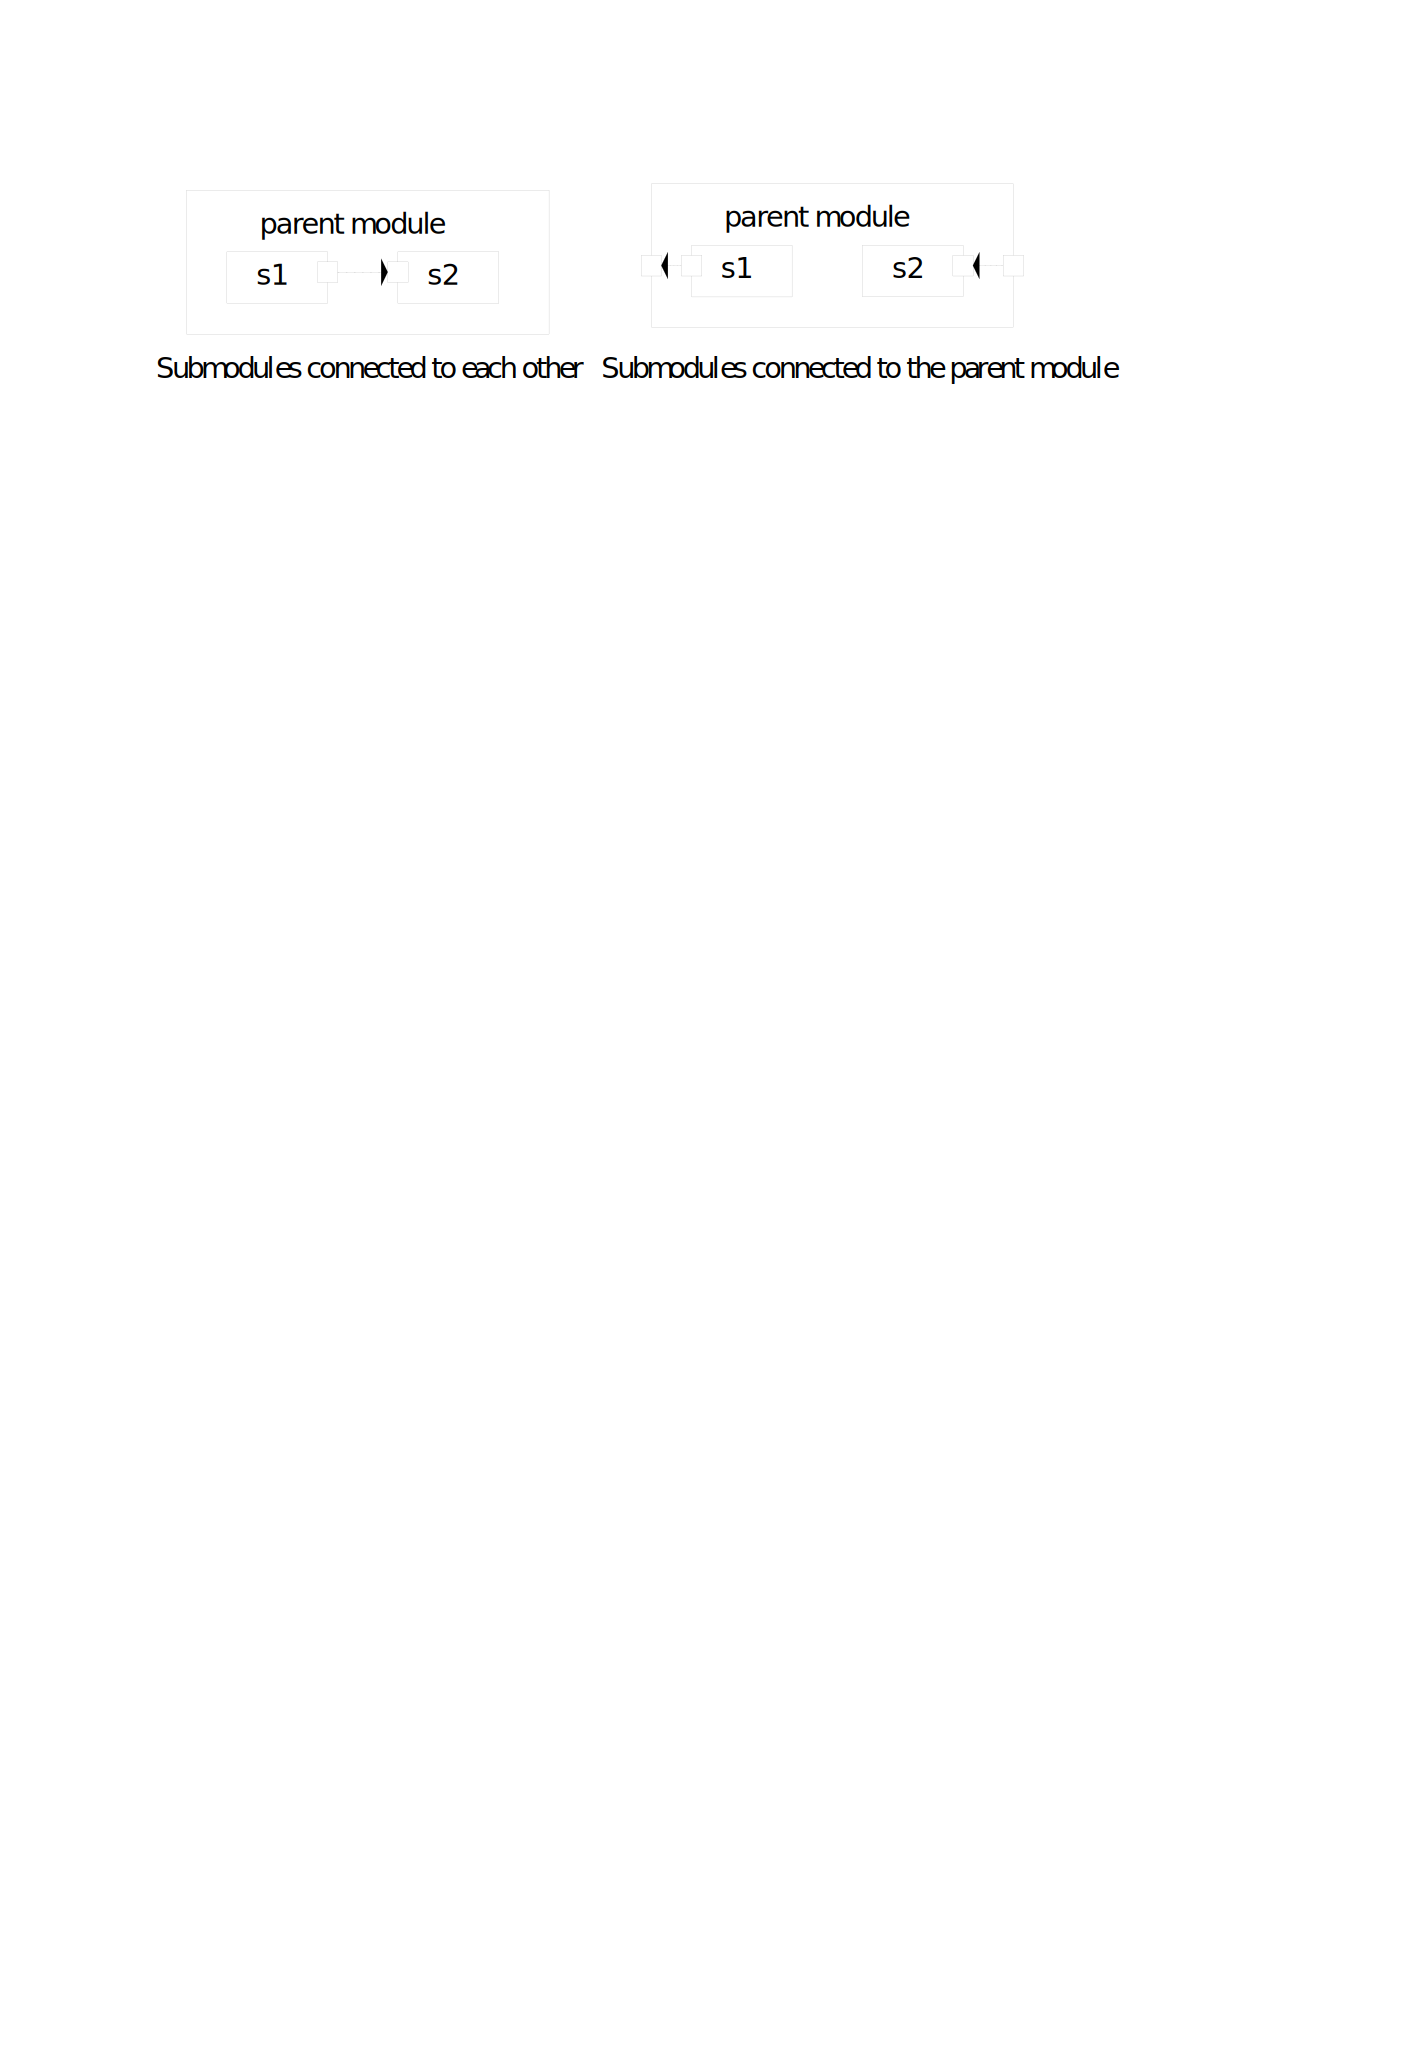
\includegraphics[width=5.061in, height=1.121in]{figures/usmanFig3}
\caption{Connections}
\label{fig:ch-overview:connections}
\end{center}
\end{figure}

Due to the hierarchical structure of the model, messages typically
travel through a series of connections, to start and arrive in simple
modules. Such series of connections that go from simple module to
simple module are called \textit{routes}.  Compound modules act as
`cardboard boxes' in the model, transparently relaying messages
between their inside and the outside world.


\subsection{Modeling of packet transmissions}

Connections can be assigned three parameters, which facilitate
the modeling of communication networks, but can be useful in
other models too: \textit{propagation delay}, \textit{bit error rate}
and \textit{data rate}, all three being optional. One can specify
link parameters individually for each connection, or define link types
and use them throughout the whole model.

Propagation delay is the amount of time the arrival of
the message is delayed by when it travels through the channel.

Bit error rate speficifies the probability that a bit is incorrectly
transmitted, and allows for simple noisy channel modelling.

Data rate is specified in bits/second, and it is used for calculating
transmission time of a packet.

When data rates are in use, the sending of the message in the model
corresponds to the transmission of the first bit, and
the arrival of the message corresponds to the reception
of the last bit. This model is not always applicable,
for example protocols like Token Ring and FDDI do not wait
for the frame to arrive in its entirety, but rather start repeating
its first bits soon after they arrive -- in other words,
frames ``flow through'' the stations, being delayed only a few bits.
If you want to model such networks, the data rate modeling feature
of {\opp} cannot be used.



\subsection{Parameters}
\index{module!parameters}
\index{parameters|see{module parameters}}

Modules can have parameters. Parameters can be assigned either
in the NED files or the configuration file omnetpp.ini.

Parameters may be used to customize simple module behaviour,
and for parameterizing the model topology.

Parameters can take string, numeric or boolean values, or can
contain XML data trees. Numeric values include expressions using
other parameters and calling C functions, random variables from
different distributions, and values input interactively by the user.

Numeric-valued parameters can be used to construct topologies in a
flexible way. Within a compound module, parameters can define the
number of submodules, number of gates, and the way the internal
connections are made.


\subsection{Topology description method}
\index{topology!description}
The user defines the structure of the model in NED language descriptions
(Network Description).The NED language will be discussed in detail
in Chapter \ref{cha:the-ned-language}.


\section{Programming the algorithms}

The simple\index{module!simple} modules of a model contain algorithms
as C++ functions.
The full flexibility and power of the programming language can
be used, supported by the {\opp} simulation class library.
The simulation programmer can choose between event-driven and process-style
description, and can freely use object-oriented concepts
(inheritance, polymorphism etc) and design patterns to extend the
functionality of the simulator.

Simulation objects (messages, modules, queues etc.) are represented
by C++ classes. They have been designed to work together efficiently,
creating a powerful simulation programming framework.
The following classes are part of the simulation class library:

\begin{itemize}
  \item{modules, gates, connections etc.}
  \item{parameters}
  \item{messages}
  \item{container classes (e.g. queue, array)}
  \item{data collection classes}
  \item{statistic and distribution estimation classes (histograms, $P^2$
  algorithm for calculating quantiles etc.)}
  \item{transient detection and result accuracy detection classes}
\end{itemize}

The classes are also specially instrumented, allowing one
to traverse objects of a running simulation and display information
about them such as name, class name, state variables or contents.
This feature has made it possible to create a simulation GUI where
all internals of the simulation are visible.


% \subsection{Creating simple modules}
% \index{module!simple!creation}
%
% Each simple\index{module!simple} module type is implemented with a C++ class. Simple
% module classes are derived from a simple module base class, by
% redefining the virtual function that contains the algorithm.
% The user can add other member functions to the class to split
% up a complex algorithm; he can also add data members to the class.
%
% It is also possible to derive new simple\index{module!simple} module classes from
% existing ones. For example, if one wants to experiment with retransmission
% timeout schemes in a transport protocol, he can implement the
% protocol in one class, create a virtual function for the retransmission
% algorithm and then derive a family of classes that implement
% concrete schemes. This concept is further supported by the fact
% that in the network description, actual module types can be parameters.
%
%
% \subsection{Object mechanisms}
%
% The use of smart container classes allows the user to build
% \textit{aggregate data structures}\index{aggregate data structures}.
% For example, one can add any number of objects to a message object as
% parameters. Since the added objects can contain further objects,
% complex data structures can be built.
%
% There is an efficient \textit{ownership}\index{ownership} mechanism
% built in. The user can specify an owner for each object; then, the
% owner object will have the responsibility of destroying that object.
% Most of the time, the ownership mechanism works transparently;
% ownership only needs to be explicitly managed when the user wants to
% do something non-typical.
%
%
% The \textit{foreach}\index{forEachChild mechanism} mechanism allows one to
% enumerate the objects inside a container object in a uniform way and
% do some operation on them. This feature which makes it possible to
% handle many objects together. (The \textit{foreach} feature is extensively used
% by the user interfaces with debugging capability and the snapshot
% mechanism; see later.)
%
%
% \subsection{Derive new classes}
%
% It most cases, the functionality offered by the {\opp} classes
% is enough for the user. But if it is needed, one can derive new
% classes from the existing ones or create entirely new classes.
% For flexibility, several member functions are declared virtual.
% When the user creates new classes, certain rules need to be kept
% so that the object can fully work together with other objects.
%
%
% \subsection{Self-describing objects to ease debugging}
% \index{debugging}
%
%
%
% A unique feature called \textit{snapshot}\index{snapshot} allows the
% user to dump the contents of the simulation model or a part of it into
% a text file. The file will contain textual reports about every object;
% this can be of invaluable help at times of debugging. Ordinary
% variables can also be made to appear in the snapshot file. Snapshot
% creations can be scheduled from within the simulation program or done
% from the user interface.
%


\section{Using {\opp}}


\subsection{Building and running simulations}
\index{simulation!building}
\index{simulation!running}

This section provides insight into working with {\opp} in practice:
Issues such as model files, compiling and running simulations are
discussed.

An {\opp} model consists of the following parts:
\begin{itemize}
  \item{NED language topology description(s)\index{ned!files} (\texttt{.ned} files)
    which describe the module structure with parameters, gates etc.
    NED files can be written using any text editor or the
    GNED graphical editor\index{ned!graphical editor}.}
  \item{Message definitions (\texttt{.msg} files). You can define various message
    types and add data fields to them. {\opp} will translate message definitions
    into full-fledged C++ classes.}
  \item{Simple modules sources. They are C++ files, with \texttt{.h}/\texttt{.cc} suffix.}
\end{itemize}

The simulation system provides the following components:
\begin{itemize}
  \item{Simulation kernel\index{simulation!kernel}. This contains the
    code that manages the simulation and the simulation class library.
    It is written in C++, compiled and put together to form a library
    (a file with .a or .lib extension)}
  \item{User interfaces\index{simulation!user interface}.
    \index{user interface} {\opp} user interfaces
    are used in simulation execution, to facilitate debugging,
    demonstration, or batch execution of simulations. There are
    several user interfaces, written in C++, compiled and put together
    into libraries (\texttt{.a} or \texttt{.lib} files).}
\end{itemize}


Simulation programs are built from the above components. First,
\ttt{.msg} files are translated into C++ code using the \ttt{opp\_msgc}.
program. Then all C++ sources are compiled, and linked with the simulation
kernel and a user interface library to form a simulation executable.
NED files\index{ned!files} can either be also translated into C++
(using \ttt{nedtool}) and linked in, or loaded dynamically in their original
text forms when the simulation program starts.



\subsubsection{Running the simulation and analyzing the results}

The simulation executable is a standalone program,
thus it can be run on other machines without {\opp} or the model files
being present. When the program is started, it reads a configuration
file\index{simulation!configuration file} (usually called
\texttt{omnetpp.ini}\index{omnetpp.ini}). This file contains settings that
control how the simulation is executed, values for model parameters, etc.
The configuration file can also prescribe several simulation runs; in
the simplest case, they will be executed by the simulation program one
after another.

The output of the simulation is written into data files: output vector
files\index{output!vector file}, output scalar files
\index{output!scalar file}, and possibly the user's own output files.
{\opp} provides a GUI tool named Plove to view and plot the contents
of output vector files. It is not expected that someone will
process the result files using {\opp} alone: output files are text
files in a format which can be read into math packages like Matlab
or Octave, or imported into spreadsheets like OpenOffice Calc,
Gnumeric or MS Excel (some preprocessing using \fprog{sed}, \fprog{awk}
or \fprog{perl} might be required, this will be discussed later).
All these external programs provide rich functionality for statistical
analysis and visualization, and it is outside the scope of {\opp} to
duplicate their efforts. This manual briefly describes
some data plotting programs and how to use them with {\opp}.

Output scalar files can be visualized using the Scalars tool.
It can draw bar charts, x-y plots (e.g. throughput vs offered load),
or export data via the clipboard for more detailed analysis into
spreadsheets and other programs.


\subsubsection{User interfaces}
\index{simulation!user interface}

The primary purpose of user interfaces is to make the internals
of the model visible to the user, to control simulation execution,
and possibly allow the user to intervene by changing variables/objects
inside the model. This is very important in the development/debugging
phase of the simulation project. Just as important, a hands-on
experience allows the user to get a `feel' of the model's
behaviour. The graphical user interface can also be used to
demonstrate a model's operation.


The same simulation model can be executed with different user
interfaces, without any change in the model files themselves.
The user would test and debug the simulation with a powerful
graphical user interface, and finally run it with a simple and
fast user interface that supports batch execution.


\subsubsection{Component libraries}
\index{module!libraries}

Module types can be stored in files separate from the place
of their actual use. This enables the user to group existing
module types and create component libraries.


\subsubsection{Universal standalone simulation programs}


A simulation executable can store several independent models
that use the same set of simple modules. The user can specify
in the configuration file which model is to be run. This
allows one to build one large executable that contains several
simulation models, and distribute it as a standalone simulation
tool. The flexibility of the topology description language also
supports this approach.


\subsection{What is in the distribution}

If you installed the source distribution, the omnetpp directory on your system
should contain the following subdirectories. (If you installed a precompiled
distribution, some of the directories may be missing, or there might be
additional directories, e.g. containing software bundled with {\opp}.)

The simulation system itself:

\begin{Verbatim}[commandchars=\\\{\}]
  \tbf{omnetpp/}         {\opp} root directory
    \tbf{bin/}           {\opp} executables (GNED, nedtool, etc.)
    \tbf{include/}       header files for simulation models
    \tbf{lib/}           library files
    \tbf{bitmaps/}       icons that can be used in network graphics
    \tbf{doc/}           manual (PDF), readme, license, etc.
      \tbf{manual/}      manual in HTML
      \tbf{tictoc-tutorial/}  introduction into using {\opp}
      \tbf{api/}         API reference in HTML
      \tbf{nedxml-api/}  API reference for the NEDXML library
      \tbf{src/}         sources of the documentation
    \tbf{src/}           {\opp} sources
      \tbf{nedc/}        nedtool, message compiler
      \tbf{sim/}         simulation kernel
        \tbf{parsim/}    files for distributed execution
        \tbf{netbuilder/}files for dynamically reading NED files
      \tbf{envir/}       common code for user interfaces
      \tbf{cmdenv/}      command-line user interface
      \tbf{tkenv/}       Tcl/Tk-based user interface
      \tbf{gned/}        graphical NED editor
      \tbf{plove/}       output vector analyzer and plotting tool
      \tbf{scalars}      output scalar analyzer and plotting tool
      \tbf{nedxml/}      NEDXML library
      \tbf{utils/}       makefile-creator, documentation tool, etc.
    \tbf{test/}          regression test suite
      \tbf{core/}        regression test suite for the simulation library
      \tbf{distrib/}     regression test suite for built-in distributions
      ...
\end{Verbatim}

Sample simulations are in the \texttt{samples} directory.

\begin{Verbatim}[commandchars=\\\{\}]
    \tbf{samples/}     directories for sample simulations
      \tbf{aloha/}     models the Aloha protocol
      \tbf{cqn/}       Closed Queueing Network
      ...
\end{Verbatim}

The \texttt{contrib} directory contains material from the {\opp} community.

\begin{Verbatim}[commandchars=\\\{\}]
    \tbf{contrib/}     directory for contributed material
      \tbf{octave/}    Octave scripts for result processing
      \tbf{emacs/}     NED syntax highlight for Emacs
\end{Verbatim}

You may also find additional directories like \texttt{msvc/}, which contain
integration components for Microsoft Visual C++, etc.


%%% Local Variables:
%%% mode: latex
%%% TeX-master: "usman"
%%% End:

\cleardoublepage

\chapter{An Example: The NIM Game}
\label{cha:the-nim-game}


This chapter contains a full example program that can give you 
some basic idea of using the simulator. An enhanced version of 
the NIM example can be found among the sample programs.

Nim is an ancient game with two players and a bunch of sticks. 
The players take turns, removing 1, 2, 3 or 4 sticks from the 
heap of sticks at each turn. The one who takes the last stick 
is the loser. 


Of course, building a model of the Nim game is not much of a 
simulation project, but it nicely demonstrates the modeling approach 
used by {\opp}.


Describing the model consists of two phases:
\begin{itemize}
\item{topology description}
\item{defining the operation of components}
\end{itemize}



\section{Topology}

The game can be modelled in {\opp} as a network with three modules: 
the ''game'' (a manager module) and two players. 
The modules will communicate by exchanging messages. The ''game'' 
module keeps the current number of tokens and organizes the game; 
in each turn, the player modules receives the number of tokens 
from the Game module and sends back its move.

\begin{figure}[htbp]
\begin{center}
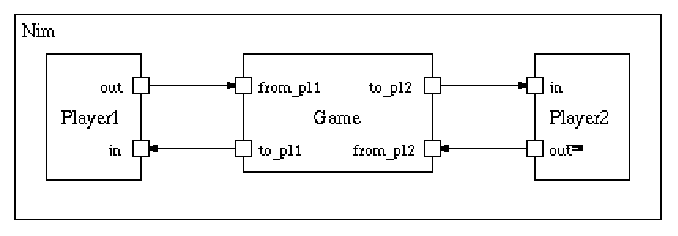
\includegraphics[width=4.483in, height=1.568in]{figures/usmanFig6}
\caption{Module structure for the Nim game.}
\end{center}
\end{figure}

\texttt{Player1}, \texttt{Player2} and \texttt{Game} are simple
modules (e.g. they have no submodules.) Each module is an instance of
a module type. We'll need a module type to represent the \texttt{Game} module;
let's call it \texttt{Game} too.

We can implement two kinds of players: \texttt{SmartPlayer}, which knows 
the winning algorithm, and \texttt{SimplePlayer}, which simply takes a 
random number of sticks. In our example, \texttt{Player1} will be a \texttt{SmartPlayer} 
and \texttt{Player2} will be a \texttt{SimplePlayer}.

The enclosing module, \texttt{Nim} is a compound module (it has submodules). 
It is also defined as a module type of which one instance is 
created, the system module.

Modules have input and output gates\index{gate} (the tiny boxes
labeled \texttt{in}, \texttt{out}, \texttt{from\_player1}, etc. in the
figure). An input and an output gate can be connected: connections (or
links) are shown as in the figure as arrows.  During the simulation,
modules communicate by sending messages through the connections.


The user defines the topology\index{topology!defining} of the network in NED files\index{ned!files}.


We placed the model description in two files; the first file 
defines the simple module types and the second one the system 
module.

The first file (NED keywords are typed in boldface):

\begin{Verbatim}[commandchars=\\\{\}]
//---------------------------------------------------------
// file: nim_mod.ned
// Simple modules in nim.ned
//---------------------------------------------------------


// Declaration of simple module type Game.

\textbf{simple} Game
    \textbf{parameters}:
         num_sticks, // initial number of sticks
         first_move; // 1=Player1, 2=Player2

    \textbf{gates}:
        \textbf{in}:
             from_player1, // input and output gates
             from_player2; // for connecting to Player1/Player2
        \textbf{out}:
             to_player1,
             to_player2;
\textbf{endsimple}


// Now the declarations of the two simple module types.
// Any one of the two types can be Player1 or Player2.

// A player that makes random moves
\textbf{simple} SimplePlayer
    \textbf{gates}:
        \textbf{in}: in; // gates for connecting to Game
        \textbf{out}: out;
\textbf{endsimple}

// A player who knows the winning algorithm
\textbf{simple} SmartPlayer
    \textbf{gates}:
        \textbf{in}: in; // gates for connecting to Game
        \textbf{out}: out;
\textbf{endsimple}
\end{Verbatim}

The second file:

\begin{Verbatim}[commandchars=\\\{\}]
//-------------------------------------------------------------
// file: nim.ned
// Nim compound module + system module
//-------------------------------------------------------------

\textbf{import} "nim_mod";

\textbf{module} Nim
    \textbf{submodules}:
        game: Game
            \textbf{parameters}:
                num\_sticks = intuniform(21, 31),
                first\_move = intuniform(1, 2);
        player1: SmartPlayer;
        player2: SimplePlayer;
    \textbf{connections}:
        player1.out --\texttt{>} game.from\_player1,
        player1.in \texttt{<}-- game.to\_player1,
        player2.out --\texttt{>} game.from\_player2,
        player2.in \texttt{<}-- game.to\_player2;
\textbf{endmodule}

// system module creation
\textbf{network}
    nim: Nim
\textbf{endnetwork}
\end{Verbatim}



\section{Simple modules}

The module types \texttt{SmartPlayer}, \texttt{SimplePlayer} and \texttt{Game} are implemented 
in C++, using the {\opp} library classes and functions.

Each simple\index{module!simple} module type is derived from the C++
class \cclass{cSimpleModule}, with its \fname{activity()} member
function redefined. The \fname{activity()} functions of all
simple\index{module!simple} modules in the network are executed as
coroutines\index{coroutine}, so they appear as if they were running in
parallel.  Messages are instances of the class \cclass{cMessage}.

We present here the C++ sources of the \texttt{SmartPlayer} and \texttt{Game} module 
types.

The \texttt{SmartPlayer} first introduces himself by sending its name 
to the \texttt{Game} module. Then it enters an infinite loop; with each 
iteration, it receives a message from \texttt{Game} with the number of 
sticks left, it calculates its move and sends back a message 
containing the move.

Here's the source:

\begin{Verbatim}
#include <stdio.h>
#include <string.h>
#include <time.h>

#include "omnetpp.h"

// derive SmartPlayer from cSimpleModule
class SmartPlayer : public cSimpleModule
{
    Module_Class_Members( SmartPlayer, cSimpleModule, 8192)
    // this is a macro; it expands to constructor definition etc.
    // 8192 is the size for the coroutine stack (in bytes)
 
virtual void activity(); 
    // this redefined virtual function holds the algorithm
};

// register the simple module class to OMNeT++
Define_Module( SmartPlayer );

// define operations of SmartPlayer
void SmartPlayer::activity()
{
    int move;

    // initialization phase: send module type to Game module
    // create a message with the name "SmartPlayer" and send it to Game

    cMessage *msg = new cMessage("SmartPlayer");
    send(msg, "out");

    // infinite loop to process moves;
    // simulation will be terminated by Game

    for (;;)
    {
        // messages have several fields; here, we'll use the message
        // kind member to store the number of sticks
        cMessage *msgin = receive(); // receive message from Game
        int num_sticks = msgin->kind(); // extract message kind (an int)
                                        // it hold the number of sticks
                                        // still on the stack
        delete msgin;                   // dispose of the message

        move = (num_sticks + 4) % 5; // calculate move
        if (move == 0)                  // we cannot take zero
            move = 1;                   // seems like we going to lose

        ev << "Taking " << move         // some debug output. The ev
           << " out of " << num\_sticks // object represents the user
           << " sticks.\n";             // interface of the simulator

        cMessage *msgout = new cMessage;// create empty message
        msgout->setKind( move );        // use message kind as storage 
                                        // for move
        send( msgout, "out"); // send the message to Game 
    }
}
\end{Verbatim}

The \texttt{Game} module first waits for a message from both players
and extracts the message names that are also the players' names.  Then
it enters a loop, with the \texttt{player\_to\_move} variable
alternating between 1 and 2. With each iteration, it sends out a
message with the current number of sticks to the corresponding player
and gets back the number of sticks taken by that player. When the
sticks are out, the module announces the winner and ends the
simulation.

The source:


\begin{Verbatim}
//-------------------------------------------------------------
// file: game.cc
// (part of NIM - an OMNeT++ demo simulation)
//-------------------------------------------------------------

#include <stdio.h>
#include <string.h>

#include "omnetpp.h"

// derive Game from cSimpleModule
class Game : public cSimpleModule
{
    Module_Class_Members(Game,cSimpleModule,8192)
      // this is a macro; it expands to constructor definition etc. 
      // 8192 is the size for the coroutine stack (in bytes)

    virtual void activity();
      // this redefined virtual function holds the algorithm
};

// register the simple module class to OMNeT++
Define_Module( Game );

// operation of Game:
void Game::activity()
{
    // strings to store player names; player[0] is unused
    char player[3][32];

    // read parameter values
    int num_sticks = par("num_sticks");
    int player_to_move = par("first_move");

    // waiting for players to tell their names
    for (int i=0; i<2; i++)
    {
        cMessage *msg = receive();
        if (msg->arrivedOn("from_player1"))
            strcpy( player[1], msg->name());
        else
            strcpy( player[2], msg->name());
        delete msg;
    }

    // ev represents the user interface of the simulator
    ev << "Let the game begin!\n";
    ev << "Player 1: " << player[1] << "   Player 2: " << player[2]
       << "\n\n";

    do
    {
        ev << "Sticks left: " << num_sticks << "\n";
        ev << "Player " << player_to_move << " ("
           << player[player_to_move] << ") to move.\n"; 

        cMessage *msg = new cMessage("", num_sticks);
                        // num\_sticks will be the msg kind

        if (player_to_move == 1)
            send(msg, "to_player1");
        else
            send(msg, "to_player2");

        msg = receive();
        int sticks_taken = msg->kind();
        delete msg;

        num_sticks -= sticks_taken;

        ev << "Player " << player_to_move << " ("
           << player[player_to_move] << ") took "
           << sticks_taken << " stick(s).\n";

        player_to_move = 3 - player_to_move;
    }
    while (num_sticks>0);

    ev << "\nPlayer " << player_to_move << " ("
       << player[player_to_move] << ") won!\n";

    endSimulation();
}
\end{Verbatim}




\section{Running the simulation}

Once the source files are ready, one needs to compile and link 
them into a simulation executable. One can specify the user interface 
to be linked.

Before running the simulation, one can put parameter values and 
all sorts of other settings into an initialization file that 
will be read when the simulation program starts\index{simulation!configuration}:

\index{omnetpp.ini}

\begin{Verbatim}
;---------------------
; file: omnetpp.ini
;---------------------

[General]
network = nim
random-seed = 3
ini-warnings = false

[Cmdenv]
module-messages = yes
verbose-simulation = no
\end{Verbatim}

Suppose we link the NIM simulation with the command line user 
interface. We get the executable nim (nim.exe under Windows). 
When we run it, we'll get the following screen output:

\begin{Verbatim}
% ./nim
\end{Verbatim}

Or:

\begin{Verbatim}
C:\OMNETPP\SAMPLES\NIM> nim.exe

OMNeT++ Discrete Simulation, TUB Dept. of Telecommunications, 1990-97

Preparing for Run #1...

Setting up network `nim'...

Running simulation...
Let the game begin!
Player 1: SmartPlayer Player 2: SimplePlayer

Sticks left: 29
Player 2 (SimplePlayer) to move.
SimplePlayer is taking 2 out of 29 sticks.
Player 2 (SimplePlayer) took 2 stick(s).
Sticks left: 27
Player 1 (SmartPlayer) to move.
SmartPlayer is taking 1 out of 27 sticks.
Player 1 (SmartPlayer) took 1 stick(s).
Sticks left: 26
[...]
Sticks left: 5
Player 1 (SmartPlayer) to move.
SmartPlayer is taking 4 out of 5 sticks.
Player 1 (SmartPlayer) took 4 stick(s).
Sticks left: 1
Player 2 (SimplePlayer) to move.
SimplePlayer is taking 1 out of 1 sticks.
Player 2 (SimplePlayer) took 1 stick(s).

Player 1 (SmartPlayer) won!
<!> Module nim.game: Simulation stopped with endSimulation().

End run of OMNeT++
\end{Verbatim}






\section{Other examples}

An enhanced version of the NIM example can be found among the sample
programs. It adds a third, interactive player and derives specific
player types from a \texttt{Player} abstract class. It also adds the
possibility that actual types for \texttt{player1} and
\texttt{player2} can be specified in the ini file or interactively
entered by the user at the beginning of the simulation.

Nim does not show very much of how complex algorithms like communication 
protocols can be implemented in {\opp}. To have an idea about 
that, look at the Token Ring example. It is also extensively 
commented, though you may need to peep into the user manual to 
fully understand it.

Other programs in the example manual are Dyna and FDDI. Dyna 
models a simple client-server network and demonstrates dynamic 
module creation. The FDDI example is an accurate FDDI MAC simulation 
which was written on the basis of the ANSI standard.


The following table summarizes the sample simulations:

\begin{longtable}{|l|p{4.2cm}|p{8cm}|}
\hline
\tabheadcol
\textbf{NAME} & \textbf{TOPIC} & \textbf{DEMONSTRATES}\\\hline
% ROW 2
\textbf{nim} & a simple two-player game
&
{\raggedright module inheritance\\
module type as parameter}\\\hline
% ROW 3
\textbf{hcube}
&
{\raggedright hypercube network with\\
deflection routing}
&
{\raggedright hypercube topology with dimension as parameter\\
topology templates\\
output vectors}\\\hline
% ROW 4
\textbf{token} & Token Ring network
&
{\raggedright ring topology with the number of nodes as parameter\\
using \cclass{cQueue}\\
\fname{wait()} and the putaside-queue\index{putaside}\\
output vectors}\\\hline
% ROW 5
\textbf{fifo1} & single-server queue
&
{\raggedright simple module inheritance\\
decomposing \fname{activity()} into several functions\\
using simple statistics and output vectors\\
printing stack usage info to help optimize memory consumption\\
using \fname{finish()}}\\\hline
% ROW 6
\textbf{fifo2} & another fifo implementation
&
{\raggedright using \ttt{handleMessage()}\\
decomposing \texttt{handleMessage()} into several functions\\
the FSM macros\\
simple module inheritance\\
using simple statistics and output vectors\\
using \texttt{finish()}}\\\hline
% ROW 7
\textbf{fddi} & FDDI MAC simulation
&
{\raggedright using statistics classes\\
and many other features}\\\hline
% ROW 8
\textbf{hist} & demo of the histogram classes
&
{\raggedright collecting observations into statistics objects\\
saving statistics objects to file and restoring them\\
using the inspect.lst file in Tkenv}\\\hline
% ROW 9
\textbf{dyna} & a client-server network
&
{\raggedright dynamic module creation\\
using \fmac{WATCH()}\\
star topology with the number of modules as parameters}\\\hline
% ROW 10
\textbf{pvmex} & distributed execution & distributed execution\\\hline
% ROW 11
\textbf{demo} & tour of {\opp} samples & shows how to link several sim. models into one executable\\\hline
\end{longtable}


%%% Local Variables: 
%%% mode: latex
%%% TeX-master: "usman"
%%% End: 

\cleardoublepage

\chapter{The NED Language}
\label{cha:the-ned-language}


\section{NED overview}

The user describes the structure of a simulation model in the NED language. NED
stands for Network Description. NED lets the user declare simple modules, and
connect and assemble them into compound modules. The user can label some compound
modules as \textit{networks}, self-contained simulation models. Channels are
another component type, whose instances can also be used in compound modules.

The NED language has several features which let it scale well to large projects:

\begin{description}

\item[Hierarchical] The traditional way to deal with complexity is via
introducing hierarchies. In {\opp}, any module which would be too complex as
a single entity can be broken down into smaller modules, and used as a
compound module.

\item[Component-Based] Simple modules and compound modules are inherently
reusable, which not only reduces code copying, but more importantly, allows
component libraries (like the INET Framework, MiXiM, Castalia, etc.) to
exist.

\item[Interfaces] Module and channel interfaces can be used as a
placeholder where normally a module or channel type would be used, and the
concrete module or channel type is determined at network setup time by a
parameter. Concrete module types have to ``implement'' the interface they
can substitute. For example, given a compound module type named
\ttt{MobileHost} contains a \ttt{mobility} submodule of the type
\ttt{IMobility} (where \ttt{IMobility} is a module interface), the actual
type of \ttt{mobility} may be chosen from the module types that implemented
\ttt{IMobility} (\ttt{RandomWalkMobility}, \ttt{TurtleMobility}, etc.)

\item[Inheritance] Modules and channels can be subclassed. Derived modules
and channels may add new parameters, gates, and (in the case of compound
modules) new submodules and connections. They may set existing parameters
to a specific value, and also set the gate size of a gate vector. This
makes it possible, for example, to take a \ttt{GenericTCPClientApp} module
and derive an \ttt{FTPClientApp} from it by setting certain parameters to a fixed
value; or to derive a \ttt{WebClientHost} compound module from a
\ttt{BaseHost} compound module by adding a \ttt{WebClientApp} submodule and
connecting it to the inherited \ttt{TCP} submodule.

\item[Packages] The NED language features a Java-like package structure,
to reduce the risk of name clashes between different models. \ttt{NEDPATH}
(similar to Java's \ttt{CLASSPATH}) was also introduced to make it easier
to specify dependencies among simulation models.

\item[Inner types] Channel types and module types used locally by a
compound module can be defined within the compound module, in order to
reduce namespace pollution.

\item[Metadata annotations] It is possible to annotate module or channel
types, parameters, gates and submodules by adding properties. Metadata are
not used by the simulation kernel directly, but they can carry extra
information for various tools, the runtime environment, or even for other
modules in the model. For example, a module's graphical representation
(icon, etc)  or the prompt string and measurement unit (milliwatt, etc) of a
parameter are already specified as metadata annotations.

\end{description}

\begin{note}
    The NED language has changed significantly in the 4.0 version.
    Inheritance, interfaces, packages, inner types, metadata annotations, inout
    gates were all added in the 4.0 release, together with many other features.
    Since the basic syntax has changed as well, old NED files need to be
    converted to the new syntax. There are automated tools for this purpose, so
    manual editing is only needed to take advantage of new NED features.
\end{note}

The NED language has an equivalent tree representation which can be
serialized to XML; that is, NED files can be converted to XML and back
without loss of data, including comments. This lowers the barrier for
programmatic manipulation of NED files, for example extracting information,
refactoring and transforming NED, generating NED from information stored in
other system like SQL databases, and so on.

\begin{note}
    This chapter is going to explain the NED language gradually, via examples.
    If you are looking for a more formal and concise treatment, see
    Appendix \ref{cha:ned-language-grammar}.
\end{note}


\section{Warmup}
\label{sec:ch-ned-lang:warmup}

In this section we introduce the NED language via a complete and
reasonably real-life example: a communication network.

Our hypothetical network consists of nodes. One each node there's an
application running which generates packets at random intervals.
The nodes are routers themselves as well. We assume that the application
uses datagram-based communication, so that we can leave out the
transport layer from the model.

%% XXX keep the example simple!

\subsection{The network}
\label{sec:ch-ned-lang:warmup:network}

First we'll define the network, then in the next sections we'll continue
to define the network nodes.

Let the network topology be as in Figure \ref{fig:ned-routing-topology}.

\begin{figure}[htbp]
  \centering
  %% XXX \includegraphics[scale=0.6]{figures/ned-net6-topology}
  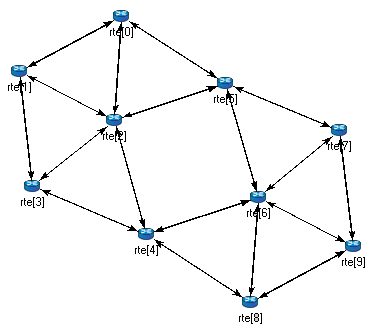
\includegraphics[scale=0.6]{figures/ned-routing-network}
  \caption{The network}
  \label{fig:ned-routing-topology}
\end{figure}

The corresponding NED description would look like this:

\begin{Verbatim}[commandchars=\\\{\}]
//
// A network
//
\tbf{network} Network
\{
    \tbf{submodules}:
        node1: Node;
        node2: Node;
        node3: Node;
        ...
    \tbf{connections}:
        node1.port++ <--> \{datarate=100Mbps;\} <--> node2.port++;
        node2.port++ <--> \{datarate=100Mbps;\} <--> node4.port++;
        node4.port++ <--> \{datarate=100Mbps;\} <--> node6.port++;
        ...
\}
\end{Verbatim}

The above code defines a network type named \ttt{Network}. Note that the NED
language uses the familiar curly brace syntax, and ``\ttt{//}'' to denote
comments.

\begin{note}
    Comments in NED not only make the source code more readable, but in the
    {\opp} IDE they also get displayed at various places (tooltips, content
    assist, etc), and become part of the documentation extracted from the NED
    files. The NED documentation system, not unlike \textit{JavaDoc} or
    \textit{Doxygen}, will be described in Chapter \ref{cha:neddoc}.
\end{note}

The network contains several nodes, named \ttt{node1}, \ttt{node2}, etc.
from the NED module type \ttt{Node}. We'll define \ttt{Node} in the next
sections.

The second half of the declaration defines how the nodes are to be
connected. The double arrow means bidirectional connection. The connection
points of modules are called gates, and the \ttt{port++} notation adds a
new gate to the \ttt{port[]} gate vector. Gates and connections will be
covered in more detail in sections \ref{sec:ch-ned-lang:gates} and
\ref{sec:ch-ned-lang:connections}. Nodes are connected with a channel that
has a data rate of 100Mbps.

\begin{note}
    In many other systems, the equivalent of {\opp} gates are called
    \textit{ports}. We have retained the term \textit{gate} to reduce
    collisions with other uses of the otherwise overloaded word
    \textit{port}: router port, TCP port, I/O port, etc.
\end{note}

The above code would be placed into a file named \ttt{Net6.ned}. It is
a convention to put every NED definition into its own file and to name the
file accordingly, but it is not mandatory to do so.

One can define any number of networks in the NED files, and for every
simulation the user has to specify which network he wants to set up.
The usual way of specifying the network is to put the \fconfig{network}
option into the configuration (by default the \ttt{omnetpp.ini} file):

\begin{Verbatim}
[General]
network = Network
\end{Verbatim}


\subsection{Introducing a channel}

It is cumbersome to have to repeat the data rate for every connection.
Luckily, NED provides a convenient solution: one can create a new channel
type that encapsulates the data rate setting, and this channel type can
be defined inside the network so that it does not litter the global
namespace.

The improved network will look like this:

\begin{Verbatim}[commandchars=\\\{\}]
//
// A Network
//
\tbf{network} Network
\{
    \tbf{types}:
        \tbf{channel} C \tbf{extends} ned.DatarateChannel \{
            datarate = 100Mbps;
        \}
    \tbf{submodules}:
        node1: Node;
        node2: Node;
        node3: Node;
        ...
    \tbf{connections}:
        node1.port++ <--> C <--> node2.port++;
        node2.port++ <--> C <--> node4.port++;
        node4.port++ <--> C <--> node6.port++;
        ...
\}
\end{Verbatim}

Later sections will cover the concepts used (inner types, channels, the
\ttt{DatarateChannel} built-in type, inheritance) in details.


\subsection{The App, Routing and Queue simple modules}

Simple modules are the basic building blocks for other (compound) modules.
All active behavior in the model is encapsulated in simple modules.
Behavior is defined with a C++ class; NED files only declare the externally
visible interface of the module (gates, parameters).

In our example, we could define \ttt{Node} as a simple module. However,
its functionality is quite complex (traffic generation, routing, etc),
so it is better to implement it with several smaller simple module types
which we are going to assemble into a compound module. We'll have
one simple module for traffic generation (\ttt{App}), one for routing
(\ttt{Routing}), and one for queueing up packets to be sent out (\ttt{Queue}).
For brevity, we omit the bodies of the latter two in the code below.

\begin{Verbatim}[commandchars=\\\{\}]
simple App
\{
    \tbf{parameters}:
        \tbf{int} destAddress;
        ...
        @display("i=block/browser");
    \tbf{gates}:
        \tbf{input} in;
        \tbf{output} out;
\}

\tbf{simple} Routing
\{
    ...
\}

\tbf{simple} Queue
\{
    ...
\}
\end{Verbatim}

By convention, the above simple module declarations go into the
\ttt{App.ned}, \ttt{Routing.ned} and \ttt{Queue.ned} files.

\begin{note}
    Note that module type names (\ttt{App}, \ttt{Routing}, \ttt{Queue})
    begin with a capital letter, and parameter and gate names begin with
    lowercase -- this is the recommended naming convention. Capitalization
    matters because the language is case sensitive.
\end{note}

Let us see the first simple module type declaration. \ttt{App} has a
parameter called \ttt{destAddress} (others have been omitted for now),
and two gates named \ttt{out} and \ttt{in} for sending and receiving
application packets.

The argument of \ttt{@display()} is called a \textit{display string},
and it defines the default rendering of the module in graphical environments;
\ttt{"i=..."} defines the default icon.

Generally, \ttt{@}-words like \ttt{@display} are called \textit{properties}
in NED, and they are used to annotate various objects
with metadata. Properties can be attached to files, modules, parameters, gates,
connections, and other objects, and parameter values have a very flexible
syntax.


\subsection{The Node compound module}

Now we can assemble \ttt{App}, \ttt{Routing} and {Queue} into the
compound module \ttt{Node}. A compound module can be thought of as
a ``cardboard box'' that groups other modules into a larger unit,
which can further be used as a building block for other modules;
networks are also a kind of compound module.

\begin{figure}[htbp]
  \centering
  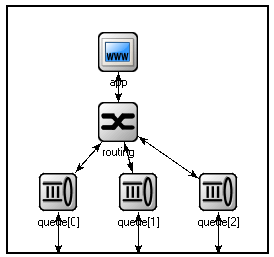
\includegraphics[scale=0.6]{figures/ned-routing-node}
  \caption{The Node compound module}
  \label{fig:ned-routing-node}
\end{figure}

\begin{Verbatim}[commandchars=\\\{\}]
\tbf{module} Node
\{
    \tbf{parameters}:
        @display("i=misc/node_vs,gold");
    \tbf{gates}:
        \tbf{inout} port[];
    \tbf{submodules}:
        app: App;
        routing: Routing;
        queue[\tbf{sizeof}(port)]: Queue;
    \tbf{connections}:
        routing.localOut --> app.in;
        routing.localIn <-- app.out;
        \tbf{for} i=0..\tbf{sizeof}(port)-1 \{
            routing.out[i] --> queue[i].in;
            routing.in[i] <-- queue[i].out;
            queue[i].line <--> port[i];
        \}
\}
\end{Verbatim}

Compound modules, like simple modules, may have parameters and gates.
Our \ttt{Node} module contains an \ttt{address} parameter, plus a
\textit{gate vector} of unspecified size, named \ttt{port}.
The actual gate vector size will be determined implicitly by the number
of neighbours when we create a network from nodes of this type.
The type of \ttt{port[]} is \ttt{inout}, which allows bidirectional
connections.

The modules that make up the compound module are listed under
\fkeyword{submodules}. Our \ttt{Node} compound module type has an \ttt{app} and
a \ttt{routing} \textit{submodule}, plus a \ttt{queue[]} \textit{submodule
vector} that contains one \ttt{Queue} module for each port, as specified by
\ttt{[sizeof(port)]}. (It is legal to refer to \ttt{[sizeof(port)]} because
the network is built in top-down order, and the node is already created and
connected at network level when its submodule structure is built out.)

In the \fkeyword{connections} section, the submodules are connected to each
other and to the parent module. Single arrows are used to connect input and
output gates, and double arrows connect inout gates, and a \fkeyword{for} loop
is utilized to connect the \ttt{routing} module to each \ttt{queue} module, and
to connect the outgoing/incoming link (\ttt{line} gate) of each queue to the
corresponding port of the enclosing module.


\subsection{Putting it together}

We have seen all NED definitions, but how does it get used by {\opp}? When
the simulation program is started, it loads the NED files. The program
should already contain the C++ classes that implement the needed simple
modules, \ttt{App}, \ttt{Routing} and \ttt{Queue}; their C++ code is either
part if the executable or gets loaded from shared library. The simulation
program also loads the configuration (\ttt{omnetpp.ini}), and determines
from it that the simulation model to be run is the \ttt{Network} network.
Then the network gets instantiated for simulation.

The simulation model is built in a top-down preorder fashion. This means
that starting from an empty system module, all submodules are created,
their parameters and vector sizes get assigned and they get fully connected
before proceeding to go into the submodules to build their internals.

%%XXX rename \fname to \ffunc{}!!!

\bigskip
\begin{center}* * *\end{center}
\bigskip

In the following sections we'll go through the elements of the NED
language and look at them in more details.



\section{Simple modules}
\label{sec:ch-ned-lang:simple-modules}

Simple modules are the active components in the model.
Simple modules are defined with the \fkeyword{simple} keyword.

An example simple module:

\begin{Verbatim}[commandchars=\\\{\}]
\tbf{simple} Queue
\{
    \tbf{parameters}:
        \tbf{int} capacity;
        @display("i=block/queue");
    \tbf{gates}:
        \tbf{input} in;
        \tbf{output} out;
\}
\end{Verbatim}

Both the \fkeyword{parameters} and \fkeyword{gates} sections are optional, that is,
they can be left out if there's no parameter or gate. In addition, the
\fkeyword{parameters} keyword itself is optional too, it can be left out
even if there are parameters or properties.

Note that the NED definition doesn't contain any code to define the
operation of the module: that part is expressed in C++. By default, {\opp}
looks for C++ classes of the same name as the NED type (so here, \ttt{Queue}).

One can explicitly specify the C++ class with the \ttt{@class} property.
Classes with namespace qualifiers are also accepted, as shown in the following
example that uses the \ttt{mylib::Queue} class:

\begin{Verbatim}[commandchars=\\\{\}]
\tbf{simple} Queue
\{
    \tbf{parameters}:
        \tbf{int} capacity;
        @class(mylib::Queue);
        @display("i=block/queue");
    \tbf{gates}:
        \tbf{input} in;
        \tbf{output} out;
\}
\end{Verbatim}

If you have several modules that are all in a common namespace, then a
better alternative to \ttt{@class} is the \ttt{@namespace} property. The
C++ namespace given with \ttt{@namespace} will be prepended to the normal
class name. In the following example, the C++ classes will be
\ttt{mylib::App}, \ttt{mylib::Router} and \ttt{mylib::Queue}:

\begin{Verbatim}[commandchars=\\\{\}]
@namespace(mylib);

\tbf{simple} App \{
   ...
\}

\tbf{simple} Router \{
   ...
\}

\tbf{simple} Queue \{
   ...
\}
\end{Verbatim}

As you've seen, \ttt{@namespace} can be specified on file level. Moreover,
when placed in a file called \ttt{package.ned}, the namespace will apply to
all files in the same directory and all directories below.

The implementation C++ classes need to be subclassed from the
\cclass{cSimpleModule} library class; chapter \ref{cha:simple-modules} of
this manual describes in detail how to write them.

Simple modules can be extended (or specialized) via subclassing. The
motivation for subclassing can be to set some open parameters or gate sizes
to a fixed value (see \ref{sec:ch-ned-lang:parameters} and
\ref{sec:ch-ned-lang:gates}), or to replace the C++ class with a different
one. Now, by default the derived NED module type will \textit{inherit} the
C++ class from its base, so it is important to remember that you need to
write out \ttt{@class} if you want it to use the new class.

The following example shows how to specialize a module by setting a parameter
to a fixed value (and leaving the C++ class unchanged):

\begin{Verbatim}[commandchars=\\\{\}]
\tbf{simple} Queue
\{
   \tbf{int} capacity;
   ...
\}

\tbf{simple} BoundedQueue \tbf{extends} Queue
\{
   capacity = 10;
\}
\end{Verbatim}

In the next example, the author wrote a \ttt{PriorityQueue} C++ class, and
wants to have a corresponding NED type, derived from \ttt{Queue}. However,
it does not work as expected:

\begin{Verbatim}[commandchars=\\\{\}]
\tbf{simple} PriorityQueue \tbf{extends} Queue // wrong! still uses the Queue C++ class
\{
\}
\end{Verbatim}

The correct solution is to add a \ttt{@class} property to override the
inherited C++ class:

\begin{Verbatim}[commandchars=\\\{\}]
\tbf{simple} PriorityQueue \tbf{extends} Queue
\{
   @class(PriorityQueue);
\}
\end{Verbatim}

Inheritance in general will be discussed in section \ref{sec:ch-ned-lang:inheritance}.



\section{Compound modules}
\label{sec:ch-ned-lang:compound-modules}

A compound module groups other modules into a larger unit. A compound
module may have gates and parameters like a simple module, but
no active behavior (no C++ code) is associated with it.

\begin{note}
    When there is a temptation to add code to a compound module,
    then encapsulate the code into a simple module, and add it as
    a submodule.
\end{note}

A compound module declaration may contain several sections,
all of them optional:

\begin{Verbatim}[commandchars=\\\{\}]
\tbf{module} Host
\{
   \tbf{types}:
       ...
   \tbf{parameters}:
       ...
   \tbf{gates}:
       ...
   \tbf{submodules}:
       ...
   \tbf{connections}:
       ...
\}
\end{Verbatim}

Modules contained in a compound module are called submodules, and they are
listed in the \ttt{submodules} section. One can create arrays of submodules
(i.e. submodule vectors), and the submodule type may come from a parameter.

Connections are listed under the \ttt{connections} section of the
declaration. One can create connections using simple programming constructs
(loop, conditional). Connection behaviour can be defined by associating a
channel with the connection; the channel type may also come from a
parameter.

Module and channel types only used locally can be defined in the
\ttt{types} section as inner types, so that they don't pollute the
namespace.

Compound modules may be extended via subclassing. Inheritance may add new
submodules and new connections as well, not only parameters and gates;
also, one may refer to inherited submodules, to inherited types etc. What
is not possible is to "de-inherit" submodules or connections, or to modify
inherited ones.

In the following example, we show how one can assemble common protocols
into a "stub" for wireless hosts, and add user agents via
subclassing.\footnote{Module types, gate names, etc. used in the example
are fictional, not based on an actual {\opp}-based model framework}

\begin{Verbatim}[commandchars=\\\{\}]
\tbf{module} WirelessHostBase
\{
   \tbf{gates}:
       \tbf{input} radioIn;
   \tbf{submodules}:
       tcp: TCP;
       ip: IP;
       wlan: Ieee80211;
   \tbf{connections}:
       tcp.ipOut --> ip.tcpIn;
       tcp.ipIn <-- ip.tcpOut;
       ip.nicOut++ --> wlan.ipIn;
       ip.nicIn++ <-- wlan.ipOut;
       wlan.radioIn <-- radioIn;
\}

\tbf{module} WirelessUser \tbf{extends} WirelessHostBase
\{
   \tbf{submodules}:
       webAgent: WebAgent;
   \tbf{connections}:
       webAgent.tcpOut --> tcp.appIn++;
       webAgent.tcpIn <-- tcp.appOut++;
\}
\end{Verbatim}

The \ttt{WirelessUser} compound module can further be extended,
for example with an Ethernet port:

\begin{Verbatim}[commandchars=\\\{\}]
\tbf{module} DesktopUser \tbf{extends} WirelessUser
\{
   \tbf{gates}:
       \tbf{inout} ethg;
   \tbf{submodules}:
       eth: EthernetNic;
   \tbf{connections}:
       ip.nicOut++ --> eth.ipIn;
       ip.nicIn++ <-- eth.ipOut;
       eth.phy <--> ethg;
\}
\end{Verbatim}



\section{Channels}
\label{sec:ch-ned-lang:channels}

Channels encapsulate parameters and behaviour associated with connections.
Channels are like simple modules, in the sense that there are C++ classes
behind them. The rules for finding the C++ class for a NED channel type is
the same as with simple modules: the default class name is the NED type
name unless there is a \ttt{@class} property (\ttt{@namespace} is also
observed), and the C++ class is inherited when the channel is subclassed.

Thus, the following channel type would expect a \ttt{CustomChannel} C++ class
to be present:

\begin{Verbatim}[commandchars=\\\{\}]
\tbf{channel} CustomChannel  // needs a CustomChannel C++ class
\{
\}
\end{Verbatim}

The practical difference to modules is that you rarely need to write you own
channel C++ class, because there are predefined channel types that you can
subclass from, inheriting their C++ code. The predefined types are:
\ttt{ned.IdealChannel}, \ttt{ned.Delay\-Channel} and \ttt{ned.Datarate\-Channel}.
(``\ttt{ned}'' is the package name; you can get rid of it if you import the types
with the \ttt{import ned.*} or similar directive. Packages and imports
are described in section \ref{sec:ch-ned-lang:packages}.)

\ttt{IdealChannel} has no parameters, and lets through all messages without
delay or any side effect. A connection without a channel object
and a connection with an \ttt{IdealChannel} behave in the same way.
Still, \ttt{IdealChannel} has its uses, for example when a channel object
is required so that it can carry a new property or parameter that is
going to be read by other parts of the simulation model.

\ttt{DelayChannel} has two parameters:

\begin{itemize}
    \item \ttt{delay} is a \ttt{double} parameter which represents the
          propagation delay of the message. Values need to be specified
          together with a time unit (\ttt{s}, \ttt{ms}, \ttt{us}, etc.)
    \item \ttt{disabled} is a boolean parameter that defaults to \ttt{false};
          when set to \ttt{true}, the channel object will drop all messages.
\end{itemize}

\ttt{DatarateChannel} has a few additional parameters compared to \ttt{DelayChannel}:

\begin{itemize}
    \item \ttt{datarate} is a \ttt{double} parameter that represents the
          bandwidth of the channel, and it is used for calculating the
          transmission duration of packets. Values need to be specified
          with bits per second or its multiples as unit (\ttt{bps},
          \ttt{Kbps}, \ttt{Mbps}, \ttt{Gbps}, etc.) Zero is treated
          specially and results in zero transmission duration, i.e.
          it stands for infinite bandwidth. Zero is also the default.
    \item \ttt{ber} and \ttt{per} stand for Bit Error Rate and Packet Error Rate,
          and allow basic error modelling. They expect a \ttt{double}
          in the $[0,1]$ range. When the channel decides (based on random
          numbers) that an error occurred during transmission a packet,
          it sets an error flag in the packet object. The receiver
          module is expected to check the flag, and discard the packet
          as corrupted if it is set. The default \ttt{ber} and \ttt{per}
          are zero.
\end{itemize}

\begin{note}
    XXX "deliver on first bit": this can be specified in C++
\end{note}

The following example shows how to create a new channel type by
specializing \ttt{DatarateChannel}:

\begin{Verbatim}[commandchars=\\\{\}]
\tbf{channel} C \tbf{extends} ned.DatarateChannel
\{
    datarate = 100Mbps;
    delay = 100us;
    ber = 1e-10;
\}
\end{Verbatim}

\begin{note}
    The three built-in channel types are also used for connections where
    the channel type not explicitly specified.
\end{note}

You may add parameters and properties to channels via subclassing, and
modify existing ones. In the following example, we introduce length-based
calculation of the propagation delay:

\begin{Verbatim}[commandchars=\\\{\}]
\tbf{channel} DatarateChannel2 \tbf{extends} ned.DatarateChannel
\{
    \tbf{double} length @unit(m);
    \tbf{delay} = \tbf{this}.length / 200000km * 1s;
\}
\end{Verbatim}

Parameters are primarily useful as input to the underlying C++ class, but
even if you reuse the underlying C++ class of built-in channel types, they
may be read and used by other parts of the model. For example, adding a
\ttt{cost} parameter (or \ttt{@cost} property) may be observed by the
routing algorithm and used for routing decisions. The following example
shows a \ttt{cost} parameter, and annotation using a property
(\ttt{@backbone}).

\begin{Verbatim}[commandchars=\\\{\}]
\tbf{channel} Backbone \tbf{extends} ned.DatarateChannel
\{
    @backbone;
    \tbf{double} cost = \tbf{default}(1);
\}
\end{Verbatim}



\section{Parameters}
\label{sec:ch-ned-lang:parameters}

Parameters are variables that belong to a module. Parameters can be
used in building the topology (number of nodes, etc), and to supply
input to C++ code that implements simple modules and channels.

Parameters can be of type \fkeyword{double}, \fkeyword{int},
\fkeyword{bool}, \fkeyword{string} and \fkeyword{xml}; they can also
be declared \fkeyword{volatile}. For the numeric types, a unit of
measurement can also be specified (\ttt{@unit} property), to increase
type safety.

Parameters can get their value from NED files or from the configuration
(\ttt{omnetpp.ini}). A default value can also be given (\ttt{default(}...\ttt{)}),
which gets used if the parameter is not assigned otherwise.

Let use see an example before we go into details:

\begin{Verbatim}[commandchars=\\\{\}]
\tbf{simple} App
\{
    \tbf{parameters}:
        \tbf{int} address;  // local node address
        \tbf{string} destAddresses;  // destination addresses
        \tbf{volatile double} sendIaTime @unit(s) = \tbf{default}(exponential(1s));
                               // time between generating packets
        \tbf{volatile int} packetLength @unit(byte);  // length of one packet
    ...
\}
\end{Verbatim}

\subsubsection{Values}

may be assigned in submodules

via inheritance  (examples!!!)

in the configuration

C-like expression etc

\subsubsection{volatile}

The \fkeyword{volatile} modifier causes the parameter's value expression to
be evaluated every time the parameter is read. This has significance if the
expression is not constant, for example it involves numbers drawn from a
random number generator. In contrast, non-volatile parameters are evaluated
only once. (This practically means that they are evaluated and replaced
with the resulting constant at the start of the simulation.)

To better understand \fkeyword{volatile}, let's suppose we have an
\ttt{ActiveQueue} simple module that has a \ttt{volatile double} parameter
named \ttt{serviceTime}.

XXX ??? random serviceTime altalaban hulyeseg, maradjunk az iatime-nel

The queue module's C++ implementation would re-read the \ttt{serviceTime}
parameter at runtime for every job serviced; so if \ttt{serviceTime} is
assigned an expression like \ttt{uniform(0.5s, 1.5s)}, every job would have
a different, random service time.

In practice, a volatile parameter usually means that the underlying C++
code will re-read the parameter every time a value is needed at runtime, so
the parameter can be used a source of random numbers.

\begin{note}
    This does not mean that a non-volatile parameter cannot be assigned a value
    like \ttt{uniform(0.5s, 1.5s)}. It can, but that has a totally different
    effect. Had we omitted the \ttt{volatile} keyword from the
    \ttt{serviceTime} parameter, for example, the effect would be that every
    job had the \textit{same} constant service time, say \ttt{1.2975367s},
    chosen randomly at the beginning of the simulation.
\end{note}

\subsubsection{Units}

One can declare a parameter to have an associated unit of measurement,
by adding the \ttt{@unit} property.

The \ttt{serviceTime} parameter is decorated with \ttt{@unit(s)}. This means
that the value must be specified in either seconds, or in a measurement unit {\opp}
can convert to seconds, like milliseconds or hours; dimensionless numbers
will not be accepted. The {\opp} runtime does a full and rigorous unit check on
parameters to ensure ``unit safety'' of models.

XXX example

XXX @unit cannot be overridden in subclasses or in a submodule declaration

XXX see \_\_SCRATCH for more....


\subsubsection{XML parameters}

Sometimes modules need more complex input than simple module parameters
can describe. Then you'd put these parameters into an external config file,
and let the modules read and process the file. You'd pass the file name
to the modules in a string parameter.

These days, XML is increasingly becoming a standard format for configuration
files as well, so you might as well describe your configuration in XML.
From the 3.0 version, {\opp} contains built-in support for XML config files.

{\opp} wraps the XML parser (LibXML, Expat, etc.), reads and DTD-validates
the file (if the XML document contains a DOCTYPE), caches the file
(so that if you refer to it from several modules, it'll still be loaded
only once), lets you pick parts of the document via an XPath-subset notation,
and presents the contents to you in a DOM-like object tree.

This machinery can be accessed via the NED parameter type \ttt{xml}, and the
\ttt{xmldoc()} operator. You can point \ttt{xml}-type module parameters
to a specific XML file (or to an element inside an XML file) via the
\ttt{xmldoc()} operator. You can assign \ttt{xml} parameters both from NED
and from \ttt{omnetpp.ini}.

XXX add a complete example!

\begin{Verbatim}[commandchars=\\\{\}]
\tbf{simple} TrafficGenerator \{
    \tbf{parameters}:
        \tbf{xml} profile;
    \tbf{gates}:
        \tbf{output} out;
\}

\tbf{module} TrafficGenerator \{
    XXX several submods, and assign!
    \tbf{parameters}:
        \tbf{xml} profile;
    \tbf{gates}:
        \tbf{output} out;
\}
\end{Verbatim}

XXX example 2, with xpath!

\section{Gates}
\label{sec:ch-ned-lang:gates}

Gates are the connection points of modules.  {\opp} has three types of
gates: \textit{input}, \textit{output} and \textit{inout}, the latter being
essentially an input and an output gate glued together.

A gate, whether input or output, cannot be connected to two or more other
gates. (For compound module gates, this means one connection "outside" and
one "inside".)  It is possible, though generally not recommended, to
connect the input and output sides of an inout gate separately.

One can create single gates and gate vectors. The size of a gate vector
can be given inside square brackets in the declaration, but it also possible
to leave it open by just writing a pair of empty brackets ("\ttt{[]}").

When the gate vector size is left open, one can still specify it later,
when subclassing the module, or when using the module for a submodule in a
compound module. However, it does not need to be specified, because
one can create connections with the \ttt{$gate$++} operator that
automatically expands the gate vector.

The gate size can be queried from various NED expressions with the
\ttt{sizeof()} operator.

NED normally requires that all gates be connected. To relax this
requirement, you can annotate selected gates with the \ttt{@loose}
property, which turns off connectivity check for that gate. Also, input
gates that solely exist so that the module can receive messages via
\fname{sendDirect()} (see \ref{sec:simple-modules:direct-sending}) should
be annotated with \ttt{@directIn}. (\ttt{@directIn} gates must remain
unconnected.) It is also possible to turn off connectivity check for all
gates within a compound module, by specifying the
\fkeyword{allowunconnected} keyword in the module's connections section.

Let us see some examples.

In the following example, the \ttt{Classifier} module has one input for
receiving jobs, which it will send to one of the outputs. The number of
outputs is determined by a module parameter:

\begin{Verbatim}[commandchars=\\\{\}]
\tbf{simple} Classifier \{
    \tbf{parameters}:
        \tbf{int} numCategories;
    \tbf{gates}:
        \tbf{input} in;
        \tbf{output} out[numCategories];
\}
\end{Verbatim}

The following \ttt{Sink} module also has its \ttt{in[]} gate defined
as vector, so that it can be connected to several modules:

\begin{Verbatim}[commandchars=\\\{\}]
\tbf{simple} Sink \{
    \tbf{gates}:
        \tbf{input} in[];
\}
\end{Verbatim}

A node for building a square grid. Gates around the edges of the grid are
expected to remain unconnected, hence the \ttt{@loose} annotation:

\begin{Verbatim}[commandchars=\\\{\}]
\tbf{simple} GridNode \{
    \tbf{gates}:
        \tbf{inout} neighbour[4] @loose;
\}
\end{Verbatim}

\ttt{WirelessNode} below is expected to receive messages (radio transmissions)
via direct sending, so its \ttt{radioIn} gate is marked with \ttt{@directIn}.

\begin{Verbatim}[commandchars=\\\{\}]
\tbf{simple} WirelessNode \{
    \tbf{gates}:
        \tbf{input} radioIn @directIn;
\}
\end{Verbatim}

In the following example, we define \ttt{TreeNode} as having gates to connect
any number of children, then subclass it to get a \ttt{BinaryTreeNode} to
set the gate size to two:

\begin{Verbatim}[commandchars=\\\{\}]
\tbf{simple} TreeNode \{
    \tbf{gates}:
        \tbf{inout} parent;
        \tbf{inout} children[];
\}

\tbf{simple} BinaryTreeNode \tbf{extends} TreeNode \{
    \tbf{gates}:
        children[2];
\}
\end{Verbatim}

An example for setting the gate vector size in a submodule, using the same
\ttt{TreeNode} module type as above:

\begin{Verbatim}[commandchars=\\\{\}]
\tbf{module} BinaryTree \{
    \tbf{submodules}:
        nodes[31]: TreeNode \{
            \tbf{gates}:
                children[2];
        \}
    \tbf{connections}:
        ...
\}
\end{Verbatim}



\section{Submodules}
\label{sec:ch-ned-lang:submodules}

Modules a compound module consist of are called its submodules.
A submodule has a name, and it is an instance of a compound or simple
module type. In the NED definition of a submodule, this module type
may be explicitly written, but, as we'll see later, it is also possible
to specify the type with a string expression (see section
\ref{sec:ch-ned-lang:submodule-like}.)

NED supports submodule arrays (vectors) as well. Submodule vector size,
unlike gate vector size, must always be specified and cannot be left
open as with gates.

Syntactically, a submodule may have a curly brace block as body, where
it is possible to assign parameters (see \ttt{address} in the example),
set the size of gate vectors, and add/modify properties like the
display string (\ttt{@display}).

XXX kettevenni a kovetkezo peldat:
\begin{Verbatim}[commandchars=\\\{\}]
\tbf{module} Node
\{
    \tbf{gates}:
        \tbf{inout} port[];
    \tbf{submodules}:
        routing: Routing \{
            \tbf{parameters}:   // this keyword is optional
                routingTable = "routingtable.txt"; // assign parameter
            \tbf{gates}:
                in[\tbf{sizeof}(port)];  // set gate vector size
                out[\tbf{sizeof}(port)];
        \}

        queue[\tbf{sizeof}(port)]: Queue;

    \tbf{connections}:
        ...
\}
\end{Verbatim}

A submodule vector may also be used to implement a conditional submodule:

\begin{Verbatim}[commandchars=\\\{\}]
\tbf{module} Host
\{
    \tbf{parameters}:
        \tbf{bool} withTCP = \tbf{default}(\tbf{true});
    \tbf{submodules}:
        tcp[withTCP ? 1 : 0]: TCP;
        ...
    \tbf{connections}:
        tcp[0].ipOut --> ip.tcpIn \tbf{if} withTCP;
        tcp[0].ipIn <-- ip.tcpOut \tbf{if} withTCP;
        ...
\}
\end{Verbatim}

An empty body may be omitted, that is,

\begin{Verbatim}[commandchars=\\\{\}]
      queue: Queue;
\end{Verbatim}

is the same as

\begin{Verbatim}[commandchars=\\\{\}]
      queue: Queue \{
      \}
\end{Verbatim}

Display strings specified here will be merged with the display string
from the type to get the effective display string. This is described
in chapter \ref{cha:graphics}.

It is possible to add new submodules to an existing compound module via
subclassing.

XXX example.



\section{Connections}
\label{sec:ch-ned-lang:connections}

Connections are defined in the \fkeyword{connections} section of compound
modules. Connections cannot span across hierarchy levels: one can connect
two submodule gates, a submodule gate and the "inside" of the parent
(compound) module's gates, or two gates of the parent module (though this
is rarely useful). It is not possible to connect to any gate outside the
parent module, or inside compound submodules.

Input and output gates are connected with a normal arrow, and inout gates
with a double-headed arrow ``\ttt{<-{}->}''. To connect the two gates
with a channel, use two arrows and put the channel specification in between.

Some examples have already been shown in the Warmup section
(\ref{sec:ch-ned-lang:warmup}); let's see some more.

XXX examples

XXX explain \$i / \$o

XXX explain ++


\subsubsection{Channel specification}

A channel specification (\ttt{-{}-> $channelspec$ -{}->} inside a connection)
are similar to submodules in many respect.

Let's see some examples:

\begin{Verbatim}[commandchars=\\\{\}]
<--> {delay=10ms;} <-->
<--> {delay=10ms; datarate=1e-8;} <-->
<--> C <-->
<--> BBone {cost=100; length=52km; datarate=1e-8;} <-->
<--> {@display("XXX");} <-->
<--> BBone {@display("XXX");} <-->
\end{Verbatim}


When a channel type is missing, one of the built-in channel types will be
used, based on the parameters assigned in the connection. If
\ttt{datarate}, \ttt{ber} or \ttt{per} is assigned,
\ttt{ned.DatarateChannel} will be chosen. Otherwise, if \ttt{delay} or
\ttt{disabled} is present, it will be \ttt{ned.DelayChannel}; otherwise it
is \ttt{ned.IdealChannel}. Naturally, if other parameter names are
assigned in an connection without an explicit channel type, it will be an error
(with \textit{``ned.DelayChannel has no such parameter''} or similar message).

XXX channel type as parameter; here or later?


\section{Multiple connections}
\label{sec:ch-ned-lang:multiple-connections}

Simple programming constructs (loop, conditional) allow creating
multiple connections easily.

Example...

Let use see more connection examples.

\subsubsection{Chain}

One can create a chain\index{chain} of modules like this:

\begin{Verbatim}[commandchars=\\\{\}]
\tbf{module} Chain
    \tbf{parameters}:
        \tbf{int} count;
    \tbf{submodules}:
        node[count] : Node \{
            \tbf{gates}:
                port[2];
        \}
    \tbf{connections allowunconnected}:
        \tbf{for} i = 0..count-2 \{
            node[i].port[1] <--> node[i+1].port[0];
        \}
\}
\end{Verbatim}


\subsubsection{Binary Tree}

One can build a binary tree\index{binary tree} in the following way:

\begin{Verbatim}[commandchars=\\\{\}]
\tbf{simple} BinaryTreeNode \{
    \tbf{gates}:
        \tbf{inout} left;
        \tbf{inout} right;
        \tbf{inout} parent;
\}

\tbf{module} BinaryTree \{
    \tbf{parameters}:
        \tbf{int} height;
    \tbf{submodules}:
        node[2^height-1]: BinaryTreeNode;
    \tbf{connections} \tbf{allowunconnected}:
        \tbf{for} i=0..2^(height-1)-2 \{
            node[i].left <--> node[2*i+1].parent;
            node[i].right <--> node[2*i+2].parent;
        \}
\}
\end{Verbatim}

Note that not every gate of the modules will be connected. By default,
an unconnected gate produces a run-time error message when the
simulation is started, but this error message is turned off here with
the \fkeyword{allowunconnected} modifier.
Consequently, it is the simple modules' responsibility not to send
on a gate which is not leading anywhere.



\subsubsection{Random graph}

Conditional connections can be used to generate random
topologies\index{topology!random}, for example. The following code
generates a random subgraph of a full graph:

\begin{Verbatim}[commandchars=\\\{\}]
\tbf{module} RandomGraph \{
    \tbf{parameters}:
        \tbf{int} count;
        \tbf{double} connectedness; // 0.0<x<1.0
    \tbf{submodules}:
        node[count]: Node \{
            \tbf{gates}:
                in[count];
                out[count];
        \}
    \tbf{connections} \tbf{allowunconnected}:
        \tbf{for} i=0..count-1, j=0..count-1 \{
            node[i].out[j] --> node[j].in[i]
                \tbf{if} i!=j && uniform(0,1)<connectedness;
        \}
\}
\end{Verbatim}

Note the use of the \fkeyword{allowunconnected} modifier
here too, to turn off error messages given by the network setup code
for unconnected gates.


\subsection{Connection patterns}

\index{module!compound!patterns}
\index{topology!patterns}

Several approaches can be used when you want to create complex
topologies which have a regular structure; three of them are
described below.


\subsubsection{``Subgraph of a Full Graph''}


This pattern takes a subset of the connections of a full graph.  A
condition is used to ``carve out'' the necessary interconnection from
the full graph:

\begin{Verbatim}[commandchars=\\\{\}]
\tbf{for} i=0..N-1, j=0..N-1 \{
    node[i].out[...] --> node[j].in[...] \tbf{if} condition(i,j);
\}
\end{Verbatim}

The RandomGraph compound module (presented earlier) is an example of
this pattern, but the pattern can generate any graph where an
appropriate $condition(i,j)$ can be formulated. For example,
when generating a tree\index{topology!tree} structure, the condition
would return whether node $j$ is a child of node $i$ or
vica versa.

Though this pattern is very general, its usage can be prohibitive if
the $N$ number of nodes is high and the graph is sparse (it has
much fewer connections that $N^2$). The following
two patterns do not suffer from this drawback.


\subsubsection{``Connections of Each Node''}

The pattern loops through all nodes and creates the necessary
connections for each one. It can be generalized like this:

\begin{Verbatim}[commandchars=\\\{\}]
\tbf{for} i=0..Nnodes, j=0..Nconns(i)-1 \{
    node[i].out[j] --> node[rightNodeIndex(i,j)].in[j];
\}
\end{Verbatim}

The Hypercube\index{topology!hypercube} compound module (to be
presented later) is a clear example of this approach. BinaryTree can
also be regarded as an example of this pattern where the inner j loop
is unrolled.

The applicability of this pattern depends on how easily the $rightNodeIndex(i,j)$
function can be formulated.


\subsubsection{``Enumerate All Connections''}


A third pattern is to list all connections within a loop:

\begin{Verbatim}[commandchars=\\\{\}]
\tbf{for} i=0..Nconnections-1 \{
    node[leftNodeIndex(i)].out[...] --> node[rightNodeIndex(i)].in[...];
\}
\end{Verbatim}

The pattern can be used if $leftNodeIndex(i)$ and $rightNodeIndex(i)$
mapping functions can be sufficiently formulated.

The \ttt{Chain} module is an example of this approach where the mapping
functions are extremely simple: $leftNodeIndex(i)=i$ and $rightNodeIndex(i) = i+1$.
The pattern can also be used to create a random subset of a full
graph with a fixed number of connections.

In the case of irregular structures where none of the above patterns
can be employed, you can resort to listing all connections, like you
would do it in most existing simulators.



\section{Submodule type as parameter}
\label{sec:ch-ned-lang:submodule-like}

A submodule type may be specified with a module parameter of the type
\fkeyword{string}, or in general, with any string-typed expression.
The syntax uses the \fkeyword{like} keyword.

Let us begin with an example:

\begin{Verbatim}[commandchars=\\\{\}]
\tbf{network} Net6
\{
    \tbf{parameters}:
        \tbf{string} nodeType;
    \tbf{submodules}:
        node[6]: <nodeType> \tbf{like} INode \{
            address = \tbf{index};
        \}
    \tbf{connections}:
        ...
\}
\end{Verbatim}

It creates a submodule vector whose module type will come from the
\ttt{nodeType} parameter. For example, if \ttt{nodeType="SensorNode"},
then the module vector will consist of sensor nodes (provided such module
type exists and it qualifies -- the latter will be explained right now).

The missing piece is the \ttt{like INode} bit. \ttt{INode} must be
an existing \textit{module interface}, which the \ttt{SensorNode}
module type must implement (more about this later).

The corresponding NED declarations:

\begin{Verbatim}[commandchars=\\\{\}]
\tbf{moduleinterface} INode
\{
    \tbf{parameters}:
        \tbf{int} address;
    \tbf{gates}:
        \tbf{inout} port[];
\}
\end{Verbatim}

\begin{Verbatim}[commandchars=\\\{\}]
\tbf{module} SensorNode \tbf{like} INode
\{
    \tbf{parameters}:
        \tbf{int} address;
        ...
    \tbf{gates}:
        \tbf{inout} port[];
        ...
\}
\end{Verbatim}

of course, typ
XXX expressions accepted; show a some examples
XXX Note: parser may get confused around <>; you may help it by adding parens, i.e. <(typeName+"Module")>


\section{Properties (metadata annotations)}
\label{sec:ch-ned-lang:properties}

Properties allow adding metadata annotations to modules, parameters, gates,
connections, NED files, packages, and virtually anything in NED.
\ttt{@display}, \ttt{@class}, \ttt{@namespace}, \ttt{@unit}, \ttt{@prompt},
\ttt{@loose}, \ttt{@directIn} are all properties that have been mentioned in
previous sections, but those examples only scratch the surface of what can
be done with properties.

XXX @isNetwork (valahol leirni azt is; BTW "network" nincs leirva sectionben)

Using properties, one can attach extra information to NED elements. Some
properties are interpreted by NED, by the simulation kernel; other
properties may be read and used from within the simulation model, or
provide hints for NED editing tools.

Properties are attached to the type, so you cannot have properties
per-instance different properties. All instances of modules, connections,
parameters, etc. created from any particular location in the NED files have
identical properties.

The following example shows the syntax for annotating various NED elements:

\begin{Verbatim}[commandchars=\\\{\}]
@prop;  // file property

\tbf{module} Example
\{
    \tbf{parameters}:
       @prop;   // module property
       \tbf{int} a @prop = \tbf{default}(1); // parameter property
    \tbf{gates}:
       \tbf{output} out @prop;
    \tbf{submodules}:
       src: Source \{
           \tbf{parameters}:
              @prop;  // submodule property
              count @prop;  // adding a property to a parameter
           \tbf{gates}:
              out[] @prop;  // adding a property to a gate
       \}
       ...
    \tbf{connections}:
       src.out++ --> \{ @prop; \} --> sink1.in;
       src.out++ --> Channel \{ @prop; \} --> sink2.in;
\}
\end{Verbatim}


\subsubsection{Data model}

Properties may contain data, given in parentheses; the data model is quite
flexible. Properties may contain lists:

\begin{Verbatim}[commandchars=\\\{\}]
@enum(Sneezy,Sleepy,Dopey,Doc,Happy,Bashful,Grumpy);
\end{Verbatim}

They may contain key-value pairs, separated by semicolons:

\begin{Verbatim}[commandchars=\\\{\}]
@coords(x=10.31; y=30.2; unit=km);
\end{Verbatim}

In key-value pairs, each value can be a (comma-separated) list:

\begin{Verbatim}[commandchars=\\\{\}]
@nodeinfo(id=742;labels=swregion,routers,critical);
\end{Verbatim}

The above examples are special cases of the general data model. According
to the data model, properties contain \textit{key-valuelist} pairs,
separated by semicolons. Items in \textit{valuelist} are separated by
commas. Wherever \textit{key} is missing, values go on the valuelist of the
\textit{default key}, the empty string. \ttt{@prop} is the same
as \ttt{@prop()}.

The syntax for value items is a bit restrictive: they may contain words,
numbers, string constants and some more, but not arbitrary strings.
Whenever the syntax does not permit some value, it should be enclosed in
quotes. This quoting does not make any difference in the value, because
the parser automatically drops one layer of quotes; thus, \ttt{@class(TCP)}
and \ttt{@class("TCP")} are exactly the same.

There are also some conventions. One can use properties to tag some NED element
with a label; for example, a \ttt{@host} property could be used to mark
all module types that represent various hosts. This property could be used
e.g. by editing tools, by topology discovery code inside the simulation model, etc.

The convention for such a "label" property is that any extra data in it
(i.e. within parens) is ignored, except a single word \ttt{false}, which is
reserved to "remove" the property. Thus, simulation model or tool source
code that interprets properties should handle all the following forms as
equivalent to \ttt{@host}: \ttt{@host()}, \ttt{@host(true)},
\ttt{@host(anything-but-false)}, \ttt{@host(a=1;b=2)}; and
\ttt{@host(false)} should be interpreted as the lack of the \ttt{@host}
tag.


\subsubsection{Modifying properties}

When you subclass a NED type, use a module type as submodule or use a channel
type for a connection, you may add new properties to the module or channel,
or to its parameters and gates, and you can also modify existing properties.

When modifying a property, the new property gets merged with the old one,
with a few simple rules. New keys simply get added. If a key already
exists in the old property, items in its valuelist overwrite items on
the same position in the old property. A single hyphen ($-$) as
valuelist item serves as ``antivalue'', it removes the item at the
corresponding position.

Some examples:

\begin{tabular}{l l}
$base$   & \ttt{@prop}  \\
$new$    & \ttt{@prop(a)}  \\
\hline
$result$ & \ttt{@prop(a)}
\end{tabular}

\begin{tabular}{l l}
$base$   & \ttt{@prop(a,b,c)}  \\
$new$    & \ttt{@prop(,-)}  \\
\hline
$result$ & \ttt{@prop(a,{},c)}
\end{tabular}

\begin{tabular}{l l}
$base$   & \ttt{@prop(foo=a,b)}  \\
$new$    & \ttt{@prop(foo=A,{},c;bar=1,2)}  \\
\hline
$result$ & \ttt{@prop(foo=A,b,c;bar=1,2)}
\end{tabular}

\begin{note}
    The above merge rules are part of NED, but the code that interprets
    properties may have special rules for certain properties. For example,
    the \ttt{@unit} property of parameters is not allowed to be overridden,
    and \ttt{@display} is merged with special although similar rules
    (see Chapter \ref{cha:graphics}).
\end{note}



\subsubsection{Indices}

Properties are identified by names, so if the same \textit{@$name$} occurs
in the same context, then it names the exact same property object. If you
want to have multiple properties with the same name, then you need to
distinguish them with an index. An index is a name or number, written in
square brackets after the property name. The index may be chosen to carry
a meaning, or it may be a dummy whose only purpose is to tell multiple
properties with the same name apart. (The code that interprets properties
may be written to observe or to ignore indices, as needed).

The following example, the simple module declares in properties the
statistics it collects. These declarations might be used by model editing
tools, by simulation code, or by analysis tools.\footnote{Note that this is
a completely hypothetical example -- {\opp} does not presently support
declaring statistics using properties.} The statistic names are
used as indices:

\begin{Verbatim}[commandchars=\\\{\}]
\tbf{simple} App \{
    // declare two statistics collected by the C++ code
    @statistic[packetsReceived](type=integer;label="Number of packets received");
    @statistic[responseTime](type=double;unit=s;label="Application response time");
    ...
\}

\tbf{simple} HttpApp \tbf{extends} App \{
    // tailor the label of the "packetsReceived" statistic:
    @statistic[packetsReceived](label="Number of HTTP requests received");
\}
\end{Verbatim}



\section{Inheritance}
\label{sec:ch-ned-lang:inheritance}

Inheritance support in the NED language is only described briefly here,
because several details and examples have been already presented in
previous sections.

In NED, a type may only extend (\fkeyword{extends} keyword) an element of
the same component type: a simple module may only extend a simple module,
compound module may only extend a compound module, and so on. Single
inheritance is supported for modules and channels, and multiple inheritance
is supported for module interfaces and channel interfaces. A network is a
shorthand for a compound module with the \ttt{@isNetwork} property set, so
the same rules apply to it as to compound modules.

However, a simple or compound module type may implement (\fkeyword{like}
keyword) several module interfaces; likewise, a channel type may implement
several channel interfaces.

\begin{important}
    When you extend a simple module type both in NED and in C++, you must
    use the \ttt{@class} property to tell NED to use the new C++ class --
    otherwise your new module type inherits the C++ class of the base!
\end{important}

Inheritance may:
\begin{itemize}
    \item add new properties, parameters, gates, inner types, submodules,
          connections, as long as names do not conflict with inherited names
    \item modify inherited properties, and properties of inherited parameters and
          gates
    \item it may not modify inherited submodules, connections and inner types
\end{itemize}

For details and examples, see the corresponding sections of this chapter
(simple modules \ref{sec:ch-ned-lang:simple-modules},
compound modules \ref{sec:ch-ned-lang:compound-modules},
channels \ref{sec:ch-ned-lang:channels},
parameters \ref{sec:ch-ned-lang:parameters},
gates \ref{sec:ch-ned-lang:gates},
submodules \ref{sec:ch-ned-lang:submodules},
connections \ref{sec:ch-ned-lang:connections},
module interfaces and channel interfaces \ref{sec:ch-ned-lang:submodule-like}).



\section{Packages}
\label{sec:ch-ned-lang:packages}

Small simulation projects are fine to have all NED files in a single
directory. When a project grows, however, it sooner or later becomes
inevitable to introduce a directory structure, and sort the NED files into
them. NED natively supports directory trees with NED files, and calls
directories \textit{packages}. Packages are also useful for reducing
name clashes, because names can be qualified with the package name.

\begin{note}
    NED packages are based on the Java package concept, with minor
    enhancements. If you are familiar with Java, you'll find little
    surprise in this section.
\end{note}

\subsubsection{Overview}

When a simulation is run, you must tell the simulation kernel the
directory which is the root of your package tree; let's call it
\textit{NED source folder}. The simulation kernel will traverse
the whole directory tree, and load all NED files from every directory.
You can have several NED directory trees, and their roots (the NED source
folders) should be given to the simulation kernel in the NEDPATH
variable. NEDPATH can be specified in several ways: as an environment
variable (\ttt{NEDPATH}), as a configuration option (\fconfig{ned-path}),
or as a command-line option to the simulation runtime. NEDPATH is
described in details in chapter \ref{cha:run-sim}.

Directories in a NED source tree correspond to packages. If you have
NED files in a \ttt{<root>/a/b/c} directory (where \ttt{<root>}
gets listed in NEDPATH), then the package name is \ttt{a.b.c}.
The package name has to be explicitly declared at the top of the NED
files as well, like this:

\begin{Verbatim}[commandchars=\\\{\}]
\tbf{package} a.b.c;
\end{Verbatim}

The package name that follows from the directory name and the declared
package must match; it is an error if they don't. (The only exception
is the root \ttt{package.ned} file, as described below.)

By convention, package names are all lowercase, and begin with either
the project name (\ttt{myproject}), or the reversed domain name plus the
project name (\ttt{org.example.myproject}). The latter convention
would cause the directory tree to begin with a few levels of empty
directories, but this can be eliminated with a toplevel \ttt{package.ned}.

NED files called \fname{package.ned} have a special role, as they are meant
to represent the whole package. For example, comments in
\fname{package.ned} are treated as documentation of the package. Also, a
\ttt{@namespace} property in a \fname{package.ned} file affects all NED
files in that directory and all directories below.

The toplevel \fname{package.ned} file can be used to designate the root
package, which is useful for eliminating a few levels of empty directories
resulting from the package naming convention. That is, if you have a
\fname{package.ned} file in your \ttt{<root>} directory whose package
declaration says \ttt{org.example.myproject}, then the \ttt{<root>/a/b/c}
directory will be package \ttt{org.example.myproject.a.b.c} -- and NED
files in them must contain that as package declaration. Only the root
\fname{package.ned} has this property, other \fname{package.ned}'s cannot
change the package.

Let's look at the INET Framework as example, which contains hundreds of NED
files in several dozen packages. The directory structure looks like this:

\begin{Verbatim}
INET/
    src/
        base/
        transport/
            tcp/
            udp/
            ...
        networklayer/
        linklayer/
        ...
    examples/
        adhoc/
        ethernet/
        ...
\end{Verbatim}

The \ttt{src} and \ttt{examples} subdirectories are denoted as NED source
folders, so NEDPATH is the following (provided INET was unpacked in
\ttt{/home/joe}):

\begin{Verbatim}
/home/joe/INET/src;/home/joe/INET/examples
\end{Verbatim}

Both \ttt{src} and \ttt{examples} contain \fname{package.ned} files to
define the root package:

\begin{Verbatim}[commandchars=\\\{\}]
// INET/src/package.ned:
\tbf{package} inet;
\end{Verbatim}

\begin{Verbatim}[commandchars=\\\{\}]
// INET/examples/package.ned:
\tbf{package} inet.examples;
\end{Verbatim}

And other NED files follow the package defined in \fname{package.ned}:

\begin{Verbatim}[commandchars=\\\{\}]
// INET/src/transport/tcp/TCP.ned:
\tbf{package} inet.transport.tcp;
\end{Verbatim}


\subsubsection{Name resolution, imports}

We already mentioned that packages can be used to distinguish
similarly named NED types. The name that includes the package name
(\ttt{a.b.c.Queue} for a \ttt{Queue} module in the \ttt{a.b.c}
package) is called \textit{fully qualified name}; without the package
name (\ttt{Queue}) it is called \textit{simple name}.

Simple names alone are not enough to unambiguously identify a type.
Here is how you can refer to an existing type:

\begin{enumerate}
  \item By fully qualified name. This is often cumbersome though,
        as names tend to be too long;
  \item Import the type, then the simple name will be enough;
  \item If the type is in the same package, then it doesn't need to be
        imported; it can be referred to by simple name
\end{enumerate}

Types can be imported with the \fkeyword{import} keyword by either
fully qualified name, or by a wildcard pattern. In wildcard patterns,
one asterisk ("\ttt{*}") stands for "any character sequence not containing
period", and two asterisks ("\ttt{**}") mean "any character sequence which may
contain period".

So, any of the following lines can be used to import a type called
\ttt{inet.protocols.net\-work.ip.RoutingTable}:

\begin{Verbatim}[commandchars=\\\{\}]
\tbf{import} inet.protocols.network.ip.RoutingTable;
\tbf{import} inet.protocols.network.ip.*;
\tbf{import} inet.protocols.network.ip.Ro*Ta*;
\tbf{import} inet.protocols.*.ip.*;
\tbf{import} inet.**.RoutingTable;
\end{Verbatim}

If an import explicitly names a type with its exact fully qualified name,
then that type must exist, otherwise it's an error. Imports containing
wildcards are more permissive, it is allowed for them not to match any
existing NED type (although that might generate a warning.)

Inner types may not be referred to outside their enclosing types, so they
cannot be imported either.


\subsubsection{Name resolution with "like"}

The situation is a little different for submodule and connection channel
specifications using the \fkeyword{like} keyword, when the type name comes
from a string-valued expression (see section
\ref{sec:ch-ned-lang:submodule-like} about submodule and channel types as
parameters). Imports are not much use here: at the time of writing the NED
file it is not yet known what NED types will be suitable for being "plugged
in" there, so they cannot be imported in advance.

There is no problem with fully qualified names, but simple names need
to be resolved differently. What NED does is this: it determines which
interface the module or channel type must implement (i.e. \ttt{... like INode}),
and then collects the types that have the given simple name AND implement
the given interface. There must be exactly one such type, which is then used.
If there's none or there's more than one, it will be reported as an error.

Let us see the following example:

\begin{Verbatim}[commandchars=\\\{\}]
\tbf{module} MobileHost
\{
    \tbf{parameters}:
        \tbf{string} mobilityType;
    \tbf{submodules}:
        mobility: <mobilityType> \tbf{like} IMobility;
        ...
\}
\end{Verbatim}

and suppose that the following modules implement the \ttt{IMobility} module
interface: \ttt{inet.mo\-bility.Random\-Walk}, \ttt{inet.adhoc.RandomWalk},
\ttt{inet.mobility.MassMobility}; and suppose that there's also a type
called \ttt{inet.examples.adhoc.MassMobility} but it does not implement the
interface.

So if \ttt{mobilityType="MassMobility"}, then
\ttt{inet.mobility.MassMobility} will be selected; the other
\ttt{MassMobility} doesn't interfere. However, if
\ttt{mobilityType="RandomWalk"}, then it's an error because there're two
matching \ttt{RandomWalk} types. Both \ttt{RandomWalk}'s can still be used,
but one must explicitly choose one of them by providing a package name:
\ttt{mobility\-Type="inet.ad\-hoc.Random\-Walk"}.


\subsubsection{The default package}

It is not mandatory to make use of packages: if all NED files are in a
single directory listed on the NEDPATH, then package declarations (and
imports) can be omitted. Those files are said to be in the \textit{default
package}.



%%% Local Variables:
%%% mode: latex
%%% TeX-master: "usman"
%%% End:




\cleardoublepage

\chapter{Simple Modules}
\label{cha:simple-modules}

The activities of simple\index{module!simple} modules are implemented by the user.
The algorithms are programmed in C++, using the {\opp} class
library. The following sections contain a short introduction
to discrete event simulation in general, how its concepts are
implemented in {\opp}, and gives an overview and practical advice
on how to design and code simple\index{module!simple} modules.





\section{Simulation concepts}

This section contains a very brief introduction into how Discrete
Event Simulation (DES) works, in order to introduce terms we'll use
when explaining {\opp} concepts\index{simulation!concepts} and
implementation. If you're familiar with DES\index{DES}, you can skip this
section.





\subsection{Discrete Event Simulation}

A \textit{Discrete Event System} is a system where state changes
(events\index{events}) happen at discrete points of time, and events take zero time
to happen. It is assumed that nothing (i.e. nothing interesting)
happens between two consecutive events, that is, no state change takes
place in the system between the events (in contrast to
\textit{continuous} systems where state changes are continuous). Those
systems that can be viewed as Discrete Event Systems can be modeled
using Discrete Event Simulation\index{discrete event simulation}.
(Continuous systems are modelled using differential equations and
suchlike.)

For example, computer networks are usually viewed as discrete
event systems. Some of the events are:
\begin{itemize}
\item{start of a packet transmission}
\item{end of a packet transmission}
\item{expiry of a retransmission timeout}
\end{itemize}


This implies that between two events such as ``start of a packet
transmission'' and ``end of a packet transmission'', nothing
interesting happens. That is, the packet's state remains ``being
transmitted''. Note that the definition of events and states always
depends on the intent and purposes of the person doing the modeling.
If we were interested in the transmission of individual bits, we would
have included something like ``start of bit transmission'' and ``end
of bit transmission'' among our events.


The time when events occur is often called \textit{event
  timestamp}\index{event timestamp}; with {\opp} we'll say
\textit{arrival time}\index{arrival time} (because in the class
library, the word ``timestamp'' is reserved for a user-settable
attribute in the event class). Time within the model is often called
\textit{simulation time}\index{simulation time}, \textit{model
  time}\index{model!time} or \textit{virtual time}\index{virtual time}
as opposed to real time\index{real time} or CPU time\index{CPU time}
or which refers to how long the simulation program has been running or
how much CPU time it has consumed.





\subsection{The event loop}

Discrete event simulations maintain a set of future
events\index{future events}, in a data structure often called
FES\index{FES} (Future Event Set). Such simulators usually work
according to the following pseudocode:

\begin{Verbatim}[commandchars=\\\{\}]
\textit{initialize -- this includes building the model and}
              \textit{inserting initial events to FES}

\textit{while (FES not empty and simulation not yet complete)}
\textit{\{}
    \textit{retrieve first event from FES}
    \textit{t:= timestamp of this event}
    \textbf{\textit{process event}}
    \textit{(processing may insert new events in  FES or delete existing ones)}
\textit{\}}
\textit{finish simulation (write statistical results, etc.)}
\end{Verbatim}


The first, initialization step usually builds the data structures
representing the simulation model, calls any user-defined
initialization code, and inserts initial events\index{initial events}
into the FES to ensure that the simulation can start. Initialization
strategy can be quite different from one simulator to another.


The subsequent loop consumes events from the FES and processes
them. Events are processed in strict timestamp order in order
to maintain causality, that is, to ensure that no event may have
an effect on earlier events.

Processing an event involves calls to user-supplied code. For example,
using the computer network simulation example, processing a ``timeout
expired'' event may consist of re-sending a copy of the network
packet, updating the retry count, scheduling another ``timeout''
event, and so on. The user code may also remove events from the FES\index{FES},
for example when cancelling timeouts.

Simulation stops when there are no more events left (this happens
rarely in practice), or when it isn't necessary for the simulation
to run further because the model time or the CPU time has reached
a given limit, or because the statistics have reached the desired
accuracy. At this time, before the program exits, the simulation
programmer will typically want to record statistics into output
files.





\subsection{Simple modules in {\opp}}

The user creates simple\index{module!simple} module types by
subclassing\index{module!subclassing} the \cclass{cSimpleModule}
class, which is part of the {\opp} class library.
\cclass{cSimpleModule}, just as \cclass{cCompoundModule}, is derived
from a common base class, \cclass{cModule}.

\cclass{cSimpleModule}, although stuffed with simulation-related
functionality, doesn't do anything useful by itself. The simulation
programmer has to redefine some virtual member functions to make it do
useful work.


These member functions are the following:
\begin{itemize}
  \item{void \fname{initialize()}}
  \item{void \fname{activity()}}
  \item{void \fname[handleMessage()]{handleMessage(cMessage *msg)}}
  \item{void \fname{finish()}}
\end{itemize}

In the initialization step, {\opp} builds the network: it creates the
necessary simple\index{module!simple} and compound modules and
connects them according to the NED definitions. {\opp} also calls the
\fname{initialize()} functions of all modules.

The \fname{activity()} and \fname{handleMessage()} functions are
called during event processing. This means that the user will
implement the model's behavior in these functions.
\fname{activity()} and \fname{handleMessage()} implement
different event processing strategies\index{event processing
  strategies}: for each simple\index{module!simple} module, the user
has to redefine exactly one of these functions. \fname{activity()} is
a coroutine-based\index{coroutine} solution which implements the
process interaction approach (coroutines are non-pre\-emp\-tive
[cooperative] threads). \fname{handleMessage()} is a method that is called
by the simulation kernel when the module receives a message.
Modules written with \fname{activity()} and \fname{handleMessage()}
can be freely mixed within a simulation model.

The \fname{finish()} functions are called when the simulation
terminates successfully. The most typical use of \fname{finish()}
is the recording of statistics collected during simulation.

All these functions will be discussed later in detail.





\subsection{Events in {\opp}}

{\opp} uses messages\index{message} to represent
events\index{events}. Each event is represented by an instance of the
\cclass{cMessage} class or one its subclasses; there is no separate
event class. Messages are sent from one module to another -- this
means that the place where the ``event will occur'' is the
\textit{message's destination module}, and the model time when the
event occurs is the \textit{arrival time}\index{arrival time} of the
message. Events like ``timeout expired'' are implemented with the
module sending a message to itself.

Simulation time in {\opp} is stored in the C++ type
\fvar{simtime\_t}, which is a typedef for \fvar{double}.

Events are consumed from the FES\index{FES} in arrival time order, to
maintain causality. More precisely, given two messages, the following
rules apply:
\begin{enumerate}
\item{the message with \textbf{earlier arrival time} is executed
    first.  If arrival times are equal,}
\item{the one with \textbf{smaller priority value} is executed first.
    If priorities are the same,}
\item{the one \textbf{scheduled or sent earlier} is executed first.}
\end{enumerate}

\textit{Priority}\index{message!priority} is a user-assigned integer
attribute of messages.

Storing simulation time in doubles may sometimes cause inconveniences.
Due to finite machine precision, two doubles calculated in two
different ways do not always compare equal even if they mathematically
should be. This means that if you want to explicitly rely on the
arrival times of two events being the same, you should take care that
simulation times which should be equal are calculated in exactly the
same way. Another possible approach is to avoid equal arrival times,
for example by adding/subtracting small values to schedule times to
ensure specific execution order
(\textit{inorder\_epsilon}\index{inorder\_epsilon}).


One may suggest introducing a small \textit{simtime\_precision} parameter in
the simulation kernel that would force $t_{1}$ and $t_{2}$ to be regarded
equal if they are ``very close'' (if they differ
less than \textit{simtime\_precision}). However, in addition to the problem
determining the correct value for \textit{simtime\_precision},
this approach is likely to cause confusion in many cases.



\subsection{FES implementation}

The implementation of the FES\index{FES} is a crucial factor in the
performance of a discrete event simulator. In {\opp}, the FES is
implemented with \textit{binary heap}\index{binary heap}, the most
widely used data structure for this purpose. Heap is also the best
algorithm we know, although exotic data structures like
\textit{skiplist}\index{skiplist} may perform better than heap in some
cases. In case you're interested, the FES implementation is in the
\cclass{cMessageHeap} class, but as a simulation programmer you won't
ever need to care about it.


\section{Defining simple module types}

\subsection{Overview}

The C++ implementation of a simple\index{module!simple} module consists of:
\begin{itemize}
\item{declaration of the module class: your class subclassed from \cclass{cSimpleModule}
(either directly or indirectly)}
\item{a module type registration (\fmac{Define\_Module()} or
    \fmac{Define\_Module\_Like()} macro)}
\item{implementation of the module class}
\end{itemize}


For example, the C++ source for a Sliding Window Protocol implementation
might look like this:

\begin{verbatim}
// file: swp.cc
#include <omnetpp.h>

// module class declaration:
class SlidingWindow : public cSimpleModule
{
    Module_Class_Members(SlidingWindow,cSimpleModule,8192)
    virtual void activity();
};

// module type registration:
Define_Module( SlidingWindow );

// implementation of the module class:
void SlidingWindow::activity()
{
  int window_size = par("window_size");
...
}
\end{verbatim}

In order to be able to refer to this simple\index{module!simple} module type in NED
files, we should have an associated NED declaration which might
look like this:


\begin{Verbatim}[commandchars=\\\{\}]
// file: swp.ned
\textbf{simple} SlidingWindow
    \textbf{parameters}:
        window_size: \textbf{numeric const};
    \textbf{gates}:
        \textbf{in:} from\_net, from\_user;
        \textbf{out:} to\_net, to\_user;
\textbf{endsimple}
\end{Verbatim}






\subsection{The module declaration}
\index{module!declaration}

The module declaration
\begin{itemize}
\item{announces that you're going to use the class as a
    simple module type}
\item{associates the module class with an interface declared in NED}
\end{itemize}

\textbf{Forms of module declaration}


Module declarations can take two forms:

\begin{Verbatim}[commandchars=\\\{\}]
Define_Module(\textit{classname});
Define_Module_Like(\textit{classname}, \textit{neddeclname});
\end{Verbatim}

The first form associates the class (subclassed from
\cclass{cSimpleModule}) with the NED simple
module declaration of the same name. For example, the

\begin{verbatim}
Define_Module(SlidingWindow);
\end{verbatim}

line would ensure that when you create an instance of SlidingWindow in
your NED files, the module has the parameters and gates given in the
simple SlidingWindow NED declaration, and the implementation will be
an instance of the SlidingWindow C++ class.


The second form associates the class with a NED
simple module declaration of a different name.
You can use this form when you have several modules which share the
same interface. This feature will be discussed in detail in the next
section.


\textbf{Header files}


Module declarations should not be put into header files\index{header
  files}, because they are macros expanding to lines for which the
compiler generates code.


\textbf{Compound modules}

All module types (including compound\index{module!compound} modules)
need to have module declarations\index{module!declaration}. For all
compound modules, the NEDC compiler generates the
\fmac[Define\_Module()]{Define\_Module(..)} lines automatically.
However, it is your responsibility to put Define\_Module(..) lines into
one of the C++ sources for all your simple module types.


\textbf{Implementation}


Unless you are dying to learn about the dirty internals, you may just
as well skip this section. But if you're interested, here it is:
\fmac{Define\_Module()} (and also \fmac{Define\_Module\_Like()}) is a
macro which expands to a function definition plus the definition of a
global object, something like this ugly code (luckily, you won't ever
need to be interested in it):

\begin{Verbatim}[commandchars=\\\{\}]
static cModule *\textit{MyClass}__create(const char *name, cModule *parentmod)
{
    return (cModule *) new \textit{MyClass}(name, parentmod);
}

cModuleType \textit{MyClass}__type("\textit{MyClass}","\textit{MyClass}",
 (ModuleCreateFunc)\textit{MyClass}__create);
\end{Verbatim}


The \cclass{cModuleType} object can act as a factory: it is able to
create an instance of the given module type. This, together with the
fact that all \cclass{cModuleType} objects are available in a single
linked list, allows {\opp} to instantiate module types given only
their class names as strings, without having to include the class
declaration into any other C++ source.


The global object also stores the name of the NED
interface\index{ned!interface} associated with the module class. The
interface description object\index{interface description object}
(another object, generated by nedc) is looked up automatically at
network construction time. Whenever a module of the given type is
created, it will automatically have the parameters and gates specified
in the associated interface description.





\subsection{Several modules, single NED interface}

Suppose you have three different C++ module classes (TokenRing\_MAC,
Ethernet\_MAC, FDDI\_MAC) which have identical gates and parameters.
Then you can create a single NED declaration, General\_MAC for them
and write the following module declarations in the C++ code:

\begin{verbatim}
Define_Module_Like(TokenRing_MAC, General_MAC);
Define_Module_Like(Ethernet_MAC, General_MAC);
Define_Module_Like(FDDI_MAC, General_MAC);
\end{verbatim}

In this case, you won't be able to directly refer to the
TokenRing\_MAC, Ethernet\_MAC, FDDI\_MAC module types in your NED
files. For example, you cannot write

\begin{verbatim}
module PC
    submodules:
        mac: Ethernet_MAC; // error: Ethernet_MAC not defined
...
endmodule
\end{verbatim}


However, you can pass the module type in a string-valued parameter to
the compound module:

\begin{verbatim}
module PC
    parameters:
        mac_type: string;
    submodules:
        mac: mac_type like General_MAC; // OK!
    ...
endmodule
\end{verbatim}

\begin{sloppypar}
The mac\_type parameter should take the value \texttt{"TokenRing\_MAC"},
\texttt{"Ethernet\_MAC"} or \texttt{"FDDI\_MAC"}, and a submodule of the appropriate
type will be created. The value for the parameter can even be given in
the ini file. This gives you a powerful tool to customize simulation
models (see also \textit{Topology templates}, Section
\ref{sec:ch-ned-lang:topology-templates}).
\end{sloppypar}




\subsection{The class declaration}

As mentioned before, simple\index{module!simple} module classes have
to be derived from \cclass{cSimpleModule} (either directly or
indirectly). In addition to overwriting some of the previously
mentioned four member functions (\fname{initialize()},
\fname{activity()}, \fname{handleMessage()},\fname{finish()}), you
have to write a constructor\index{module!constructor} and some more
functions. Some of this task can be automated, so when writing the C++
class declaration, you have two choices:
\begin{enumerate}
\item{either use a macro which expands to the ``stock'' version of the
    functions}
\item{or write them yourself.}
\end{enumerate}

\textbf{Using macro to declare the constructor}

If you choose the first solution, you use the
\fmac{Module\_Class\_Members()} macro:

\begin{Verbatim}[commandchars=\\\{\}]
Module_Class_Members( \textit{classname}, \textit{baseclass}, \textit{stacksize});
\end{Verbatim}

The first two arguments are obvious (\textit{baseclass} is usually \cclass{cSimpleModule}),
but \textit{stacksize} needs some explanation. If you use \fname{activity()},
the module code runs as a coroutine\index{coroutine}, so it will need a separate
stack. (This will be discussed in detail later.)


As an example, the class declaration

\begin{verbatim}
class SlidingWindow : public cSimpleModule
{
    Module_Class_Members( SlidingWindow,cSimpleModule,8192)
    ...
};
\end{verbatim}


expands to something like this:

\begin{verbatim}
class SlidingWindow : public cSimpleModule
{
  public:
    SlidingWindow(const char *name, cModule *parentmodule,
        unsigned stacksize = 8192) :
        cSimpleModule(name, parentmodule, stacksize) {}
...
};
\end{verbatim}

\textbf{Expanded form of the constructor}


You will implement:
\begin{itemize}
\item{a constructor\index{module!constructor} with the argument list: (const
    char *name, cModule *parentmodule, unsigned stacksize =
    \textit{stacksize})}
\end{itemize}

The advantage is that you get full control over the constructor,
so you can initialize data members of the class (if you have
any). You should not change the number or types of the arguments
taken by the constructor, because it is called by {\opp}-generated
code.


An example:

\begin{verbatim}
class TokenRing_MAC : public cSimpleModule
{
  public:
    cQueue queue; // a data member
    TokenRing_MAC(const char *name, cModule *parentmodule,
                 unsigned stacksize = 8192);
    ...
};

TokenRing_MAC(const char *name, cModule *parentmodule,
    unsigned stacksize) :
    cSimpleModule(name, parentmodule, stacksize), queue("queue")
{
  // initialize data members
}
\end{verbatim}


\textbf{Stack size decides between activity() and handleMessage()}

\begin{itemize}
\item{if the specified stack size is zero, \fname{handleMessage()} will be used;}
\item{if it is greater than zero, \fname{activity()} will be used.}
\end{itemize}

If you make a mistake (e.g. you forget to set zero stack size
\index{zero stack size} for a \fname{handleMessage()}
simple module): the default versions of the
functions issue error messages telling you what is the problem.





\subsection{Decomposing activity()/handleMessage() and inheritance}

It is usually a good idea to decompose a \fname{activity()} or
\fname{handleMessage()} function when it grows too large. ``Too
large'' is a matter of taste of course, but you should definitely
consider splitting up the function if it is more that a few screens
(say 50-100 lines) long. This will have a couple of advantages:
\begin{itemize}
\item{will help future readers of the code understand your program;}
\item{will help \textit{you} understand what it is you're really programming
and bring some structure into it;}
\item{will enable you to customize the class by inheriting from it and
    overwriting member functions}
\end{itemize}

If you have variables which you want to access from all member
functions (typically state variables are like that), you'll need to
add those variables to the class as data members\index{class data
  members}.

Let's see an example:

\begin{verbatim}
class TransportProtocol : public cSimpleModule
{
  public:
    Module_Class_Members(TransportProtocol, cSimpleModule, 8192)
    int window_size;
    int n_s; // N(s)
    int n_r; // N(r)
    cOutVector eedVector;
    cStdDev eedStats;
    //...

    virtual void activity();
    virtual void recalculateTimeout();
    virtual void insertPacketIntoBuffer(cMessage *packet);
    virtual void resendPacket(cMessage *packet);
    //...
};

Define_Module( TransportProtocol );

void TransportProtocol::activity()
{
    window_size = par("window_size");
    n_s = n_r = 0;
    eedVector.setName(''End-to-End Delay'');
    eedStats.setName(''eedStats'');
    //...
}

//...
\end{verbatim}

\begin{sloppypar}
  Note that you may have to use the expanded form of the
  constructor\index{module!constructor} (instead of
  \fmac{Module\_Class\_Members()}) to pass arguments to the constructors
  of member objects like eedVector and eedStats. But most often you
  don't need to go as far as that; for example, you can set parameters
  later from \fname{activity()}, as shown in the example above.
\end{sloppypar}

To implement another variant of the Transport Protocol which uses a
different timeout scheme, you could simply subclass TransportProtocol:

\begin{verbatim}
class AdvancedTransportProtocol : public TransportProtocol
{
  public:
    Module_Class_Members(AdvancedTransportProtocol, TransportProtocol,
                      8192)
    virtual void recalculateTimeout();
};

Define_Module( AdvancedTransportProtocol );

void AdvancedTransportProtocol::recalculateTimeout()
{
    //...
}
\end{verbatim}




\section{Adding functionality to cSimpleModule}

This section discusses \cclass{cSimpleModule}'s four previously
mentioned member functions, intended to be redefined by the user:
\fname{initialize()}, \fname{activity()}, \fname{handleMessage()} and
\fname{finish()}.


\subsection{activity()}

\textbf{Process-style description}

With \fname{activity()}, you can code the simple
module much like you would code an operating system process or a
thread. You can wait for an incoming message (event) at any point of
the code, you can suspend the execution for some time (model time!),
etc. When the \fname{activity()} function exits, the module is
terminated.  (The simulation can continue if there are other modules
which can run.)


The most important functions you can use in \fname{activity()} are
(they will be discussed in detail later):
\begin{itemize}
\item{\fname[receive()]{receive..()} family of functions -- to receive messages (events)}
\item{\fname{wait()} -- to suspend execution\index{suspend execution}
    for some time (model time)}
\item{\fname{send()} family of functions -- to send messages to other
    modules}
\item{\fname{scheduleAt()} -- to schedule an event (the module ``sends
    a message to itself'')}
\item{\fname{cancelEvent()} -- to delete an event scheduled with
    scheduleAt()}
\item{\fname{end()} -- to finish execution of this module (same as
    exiting the \fname{activity()} function)}
\end{itemize}

The \fname{activity()} function normally contains an infinite loop,
with at least a \fname{wait()} or \fname{receive()} call in its body.



\textbf{Application area}


One area where the process-style description\index{process-style
  description} is especially convenient is when the process has many
states but transitions are very limited, ie. from any state the
process can only go to one or two other states.  For example, this is
the case when programming a network application which uses a single
network connection.  The pseudocode of the application which talks to
a transport layer protocol might look like this:

\begin{Verbatim}[commandchars=\\\{\}]
\textit{activity()}
\{
    while(true)
    \{
        open connection by sending OPEN command to transport layer
        receive reply from transport layer
        if (open not successful)
        \{
            wait(some time)
            continue // loop back to while()
        \}

        while(there's more to do)
        \{
            send data on network connection
            if (connection broken)
            \{
                continue outer loop // loop back to outer while()
            \}
            wait(some time)
            receive data on network connection
            if (connection broken)
            \{
                continue outer loop // loop back to outer while()
            \}
            wait(some time)
        \}
        close connection by sending CLOSE command to transport layer
        if (close not successful)
        \{
            // handle error
        \}
        wait(some time)
    \}
\}
\end{Verbatim}



If you want to handle several connections simultaneously, you may
dynamically create as instances of the simple
module above as needed. Dynamic module creation will be discussed
later.


\textbf{Activity() is run as a coroutine}


\fname[activity()]{Activity()} is run in a coroutine\index{coroutine}.
Coroutines are a sort of threads\index{threads} which are scheduled
non-preemptively (this is also called cooperative
multitasking\index{multitasking!cooperative}). From one coroutine you
can switch to another coroutine by a
\fname[transferTo()]{transferTo(otherCoroutine)} call. Then this
coroutine is suspended and \textit{otherCoroutine} will run. Later,
when \textit{otherCoroutine} does a
\fname[transferTo()]{transferTo(firstCoroutine)} call, execution of
the first coroutine will resume from the point of the
\fname[transferTo()]{transferTo(otherCoroutine)} call.  The full state
of the coroutine, including local variables are preserved while the
thread of execution is in another coroutines.  This implies that each
coroutine must have an own processor stack\index{stack}, and
\fname{transferTo()} involves a switch from one processor stack to
another.


Coroutines\index{coroutine} are at the heart of {\opp}, and the
simulation programmer doesn't ever need to call \fname{transferTo()}
or other functions in the coroutine library, nor does he need to care
about the coroutine library implementation. But it is important to
understand how the event loop found in discrete event simulators works
with coroutines.


When using coroutines, the event loop\index{event loop} looks like
this (simplified):


\begin{Verbatim}[commandchars=\\\{\}]
\textit{while (FES not empty and simulation not yet complete)}
\{
    retrieve first event from FES
    t:= timestamp of this event
    \textbf{transferTo(module containing the event)}
\}
\end{Verbatim}



That is, when the module has an event\index{event}, the simulation
kernel transfers the control to the module's coroutine. It is expected
that when the module ``decides it has finished the processing of the
event'', it will transfer the control back to the simulation kernel by
a \fname[transferTo()]{transferTo(main)} call. Initially,
simple\index{module!simple} modules using \fname{activity()} are
``booted'' by events (\textit{''starter messages''}\index{starter messages})
inserted into the FES by the simulation kernel before the
start of the simulation.


How does the coroutine know it has ``finished processing the event''?
The answer: \textit{when it requests another event}.  The functions
which request events from the simulation kernel are the
\fname[receive()]{receive..()} family and \fname{wait()}, so their
implementations contain a \fname[transferTo()]{transferTo(main)} call
somewhere.


Their pseudocode, as implemented in {\opp}:


\begin{Verbatim}[commandchars=\\\{\}]
\textit{receiveNew() // other receive...() variations are similar}
\{
    transferTo(main)
    retrieve current event
    return the event // remember: events = messages
\}

wait()
\{
    create an event e and schedule it at (current sim. time +
                                          wait interval)
    while(true) \{
        transferTo(main)
        retrieve current event
        if (current event is e)
            break from loop
        else
            store current event for later use (in the "put-aside queue")
    \}
    delete event e
    return
\}
\end{Verbatim}



Thus, the \fname[receive()]{receive...()} and \fname{wait()} calls are
special points in the \fname{activity()} function, because that's
where:
\begin{itemize}
\item{simulation time elapses in the module, and}
\item{other modules get a chance to execute.}
\end{itemize}


\textbf{Starter messages}


Modules written with \fname{activity()} need starter
messages\index{starter messages} to ``boot''.  These starter messages
are inserted into the FES\index{FES} automatically by {\opp} at the
beginning of the simulation, even before the \fname{initialize()}
functions are called.


\textbf{Coroutine stack size}


All the simulation programmer needs to care about coroutines is to
choose the processor stack size\index{coroutine!stack size} for them.
This cannot be automated (Eerrr... at least not without hardware
support, some trick with virtual memory handling).


8 or 16 kbytes is usually a good choice, but you may need more if the
module uses recursive functions or has local variables which occupy a
lot of stack space. {\opp} has a built-mechanism that will usually
detect if the module stack is too small and
overflows\index{stack!overflow}. {\opp} can also tell you how much
stack space a module actually uses\index{stack!usage}, so you can find
it out if you overestimated the stack needs.


\textbf{initialize() and finish() with activity()}


Because local variables of \fname{activity()} are preserved across
events, you can store everything (state information, packet buffers,
etc.) in them. Local variables can be initialized at the top of the
\fname{activity()} function, so there isn't much need to use
\fname{initialize()}.


However, you need \fname{finish()} if you want to write statistics at
the end of the simulation. And because \fname{finish()} cannot access
the local variables of \fname{activity()}, you have to put the variables
and objects that contain the statistics into the module class.
You still don't need \fname{initialize()} because class members can also
be initialized at the top of \fname{activity()}.


Thus, a typical setup looks like this pseudocode:


\begin{Verbatim}[commandchars=\\\{\}]
\textit{class MySimpleModule...}
\{
    ...
    variables for statistics collection
    activity();
    finish();
\};

MySimpleModule::activity()
\{
    declare local vars and initialize them
    initialize statistics collection variables

    while(true)
    \{
        ...
    \}
\}

MySimpleModule::finish()
\{
    record statistics into file
\}
\end{Verbatim}



\textbf{Advantages and drawbacks}

Advantages:
\begin{itemize}
\item{\fname{initialize()} not needed, state can be stored in local
    variables of \fname{activity()}}
\item{process-style description is a natural programming model in many
    cases}
\end{itemize}

Drawbacks:
\begin{itemize}
\item{memory overhead: stack allocation may unacceptably increase the
    memory requirements of the simulation program if you have several
    thousands or ten thousands of simple modules;}
\item{run-time overhead: switching between coroutines is somewhat slower
    than a simple function call}
\end{itemize}


\textbf{Other simulators}


Coroutines are used by a number of other simulation packages:
\begin{itemize}
\item{All simulation software which inherit from SIMULA (e.g. C++SIM)
    are based on coroutines, although all in all the programming
    model is quite different.}
\item{The simulation/parallel programming language Maisie and its successor
    PARSEC (from UCLA) also use coroutines (although implemented
    on with ``normal'' preemptive threads). The philosophy
    is quite similar to {\opp}. PARSEC, being ``just''
    a programming language, has a more elegant syntax but much less
    features than {\opp}.}
\item{Many Java-based simulation libraries are based on Java
    threads.}
\end{itemize}



\subsection{handleMessage()}

\textbf{Function called for each event}


The idea is that at each event\index{event} we simply call a
user-defined function instead of switching to a coroutine that has
\fname{activity()} running in it. The ``user-defined function'' is the
\fname[handleMessage()]{handleMessage(cMessage *msg)} virtual member
function of \cclass{cSimpleModule}; the user has to redefine the
function to make it do useful work.  Calls to \fname{handleMessage()}
occur in the main stack of the program -- no coroutine stack is needed
and no context switch is done.


The \fname{handleMessage()} function will be called for every message
that arrives at the module. The function should process the message
and return immediately after that. The simulation time is potentially
different in each call. No simulation time elapses within a call
to \fname{handleMessage()}.


The pseudocode of the event loop which is able to handle both \fname{activity()}
and \fname{handleMessage()} simple modules:


\begin{Verbatim}[commandchars=\\\{\}]
\textit{while (FES not empty and simulation not yet complete)}
\{
    retrieve first event from FES
    t:= timestamp of this event
    m:= module containing this event
    if (m works with handleMessage())
        \textbf{m->handleMessage( event )}
    else // m works with activity()
    transferTo( m )
\}
\end{Verbatim}


Modules with \fname{handleMessage()} are NOT started automatically:
the simulation kernel creates starter messages\index{starter messages}
only for modules with \fname{activity()}. This means that you have to
schedule self-messages\index{self-message} from the
\fname{initialize()} function if you want the \fname{handleMessage()}
simple module to start working ``by itself'', without first receiving
a message from other modules.


\textbf{Programming with handleMessage()}


To use the \fname{handleMessage()} mechanism in a
simple module, you must specify \textit{zero
  stack size}\index{zero stack size} for the module. This is
important, because this tells {\opp} that you want to use
\fname{handleMessage()} and not \fname{activity()}.

Message/event related functions you can use in \fname{handleMessage()}:
\begin{itemize}
\item{\fname{send()} family of functions -- to send messages to other modules}
\item{\fname{scheduleAt()} -- to schedule an event (the module ``sends
a message to itself'')}
\item{\fname{cancelEvent()} -- to delete an event scheduled with \fname{scheduleAt()}}
\end{itemize}

You cannot use the \fname[receive()]{receive...()} family and
\fname{wait()} functions in \fname{handleMessage()}, because they are
coroutine-based by nature, as explained in the section about
\fname{activity()}. You also cannot use \fname{end()} because its job
is to terminate the coroutine\index{coroutine}.


You have to add data members to the module class for every piece
of information you want to preserve. This information cannot
be stored in local variables of \fname{handleMessage()} because they
are destroyed when the function returns. Also, they cannot be
stored in static variables in the function (or the class), because
they would be shared between all instances of the class.


Data members to be added to the module class will typically include
things like:
\begin{itemize}
\item{state (e.g. IDLE/BUSY, CONN\_DOWN/CONN\_ALIVE/...)}
\item{other variables which belong to the state of the module: retry
    counts, packet queues, etc.}
\item{values retrieved/computed once and then stored: values of module
    parameters, gate indices, routing information, etc.}
\item{pointers of message objects created once and then reused for
    timers, timeouts, etc.}
\item{variables/objects for statistics collection}
\end{itemize}

You can initialize these variables from the \fname{initialize()}
function.  The constructor\index{module!constructor} is not a very good place
for this purpose because it is called in the network setup phase when
the model is still under construction, so a lot of information you may
want to use is not yet available then.


Another task you have to do in \fname{initialize()} is to schedule
initial event(s)\index{events!initial} which trigger the first call(s)
to \fname{handleMessage()}.  After the first call,
\fname{handleMessage()} must take care to schedule further events for
itself so that the ``chain'' is not broken. Scheduling events is not
necessary if your module only has to react to messages coming from
other modules.


\fname{finish()} is used in the normal way: to record statistics information
accumulated in data members of the class at the end of the simulation.


\textbf{Application area}


There are two areas where \fname{handleMessage()} is definitely a better
choice than \fname{activity()}:
\begin{enumerate}
\item{For modules which have to maintain little or no state information,
    such as packet sinks.}
\item{Other good candidates are modules with a large state space and
    many arbitrary state transition possibilities (i.e. where there
    are many possible subsequent states for any state). Such algorithms
    are difficult to program with \fname{activity()}, or the result is code
    which is better suited for \fname{handleMessage()} (see rule of thumb
    below). Most communication protocols are like this.}
\end{enumerate}

There's also a good rule of thumb. If your module, programmed
with \fname{activity()}, looks like this:

\begin{Verbatim}[commandchars=\\\{\}]
\textit{activity()}
\{
    initialization code
    while(true)
    \{
        msg = receive();
        // arbitrary code which doesn't contain any receive()
        // or wait() calls
    \}
\}
\end{Verbatim}

Then it can be trivially converted to \fname{handleMessage()}:

\begin{Verbatim}[commandchars=\\\{\}]
\textit{initialize()}
\{
    initialization code
\}

handleMessage( msg )
\{
    // arbitrary code which doesn't contain any receive()
    // or wait() calls
\}
\end{Verbatim}



\textbf{Example 1: Simple traffic generators and sinks}


The code for simple packet generators and sinks programmed with \fname{handleMessage()} might
be as simple as this:

\begin{Verbatim}[commandchars=\\\{\}]
PacketGenerator::handleMessage(m)
\{
    create and send out packet
    schedule m again to trigger next call to handleMessage
      // (self-message)
\}
PacketSink::handleMessage(m)
\{
    delete m
\}
\end{Verbatim}



Note that \textit{PacketGenerator} will need to redefine \fname{initialize()}
to create \textit{m} and schedule the first event.

The following simple module generates packets with exponential
inter-arrival time. (Some details in the source haven't been
discussed yet, but the code is probably understandable nevertheless.)


\begin{Verbatim}[commandchars=\\\{\}]
class Generator : public cSimpleModule
\{
    Module_Class_Members(Generator,cSimpleModule,0)
    // note zero stack size!
    virtual void initialize();
    virtual void handleMessage(cMessage *msg);
\};

Define_Module( Generator );

void Generator::initialize()
\{
    // schedule first sending
    scheduleAt(simTime(), new cMessage);
\}

void Generator::handleMessage(cMessage *msg)
\{
    // generate & send packet
    cMessage *pkt = new cMessage;
    send(pkt, "out");
    // schedule next call
    scheduleAt(simTime()+exponential(1.0), msg);
\}
\end{Verbatim}



\textbf{Example 2: Bursty traffic generator}


A bit more realistic example is to rewrite our Generator to create
packet bursts, each consisting of burst\_length packets.


We add some data members to the class:
\begin{itemize}
\item{burst\_length will store the parameter that specifies how many
    packets a burst must contain,}
\item{burst\_ctr will count in how many packets are left to be sent
    in the current burst.}
\end{itemize}

The code:


\begin{Verbatim}[commandchars=\\\{\}]
class BurstyGenerator : public cSimpleModule
\{
    Module_Class_Members(Generator,cSimpleModule,0)
    // note the zero stack size!
    int burst_length;
    int burst\_ctr;
    virtual void initialize();
    virtual void handleMessage(cMessage *msg);
\};

Define_Module( BurstyGenerator );
void BurstyGenerator::initialize()
\{
    // init parameters and state variables
    burst_length = par("burst_length");
    burst_ctr = burst_length;
    // schedule first packet of first burst
    scheduleAt(simTime(), new cMessage);
\}

void BurstyGenerator::handleMessage(cMessage *msg)
\{
    // generate & send packet
    cMessage *pkt = new cMessage;
    send(pkt, "out");
    // if this was the last packet of the burst
    if (--burst_ctr == 0)
    \{
        // schedule next burst
        burst_ctr = burst_length;
        scheduleAt(simTime()+exponential(5.0), msg);
    \}
    else
    \{
        // schedule next sending within burst
        scheduleAt(simTime()+exponential(1.0), msg);
    \}
\}
\end{Verbatim}



\textbf{Advantages and drawbacks}


Advantages:
\begin{itemize}
\item{consumes less memory: no separate stack\index{stack} needed for
    simple modules}
\item{fast: function call is faster than switching between coroutines\index{coroutine}}
\end{itemize}


Drawbacks:
\begin{itemize}
\item{local variables cannot be used to store state information}
\item{need to redefine \fname{initialize()}}
\item{programming model is inconvenient in some cases}
\end{itemize}

\textbf{Other simulators}


Many simulation packages use a similar approach, often topped with
something like a state machine\index{finite state machine}
(FSM\index{FSM}) which hides the underlying function calls. Such
systems are:
\begin{itemize}
  \item{OPNET$^{(TM)}$ (MIL3, Inc.) which uses FSM's designed using a graphical editor;}
  \item{NetSim++ clones OPNET's approach;}
  \item{SMURPH (University of Alberta) defines a (somewhat eclectic)
      language to describe FSMs, and uses a precompiler to turn it
      into C++ code;}
  \item{Ptolemy (UC Berkeley) uses a similar method.}
\end{itemize}

{\opp}'s FSM\index{FSM} support is described in the next section.



\subsection{initialize() and finish()}

\textbf{Purpose}


\fname{initialize()} -- to provide place for any user setup code

\fname{finish()} -- to provide place where the user can record statistics
after the simulation has completed


\textbf{When and how they are called}


The \fname{initialize()} functions of the modules are invoked
\textit{before} the first event is processed, but \textit{after} the
initial events (starter messages\index{starter messages}) have been
placed into the FES by the simulation kernel.


Both simple and compound modules have \fname{initialize()} functions.
A compound module has its \fname{initialize()} function called
\textit{before} all its submodules have.


The \fname{finish()} functions are called when the event
loop\index{event loop} has terminated, and only if it terminated
normally (i.e. not with a runtime error).  The calling order is the
reverse as with \fname{initialize()}: first submodules, then the
containing compound module. (The bottom line is that in the moment
there's no ``official'' possibility to redefine \fname{initialize()}
and \fname{finish()} for compound modules; the unofficial way is to
write into the nedc-generated C++ code. Future versions of {\opp} will
support adding these functions to compound
modules.)

This is summarized in the following pseudocode (although you
won't find this code ``as is'' in the simulation
kernel sources):


\begin{Verbatim}[commandchars=\\\{\}]
\textit{perform simulation run:}
    build network
      (i.e. the system module and its submodules recursively)
    insert starter messages for all submodules using activity()
    do callInitialize() on system module
        \textit{enter event loop // (described earlier)}
    if (event loop terminated normally) // i.e. not with a runtime
error
        do callFinish() on system module
    clean up
callInitialize()
\{
    call to user-defined initialize() function
    if (module is compound)
        for (each submodule)
            do callInitialize() on submodule
\}
callFinish()
\{
    if (module is compound)
        for (each submodule)
            do callFinish() on submodule
    call to user-defined finish() function
\}
\end{Verbatim}



\textbf{initialize() vs. constructor}


Usually you should not put simulation-related code into the
simple module constructor\index{module!constructor}. For
example, modules often need to investigate their surroundings (maybe
the whole network) at the beginning of the simulation and save the
collected info into internal tables.  Code like that cannot be placed
into the constructor since the network is still being set up when the
constructor is called.


\textbf{finish() vs. destructor}


Keep in mind that \fname{finish()} is not always called, so it isn't a
good place for cleanup code which should run every time the module is
deleted. \fname{finish()} is only a good place for writing statistics,
result post-processing and other stuff which are to run only on
successful completion.

Cleanup code should go into the destructor\index{module!destructor}. But in
fact, you almost never need to write a destructor because {\opp}
keeps track of objects you create and disposes of them automatically
(sort of automatic garbage collection). However it cannot track
objects not derived from \cclass{cObject} (see later), so they may
need to be deleted manually from the destructor.


\textbf{Multi-stage initialization}


In simulation models, when one-stage
initialization\index{initialization} provided by \fname{initialize()}
is not sufficient, one can use multi-stage
initialization\index{initialization!multi-stage}.  Modules have two
functions which can be redefined by the user:

\begin{verbatim}
void initialize(int stage);

int numInitStages() const;
\end{verbatim}

At the beginning of the simulation, \fname[initialize]{initialize(0)}
is called for all modules, then \fname[initialize()]{initialize(1)},
\fname[initialize()]{initialize(2)}, etc. For each module,
\fname{numInitStages()} must be redefined to return the number of init
stages required, e.g. for a two-stage init, \fname{numInitStages()}
should return 2, and initialize(int stage) must be implemented to
handle the stage=0 and stage=1 cases.


The \fname{callInitialize()} function performs the full multi-stage initialization
for that module and all its submodules.

If you do not redefine the multi-stage initialization functions, the
default behavior is single-stage initialization: the default
\fname{numInitStages()} returns 1, and the default \fname[initialize]{initialize(int
stage)} simply calls \fname{initialize()}.


\textbf{''end-of-simulation event''}


The task of \fname{finish()} is solved in many simulators (e.g. OPNET)
by introducing a special
\textit{end-of-simulation}\index{end-of-simulation} event. This is not
a very good practice because the simulation programmer has to code the
algorithms (often FSMs) so that they can \textit{always} properly
respond to end-of-simulation events, in whichever state they are. This
often makes program code unnecessarily complicated.

This fact is also evidenced in the design of the PARSEC\index{PARSEC}
simulation language (UCLA). Its predecessor Maisie used
end-of-simulation events, but -- as documented in the PARSEC manual --
this has led to awkward programming in many cases, so for PARSEC,
end-of-simulation events were dropped in favour of \fname{finish()}
(called \fname{finalize()} in PARSEC).





\section{Finite State Machines in {\opp}}

\textbf{Overview}


Finite State Machines\index{finite state machine} (FSMs)\index{FSM}
can make life with \fname{handleMessage()} easier. {\opp} provides a
class and a set of macros to build FSMs. {\opp}'s FSMs work very much
like OPNET's or SDL's.


The key points are:
\begin{itemize}
\item{There are two kinds of states:
    \textit{transient}\index{transient states} and
    \textit{steady}\index{steady states}. At each event (that is, at
    each call to \fname{handleMessage()}), the FSM transitions out of
    the current (\textit{steady}) state, undergoes a series of state
    changes (runs through a number of \textit{transient} states), and
    finally arrives at another \textit{steady} state. Thus between two
    events, the system is always in one of the steady states.
    Transient states are therefore not really a must -- they exist
    only to group actions to be taken during a transition in a
    convenient way.}
\item{You can assign program code to entering and leaving a state
    (known as entry/exit code)\index{entry code}\index{exit code}.
    Staying in the same state is handled as leaving and re-entering
    the state.}
\item{Entry code should not modify the state (this is verified by
    {\opp}).  State changes (transitions) must be put into the exit
    code.}
\end{itemize}

{\opp}'s FSMs \textit{can} be nested\index{FSM!nested}. This means
that any state (or rather, its entry or exit code) may contain a
further full-fledged \fmac{FSM\_Switch()} (see below). This allows you
to introduce sub-states and thereby bring some structure into the
state space if it would become too large.


\textbf{The FSM API}


FSM state is stored in an object of type \cclass{cFSM}. The possible states
are defined by an enum; the enum is also a place to tell which
state is transient and which is steady. In the following example, SLEEP
and ACTIVE are steady states and SEND is transient (the numbers
in parens must be unique within the state type and they are used
for constructing the numeric IDs for the states):

\begin{verbatim}
enum {
  INIT = 0,
  SLEEP = FSM_Steady(1),
  ACTIVE = FSM_Steady(2),
  SEND = FSM_Transient(1),
};
\end{verbatim}



The actual FSM is embedded in a switch-like statement,
\fmac{FSM\_Switch()}, where you have cases for entering and leaving
each state:


\begin{Verbatim}[commandchars=\\\{\}]
FSM_Switch(fsm)
\{
  case FSM_Exit(\textit{state1}):
    //...
  break;
  case FSM_Enter(\textit{state1}):
    //...
  break;
  case FSM_Exit(\textit{state2}):
    //...
  break;
  case FSM_Enter(\textit{state2}):
    //...
  break;
    //...
\};
\end{Verbatim}


State transitions\index{state transition} are done via calls to
\fmac{FSM\_Goto()}, which simply stores the new state in the
\cclass{cFSM} object:

\begin{Verbatim}[commandchars=\\\{\}]
FSM_Goto(fsm,\textit{newState});
\end{Verbatim}

The FSM starts from the state with the numeric code 0; this state
is conventionally named INIT.


\textbf{Debugging FSMs}


If you \ttt{\#define FSM\_DEBUG}\index{FSM\_DEBUG} before including
omnetpp.h, each state transition will be logged to ev\index{ev}:


\begin{Verbatim}[commandchars=\\\{\}]
#define FSM_DEBUG
#include <omnetpp.h>
\end{Verbatim}



The actual printing is done through the \fmac{FSM\_Print()} macro. You
might redefine it if you don't like what it currently does:


\begin{verbatim}
#define FSM_Print(fsm,exiting)
  (ev << "FSM " << (fsm).name()
      << ((exiting) ? ": exiting " : ": entering ")
      << (fsm).stateName() << endl)
\end{verbatim}


\textbf{Implementation}


The \fmac{FSM\_Switch()} is a macro. It expands to a \fname{switch()}
statement embedded in a \fname{for()} loop which repeats until the
FSM\index{FSM} reaches a steady state. (The actual code is rather
ugly, but if you're dying to see it, it's in \texttt{cfsm.h}.)

Infinite loops are avoided by counting state transitions: if
an FSM goes through 64 transitions without reaching a steady
state, the simulation will terminate with an error message.


\textbf{An example}


Let us write another flavour of a bursty generator. It has two
states, SLEEP and ACTIVE. In the SLEEP state, the module does
nothing. In the ACTIVE state, it sends messages with a given
inter-arrival time. The code was taken from the fifo2 sample
simulation.


\begin{Verbatim}[commandchars=\\\{\}]
#define FSM_DEBUG
#include <omnetpp.h>

class BurstyGenerator : public cSimpleModule
\{
 public:
  Module_Class_Members(BurstyGenerator,cSimpleModule,0);

  // parameters
  double sleepTimeMean;
  double burstTimeMean;
  double sendIATime;
  cPar *msgLength;

  // FSM and its states
  cFSM fsm;
  enum \{
    INIT = 0,
    SLEEP = FSM_Steady(1),
    ACTIVE = FSM_Steady(2),
    SEND = FSM_Transient(1),
  \};

  // variables used
  int i;
  cMessage *startStopBurst;
  cMessage *sendMessage;

  // the virtual functions
  virtual void initialize();
  virtual void handleMessage(cMessage *msg);
\};

Define_Module( BurstyGenerator );

void BurstyGenerator::initialize()
\{
  fsm.setName("fsm");
  sleepTimeMean = par("sleep_time_mean");
  burstTimeMean = par("burst_time_mean");
  sendIATime = par("send_ia_time");
  msgLength = &par("msg_length");
  i = 0;
  WATCH(i); // always put watches in initialize()
  startStopBurst = new cMessage("startStopBurst");
  sendMessage = new cMessage("sendMessage");
  scheduleAt(0.0,startStopBurst);
\}

void BurstyGenerator::handleMessage(cMessage *msg)
\{
  FSM_Switch(fsm)
 \{
    case FSM_Exit(INIT):
      // transition to SLEEP state
      FSM_Goto(fsm,SLEEP);
      break;
    case FSM_Enter(SLEEP):
      // schedule end of sleep period (start of next burst)
      scheduleAt(simTime()+exponential(sleepTimeMean),
                 startStopBurst);
    break;
    case FSM_Exit(SLEEP):
      // schedule end of this burst
      scheduleAt(simTime()+exponential(burstTimeMean),
                 startStopBurst);
      // transition to ACTIVE state:
      if (msg!=startStopBurst) \{
        error("invalid event in state ACTIVE");
      \}
      FSM_Goto(fsm,ACTIVE);
      break;
    case FSM_Enter(ACTIVE):
      // schedule next sending
      scheduleAt(simTime()+exponential(sendIATime), sendMessage);
    break;
    case FSM_Exit(ACTIVE):
      // transition to either SEND or SLEEP
      if (msg==sendMessage) \{
        FSM_Goto(fsm,SEND);
      \} else if (msg==startStopBurst) \{
        cancelEvent(sendMessage);
        FSM_Goto(fsm,SLEEP);
      \} else \{
        error("invalid event in state ACTIVE");
      \}
      break;
    case FSM_Exit(SEND):
    \{
      // generate and send out job
      char msgname[32];
      sprintf( msgname, "job-%d", ++i);
      ev << "Generating " << msgname << endl;
      cMessage *job = new cMessage(msgname);
      job->setLength( (long) *msgLength );
      job->setTimestamp();
      send( job, "out" );
      // return to ACTIVE
      FSM_Goto(fsm,ACTIVE);
      break;
    \}
  \}
\}
\end{Verbatim}






\section{Message transmission modeling}

\textbf{Data rate modeling}


If data rate\index{data rate} is specified for a connection, a message
will have a certain nonzero transmission time\index{transmission
  time}, depending on its length.  This means that when a message is
sent out through an output gate, the message ``reserves'' the gate for
a given period (''it is being transmitted'').

\begin{figure}[htbp]
  \begin{center}
    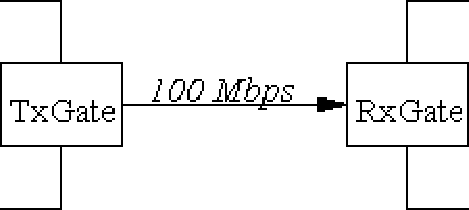
\includegraphics[width=2.315in, height=1.015in]{figures/usmanFig9}
    \caption{Connection with a data rate}
    \label{fig:ch-simple-modules:conn-w-data-rate}
  \end{center}
\end{figure}

While a message is under transmission, other messages have to wait
until the transmission finishes. You can still use \fname{send()}
while the gate is busy, but the message's arrival will be delayed;
just like the gate had an internal queue for the messages waiting to
be transmitted.


The {\opp} class library provides you with functions to check
whether a certain output gate is transmitting or to learn when
it finishes transmission.


If the connection with a data rate is not the immediate one connected
to the simple module's output gate but the second
one in the route, you have to check the second gate's busy
condition\index{gate!busy condition}.


\textbf{Implementation of message sending}


Message sending is implemented in the following way: the arrival
time\index{arrival time} and the bit error\index{bit error} flag of a
message are calculated at once, when the \fname{send()} (or similar)
function is invoked. That is, if the message travels through several
links until it reaches its destination, it is \textit{not} scheduled
individually for each link, but rather, every calculation is done
once, within the \fname{send()} call. This implementation was chosen
because of its run-time efficiency.

In the actual implementation of queuing the messages at busy gates and
modeling the transmission delay, messages do not actually queue up in
gates; gates do not have internal queues. Instead, as the time when
each gate will finish transmission is known at the time of sending the
message, the arrival time\index{arrival time} of the message can be
calculated in advance. Then the message will be stored in the event
queue (FES)\index{FES} until the simulation time advances to its
arrival time and it is retrieved by its destination module.

%
% TBD add pseudocode
%


\textbf{Consequence}


The implementation has the following consequence. If you change the
delay (or the bit error rate, or the data rate) of a link\index{link
  delay} during simulation, the modeling of messages sent ``just
before'' the parameter change will not be accurate. Namely, if link
parameters change while a message is ``under way'' in the model, that
message will not be affected by the parameter change, although it
should. However, all subsequent messages will be modelled correctly.
Similar for data rate: if a data rate changes during the simulation,
the change will affect only the messages that are \textit{sent} after
the change.

If it is important to model gates and channels with changing
properties, you can go two ways:
\begin{itemize}
  \item{write sender module such that they schedule events for when the
    gate finishes its current transmission and send then;}
  \item{alternatively, you can implement channels with
    simple modules (``active channels'').}
\end{itemize}

\textbf{The approach of some other simulators}


Note that some simulators (e.g. OPNET) assign \textit{packet queues}
to input gates (ports), and messages sent are buffered at the
destination module (or the remote end of the link) until received by
the destination module. With that approach, events and messages are
separate entities, that is, a \textit{send} operation includes placing
the message in the packet queue \textit{and} scheduling an event which
will signal the arrival of the packet. In some implementations, also
output gates have packet queues where packets wait until the channel
becomes free (available for transmission).

{\opp} gates\index{gate} don't have associated queues. The place
where the sent but not yet received messages are buffered is the
\textit{FES}\index{FES}.  {\opp}'s approach is potentially faster
than the above mentioned solution because it doesn't have the
enqueue/dequeue overhead and also spares an event creation. The
drawback is, as mentioned above, that changes to channel parameters do
not take effect immediately.





\section{Coding conventions}

Here's a bunch of advice on how to write {\opp} models. Some
of them are ``rules of thumb'', saying if you program like that,
you're likely to have less trouble; other conventions are aimed
at making the models produced by the {\opp} community more consistent.


Conventions for writing simple\index{module!simple} modules:
\index{module!conventions}
\begin{enumerate}
\item{Put the NED description, the C++ class declaration and the
    implementation into three separate files. Do not put two or more
    modules' code into the same file unless they are build upon one
    another - don't be afraid of small files! Thus, for a
    simple module called Foobar, you should have
    Foobar.ned, Foobar.h and Foobar.cc. This reduces coupling of
    module sources and makes your code more reusable.}
\item{Adopt a good coding style. Some hints: Choose your favourite
    indentation style and keep to that consistently. I recommend
    four-space indents and the brace placement style in which the
    {\opp} sources are written. Write only one statement per line.
    Avoid putting comments at the end of the line - place them
    \textit{above} the code on a separate line instead! Use blank
    lines to break the code into not-very-long logical blocks, and put
    a few-word comment above each block what that block does. Leave at
    least two blank lines between two (member) functions. The purpose
    of all that is that the structure of your code be obvious at the
    first glance!}
\item{Identifiers: Begin module type names with a capital letter, and
    capitalize the beginning of each word, like in TokenRingMAC.  Do
    not use underscore `\_` in module names. Use the C++-style naming
    on member functions: beginning of each word is capitalized (except
    for the first one) and no underscores: sendUnnumberedFrame().  On
    parameter names, you may use C-style (window\_size) or C++-style
    (windowSize) naming, whichever you prefer.}
\item{Make the functions virtual. Maybe someone who reuses your code
    will need a different behavior than what you thought of.}
\item{Use inheritance\index{inheritance} if you're writing a very complex
    simple module: create a basic
    simple module class and build upon it
    deriving new module classes. This will make your code more
    readable and easier to manage/reuse. Unfortunately, inheritance is
    not supported in NED so you actually have to make distinct NED
    descriptions for each simple module class.
    Even if you have an abstract classes, prepare a NED description
    for it: it is useful as a reference to others who might derive a
    different simple module class from your
    abstract class. Inheritance in NED\index{ned!inheritance} is
    planned in later releases of {\opp}.}
\item{Avoid global variables\index{global variables} (and what's the
    same, static class members).  They are not reset to their initial
    value (zero) when you run the simulation, stop it and rebuild the
    network. This can cause several problems when you use Cmdenv to
    execute several runs one after another, or in Tkenv when you
    rebuild the network from the menu.}
\item{Query the values of parameters into state variables
    (--\texttt{>}class members) of the \textit{same} name at the top
    of the \fname{activity()} function.  If you know the value of a
    parameter is a random value (like uniform 0..10) or it can change
    during simulation, then to avoid having to look it up by name each
    time (like \ttt{d=par(''delay'')}) you may query its pointer into a
    \cclass[cPar]{cPar*} state variable with the same name prepended with
    'p' (like \ttt{pDelay=\&par(''delay'')}).}
  \item{Use \fname{ev.printf()} and \texttt{ev <}\texttt{<}... (see
    later) to print out information on what the module is doing. Doing
    so will pay out several times when it comes to debugging. Use a
    parameter and a state variable called debug. Surround your
    debugging output (\texttt{ev <}\texttt{<}... and
    \fname{ev.printf()} calls) with \texttt{if(debug)}.  You may
    introduce more specific debug switches (like debug\_queuing etc.)}
\end{enumerate}




\section{Component libraries}

Because of the structure of the simulation system, one can create
libraries of reusable elements in several ways. The three basic
types are:
\begin{itemize}
\item{simple\index{module!simple} module libraries}
\item{NED source libraries}
\item{precompiled compound module libraries}
\end{itemize}

The elegant thing is that the user of the library does not need
to know which kind of library he/she is using; the three types
of libraries are equivalent in terms of usage.





\subsection{Simple module libraries}

Simple modules that can be used in more than one simulations can form an
object library\index{object library}. Good candidates for module
libraries\index{module!libraries} are simple\index{module!simple}
modules that implement:
\begin{itemize}
\item{Physical/Data-link protocols: Ethernet, Token Ring, FDDI, LAPB
    etc.}
\item{Higher layer protocols: IP, TCP, X.25 L2/L3, etc.}
\item{Network application types: E-mail, NFS, X, audio etc.}
\item{Basic elements: message generator, sink, concentrator/simple
    hub, queue etc.}
\item{Modules that implement routing algorithms in a multiprocessor or
    network}
\item{...}
\end{itemize}

To create a library, you compile the simple module C++ sources
and collect the object files in one directory. You'll also need
to the provide the NED descriptions:


\begin{Verbatim}[commandchars=\\\{\}]
library/generator.ned
generator.o
sink.ned
sink.o
ethernet.ned
ethernet.o
\end{Verbatim}



The NED files\index{ned!files} contain the interfaces of the
simple modules. For example:


\begin{Verbatim}[commandchars=\\\{\}]
// generator.ned
\textbf{simple} Generator
    \textbf{parameters}:
        interarrival time, message_length, message_kind;
    \textbf{gates}:
        \textbf{out}: output;
\textbf{endsimple}
\end{Verbatim}


The user of the library would include generator.ned in his/her
NED files, and link the executable with generator.o. This is
more or less the same concept as conventional C/C++ header files
and libraries. The basic advantage is the same as with C/C++:
you save compilation time and hide concrete implementation. The
latter also means that you can give the module library to others
without having to share the C++ source.


It could also be meaningful to provide the C++ header files with the
module class declarations. This would enable the user to directly call
the member functions of the module object from the simulation program
and derive new module classes by redefining the virtual functions.

You do not need to have a separate NED file for each module: you could
merge all of them into a single library.ned that contains the NED
declarations of all modules without all side effects.  However, it is
not recommended to put all object files into one library (.a or .lib),
because then every simple module would be present
in simulation programs linked with the library, regardless whether the
simulation uses them or not.



\subsection{Compound module NED source libraries}

\index{ned!libraries}

The NED sources of reusable compound\index{module!compound} modules
can also be placed in a library. Candidates are:
\begin{itemize}
\item{network nodes such as hubs, bridges, routers}
\item{different workstation/computer types: file server, X terminal
    etc.}
\item{node of a massively parallel multiprocessor (used in testing
    different topologies)}
\item{topology templates: parameterized ring, mesh, hypercube, torus
    etc. topologies, with the sizes (shapes etc) and the actual node
    types to be left as parameters}
\item{...}
\end{itemize}


The NED sources are used through the import\index{import files}
mechanism; the corresponding simple module object
files still to be linked in the executable.

The user does not necessarily notice that he/she is using a
compound module library and not a
simple module library. In NED files, the user
imports and uses the compound module sources in exactly the same way
as he/she used the simple module interface
declarations.  Linking also goes in the same way; if the
simple modules objects necessary for a certain
compound module are aggregated into a library (.a or .lib), the user
does not even notice the difference from the number of files he/she
has to link in.





\subsection{Precompiled compound module libraries}

\index{ned!libraries}

If you share a compound module with others, you do not necessarily
have to share the NED source and reveal the internals of the compound
module. You can turn the compound module into something that very much
looks like a simple module.


Suppose you have the following compound\index{module!compound} module:


\begin{Verbatim}[commandchars=\\\{\}]
// router-compound.ned
\textbf{module} Router:
    \textbf{parameters}:
        processing_delay, buffersize;
    \textbf{gates}:
        \textbf{in}: input_ports[];
        \textbf{out}: output_ports[];
    \textbf{submodules}:
        routing: RoutingModule
            \textbf{parameters}:
                //...
            \textbf{gatesizes}:
                //...
        datalink: DataLink[num_of_ports]
            \textbf{parameters}:
                retry_count = 5,
                window_size = 2;
                //...
    \textbf{connections}:
    //...
\textbf{endmodule}
\end{Verbatim}


First, you would compile this NED file with the NEDC compiler
and the resulting C++ code with the C++ compiler. Then you would
aggregate this object file with the simple module object files
into a single library (.a or .lib). Also, you would write a separate
NED file that declares the interface of the new ``simple''
module:


\begin{Verbatim}[commandchars=\\\{\}]
// router-simple.ned
\textbf{simple} Router:
    \textbf{parameters}:
        processing_delay, buffersize;
    \textbf{gates}:
        \textbf{in}: input_ports[];
        \textbf{out}: output_ports[];
\textbf{endsimple}
\end{Verbatim}



The method produced a \textit{precompiled compound
  module}\index{module!compound!precompiled}. The resulting two files
can be placed into a simple module library and
can be used identically to ordinary simple
modules.

Using precompiled compound\index{module!compound!precompiled} modules
you can hide the internal complexity of your model from direct
inspection. However, nothing can prevent a user from building a
simulation executable with it and exploring the structure of your
compound module using {\opp} simulation kernel
functions. Consequently, using precompiled
compound\index{module!compound!precompiled} modules is more useful as a
structuring tool.



\section{Some simulation techniques}

\subsection{Modeling computer networks}

The hierarchical module structure of {\opp} allows you to organize
the model around different levels:

Physical topology:
\begin{enumerate}
\item{Top-level network}
\item{Subnetwork (site)}
\item{LAN}
\item{node}
\end{enumerate}

Within a node:
\begin{enumerate}
\item{OSI layers. The Data-Link, Network, Transport, Application layers
are of greater importance.}
\item{Applications/protocols within a layer.}
\end{enumerate}

The advantage of {\opp} over many existing simulators is that the
depth of the module nesting\index{module!nesting depth} is not
limited, and, what is in connection with the previous one, that a
simple module can be transformed into a
compound\index{module!compound} module by splitting the code into
several simple\index{module!simple} modules \textit{without affecting
  existing users} of the module and vice versa. The latter means that
the programmer of the model is not under pressure from possibly
incorrect early design decisions about what to implement with a single
module and what with a compound\index{module!compound} module.



\subsection{Modeling multiprocessor systems}

One can make use of flexible model topologies. It is straightforward
to create ring, mesh, butterfly, torus, hypercube, tree, fat tree and
other topologies with conditional loop
connections\index{connection!loop}.


Furthermore, general \textit{topology
  templates}\index{topology!templates} (e.g. mesh or hypercube) can be
created, where the types of the actual nodes are left as parameters.
The actual node types are substituted as parameter values for each
concrete simulation. Topology templates could be placed in a library
and imported from there if needed.





\subsection{Parameter tuning}

Tuning means finding the parameter values which produce optimal
operation of the system. In {\opp}, you can tune the model during
runtime. The code that monitors performance and changes parameter
values can be placed:
\begin{itemize}
\item{inside the model. In this case, the code does not necessarily
    form separate module(s); you can add the extra code to any already
    existing module.}
\item{outside the model of the actual system. If you choose this
    method, you will create new modules that monitor and control the
    model.}
\end{itemize}

{\opp} supports the model tuning\index{model!tuning} concept by
providing reference parameters. Parameters that influence the model
performance and need to be tuned will be declared at the highest layer
and taken by both the model and the monitor part.


An example of model tuning is how one can determine the critical
throughput of a communication network by changing the offered
load according to performance measures of the network (queuing
times etc.)





\subsection{Multiple experiments within one simulation run}

One might need to perform a large number of simulation runs where
the model parameters are not known in advance. This can be the
case when one wants to optimize a system and parameter tuning
cannot be used because
\begin{enumerate}
\item{for each experiment, he wants to start the model from a
    well-defined initial state, or}
\item{he wants to change the model topology from one simulation run to
    the other}
\end{enumerate}

In this case, the following solution be followed. The network would
consist of only one simple module that would
organize the simulation runs by creating, running and destroying the
actual models with each experiment. The simple
module's code would look like this:


\begin{Verbatim}[commandchars=\\\{\}]
\textit{SimulationManager::activity()}
\{
    determine parameters for the first run
    while(true)
    \{
        create the model (a compound module) with the current
          run parameters schedule
        wait( some time) // while the model runs
        delete future events that belong to the model
        get statistics out of the model
        destroy the model
        if (simulation is done)
            break
        calculate parameters for the next run
    \}
    write out results
\}
\end{Verbatim}


The solutions built into {\opp} (flexible module topologies, dynamic
creation of compound modules etc.) strongly
support this concept.





\subsection{Dynamic topology optimization}

Dynamic topology optimization\index{topology!dynamic optimization} is
the generalization of the ``parameter tuning'' and ``multiple
experiments within one simulation run'' concepts. If one wants to
simulate large systems, it is possible that one part of the model
needs its topology to be optimized (optimal number of servers, optimal
interconnection etc.) while other parts of the model have reached
their steady state and should not be bothered.


This can be achieved by modifying the previous scheme. Parts
of the model that do not need topology optimization can be created
once and left running for the whole duration of the simulation;
other parts are examined and their structure is modified from
time to time.



%%% Local Variables:
%%% mode: latex
%%% TeX-master: "usman"
%%% End:

\cleardoublepage

\chapter{The Simulation Library}
\label{cha:the-simulation-library}

{\opp} has an extensive C++ class library which you can use when implementing
simple modules. Some areas of class librar have already been covered in the
previous chapters:

\begin{itemize}
  \item{events, messages, network packets: the \cclass{cMessage} and
    \cclass{cPacket} classes (chapter \ref{cha:messages})}
  \item{sending and receiving messages, scheduling and cancelling
    events, terminating the module or the simulation
    (section \ref{ch:simple-modules:sending-and-receiving})}
  \item{access to module gates and parameters via \cclass{cModule} member functions
    (sections \ref{ch:simple-modules:parameters} and \ref{ch:simple-modules:gates})}
  \item{accessing other modules in the network (section \ref{ch:simple-modules:walking-module-hieararchy})}
  \item{dynamic module creation (section \ref{ch:simple-modules:dynamic-module-creation})}
\end{itemize}

This chapter discusses the rest of the simulation library:

\begin{itemize}
  \item{random number generation: \fname{normal()},
    \fname{exponential()}, etc.}
  \item{module parameters: \cclass{cPar} class}
  \item{storing data in containers: \cclass{cArray},
    \cclass{cQueue}, \cclass{cBag} and
    \cclass{cLinkedList} classes}
  \item{routing support and discovery of network topology: \cclass{cTopology} class}
  \item{recording statistics into file: \cclass{cOutVector} class}
  \item{collecting simple statistics: \cclass{cStdDev} and
    \cclass{cWeightedStddev} classes}
  \item{distribution estimation: \cclass{cLongHistogram},
    \cclass{cDoubleHistogram}, \cclass{cVarHistogram}, \cclass{cPSquare},
    \cclass{cKSplit} classes}
  \item{making variables inspectable in the graphical user interface
    (Tkenv): the \fmac{WATCH()} macro (\cclass{cWatch} class)}
  \item{sending debug output to and prompting for user input in the graphical
    user interface (Tkenv\index{Tkenv}): the \ttt{ev}\index{ev} object (\cclass{cEnvir} class)}
\end{itemize}





\section{Class library conventions}

\subsubsection{Base class}
\label{sec:ch-sim-lib:cObject}


Classes in the {\opp} simulation library are derived from \cclass{cObject}.
Functionality and conventions that come from \cclass{cObject}:
\begin{itemize}
  \item{name attribute}
  \item{\fname{className()} member and other member functions giving textual
    information about the object}
  \item{conventions for assignment, copying, duplicating the object}
  \item{ownership\index{ownership} control for containers derived from \cclass{cObject}}
  \item{support for traversing the object tree}
  \item{support for inspecting the object in graphical user interfaces
    (Tkenv)}
  \item{support for automatic cleanup (garbage collection) at the end
    of the simulation}
\end{itemize}


Classes inherit and redefine several \cclass{cObject} member functions;
in the following we'll discuss some of the practically important
ones.


\subsubsection{Setting and getting attributes}


Member functions that set and query object attributes follow
consistent naming. The setter member function has the form setSomething(...)
and its getter counterpart is named something(), i.e. the ``get''
verb found in Java and some other libraries is omitted for brevity.
For example, the \textit{length} attribute of the \cclass{cMessage} class can
be set and read like this:

\begin{verbatim}
msg->setLength( 1024 );
length = msg->length();
\end{verbatim}


\subsubsection{className()}


For each class, the \fname{className()} member function returns the class
name as a string:

\begin{verbatim}
const char *classname = msg->className(); // returns "cMessage"
\end{verbatim}

\subsubsection{Name attribute}


An object can be assigned a name (a character string). The name
string is the first argument to the constructor of every class,
and it defaults to NULL (no name string). If you supply a name
string, the object will make its own copy (\fname{strdup()}). As an example,
you can create a message object like this:

\begin{verbatim}
cMessage *mymsg = new cMessage("mymsg");
\end{verbatim}


You can also set the name after the object has been created:

\begin{verbatim}
mymsg->setName("mymsg");
\end{verbatim}

You can get a pointer to the internally stored copy of the name
string like this:

\begin{verbatim}
const char *name = mymsg->name(); // --> returns ptr to internal copy
                                  // of "mymsg"
\end{verbatim}


For convenience and efficiency reasons, the empty string ``''
and NULL are treated as equivalent by library objects: ``''
is stored as NULL (so that it does not consume heap), but it
is returned as ``'' (so that it is easier to print
out etc). Thus, if you create a message object with either NULL
or ``'' as name, it will be stored as NULL and \fname{name()}
will return a pointer to ``'', a static string:

\begin{verbatim}
cMessage *msg = new cMessage(NULL, <additional args>);
const char *str = msg->name(); // --> returns ptr to  ""
\end{verbatim}


\subsubsection{fullName() and fullPath()}


Objects have two more member functions which return other sort
of names based on the name attribute: \fname{fullName()} and \fname{fullPath()}.

Suppose we have a module in the network university\_lan, compound
module fddi\_ring, simple module station[10]. If you call the functions
on the simple module object (\cclass{cSimpleModule} inherits from
\cclass{cObject}, too), the functions will return these values:

\begin{verbatim}
ev << module->name(); // --> "station"
ev << module->fullName(); // --> "station[10]"
ev << module->fullPath(); // --> "university_lan.fddi_ring.station[10]"
\end{verbatim}



These functions work for any object. For example, a local object
inside the module would produce results like this:


\begin{verbatim}
void FDDIStation::activity()
{
    cQueue buffer("buffer");
    ev << buffer->fullPath(); // --> "university_lan.fddi_ring.
                              // station[10].buffer"
}
\end{verbatim}



\fname{fullName()} and \fname{fullPath()}, together with
\fname{className()} can be used for example to generate informative
error messages.

Be aware that \fname{fullName()} and \fname{fullPath()} return
pointers to static buffers. Each call will overwrite the previous
content of the buffer, so for example you shouldn't put two calls in a
single \fname{printf()} statement:

\begin{verbatim}
ev.printf("object1 is '%s', object2 is '%s'\n",
          object1->fullPath(),
          object2->fullPath()
         ); // WRONG! Same string is printed twice!!!
\end{verbatim}


\subsubsection{Copying and duplicating objects}


The \fname{dup()} member function creates an exact copy of the
object\index{object!copy}, duplicating\index{object!duplication}
contained objects also if necessary. This is especially useful in the
case of message objects. \fname{dup()} returns a pointer of type
\cclass[cObject]{cObject*}, so it needs to be cast to the proper type:

\begin{verbatim}
cMessage *copyMsg = (cMessage *) msg->dup();
\end{verbatim}


\fname{dup()} works through calling the copy constructor, which in
turn relies on the assignment operator between objects.
\fname{operator=()} can be used to copy contents of an object into
another object of the same type. The copying is done properly; object
contained in the object will also be duplicated if necessary. For
various reasons, \fname{operator=()} does not copy the name string;
the copy constructor\index{copy constructor} does it.


\subsubsection{Iterators}


There are several container classes in the library (\cclass{cQueue},
\cclass{cArray} etc.) For many of them, there is a corresponding
iterator class that you can use to loop through the objects stored in
the container.

For example:

\begin{verbatim}
cQueue queue;

//..
for (cQueue::Iterator queueIter(queue); !queueIter.end(); queueIter++)
{
    cObject *containedObject = queueIter();
}
\end{verbatim}


\subsubsection{Ownership control}


By default, if a container object is destroyed, it destroys the
contained objects too. If you call \fname{dup()}, the contained
objects are duplicated too for the new container. This is done so
because contained objects are owned by the container; ownership is
defined as the right/duty of deallocation. However, there is a
fine-grain ownership control\index{ownership} mechanism built
in which allows you to specify on per-object basis whether you want
objects to be owned by the container or not; by calling the
\fname{takeOwnership()} member function with false, you tell the
container that you don't want it to become the owner of objects that
will be inserted in the future.

The ownership mechanism is discussed in detail in section
\ref{sec:ch-sim-lib:ownership-management}


\section{Utilities}

\subsubsection{Tracing}


The tracing feature will be used extensively in the code examples,
so it is shortly introduced here. It will be covered in detail
in a later section.

The \ttt{ev}\index{ev} object represents the user interface of the
simulation.  You can send debugging output to \ttt{ev} with the C++-style
output operators:

\begin{verbatim}
ev << "packet received, sequence number is "
   << seq_num << endl;
\end{verbatim}

An alternative solution is \fname{ev.printf()}:

\begin{verbatim}
ev.printf("packet received, sequence number is %d\n", seq_num);
\end{verbatim}

\subsubsection{Simulation time conversion}


There are utility functions which convert simulation
time\index{simulation time} (\cclass{simtime\_t}) to a printable string
(like \ttt{"3s 130ms 230us"}) and vica versa.


The \fname{simtimeToStr()} function converts a \cclass{simtime\_t}
(passed in the first arg) to textual form. The result is placed into
the buffer pointed to by the second arg. If the second arg is omitted
or it is NULL, \fname{simtimeToStr()} will place the result into a
static buffer which is overwritten with each call:

\begin{verbatim}
char buf[32];
ev.printf("t1=%s, t2=%s\n", simtimeToStr(t1), simTimeToStr(t2,buf));
\end{verbatim}


The \fname{strToSimtime()} function parses a time specification passed
in a string, and returns a \cclass{simtime\_t}. If the string cannot
be entirely interpreted, -1 is returned.

\begin{verbatim}
simtime_t t = strToSimtime("30s 152ms");
\end{verbatim}

Another variant, \fname{strToSimtime0()} can be used if the time
string is a substring in a larger string. Instead of taking a char*,
it takes a reference to char* (char*\&) as the first argument.  The
function sets the pointer to the first character that could not be
interpreted as part of the time string, and returns the value. It
never returns -1; if nothing at the beginning of the string looked
like simulation time, it returns 0.

\begin{verbatim}
const char *s = "30s 152ms and some rubbish";

simtime_t t = strToSimtime0(s); // now s points to "and some rubbish"
\end{verbatim}

\subsubsection{Utility \texttt{<string.h>} functions}

\begin{sloppypar}
The \fname{opp\_strdup()}, \fname{opp\_strcpy()}, \fname{opp\_strcmp()}
functions are the same as their \texttt{<string.h>} equivalents,
except that they treat NULL and the empty string (\ttt{""}) as identical,
and \fname{opp\_str\-dup()} uses operator new instead of \fname{malloc()}.
\end{sloppypar}

The \fname{opp\_concat()} function might also be useful, for example
in constructing object names. It takes up to four \ttt{const char *}
pointers, concatenates them in a static buffer and returns a pointer
to the result. The result's length shouldn't exceed 255 characters.



\section{Generating random numbers}

Random numbers in simulation are never random. Rather, they are
produced using deteministic algorithms. Algorithms take a \textit{seed} value
and perform some deterministic calculations on them to produce
a ``random'' number and the next seed. Such algorithms and their
implementations are called \textit{random number generators} or RNGs,
or sometimes pseudo random number generators or PRNGs to highlight
their deterministic nature.
  \footnote{There exist real random numbers too, see e.g.
  http://www.random.org/, http://www.comscire.com, or the Linux
  /dev/random device.}

Starting from the same seed, RNGs always produce the same sequence
of random numbers. This is a useful property and of great importance,
because it makes simulation runs repeatable.

RNGs produce uniformly distributed integers in some range,
usually between 0 or 1 and $2^{32}$ or so. Matematical transformations
are used to produce random variates from them that correspond to
specific distributions.

\subsection{Random number generators}

\subsubsection{The current RNG}

The currently used random number generator in {\opp} is
a linear congruential generator\index{linear congruential generator}
(LCG) with a cycle length of $2^{31}-2$.
The startup code of {\opp} contains code that checks if the random number
generator works OK, so you do not have to worry about this if you port
the simulator to a new architecture or use a different compiler.

The random number generator was taken from \cite{Jain91}, pp. 441-444,455.
It has the following properties:
\begin{itemize}
   \item{Range: $1... 2^{31}-2$}
   \item{Period length: $2^{31}-2$}
   \item{Method: $x := (x * 7^{5}) mod (2^{31}-1)$}
   \item{Verification: if $x[0] = 1$ then $x[10000] = 1,043,618,065$ }
   \item{Required hardware: exactly 32-bit integer arithmetics}
\end{itemize}

The concrete implementation:

\begin{verbatim}
long intrand()
{
  const long int a=16807, q=127773, r=2836;
  seed=a*(seed%q) - r*(seed/q);
  if (seed<=0) seed+=INTRAND_MAX;
  return seed;
}
\end{verbatim}


\subsubsection{Caution!}

The above ``minimal standard'' RNG is only suitable for small-scale
simulation studies. As shown by Karl Entacher et al. in \cite{Entacher02},
the cycle length of about $2^{31}$ is too small (on todays
fast computers it is easy to exhaust all random numbers), and
the structure of the generated ``random'' points is too regular.
The \cite{Hellekalek98} paper gives you a broader overview of issues
associated with RNGs used for simulation, and it's well worth reading.
It also gives you useful links and references to further reading
on the topic.

Work is underway to create a flexible and extensible
random number architecture in future versions of {\opp},
and to integrate modern RNGs such as L'Ecuyer's CMRG \cite{LEcuyer02}
with a period of about $2^{191}$ and/or
Mersenne Twister \cite{Matsumoto98}.


\subsubsection{Multiple RNGs}

If a simulation program uses random numbers for more than one purpose,
the numbers should come from different random number generators.
{\opp} provides several independent random number generators (by
default 32; this number is \#defined as
\fmac{NUM\_RANDOM\_GENE\-RATORS} in \ttt{utils.h}).

To avoid unwanted correlation, it is also important that different
simulation runs and different random number sources within one
simulation run use non-overlapping series of random numbers,
so the generators should be started with seeds well apart. For
selecting good seeds, the seedtool\index{seedtool} program can be used (it is
documented later).


\subsubsection{Accessing RNGs}

Integers can be generated via the \fname{intrand()} function:

\begin{verbatim}
long rnd = intrand();   // in the range 1..INTRAND_MAX-1
\end{verbatim}

The random number seed can be specified in the ini file
(\fpar[random-seed]{random-seed=}) or set directly from within
simple modules with the \fname{randseed()}
function:

\begin{verbatim}
randseed( 10 );         // set seed to 10
long seed = randseed(); // current seed value
\end{verbatim}

Zero is not allowed as a seed.

The \fname{intrand()} and \fname{randseed()} functions use generator 0. They have
another variant which uses a specified generator:

\begin{verbatim}
long rnd = genk_intrand(6); // like intrand(), using generator 6
genk_randseed( k, 167 );    // set seed of generator k to 167
\end{verbatim}


The \fname[intrand()]{intrand(n)} and \fname{dblrand()} functions are based on \fname{intrand()}:

\begin{verbatim}
int dice = 1 + intrand(6); // result of intrand(6) is in the range 0..5
                           // (it is calculated as intrand()%6)

double prob = dblrand();   // dblrand() produces numbers in [0,1)
                           // calculated as
                           // intrand()/(double)INTRAND_MAX
\end{verbatim}


They also have their counterparts that use generator \textit{k}:

\begin{verbatim}
int dice = 1 + genk_intrand(k,6); // uses generator k
double prob = genk_dblrand(k);    // ""
\end{verbatim}




\subsection{Random variates}

The following functions are based on \fname{dblrand()} and return
random variables of different distributions\index{distribution!random variables}\index{random!numbers from distributions}:

Random variate functions use one of the random number generators (RNGs)
provided by \opp. By default this is generator 0, but you can specify
which one to be used.

{\opp} has the following predefined distributions\index{distribution!predefined}:

\begin{longtable}{|p{6.5cm}|p{7.5cm}|}
\hline
\tbf{Function} & \tbf{Description}\\\hline
\multicolumn{2}{|c|}{\tbf{Continuous distributions}}\\\hline
\fname{uniform(a, b, \textit{rng=0})} & uniform distribution in the range [a,b) \\\hline
\fname{exponential(mean, \textit{rng=0})} & exponential distribution with the given mean \\\hline
\fname{normal(mean, stddev, \textit{rng=0})} & normal distribution with the given mean and standard deviation \\\hline
\fname{truncnormal(mean, stddev, \textit{rng=0})} & normal distribution truncated to nonnegative values \\\hline
\fname{gamma\_d(alpha, beta, \textit{rng=0})} & gamma distribution with parameters alpha>0, beta>0 \\\hline
\fname{beta(alpha1, alpha2, \textit{rng=0})} & beta distribution with parameters alpha1>0, alpha2>0 \\\hline
\fname{erlang\_k(k, mean, \textit{rng=0})} & Erlang distribution with k>0 phases and the given mean \\\hline
\fname{chi\_square(k, \textit{rng=0})} & chi-square distribution with k>0 degrees of freedom \\\hline
\fname{student\_t(i, \textit{rng=0})} & student-t distribution with i>0 degrees of freedom \\\hline
\fname{cauchy(a, b, \textit{rng=0})} & Cauchy distribution with parameters a,b where b>0 \\\hline
\fname{triang(a, b, c, \textit{rng=0})} & triangular distribution with parameters a<=b<=c, a!=c \\\hline
\fname{lognormal(m, s, rng=0)} & lognormal distribution with mean m and variance s>0 \\\hline
\fname{weibull(a, b, \textit{rng=0})} & Weibull distribution with parameters a>0, b>0 \\\hline
\fname{pareto\_shifted(a, b, c, \textit{rng=0})} & generalized Pareto distribution with parameters a, b and shift c \\\hline
\multicolumn{2}{|c|}{\tbf{Discrete distributions}} \\\hline
\fname{intuniform(a, b, \textit{rng=0})} & uniform integer from a..b \\\hline
\fname{bernoulli(p, \textit{rng=0})} & result of a Bernoulli trial with probability 0<=p<=1 (1 with probability p and 0 with probability (1-p)) \\\hline
\fname{binomial(n, p, \textit{rng=0})} & binomial distribution with parameters n>=0 and 0<=p<=1 \\\hline
\fname{geometric(p, \textit{rng=0})} & geometric distribution with parameter 0<=p<=1 \\\hline
\fname{negbinomial(n, p, \textit{rng=0})} & binomial distribution with parameters n>0 and 0<=p<=1\\\hline
\fname{poisson(lambda, \textit{rng=0})} & Poisson distribution with parameter lambda \\\hline

\end{longtable}


They are the same functions that can be used in NED files.
\fname{intuniform()} generates integers including both the lower and
upper limit, so for example the outcome of tossing a coin could be
written as intuniform(1,2).  \fname{truncnormal()} is the normal
distribution truncated to nonnegative values; its implementation
generates a number with normal distribution and if the result is
negative, it keeps generating other numbers until the outcome is
nonnegative.

If the above distributions do not suffice, you can write your own
functions\index{distribution!custom}. If you register your functions
with the \fmac{Register\_Function()} macro, you can use them in NED
files and ini files too.


\subsection{Random numbers from histograms}

You can also specify your distribution as a
histogram\index{distribution!as histogram}. The
\cclass{cLongHistogram}, \cclass{cDoubleHistogram},
\cclass{cVarHistogram}, \cclass{cKSplit} or \cclass{cPSquare} classes
are there to generate random numbers from equi\-dis\-tant-cell or
equiprobable-cell histograms.  This feature is documented later, with
the statistical classes.





\section{Container classes}

\subsection{Queue class: cQueue}

\subsubsection{Basic usage}


\cclass{cQueue} is a container class that acts as a queue.
\cclass{cQueue} can hold objects of type derived from \cclass{cObject}
(almost all classes from the {\opp} library), such as
\cclass{cMessage}, \cclass{cPar}, etc. Internally, \cclass{cQueue}
uses a double-linked list to store the elements.

A queue object has a head and a tail. Normally, new elements
are inserted at its head and elements are removed at its tail.


\begin{figure}[htbp]
  \begin{center}
    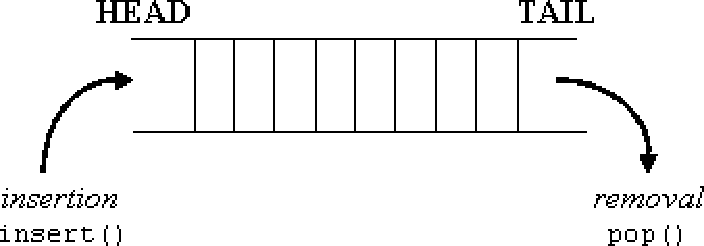
\includegraphics[width=3.703in, height=1.303in]{figures/usmanFig10}
    \caption{What is what with cQueue}
    \label{fig:ch-sim-lib:cqueue}
  \end{center}
\end{figure}

The basic \cclass{cQueue} member functions dealing with insertion and removal
are \fname{insert()} and \fname{pop()}. They are used
like this:

\begin{verbatim}
cQueue queue("my-queue");
cMessage *msg;

// insert messages
for (int i=0; i<10; i++)
{
  msg = new cMessage;
  queue.insert( msg );
}

// remove messages
while( ! queue.empty() )
{
  msg = (cMessage *)queue.pop();
  delete msg;
}
\end{verbatim}


The \fname{length()} member function returns the number of items in the
queue, and \fname{empty()} tells whether there's anything in the queue.

There are other functions dealing with insertion and removal.  The
\fname{insertBefore()} and \fname{insertAfter()} functions insert a
new item exactly before and after a specified one, regardless of the
ordering function.

The \fname{tail()} and \fname{head()} functions return pointers to the objects
at the tail and head of the queue, without affecting queue contents.



The \fname{pop()} function can be used to remove items from the
tail of the queue, and the \fname{remove()} function can be
used to remove any item known by its pointer from the queue:


\fname[queue.remove()]{queue.remove( msg );}



\subsubsection{Priority queue}


By default, \cclass{cQueue} implements a FIFO, but it can also act as
a priority queue, that is, it can keep the inserted objects
ordered\index{queue!order}.  If you want to use this feature, you have
to provide a function that takes two \cclass{cObject} pointers,
compares the two objects and returns -1, 0 or 1 as the result (see the
reference for details).  An example of setting up an ordered
\cclass{cQueue}:

\begin{verbatim}
cQueue sortedqueue("sortedqueue", cObject::cmpbyname, true );
                        // sorted by object name, ascending
\end{verbatim}


If the queue object is set up as an ordered queue, the \fname{insert()}
function uses the ordering function: it searches the queue contents
from the head until it reaches the position where the new item
needs to be inserted, and inserts it there.


\subsubsection{Iterators}


Normally, you can only access the objects at the head or tail of the
queue. However, if you use an iterator class, \cclass{cQueue::Iterator},
you can examine each object in the queue\index{queue!iteration}.

The \cclass{cQueue::Iterator} constructor takes two arguments, the first
is the queue object and the second one specifies the initial position
of the iterator: 0=tail, 1=head. Otherwise it acts as any other
{\opp} iterator class: you can use the ++ and -- operators to advance
it, the () operator to get a pointer to the current item, and the
\fname{end()} member function to examine if you're at the end (or the
beginning) of the queue.


An example:

\begin{verbatim}
for( cQueue::Iterator iter(queue,1); !iter.end(), iter++)
{
  cMessage *msg = (cMessage *) iter();
  //...
}
\end{verbatim}




\subsection{Expandable array: cArray}

\subsubsection{Basic usage}


\cclass{cArray} is a container class that holds objects derived from
\cclass{cObject}. \cclass{cArray} stores the pointers of the objects
inserted instead of making copies. \cclass{cArray} works as an array,
but if it gets full, it grows automatically. Internally,
\cclass{cArray} is implemented with an array of pointers; if the array
gets full, it is reallocated.

\cclass{cArray} objects are used in {\opp} to store parameters
attached to messages, and internally, for storing module parameters
and gates.


Creating an array:

\begin{verbatim}
cArray array("array");
\end{verbatim}

Adding an object at the first free index:

\begin{verbatim}
cPar *p = new cPar("par");
int index = array.add( p );
\end{verbatim}


Adding an object at a given index (if the index is occupied,
you'll get an error message):

\begin{verbatim}
cPar *p = new cPar("par");
int index = array.addAt(5,p);
\end{verbatim}


Finding an object in the array:

\begin{verbatim}
int index = array.find(p);
\end{verbatim}

Getting a pointer to an object at a given index:

\begin{verbatim}
cPar *p = (cPar *) array[index];
\end{verbatim}

You can also search the array or get a pointer to an object by
the object's name:

\begin{verbatim}
int index = array.find("par");
Par *p = (cPar *) array["par"];
\end{verbatim}


You can remove an object from the array by calling \fname{remove()}
with the object name, the index position or the object pointer:

\begin{verbatim}
array.remove("par");
array.remove(index);
array.remove( p );
\end{verbatim}


The \fname{remove()} function doesn't deallocate the object, but it
returns the object pointer. If you also want to deallocate it, you can
write:

\begin{verbatim}
delete array.remove( index );
\end{verbatim}

\subsubsection{Iteration}


\cclass{cArray} has no iterator, but it's easy to loop through all the
indices with an integer variable. The \fname{items()} member function
returns the largest index plus one.

\begin{verbatim}
for (int i=0; i<array.items(); i++)
{
  if (array[i]) // is this position used?
  {
    cObject *obj = array[i];
    ev << obj->name() << endl;
  }
}
\end{verbatim}




\section{Non-object container classes}

There are two container classes to store non-object
items\index{non-object container}: \cclass{cLinkedList} and
\cclass{cBag}.  The first one parallels with \cclass{cQueue}, the
second one with \cclass{cArray}. They can be useful if you have to
deal with C structs or objects that are not derived from
\cclass{cObject}.

See the class library reference for more info about them.





\section{The parameter class: cPar}

\subsection{Basic usage}

\cclass{cPar} is a class that is designed to hold a value. The value
is numeric (long or double) in the first place, but string, pointer
and other types are also supported.

cPar is used in {\opp} in the following places:

\begin{itemize}
  \item{as module parameters}
  \item{as message parameters}
\end{itemize}

There are many ways to set a \cclass{cPar}'s value. One is the set...Value()
member functions:

\begin{verbatim}
cPar pp("pp");
pp.setDoubleValue(1.0);
\end{verbatim}


or by using overloaded operators:

\begin{verbatim}
cPar pp("pp");
pp = 1.0;
\end{verbatim}


For reading its value, it is best to use overloaded type cast
operators:

\begin{verbatim}
double d1 = (double)pp;
// or simply:
double d2 = pp;
\end{verbatim}

Long integers:

\begin{verbatim}
pp = 89363L; // or:
pp.setLongValue( 89363L );
\end{verbatim}

Character string:

\begin{verbatim}
pp = "hi there"; // or:
pp.setStringValue( "hi there" );
\end{verbatim}


The \cclass{cPar} object makes its own copy of the string, so the
original one does not need to be preserved. Short strings (less than
\ensuremath{\sim}20 chars) are handled more efficiently because they
are stored in the object's memory space (and are not dynamically
allocated).

There are several other types \cclass{cPar} can store: such as boolean,
void* pointer; cObject* pointer,  function with constant args;
they will be mentioned in the next section.

For numeric and string types, an input flag\index{input flag} can be
set. In this case, when the object's value is first used, the
parameter value will be searched for in the configuration (ini)
file\index{ini file}; if it is not found there, the user will be given
a chance to enter the value interactively.


Examples:

\begin{verbatim}
cPar inp("inp");
inp.setPrompt("Enter my value:");
inp.setInput( true );   // make it an input parameter
double a = (double)inp; // the user will be prompted HERE
\end{verbatim}




\subsection{Random number generation through cPar}

Setting \cclass{cPar} to call a function with constant arguments can
be used to make \cclass{cPar} return random variables\index{random!variables} of different distributions\index{distribution}:

\begin{verbatim}
cPar rnd("rnd");
rnd.setDoubleValue(intuniform, -10.0, 10.0);// uniform distr.
rnd.setDoubleValue(normal, 100.0, 5.0); // normal distr. (mean,dev)
rnd.setDoubleValue(exponential, 10.0); // exponential distr. (mean)
\end{verbatim}

\fname{intuniform()}, \fname{normal()} etc. are ordinary C functions
taking double arguments and returning double. Each time you read the
value of a \cclass{cPar} containing a function like above, the
function will be called with the given constant arguments (e.g.
normal(100.0,5.0)) and its return value used.


The above functions use number 0 from the several random number
generators. To use another generator, use the genk\_xxx versions
of the random functions:

\begin{verbatim}
rnd.setDoubleValue(genk\_normal, 3, 100.0, 5.0); // uses generator 3
\end{verbatim}

A \cclass{cPar} object can also be set to return a random variable from
a distribution collected by a statistical data collection object:

\begin{verbatim}
cDoubleHistogram hist =....; // the distribution
cPar rnd2("rnd2");
rnd2.setDoubleValue(hist);
\end{verbatim}




\subsection{Storing object and non-object pointers in cPar}

\cclass{cPar} can store pointers to {\opp} objects. You can use both
assignment and the \fname{setObjectValue()} member function:

\begin{verbatim}
cQueue *queue = new cQueue("queue"); // just an example
cPar par1, par2;
par1 = (cObject *) queue;
par2.setObjectValue( queue );
\end{verbatim}

To get the store pointer back, you can use typecast or the \fname{objectValue()}
member function:

\begin{verbatim}
cQueue *q1 = (cQueue *)(cObject *)par1;
cQueue *q2 = (cQueue *)par2.objectValue();
\end{verbatim}


Whether the \cclass{cPar} object will own the other object or not is
controlled by the \fname{takeOwnership()}\index{ownership} member
function, just as with container classes. This is documented in detail
in the class library reference.  By default, \cclass{cPar} will own
the object.

\cclass{cPar} can be used to store non-object
pointers\index{non-object pointers} (for example C structs) or
non-{\opp} object types in the parameter object.  It works very
similarly to the above mechanism. An example:

\begin{verbatim}
double *mem = new double[15];
cPar par1, par2;
par1 = (void *) mem;
par2.setPointerValue( (void *)mem );
...
double *m1 = (double *)(void *)par1;
double *m2 = (double *)par2.pointerValue();
\end{verbatim}


Memory management\index{cPar memory management} can be specified by
\cclass{cPar}'s \fname{configPointer()} member function. It takes
three arguments: a pointer to a user-supplied deallocation
function, a pointer to a user-supplied duplication function and
an item size. If all three are 0 (NULL), no memory management is done,
that is, the pointer is treated as a mere pointer. This is the default
behaviour. If you supply only the item size (and both function
pointers are NULL), \cclass{cPar} will use the delete operator to
deallocate the memory area when the \cclass{cPar} object is
destructed, and it will use new char[size] followed by a
\fname{memcpy()} to duplicate the memory area whenever the
\cclass{cPar} object is duplicated. If you need more sophisticated
memory management, you can supply your own deallocation and
duplication functions.

An example for simple memory management:

\begin{verbatim}
double *mem = new double[15];
cPar par;
par.setPointerValue((void *) mem);
par.configPointer(NULL, NULL, 15*sizeof(double));
// -> now if par goes out of scope, it will delete the 15-double array.
\end{verbatim}

The \fname{configPointer()} setting only affects what happens when the
\cclass{cPar} is deleted, duplicated or copied, but does \textit{not}
apply to assigning new pointers. That is, if \textit{you} assign a new
void* to the \cclass{cPar}, you simply overwrite the pointer -- the
block denoted by the old pointer is \textit{not} deleted. This fact
can be used to extract some dynamically allocated block out of the
\cclass{cPar}: carrying on the previous example, you would extract the
array of 15 doubles from the \cclass{cPar} like this:

\begin{verbatim}
double *mem2 = (double *)par.pointerValue();
par.setValue( (void *)0 );
// -> now par has nothing to do with the double[15] array
\end{verbatim}



However, if you assign some non-pointer value\index{non-pointer value}
to the \cclass{cPar}, beware: this \textit{will} activate the memory
management for the block. If you temporarily use the same
\cclass{cPar} object to store other than void* ('P') values, the
\fname{configPointer()} setting is lost.



\subsection{Reverse Polish expressions}

This feature is rarely needed by the user, it is more used internally.
A \cclass{cPar} object can also store
expressions\index{cPar!expressions}. In this case, the expression must
be given in reversed Polish form\index{reversed polish notation}. An
example:

\begin{verbatim}
cPar::XElem *expression = new cPar::XElem[5];
expression[0] = &par("count"); // pointer to
module parameter
expression[1] = 1;
expression[2] = '+';
expression[3] = 2;
expression[4] = '/';

cPar expr("expr");
expr.setDoubleValue(expression,5);
\end{verbatim}


The \cclass{cPar} object created above contains the $(count+1)/2$
expression where \textit{count} is a module parameter. Each time the
\cclass{cPar} is evaluated, it recalculates the expression, using the
current value of count. Note the \& sign in front of
\texttt{par(''count'')} expression: if it was not there, the parameter
would be taken by value\index{parameter!by value}, evaluated once and
then the resulting constant would be used.

Another example is a distribution\index{distribution} with mean and
standard deviation given by module parameters:

\begin{verbatim}
cPar::XElem *expression = new cPar::XElem[3];
expression[0] = &par("mean");
expression[1] = &par("stddev");
expression[2] = normal; // pointer to the normal(double,double) func.

cPar expr("expr");
expr.setDoubleValue(expression,3);
\end{verbatim}


For more information, see the reference and the code NEDC generates
for parameter expressions\index{parameter!expressions}.



\subsection{Using redirection}

A \cclass{cPar} object can be set to stand for a value actually stored
in another \cclass{cPar} object. This is called \textit{indirect} or
\textit{redirected} value. When using redirection\index{redirection},
every operation on the value (i.e.  reading or changing it) will be
actually done to the other \cclass{cPar} object:

\begin{figure}[htbp]
  \begin{center}
    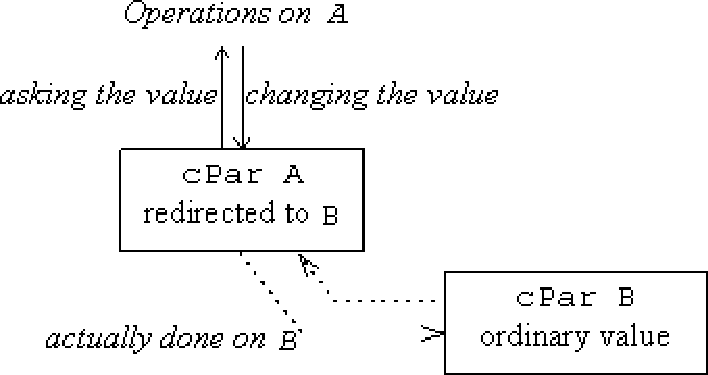
\includegraphics[width=3.608in, height=1.908in]{figures/usmanFig11}
    \caption{cPar redirection}
    \label{fig:ch-sim-lib:cPar-redirection}
  \end{center}
\end{figure}

Redirection is how module parameters taken by
reference\index{module!parameters!by reference} are implemented.  The
redirection does not include name strings. That is, if you say
A-\texttt{>}setName(''newname'') in the above example, A's name will
be changed as the name member is not redirected. (This is natural if
you consider parameters taken by reference: a parameter should/can
have different name than the value it refers to.)


You create a redirection with the \fname{setRedirection()} function:

\begin{verbatim}
cPar *bb = new cPar("bb"); // background value
bb = 10L;
cPar a("a"); // we'll redirect this object

a.setRedirection(bb); // create redirection
\end{verbatim}


Now every operation you do on a's value will be done to bb:

\begin{verbatim}
long x = a; // returns bb's value, 10L
a = 5;      // bb's value changes to 5
\end{verbatim}


The only way to determine whether a is really holding the value or it
is redirected to another \cclass{cPar} is to use the
\fname{isRedirected()} member function which returns a bool, or
\fname{redirection()} which returns the pointer to the background
object, or NULL if there's no redirection:

\begin{verbatim}
cPar *redir = a.redirection(); // returns bb's pointer
if (redir != NULL)
  ev << "a is redirected to " << redir->name() << endl;
\end{verbatim}


To break the link between the two objects, use the
\fname{cancelRedirection()} member function. (No other method will
work, including assigning a the value of another \cclass{cPar}
object.) The \fname{cancelRedirection()} function gives the \texttt{(long)0}
value to the redirected object (the other will be unaffected). If you
want to cancel the indirection but keep the old value, you can do
something like this:

\begin{verbatim}
cPar *value = a.redirection();  // bb's pointer
a.cancelRedirection();          // break the link; value of a is now 0
a = *value;                     // copy the contents of bb into a
\end{verbatim}




\subsection{Type characters}

Internally, \cclass{cPar} objects identify the types of the stored values
by type characters. The type character\index{type character} is returned by the \fname{type()}
member function:

\begin{verbatim}
cPar par = 10L;
char typechar = par.type(); // returns 'L'
\end{verbatim}

The full table of type characters is presented in the \textit{Summary}
section below.

The \fname{isNumeric()} function tells whether the object
stores one of the numeric types, so that e.g. \fname{asDoubleValue()}
can be invoked on it.




\subsection{Summary}

The various \cclass{cPar} types and the member functions\index{cPar
  types and member functions} used to manipulate them are summarized
in the following table:

\begin{longtable}{|p{0.7cm}|p{1.2cm}|p{5.2cm}|p{6cm}|}
\hline
% ROW 1
\tabheadcol
\textbf{Type\linebreak
char} &
\textbf{Type \linebreak
name} &
\textbf{Member functions} &
\textbf{Description}\\
\hline
%% ROW 2
S &  string &
\ttt{setStringValue( \linebreak
\hspace*{0.3cm}  const char *); \linebreak
const char * \linebreak
\hspace*{0.3cm} \fname{stringValue()}; \linebreak
op const char *(); \linebreak
op=(const char *);} &
{\raggedright
string value. Short strings (len\texttt{<}=27) are stored inside
\cclass{cPar} object, without using heap allocation.}\\\hline
%% ROW 3
B &  boolean &
\ttt{setBoolValue(bool); \linebreak
bool \fname{boolValue()}; \linebreak
op \fname{bool()}; \linebreak
op=(bool);} &
boolean value. Can also be retrieved from the object as long  (0 or 1).\\\hline
%% ROW 4
L & long int &
\ttt{setLongValue(long); \linebreak
long \fname{longValue()}; \linebreak
op \fname{long()}; \linebreak
op=(long);} &
signed long integer value. Can also be retrieved from the object
as double.\\\hline
%% ROW 5
D & double &
\ttt{setDoubleValue(double); \linebreak
double \fname{doubleValue()}; \linebreak
op \fname{double()}; \linebreak
op=(double);} &
double-precision floating point value.\\\hline
%% ROW 6
F & function &
\ttt{setDoubleValue( \linebreak
\hspace*{0.3cm} MathFunc, \linebreak
\hspace*{0.3cm} [double], \linebreak
\hspace*{0.3cm} [double], \linebreak
\hspace*{0.3cm} [double]); \linebreak
double \fname{doubleValue()}; \linebreak
op \fname{double()}; \linebreak
} &
Mathematical function with constant arguments. The function
is given by its pointer; it must take 0,1,2 or 3 doubles and
return a double. This type is mainly used to generate random
numbers: e.g. the function takes mean and standard deviation
and returns random variable of a certain distribution.\\\hline
%% ROW 7
X & expr. &
\ttt{setDoubleValue( \linebreak
\hspace*{0.3cm} cPar::XElem*,int); \linebreak
double \fname{doubleValue()}; \linebreak
op \fname{double()};}
&
Reverse Polish expression. Expression can contain constants,
\cclass{cPar} objects, refer to other \cclass{cPars} (e.g. module parameters),
can use many math operators (+-*/{\textasciicircum}\% etc), function calls
(function must take 0,1,2 or 3 doubles and return a double).
The expression must be given is in an cPar::XElem array (see later).\\\hline
%% ROW 8
T & distrib. &
\ttt{setDoubleValue( \linebreak
\hspace*{0.3cm} \cclass{cStatistic}*); \linebreak
double \fname{doubleValue()}; \linebreak
op \fname{double()}; \linebreak
} &
random variable generated from a distribution collected by a
statistical data collection object (derived from \cclass{cStatistic}).\\\hline
%% ROW 9
P & void* pointer &
\ttt{setPointerValue(void*); \linebreak
void *\fname{pointerValue()}; \linebreak
op void *(); \linebreak
op=(void *);} &
pointer to a non-\cclass{cObject} item (C struct, non-\cclass{cObject} object
etc.) Memory management can be controlled through the \fname{configPointer()}
member function.\\\hline
%% ROW 10
O & object pointer &
\ttt{setObjectValue(cObject*); \linebreak
cObject *\fname{objectValue()}; \linebreak
op cObject *(); \linebreak
op=(cObject *);}
&
{\raggedright pointer to an object derived from \cclass{cObject}.
Ownership management is done through \fname{takeOwnership()}.}\\\hline
%% ROW 11
I & indirect value &
\ttt{setRedirection(cPar*); \linebreak
bool \fname{isRedirected()}; \linebreak
cPar *\fname{redirection()}; \linebreak
\fname{cancelRedirection()};}
&
{\raggedright value is redirected to another \cclass{cPar} object. All value setting
and reading operates on the other \cclass{cPar}; even the \fname{type()} function
will return the type in the other \cclass{cPar} (so you'll never get 'I'
as the type). This redirection can only be broken with the \fname{cancelRedirection()}
member function. Module parameters taken by REF use this mechanism.}\\\hline
\end{longtable}





\section{Routing support: cTopology}

\subsection{Overview}

The \cclass{cTopology} class was designed primarily to support
routing\index{routing support} in telecommunication or multiprocessor
networks.

A \cclass{cTopology} object stores an abstract representation of the
network in graph form:
\begin{itemize}
  \item{each \cclass{cTopology} node corresponds to a \textit{module}
    (simple or compound), and}
  \item{each \cclass{cTopology} edge corresponds to a \textit{link} or
    \textit{series of connecting links}.}
\end{itemize}

You can specify which modules (either simple or compound) you want to
include in the graph. The graph will include all connections among the
selected modules. In the graph, all nodes are at the same level,
there's no submodule nesting.  Connections which span across compound
module boundaries are also represented as one graph edge. Graph edges
are directed, just as module gates are.


If you're writing a router or switch model, the \cclass{cTopology}
graph can help you determine what nodes are available through which
gate and also to find optimal routes\index{optimal routes}. The
\cclass{cTopology} object can calculate shortest paths\index{shortest
  path} between nodes for you.

The mapping between the graph (nodes, edges) and network model
(modules, gates, connections) is preserved: you can easily find
the corresponding module for a \cclass{cTopology} node and vica versa.





\subsection{Basic usage}

You can extract the network topology into a \cclass{cTopology}
object by a single function call. You have several ways to select
which modules you want to include in the topology:
\begin{itemize}
  \item{by module type}
  \item{by a parameter's presence and its value}
  \item{with a user-supplied boolean function}
\end{itemize}

First, you can specify which node types you want to include. The
following code extracts all modules of type Router or User. (Router
and User can be both simple and compound module types.)

\begin{verbatim}
cTopology topo;
topo.extractByModuleType( "Router", "User", NULL );
\end{verbatim}


Any number of module types (up to 32) can be supplied; the list
must be terminated by NULL.

Second, you can extract all modules which have a certain parameter:

\begin{verbatim}
topo.extractByParameter( "ip_address" );
\end{verbatim}


You can also specify that the parameter must have a certain value
for the module to be included in the graph:

\begin{verbatim}
cPar yes = "yes";
topo.extractByParameter( "include_in_topo", &yes );
\end{verbatim}

The third form allows you to pass a function which can determine for
each module whether it should or should not be included.  You can have
\cclass{cTopology} pass supplemental data to the function through a
void* pointer. An example which selects all top-level modules (and
does not use the void* pointer):

\begin{verbatim}
int select_function(cModule *mod, void *)
{
  return mod->parentModule() == simulation.systemModule();
}

topo.extractFromNetwork( select_function, NULL );
\end{verbatim}

%
% TBD one more example which \textit{does use} the void* ptr.
%

A \cclass{cTopology} object uses two types: \cclass{sTopoNode} for
nodes and \cclass{sTopoLink} for edges. (\cclass{sTopo\-Link\-In} and
\cclass{sTopoLinkOut} are `aliases' for \cclass{sTopoLink}; we'll
talk about them later.)

Once you have the topology extracted, you can start exploring
it. Consider the following code (we'll explain it shortly):

\begin{verbatim}
for (int i=0; i<topo.nodes(); i++)
{
  sTopoNode *node = topo.node(i);
  ev << "Node i=" << i << " is " << node->module()->fullPath() << endl;
  ev << " It has " << node->outLinks() << " conns to other nodes\n";
  ev << " and " << node->inLinks() << " conns from other nodes\n";

  ev << " Connections to other modules are:\n";
  for (int j=0; j<node->outLinks(); j++)
  {
    sTopoNode *neighbour = node->out(j)->remoteNode();
    cGate *gate = node->out(j)->localGate();
    ev << " " << neighbour->module()->fullPath()
       << " through gate " << gate->fullName() << endl;
  }
}
\end{verbatim}

The \fname{nodes()} member function (1st line) returns the number of
nodes in the graph, and node(i) returns a pointer to the \textit{i}th
node, an \cclass{sTopoNode} structure.


The correspondence between a graph node and a module can be obtained
by:

\begin{verbatim}
sTopoNode *node = topo.nodeFor( module );
cModule *module = node->module();
\end{verbatim}


The \fname{nodeFor()} member function returns a pointer to the graph
node for a given module. (If the module is not in the graph, it
returns NULL). \fname{nodeFor()} uses binary search within the
\cclass{cTopology} object so it is fast enough.


\cclass{sTopoNode}'s other member functions let you determine the
connections of this node: \fname{inLinks()}, \fname{outLinks()} return
the number of connections, \fname[in()]{in(i)} and
\fname[out()]{out(i)} return pointers to graph edge objects.


By calling member functions of the graph edge object, you can
determine the modules and gates involved. The \fname{remoteNode()}
function returns the other end of the connection, and
\fname{localGate()}, \fname{remoteGate()}, \fname{localGateId()} and
\fname{remoteGateId()} return the gate pointers and ids of the gates
involved. (Actually, the implementation is a bit tricky here: the same
graph edge object \cclass{sTopoLink} is returned either as
\cclass{sTopoLinkIn} or as \cclass{sTopoLinkOut} so that ``remote''
and ``local'' can be correctly interpreted for edges of both
directions.)





\subsection{Shortest paths}

The real power of \cclass{cTopology} is in finding shortest
paths\index{topology!shortest path} in the network to support optimal
routing\index{optimal routing}. \cclass{cTopology} finds shortest paths
from \textit{all} nodes \textit{to} a target node. The algorithm is
computationally inexpensive. In the simplest case, all edges are
assumed to have the same weight.

A real-life example when we have the target module pointer, finding
the shortest path looks like this:

\begin{verbatim}
cModule *targetmodulep =...;
sTopoNode *targetnode = topo.nodeFor( targetmodulep );
topo.unweightedSingleShortestPathsTo( targetnode );
\end{verbatim}


This performs the Dijkstra algorithm\index{Dijkstra algorithm} and
stores the result in the \cclass{cTopology} object. The result can
then be extracted using \cclass{cTopology} and
\ttt{sTopoNode}\index{sTopoNode} methods.  Naturally, each call to
\fname{unweightedSingleShortestPathsTo()} overwrites the results of
the previous call.

Walking along the path from our module to the target node:

\begin{verbatim}
sTopoNode *node = topo.nodeFor( this );

if (node == NULL)
{
  ev < "We (" << fullPath() << ") are not included in the topology.\n";
}
else if (node->paths()==0)
{
  ev << "No path to destination.\n";
}
else
{
  while (node != topo.targetNode())
  {
    ev << "We are in " << node->module()->fullPath() << endl;
    ev << node->distanceToTarget() << " hops to go\n";
    ev << "There are " << node->paths()
       << " equally good directions, taking the first one\n";
    sTopoLinkOut *path = node->path(0);
    ev << "Taking gate " << path->localGate()->fullName()
       << " we arrive in " << path->remoteNode()->module()->fullPath()
       << " on its gate " << path->remoteGate()->fullName() << endl;
    node = path->remoteNode();
  }
}
\end{verbatim}


The purpose of the \fname{distanceToTarget()} member function of a
node is self-explanatory. In the unweighted case, it returns the
number of hops. The \fname{paths()} member function returns the number
of edges which are part of a shortest path, and
\fname[path()]{path(i)} returns the \textit{i}th edge of them as
\cclass{sTopoLinkOut}. If the shortest paths were created by the
\fname[SingleShortestPaths()]{...SingleShortestPaths()} function,
\fname{paths()} will always return 1 (or 0 if the target is not
reachable), that is, only one of the several possible shortest paths
are found.  The
\fname[MultiShortestPathsTo()]{...MultiShortestPathsTo()} functions
find all paths, at increased run-time cost. The \cclass{cTopology}'s
\fname{targetNode()} function returns the target node of the last
shortest path search.

You can enable/disable nodes or edges in the graph. This is done by
calling their \fname{enable()} or \fname{disable()} member functions.
Disabled nodes or edges are ignored by the shortest paths calculation
algorithm. The \fname{enabled()} member function returns the state of
a node or edge in the topology graph.

One usage of \fname{disable()} is when you want to determine in how many
hops the target node can be reached from our node \textit{through
a particular output gate}. To calculate this, you calculate the
shortest paths to the target \textit{from the neighbor node}, but
you must disable the current node to prevent the shortest paths
from going through it:

\begin{verbatim}
sTopoNode *thisnode = topo.nodeFor( this );
thisnode->disable();
topo.unweightedSingleShortestPathsTo( targetnode );
thisnode->enable();

for (int j=0; j<thisnode->outLinks(); j++)
{
  sTopoLinkOut *link = thisnode->out(i);
  ev << "Through gate " << link->localGate()->fullName() << " : "
     << 1 + link->remoteNode()->distanceToTarget() << " hops" << endl;
}
\end{verbatim}

In the future, other shortest path algorithms will also be implemented:

\begin{verbatim}
unweightedMultiShortestPathsTo(sTopoNode *target);
weightedSingleShortestPathsTo(sTopoNode *target);
weightedMultiShortestPathsTo(sTopoNode *target);
\end{verbatim}






\section{Statistics and distribution estimation}

\subsection{cStatistic and descendants}

There are several statistic and result collection classes:
\cclass{cStdDev}, \cclass{cWeightedStdDev}, \cclass{Long\-Histogram},
\cclass{cDoubleHistogram}, \cclass{cVarHistogram}, \cclass{cPSquare} and
\cclass{cKSplit}. They are all derived from the abstract base class
\cclass{cStatistic}.

\begin{itemize}
  \item{\cclass{cStdDev} keeps number of samples, mean, standard
    deviation, minimum and maximum value etc.}
  \item{\cclass{cWeightedStdDev} is similar to \cclass{cStdDev}, but
    accepts weighted observations. \cclass{cWeightedStdDev} can be used
    for example to calculate time average. It is the only weighted
    statistics class.}
  \item{\cclass{cLongHistogram} and \cclass{cDoubleHistogram} are
    descendants of \cclass{cStdDev} and also keep an approximation of
    the distribution of the observations using equidistant
    (equal-sized) cell histograms\index{histogram!equal-sized}.}
  \item{\cclass{cVarHistogram} implements a histogram where cells do not
    need to be the same size. You can manually add the cell (bin)
    boundaries, or alternatively, automatically have a partitioning
    created where each bin has the same number of observations (or as
    close to that as possible).}
  \item{\cclass{cPSquare} is a class that uses the $P^{2}$ algorithm
    described in \cite{JCh85}. The algorithm calculates quantiles without
    storing the observations; one can also think of it as a histogram
    with equiprobable cells\index{histogram!equiprobable-cells}.}
  \item{\cclass{cKSplit} uses a novel, experimental method, based on an
    adaptive histogram-like algorithm.}
\end{itemize}

\subsubsection{Basic usage}

One can insert an observation into a statistic object with the
\fname{collect()} function or the \texttt{+=} operator (they are
equivalent).  \cclass{cStdDev} has the following methods for getting
statistics out of the object: \fname{samples()}, \fname{min()},
\fname{max()}, \fname{mean()}, \fname{stddev()}, \fname{variance()},
\fname{sum()}, \fname{sqrSum()} with the obvious meanings. An example
usage for \cclass{cStdDev}:

\begin{verbatim}
cStdDev stat("stat");

for (int i=0; i<10; i++)
  stat.collect( normal(0,1) );

long numSamples = stat.samples();
double smallest = stat.min(),
       largest = stat.max();
double mean = stat.mean(),
       standardDeviation = stat.stddev(),
       variance = stat.variance();
\end{verbatim}





\subsection{Distribution estimation}

\subsubsection{Initialization and usage}


The distribution estimation\index{distribution!estimation} classes (the histogram classes,
\cclass{cPSquare} and \cclass{cKSplit}) are derived from
\cclass{cDensityEstBase}. Distribution estimation classes (except for
\cclass{cPSquare}) assume that the observations are within a range.
You may specify the range explicitly (based on some a-priori info
about the distribution) or you may let the object collect the first
few observations and determine the range from them. Methods which let
you specify range settings are part of \cclass{cDensityEstBase}.

The following member functions exist for setting up the range
and to specify how many observations should be used for
automatically determining the range.

\begin{verbatim}
setRange(lower,upper);
setRangeAuto(num_firstvals, range_ext_factor);
setRangeAutoLower(upper, num_firstvals, range_ext_factor);
setRangeAutoUpper(lower, num, range_ext_factor);
\end{verbatim}

\begin{verbatim}
setNumFirstVals(num_firstvals);
\end{verbatim}

The following example creates a histogram with 20 cells and automatic
range estimation\index{histogram!range estimation}:

\begin{verbatim}
cDoubleHistogram histogram("histogram", 20);
histogram.setRangeAuto(100,1.5);
\end{verbatim}


Here, 20 is the number of cells (not including the underflow/overflow
cells, see later), and 100 is the number of observations to be
collected before setting up the cells. 1.5 is the range extension
factor. It means that the actual range of the initial observations
will be expanded 1.5 times and this expanded range will be used to lay
out the cells. This method increases the chance that further
observations fall in one of the cells and not outside the histogram
range.

\begin{figure}[htbp]
  \begin{center}
    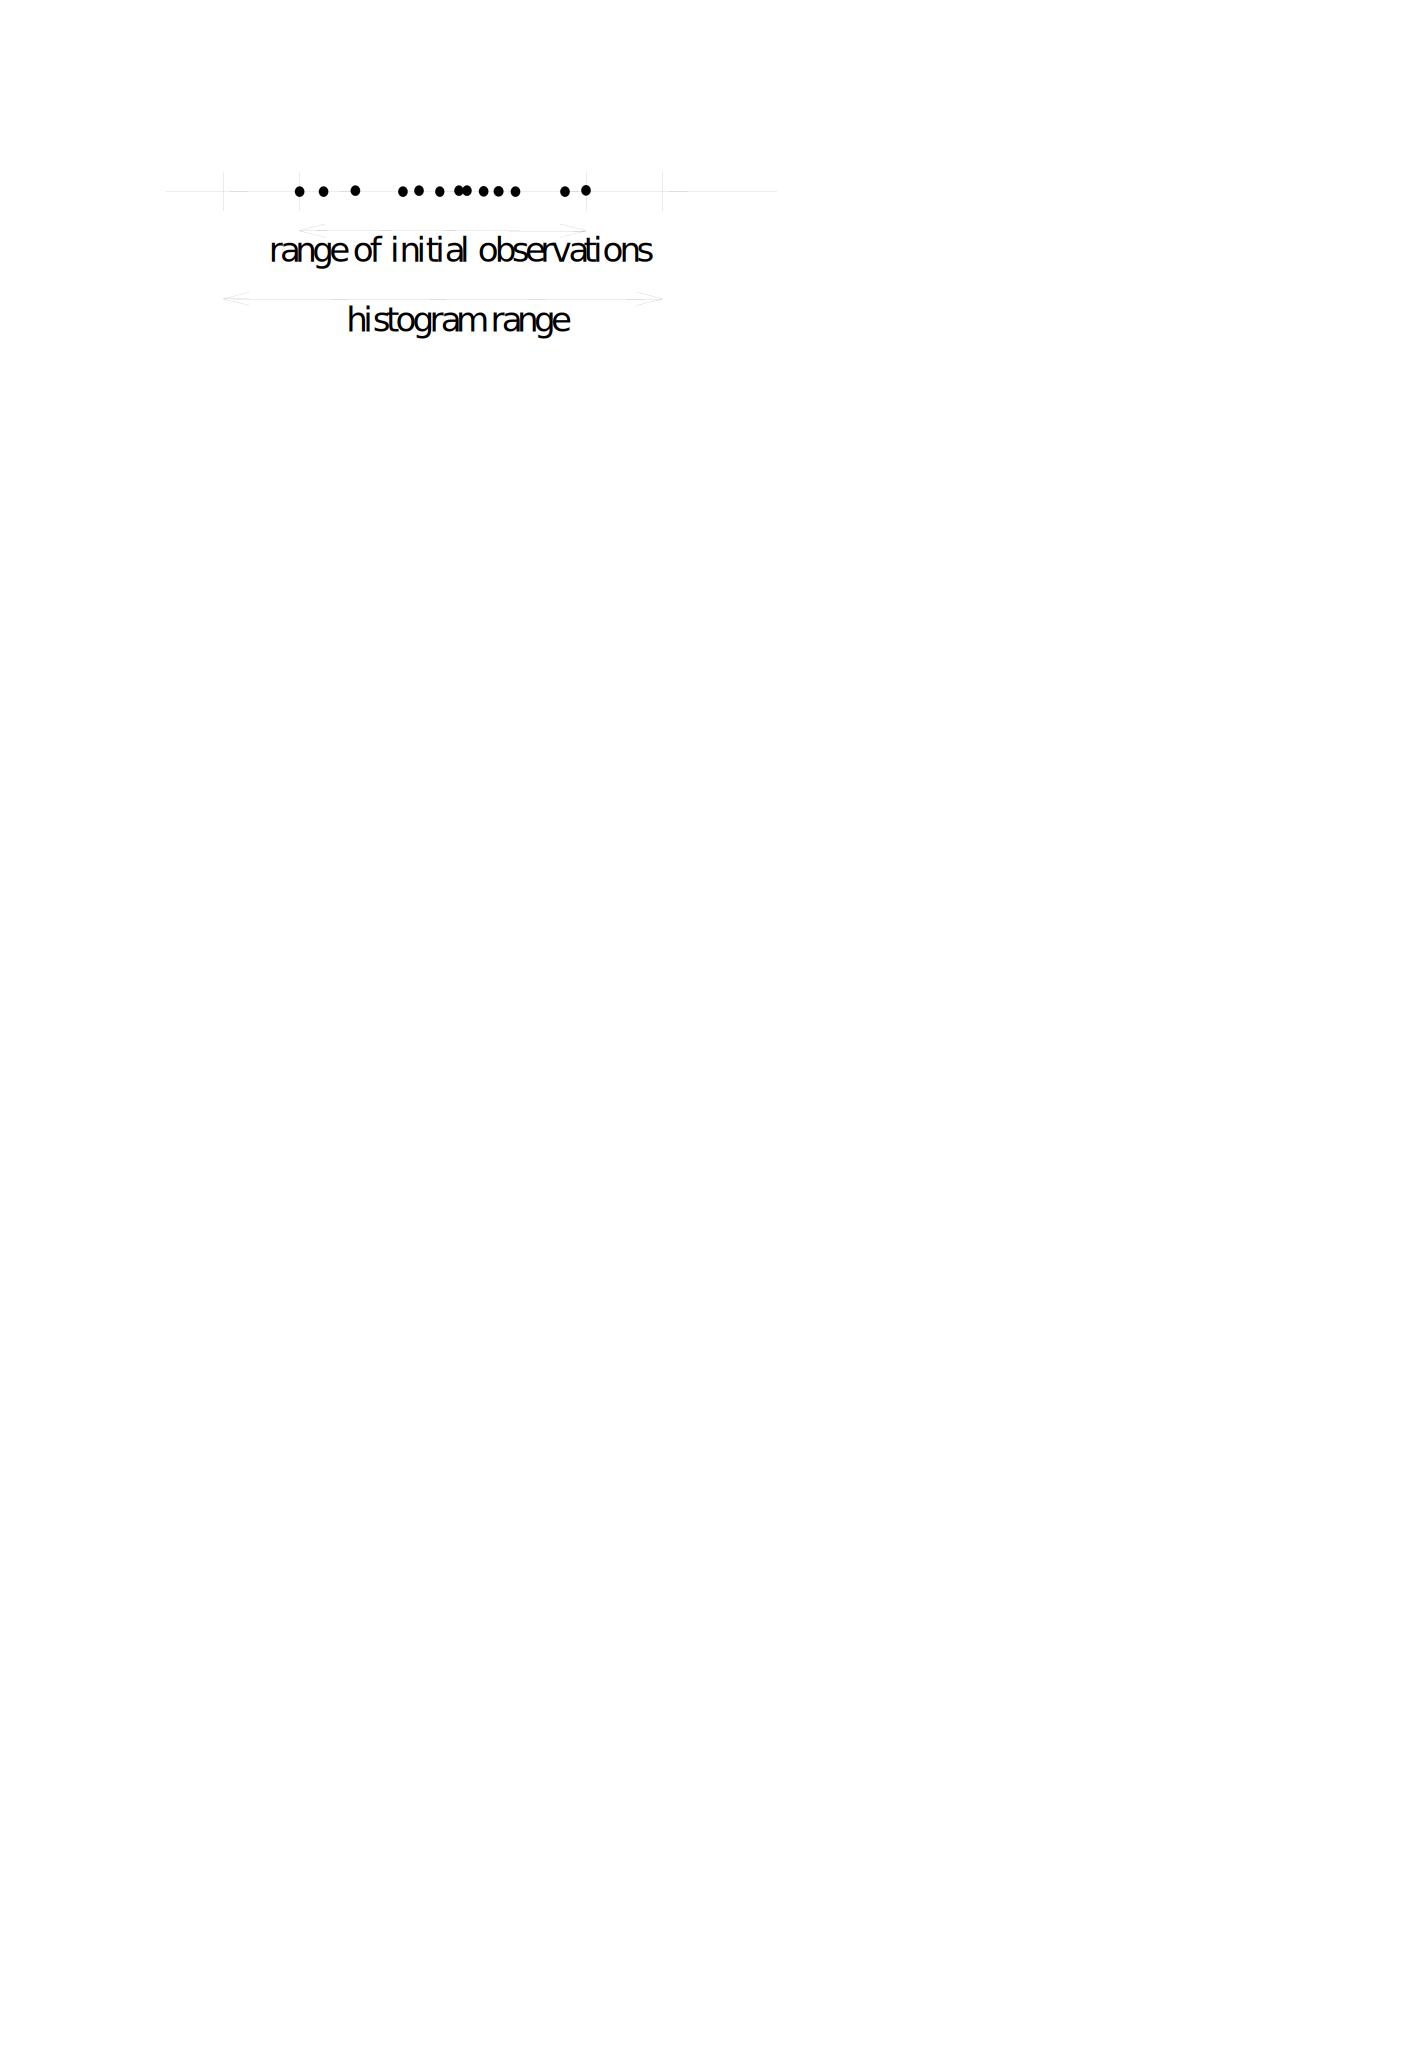
\includegraphics[width=3.215in, height=0.930in]{figures/usmanFig12}
    \caption{Setting up a histogram's range}
  \end{center}
\end{figure}

After the cells have been set up, collecting can go on.

The \fname{transformed()} function returns \textit{true} when the cells have
already been set up. You can force range estimation and setting
up the cells by calling the \fname{transform()} function.

The observations that fall outside the histogram range will be counted
as underflows and overflows. The number of underflows and overflows
are returned by the \fname{underflowCell()} and \fname{overflowCell()}
member functions.

\begin{figure}[htbp]
\begin{center}
  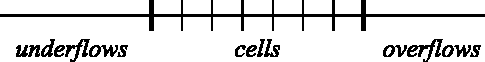
\includegraphics[width=3.310in, height=0.467in]{figures/usmanFig13}
  \caption{Histogram structure after setting up the cells}
\end{center}
\end{figure}

You create a $P^{2}$ object by specifying the number of cells:

\begin{verbatim}
cPSquare psquare("interarrival-times", 20);
\end{verbatim}

Afterwards, a \cclass{cPSquare} can be used with the same member functions
as a histogram.


\subsubsection{Getting histogram data}


There are three member functions to explicitly return cell boundaries
and the number of observations is each cell. \fname{cells()} returns
the number of cells, \fname[basepoint()]{basepoint(int k)} returns the
\textit{k}th base point, \fname[cell()]{cell(int k)} returns the
number of observations in cell \textit{k}, and
\fname[cellPDF()]{cellPDF(int k)} returns the PDF value in the cell
(i.e. between \fname[basepoint()]{basepoint(k)} and
\fname[basepoint()]{basepoint(k+1)}).  These functions work for all
histogram types, plus \cclass{cPSquare} and \cclass{cKSplit}.

\begin{figure}[htbp]
  \begin{center}
    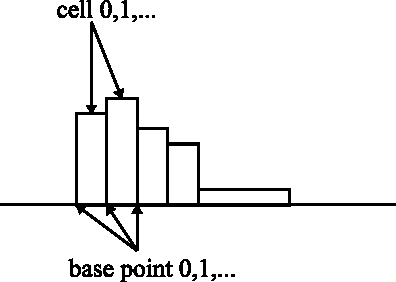
\includegraphics[width=2.615in, height=2.001in]{figures/usmanFig14}
    \caption{base points and cells}
  \end{center}
\end{figure}

An example:

\begin{verbatim}
long n = histogram.samples();
for (int i=0; i<histogram.cells(); i++)
{
  double cellWidth = histogram.basepoint(i+1)-histogram.basepoint(i);
  int count = histogram.cell(i);
  double pdf = histogram.cellPDF(i);
  //...
}
\end{verbatim}


The \fname[pdf()]{pdf(x)} and \fname[cdf()]{cdf(x)} member functions
return the value of the probability density function and the cumulated
density function at a given \textit{x}, respectively.


\subsubsection{Random number generation from distributions}


The \fname{random()} member function generates random
numbers\index{random!numbers} from the distribution stored by the
object:

\begin{verbatim}
double rnd = histogram.random();
\end{verbatim}


\cclass{cStdDev} assumes normal distribution.

You can also wrap the distribution object in a \cclass{cPar}:

\begin{verbatim}
cPar rnd_par("rnd_par");
rnd_par.setDoubleValue(&histogram);
\end{verbatim}


The \cclass{cPar} object stores the pointer to the histogram (or $P^{2}$ object),
and whenever it is asked for the value, calls the histogram object's \fname{random()}
function:

\begin{verbatim}
double rnd = (double)rnd_par; // random number from the cPSquare
\end{verbatim}

\subsubsection{Storing/loading distributions}


The statistic classes have \fname{loadFromFile()} member functions
that read the histogram data from a text file. If you need a custom
distribution\index{distribution!custom} that cannot be written (or it
is inefficient) as a C function, you can describe it in histogram form
stored in a text file, and use a histogram object with
\fname{loadFromFile()}.

You can also use \fname{saveToFile()}that writes out the distribution
collected by the histogram object:

\begin{verbatim}
FILE *f = fopen("histogram.dat","w");
histogram.saveToFile( f ); // save the distribution
fclose( f );

FILE *f2 = fopen("histogram.dat","r");}
cDoubleHistogram hist2("Hist-from-file");
hist2.loadFromFile( f2 ); // load stored distribution
fclose( f2 );
\end{verbatim}


\subsubsection{Histogram with custom cells}


The \cclass{cVarHistogram} class can be used to create
histograms with arbitrary (non-equidistant) cells.
It can operate in two modes:

\begin{itemize}
  \item \textit{manual}, where you specify cell boundaries explicitly
     before starting collecting
  \item \textit{automatic}, where \fname{transform()} will set up the cells
     after collecting a certain number of initial observations. The cells
     will be set up so that as far as possible, an equal number of observations
     fall into each cell (equi-probable cells).
\end{itemize}

Modes are selected with a \textit{transform-type} parameter:
\begin{itemize}
  \item{\ttt{HIST\_TR\_NO\_TRANSFORM}: no transformation; uses bin boundaries
    previously defined by \fname{addBinBound()}}
  \item{\ttt{HIST\_TR\_AUTO\_EPC\_DBL}: automatically creates equiprobable cells}
  \item{\ttt{HIST\_TR\_AUTO\_EPC\_INT}: like the above, but for integers}
\end{itemize}

Creating an object:

\begin{verbatim}
cVarHistogram(const char *s=NULL,
              int numcells=11,
              int transformtype=HIST_TR_AUTO_EPC_DBL);
\end{verbatim}

Manually adding a cell boundary:

\begin{verbatim}
void addBinBound(double x);
\end{verbatim}

Rangemin and rangemax is chosen after collecting the
\texttt{num\_firstvals} initial observations. One cannot add cell
boundaries when the histogram has already been transformed.





\subsection{The k-split algorithm}

\subsubsection{Purpose}


The \textit{k}-split algorithm is an on-line distribution
estimation\index{distribution!online estimation} method.  It was
designed for on-line result collection in simulation programs.  The
method was proposed by Varga and Fakhamzadeh in 1997. The primary
advantage of \textit{k}-split is that without having to store the
observations, it gives a good estimate without requiring a-priori
information about the distribution, including the sample size. The
\textit{k}-split algorithm can be extended to multi-dimensional
distributions\index{distribution!multi-dimensional}, but here we deal
with the one-dimensional version only.


\subsubsection{The algorithm}


The \textit{k-split} algorithm is an adaptive histogram-type estimate which
maintains a good partitioning by doing cell splits. We start out with
a histogram range $[x_{lo}, x_{hi})$ with $k$ equal-sized histogram
cells with observation counts $n_1,n_2, \cdots n_k$.  Each collected
observation increments the corresponding observation count. When an
observation count $n_i$ reaches a \textit{split threshold}, the cell
is split into $k$ smaller, equal-sized cells with observation counts
$n_{i,1}, n_{i,2}, \cdots n_{i,k}$ initialized to zero. The $n_i$
observation count is remembered and is called the \textit{mother
  observation count} to the newly created cells. Further observations
may cause cells to be split further (e.g. $n_{i,1,1},...n_{i,1,k}$
etc.), thus creating a $k$-order tree of observation counts where
leaves contain live counters that are actually incremented by new
observations, and intermediate nodes contain mother observation counts
for their children. If an observation falls outside the histogram
range, the range is extended in a natural manner by inserting new
level(s) at the top of the tree. The fundamental parameter to the
algorithm is the split factor $k$. Low values of $k$, $k=2$ and $k=3$
are to be considered. In this paper we examine only the $k=2$ case.

\begin{figure}[htbp]
  \begin{center}
    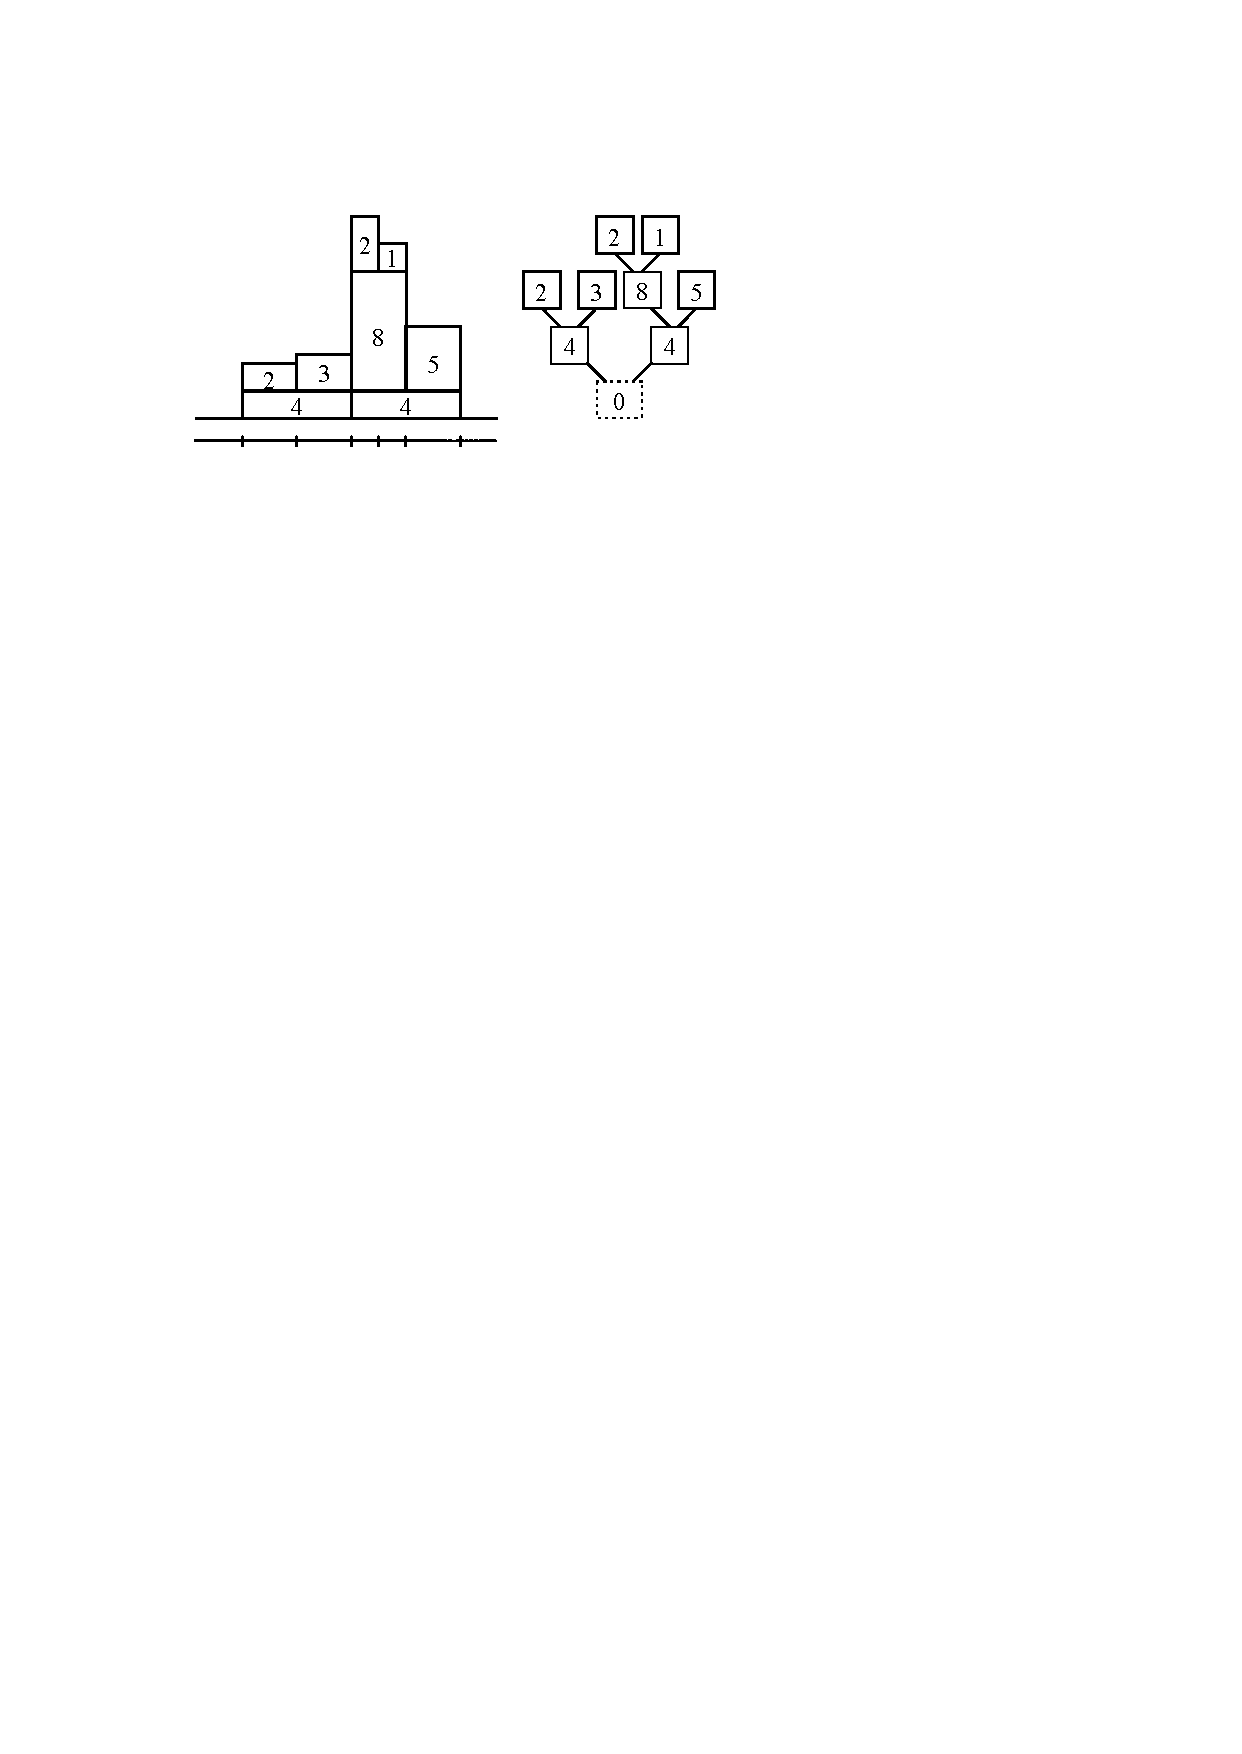
\includegraphics[width=3.442in, height=1.518in]{figures/usmanFig15}
    \caption{Illustration of the k-split algorithm, $k=2$. The
      numbers in boxes represent the observation count values}
  \end{center}
\end{figure}


For density estimation, the total number of observations that
fell into each cell of the partition has to be determined. For
this purpose, mother observations in each internal node of the
tree must be distributed among its child cells and propagated
up to the leaves.


Let $n_{...,i}$ be the (mother) observation count for a cell,
$s_{...,i}$ be the total observation count in a cell $n_{...,i}$ plus
the observation counts in all its sub-, sub-sub-, etc. cells), and
$m_{...,i}$ the mother observations propagated to the cell. We are
interested in the $\tilde{n}_{...,i} = n_{...,i} + m_{...,i}$
estimated amount of observations in the tree nodes, especially in the
leaves. In other words, if we have $\tilde{n}_{...,i}$ estimated
observation amount in a cell, how to divide it to obtain $m_{...,i,1},
m_{...,i,2} \cdots m_{...,i,k}$ that can be propagated to child cells.
Naturally, $m_{...,i,1} + m_{...,i,2} + \cdots + m_{...,i,k} =
\tilde{n}_{...,i}$.


Two natural distribution methods are even
distribution\index{distribution!even} (when $m_{...,i,1} = m_{...,i,2}
= \cdots = m_{...,i,k}$) and proportional
distribution\index{distribution!proportional} (when $m_{...,i,1} :
m_{...,i,2} : \cdots : m_{...,i,k} = s_{...,i,1} : s_{...,i,2} :
\cdots : s_{...,i,k}$). Even distribution is optimal when the
$s_{...,i,j}$ values are very small, and proportional distribution is
good when the $s_{...,i,j}$ values are large compared to
$m_{...,i,j}$. In practice, a linear combination of them seems
appropriate, where $\lambda=0$ means even and $\lambda=1$ means
proportional distribution:


\begin{equation}
m_{\cdots,i,j}=(1-\lambda )\frac{\tilde{n}_{\cdots,i}}{k} + \lambda \tilde{n}_{\cdots,i} \frac{s_{...,i,j}}{s_{\cdots,i}}, {\lambda}\in[0,1]
\end{equation}

\begin{figure}[htbp]
  \begin{center}
    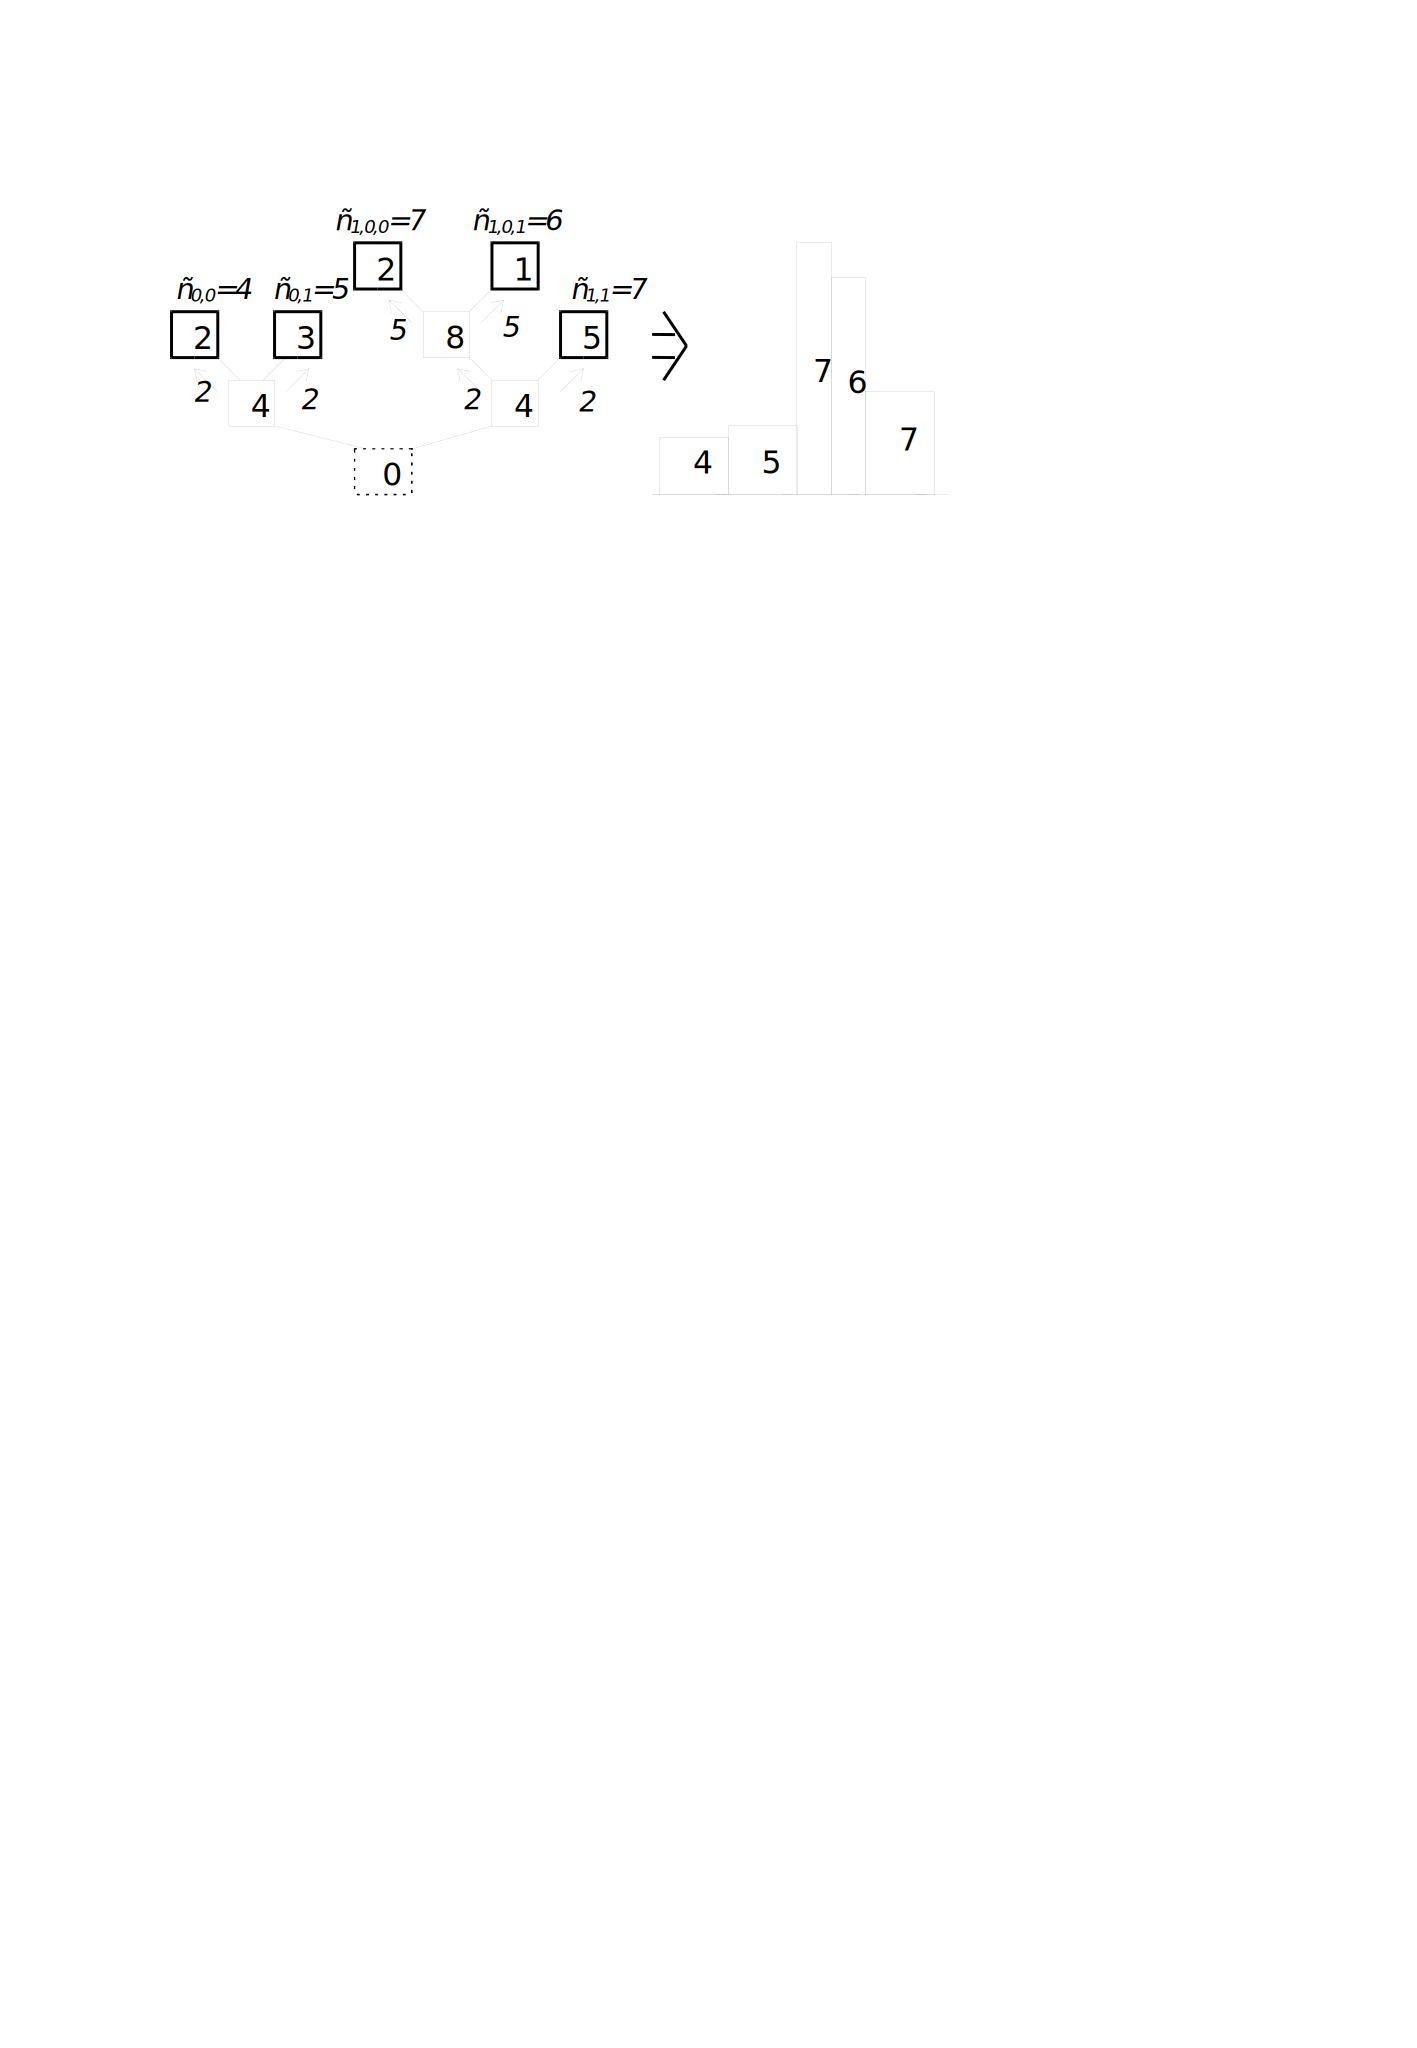
\includegraphics[width=4.147in, height=1.567in]{figures/usmanFig16}
    \caption{Density estimation from the k-split cell tree. We
      assume $\lambda=0$, i.e. we distribute mother observations
      evenly.}
  \end{center}
\end{figure}

Note that while $n_{...,i}$ are integers, $m_{...,i}$ and thus
$\tilde{n}_{...,i}$ are typically real numbers. The histogram estimate
calculated from \textit{k}-split is not exact, because the frequency
counts calculated in the above manner contain a degree of estimation
themselves. This introduces a certain \textit{cell division error};
the $\lambda$ parameter should be selected so that it minimizes that
error. It has been shown that the cell division error can
be reduced to a more-than-acceptable small value.\\
Strictly speaking, the \textit{k}-split algorithm is semi-online,
because its needs some observations to set up the initial histogram
range.  However, because of the range extension and cell split
capabilities, the algorithm is not very sensitive to the choice of the
initial range, so very few observations are enough for range
estimation (say $N_{pre}=10$). Thus we can regard \textit{k}-split as
an on-line method.

\textit{K}-split can also be used in semi-online mode, when the
algorithm is only used to create an optimal partition from a larger
number of $N_{pre}$ observations. When the partition has been created,
the observation counts are cleared and the $N_{pre}$ observations are
fed into \textit{k}-split once again. This way all mother (non-leaf)
observation counts will be zero and the cell division error is
eliminated. It has been shown that the partition created by
\textit{k}-split can be better than both the equi-distant and the
equal-frequency partition.


{\opp} contains an experimental implementation of the \textit{k}-split
algorithm, the \cclass{cKSplit} class. Research on \textit{k}-split is
still under way.


\subsubsection{The cKSplit class}

The \cclass{cKSplit} class is an implementation of the \textit{k-split} method.
Member functions:

%
% TBD comments
%

\begin{verbatim}
void setCritFunc(KSplitCritFunc _critfunc, double *_critdata);
void setDivFunc(KSplitDivFunc \_divfunc, double *\_divdata);
void rangeExtension( bool enabled );
\end{verbatim}


\begin{verbatim}
int treeDepth();
int treeDepth(sGrid& grid);
\end{verbatim}

\begin{verbatim}
double realCellValue(sGrid& grid, int cell);
void printGrids();
\end{verbatim}

\begin{verbatim}
sGrid& grid(int k);
sGrid& rootGrid();
\end{verbatim}

\begin{verbatim}
struct sGrid
{
  int parent;   // index of parent grid
  int reldepth; // depth = (reldepth - rootgrid's reldepth)
  long total;   // sum of cells & all subgrids (includes `mother')
  int mother;   // observations `inherited' from mother cell
  int cells[K]; // cell values
};
\end{verbatim}



\subsection{Transient detection and result accuracy}

In many simulations, only the steady state performance (i.e.
the performance after the system has reached a stable state)
is of interest. The initial part of the simulation is called
the transient period. After the model has entered steady state,
simulation must proceed until enough statistical data have been
collected to compute result with the required accuracy.


Detection of the end of the transient period and a certain result
accuracy is supported by {\opp}. The user can attach transient
detection\index{transient detection} and result accuracy\index{result
  accuracy} objects to a result object (\cclass{cStatistic}'s
descendants). The transient detection and result accuracy objects will
do the specific algorithms on the data fed into the result object and
tell if the transient period is over or the result accuracy has been
reached.

The base classes for classes implementing specific transient
detection and result accuracy detection algorithms are:
\begin{itemize}
\item{\cclass{cTransientDetection}: base class for transient detection}
\item{\cclass{cAccuracyDetection}: base class for result accuracy detection}
\end{itemize}


\subsubsection{Basic usage}

%
% TBD comments
%

Attaching detection objects to a \cclass{cStatistic} and getting pointers
to the attached objects:

\begin{verbatim}
addTransientDetection(cTransientDetection *object);
addAccuracyDetection(cAccuracyDetection *object);
cTransientDetection *transientDetectionObject();
cAccuracyDetection *accuracyDetectionObject();
\end{verbatim}


Detecting the end of the period:
\begin{itemize}
\item{polling the \fname{detect()} function of the object}
\item{installing a post-detect function}
\end{itemize}


\subsubsection{Transient detection}


Currently one transient detection\index{transient detection} algorithm
is implemented, i.e.  there's one class derived from
\cclass{cTransientDetection}. The \cclass{cTDExpandingWindows} class
uses the sliding window approach with two windows, and checks the
difference of the two averages to see if the transient period is over.

\begin{verbatim}
void setParameters(int reps=3,
                   int minw=4,
                   double wind=1.3,
                   double acc=0.3);
\end{verbatim}

\subsubsection{Accuracy detection}


Currently one accuracy detection\index{accuracy detection} algorithm
is implemented, i.e.  there's one class derived from
\cclass{cAccuracyDetection}. The algorithm implemented in the
\cclass{cADByStddev} class is: divide the standard deviation by the
square of the number of values and check if this is small enough.

\begin{verbatim}
void setParameters(double acc=0.1,
                   int reps=3);
\end{verbatim}




\section{Recording simulation results}

\subsection{Output vectors: cOutVector}
\label{sec:ch-sim-lib:cOutVector}

Objects of type \cclass{cOutVector} are responsible for writing time series
data (referred to as \textit{output vectors}) to a file. The \fname{record()}
member is used to output a value (or a value pair) with a timestamp.

It can be used like this:

\begin{verbatim}
cOutVector resp_v("response time");

while (...)
{
  double response_time;
  //...
  resp_v.record( response_time );
  //...
}
\end{verbatim}


All \cclass{cOutVector} objects write to the same, common file. The
file is textual; each \fname{record()} call generates a line in the
file. The output file can be processed using Plove, but otherwise its
simple format allows it to be easily processed with \fprog{sed},
\fprog{awk}, \fprog{grep} and the like, and it can be imported by
spreadsheet programs.  The file format is described later in this
manual (in the section about simulation execution).

You can disable the output vector\index{output!vector} or specify a
simulation time interval for recording either from the ini file or
directly from program code:

\begin{verbatim}
cOutVector v("v");
simtime_t t =...;

v.enable();
v.disable();
v.setStartTime( t );
v.setStopTime( t+100.0 );
\end{verbatim}


If the output vector object is disabled or the simulation time is
outside the specified interval, \fname{record()} doesn't write
anything to the output file. However, if you have a Tkenv inspector
window open for the output vector object\index{output!vector object},
the values will be displayed there, regardless of the state of the
output vector object.





\subsection{Output scalars}

While output vectors are to record time series data and thus they
typically record a large volume of data during a simulation run,
output scalars\index{output!scalars} are supposed to record a single
value per simulation run. You can use outputs scalars
\begin{itemize}
\item{to record summary data at the end of the simulation run}
\item{to do several runs with different parameter settings/random seed
    and determine the dependence of some measures on the parameter
    settings. For example, multiple runs and output scalars are the
    way to produce \textit{Throughput vs. Offered Load} plots.}
\end{itemize}

Output scalars are recorded with the \fname{recordScalar()} member
function.  It is overloaded, you can use it to write doubles and
strings (const char *):

\begin{verbatim}
double avg_throughput = total_bits / simTime();
recordScalar("Average throughput", avg_throughput);
\end{verbatim}

You can record whole statistics objects by calling \fname{recordStats()}:

\begin{verbatim}
cStdDev *eedstats = new cStdDev;
...
recordStats("End-to-end Statistics", eedstats);
\end{verbatim}

Calls to \fname{recordScalar()} and \fname{recordStats()} are usually
placed in the redefined \fname{finish()} member function of a
simple module.

The above calls write into the (textual) output scalar file.  The
output scalar file is preserved across simulation runs (unlike the
output vector file is, scalar files are not deleted at the beginning
of each run). Data are always appended at the end of the file, and
output from different simulation runs are separated by special lines.




\section{Tracing and debugging aids}

\subsection{Displaying information about module activity}

You can have simple modules print textual output for
debugging\index{debugging} purposes.

The global object called \ttt{ev} represents the user interface of the
simulation program. You can send data to \ttt{ev}\index{ev} using the
C++-style I/O operator (\ttt{<}\ttt{<}).

\begin{verbatim}
ev << "started\n";
ev << "about to send message #" <<  i << endl;
ev << "queue full, discarding packet\n";
\end{verbatim}

The more traditional-looking but functionally equivalent
\fname{ev.printf()} form also exists.

\begin{verbatim}
ev.printf("%d packets dropped out of %d\n", drops, total);
\end{verbatim}

The exact way messages are displayed to the user depends on the user
interface. In the command-line user interface (Cmdenv\index{Cmdenv}),
it is simply dumped to the standard output. (This output can also be
disabled from the ini file so that it doesn't slow down simulation
when it is not needed.) In windowing user interfaces
(Tkenv\index{Tkenv}), each simple module can have
a separate text output window.

The above means that you should \textit{not} use \fname{printf()},
\fname{cout} \fname{<<} and the like because with Tkenv, their output
would appear in the terminal window behind the graphical window of the
simulation application.


\subsection{Watches}

You may want some of your int, long, double, char, etc. variables to
be inspect-able in Tkenv and to be output into the snapshot
file\index{snapshot file}. In this case, you can create
\cclass{cWatch} objects for them with the \fmac{WATCH()} macro:

\begin{verbatim}
int i; WATCH(i);
char c; WATCH(c);
\end{verbatim}

When you open an inspector for the simple module in Tkenv and click
the Objects/Watches tab in it, you'll see your WATCHed variables
and their values there. Tkenv also lets you change the value of a
WATCHed variable.

The \fmac{WATCH()} macro expands to a dynamically created \cclass{cWatch}
object.  The object remembers the address and type of your variable.
The macro expands to something like:

\begin{verbatim}
new cWatch("i",i);
\end{verbatim}


You can also make a \texttt{WATCH} for pointers of type \ttt{char*} or
\cclass[cObject]{cObject*}, but this may cause a segmentation fault if
the pointer does not point to a valid location when Tkenv or
\fname{snapshot()} wants to use it.

You can also set watches for variables that are members of the
module class\index{module!watches} or for structure fields:

\begin{verbatim}
WATCH( lapbconfig.timeout );
\end{verbatim}


\subsubsection{Placement of WATCHes}


Be careful not to execute a \fmac{WATCH()} statement more than once,
as each call would create a new \cclass{cWatch} object! If you use
\fname{activity()}, the best place for WATCHes is the top of the
\fname{activity()} function.  If you use \fname{handleMessage()},
place the \fname{WATCH()} statement into \fname{initialize()}.
\fname{WATCH()} creates a dynamic \cclass{cWatch} object, and we do
not want to create a new object each time \fname{handleMessage()} is
called.



\subsection{Snapshots}
\label{sec:ch-sim-lib:snapshots}

The \fname{snapshot()} function outputs textual information about all
or selected objects of the simulation (including the objects created
in module functions by the user) into the snapshot file\index{snapshot file}.

\begin{verbatim}
bool snapshot(cObject *obj = &simulation, const char *label = NULL);
\end{verbatim}


The function can be called from module functions, like this:

\begin{verbatim}
snapshot();     // dump the whole network
snapshot(this); // dump this simple module and all its objects
snapshot(&simulation.msgQueue); // dump future events
\end{verbatim}

This will append snapshot information to the end of the snapshot file.
(The snapshot file name has an extension of \ttt{.sna}, default is
\ttt{omnetpp.sna}\index{omnetpp.sna}. Actual file name can be set in the
config file.)


The snapshot file output is detailed enough to be used for debugging
the simulation: by regularly calling \fname{snapshot()}, one can trace
how the values of variables, objects changed over the simulation.
The arguments: label is a string that will appear in the output
file; obj is the object whose inside is of interest. By default,
the whole simulation (all modules etc) will be written out.

If you run the simulation with Tkenv, you can also create a snapshot
from the menu.


An example of a snapshot file:

\begin{Verbatim}[commandchars=\\\{\}]
================================================
|| SNAPSHOT ||
================================================
| Of object:    `simulation'
| Label:        `three-station token ring'
| Sim. time:    0.0576872457 ( 57ms)
| Network:      `token'
| Run no.       1
| Started at:   Mar 13, 1997, 14:23:38
| Time:         Mar 13, 1997, 14:27:10
| Elapsed:      5 sec
| Initiated by: operator
================================================


(cSimulation) `simulation' begin
  Modules in the network:
    `token' #1 (TokenRing)
      `comp[0]' #2 (Computer)
        `mac' #3 (TokenRingMAC)
        `gen' #4 (Generator)
        `sink' #5 (Sink)
      `comp[1]' #6 (Computer)
        `mac' #7 (TokenRingMAC)
        `gen' #8 (Generator)
        `sink' #9 (Sink)
      `comp[2]' #10 (Computer)
        `mac' #11 (TokenRingMAC)
        `gen' #12 (Generator)
        `sink' #13 (Sink)
end

(cCompoundModule) `token' begin
  #1 params     (cArray) (n=6)
  #1 gates      (cArray) (empty)
  comp[0]          (cCompoundModule,#2)
  comp[1]          (cCompoundModule,#6)
  comp[2]          (cCompoundModule,#10)
end

(cArray) `token.parameters' begin
  num_stations (cModulePar) 3 (L)
  num_messages (cModulePar) 10000 (L)
  ia_time      (cModulePar) truncnormal(0.005,0.003) (F)
  THT          (cModulePar) 0.01 (D)
  data_rate    (cModulePar) 4000000 (L)
  cable_delay  (cModulePar) 1e-06 (D)
end

(cModulePar) `token.num_stations' begin
  Type: L
  Value: 3
end

\textit{[...token.num_messages omitted...]}

(cModulePar) `token.ia_time' begin
  Type:  F
  Value: truncnormal(0.005,0.003)
end

\textit{[...rest of parameters \& gates stuff deleted from here...]}

(cCompoundModule) `token.comp[0]' begin
  parameters    (cArray) (empty)
  gates         (cArray) (n=2)
  mac           (TokenRingMAC,#3)
  gen           (Generator,#4)
  sink          (Sink,#5)
end

(cArray) `token.comp[0].parameters' begin
end

(cArray) `token.comp[0].gates' begin
  in            (cGate)  <-- comp[2].out
  out           (cGate)  --> D --> comp[1].in
end

(cGate) `token.comp[0].in' begin
  type:  input
  inside connection:  token.comp[0].mac.phy_in
  outside connection: token.comp[2].out
  delay: -
  error: -
  data rate: -
end

(cGate) `token.comp[0].out' begin
  type: output
  inside connection: token.comp[0].mac.phy_out
  outside connection: token.comp[1].in
  delay: (cPar) 1e-06 (D)
  error: -
  data rate: -
end

(TokenRingMAC) `token.comp[0].mac' begin
  parameters    (cArray) (n=2)
  gates         (cArray) (n=4)
  local-objects (cHead)
  class-data-members (cHead)
end

\textit{[...comp[0].mac parameters stuff deleted from here...]}

(cArray) `token.comp[0].mac.gates' begin
  phy_in        (cGate)  <-- <parent>.in
  from_gen      (cGate)  <-- gen.out
  phy_out       (cGate)  --> <parent>.out
  to_sink       (cGate)  --> sink.in
end

\textit{[...detailed gate list deleted from here...]}

(cHead) `token.comp[0].mac.local-objects' begin
  sendqueue-length (cOutVector) (single)
  send-queue   (cQueue) (n=11)
end

(cOutVector) `token.comp[0].mac.local-objects.sendqueue-length' begin
end

(cQueue) `token.comp[0].mac.local-objects.send-queue' begin
  0-->1         (cMessage) Tarr=0.0158105774 ( 15ms) Src=#4 Dest=#3
  0-->2         (cMessage) Tarr=0.0163553310 ( 16ms) Src=#4 Dest=#3
  0-->1         (cMessage) Tarr=0.0205628236 ( 20ms) Src=#4 Dest=#3
  0-->2         (cMessage) Tarr=0.0242203591 ( 24ms) Src=#4 Dest=#3
  0-->2         (cMessage) Tarr=0.0300994268 ( 30ms) Src=#4 Dest=#3
  0-->1         (cMessage) Tarr=0.0364005251 ( 36ms) Src=#4 Dest=#3
  0-->1         (cMessage) Tarr=0.0370745702 ( 37ms) Src=#4 Dest=#3
  0-->2         (cMessage) Tarr=0.0387984129 ( 38ms) Src=#4 Dest=#3
  0-->1         (cMessage) Tarr=0.0457462493 ( 45ms) Src=#4 Dest=#3
  0-->2         (cMessage) Tarr=0.0487308918 ( 48ms) Src=#4 Dest=#3
  0-->2         (cMessage) Tarr=0.0514466766 ( 51ms) Src=#4 Dest=#3
end

(cMessage) `token.comp[0].mac.local-objects.send-queue.0-->1' begin
  #4 --> #3
  sent:         0.0158105774 ( 15ms)
  arrived:      0.0158105774 ( 15ms)
  length:       33536
  kind:         0
  priority:     0
  error:        FALSE
  time stamp:   0.0000000 ( 0.00s)
  parameter list:
    dest        (cPar) 1 (L)
    source      (cPar) 0 (L)
    gentime     (cPar) 0.0158106 (D)
end

(cArray) `token.comp[0].mac.local-objects.send-queue.0-->1.par-vector' begin
  dest          (cPar) 1 (L)
  source        (cPar) 0 (L)
  gentime       (cPar) 0.0158106 (D)
end

\textit{[...message parameters and the other messages' stuff deleted...]}

(cHead) `token.comp[0].mac.class-data-members' begin
end

\textit{[...comp[0].gen and comp[0].sink stuff deleted from here...]}
\textit{[...whole comp[1] and comp[2] stuff deleted from here...]}

(cMessageHeap) `simulation.message-queue' begin
  1-->0         (cMessage) Tarr=0.0576872457 ( 57ms) Src=#8 Dest=#7
                (cMessage) Tarr=0.0577201630 ( 57ms) Mod=#8 (selfmsg)
                (cMessage) Tarr=0.0585677054 ( 58ms) Mod=#4 (selfmsg)
                (cMessage) Tarr=0.0594939072 ( 59ms) Mod=#12 (selfmsg)
                (cMessage) Tarr=0.0601010000 ( 60ms) Mod=#7 (selfmsg)
  1-->2         (cMessage) Tarr=0.0601020000 ( 60ms) Src=#11 Dest=#13
end

\textit{[...detailed list of message queue contents deleted from here...]}
\end{Verbatim}





\subsection{Breakpoints}

\textbf{With activity() only!} In those user interfaces which support
debugging, breakpoints stop execution and the state of the simulation
can be examined.

You can set a breakpoint\index{breakpoint} inserting a
\fname{breakpoint()} call into the source:

\begin{verbatim}
for(;;)
{
  cMessage *msg = receive();
  breakpoint("before-processing");
  breakpoint("before-send");
  send( reply_msg, "out" );
  //..
}
\end{verbatim}


In user interfaces that do not support debugging, \fname{breakpoint()}
calls are simply ignored.





\subsection{Disabling warnings}

Some container classes and functions suspend the simulation and issue
warning messages in potentially bogus/dangerous situations, for
example when an object is not found and NULL pointer/reference is
about to be returned. Very often this is useful, but sometimes it is
more trouble. You can turn warnings on/off from the ini file
(warnings=yes/no)\index{ini file!warnings}.


It is a good practice to leave warnings\index{warnings} enabled, and
temporarily disable warnings in places where {\opp} would normally
issue warnings but you know the code is correct. This is done in the
following way:

\begin{verbatim}
bool w = simulation.warnings();
simulation.setWarnings( false );
...
... // critical code
...
simulation.setWarnings( w );
\end{verbatim}





\subsection{Getting coroutine stack usage}

It is important to choose the correct stack size for
modules\index{module!stack size}\index{stack!size}.  If the stack is
too large, it unnecessarily consumes memory; if it is too small, stack
violation occurs.

From the Feb99 release, {\opp} contains a mechanism that detects stack
overflows\index{stack!overflow}. It checks the intactness of a
predefined byte pattern (\texttt{0xdeadbeef}) at the stack boundary,
and reports ``stack violation''\index{stack!violation} if it was
overwritten. The mechanism usually works fine, but occasionally it can
be fooled by large -- and not fully used -- local variables (e.g. char
buffer[256]): if the byte pattern happens to fall in the middle of
such a local variable, it may be preserved intact and {\opp} does not
detect the stack violation.

To be able to make a good guess about stack size, you can use
the \fname{stackUsage()} call which tells you how much stack the module
actually uses. It is most conveniently called from \fname{finish()}:

\begin{verbatim}
void FooModule::finish()
{
  ev << stackUsage() <<  "bytes of stack used\n";
}
\end{verbatim}


The value includes the extra stack added by the user interface library
(see \textit{extraStackforEnvir}\index{extraStackforEnvir} in
envir/omnetapp.h), which is currently 8K for Cmdenv and at least 16K
for Tkenv.
  \footnote{The actual value is dependent on the operating
  system, e.g. SUN Solaris needs more space.}

\fname{stackUsage()}also works by checking the existence of predefined
byte patterns in the stack area, so it is also subject to the above
effect with local variables.


\section{Changing the network graphics at run-time}

\subsection{Setting display strings}

Sometimes it is useful to change the appearance or position of
some components in the network graphics, such as the color of the
modules\index{module!color}, color/width of connection arrows,
position of a submodule, etc.

The appearance of nodes and connections is determined by the display
strings\index{display strings}. Display strings (e.g. \ttt{"p=100,10;i=pc"})
are initially taken from the NED description.
You can change the display string of a module or connection arrow
at run-time by calling methods named \fname{setDisplayString()}.
The \cclass{cDisplayStringParser} class (discussed in the following sections)
might be useful for manipulating the display string.

Setting the module's appearance when it is displayed as a component
within a compound module:

\begin{verbatim}
setDisplayString("p=100,100;b=60,30,rect;o=red,black,3", true);
\end{verbatim}

Setting appearance of a compound module when it's displayed as a
bounding box for its submodules:

\begin{verbatim}
parentModule()->setDisplayStringAsParent("p=100.....", true);
\end{verbatim}

The display string of a connection arrow\index{arrow display string}
is stored in its source gate, so you'll need to write something
like this:

\begin{verbatim}
gate("out")->setDisplayString("o=yellow,3");
\end{verbatim}

The \fname{setDisplayString()} methods additionally take a bool
argument called \fvar{immediate}. It specifies whether the display
string change should take effect immediately, or only after processing
the current event (the default is \textit{immediate=true}). If several
display string changes are going to be done within one event, then
\textit{immediate=false} is useful because it reduces the number of
necessary redraws. \textit{Immediate=false} also uses less stack.  But
its drawback is that a \fname{setDisplayString()} followed by a
\fname{send()} would actually be displayed in reverse order (message
animation first), because message animations are performed immediately
(actually within the \fname{send()} call).


\subsection{The cDisplayStringParser class}

The \cclass{cDisplayStringParser} utility class lets you parse and
manipulate display strings.

As far as \cclass{cDisplayStringParser} is concerned, a display string
(e.g. \ttt{"p=100,125;i=cloud"}) is a string that consist of several
\textit{tags} separated by semicolons, and each tag has a \textit{name}
and after an equal sign, zero or more \textit{arguments} separated by commas.

The class facilitates tasks such as finding out what tags a display string
has, adding new tags, adding arguments to existing tags,
removing tags or replacing arguments. The internal storage method allows
very fast operation; it will generally be faster than direct string manipulation.
The class doesn't try to interpret the display string in any way, nor does
it know the meaning of the different tags; it merely parses the string
as data elements separated by semicolons, equal signs and commas.

An example:

\begin{Verbatim}
cDisplayStringParser dispstr("a=1,2;p=alpha,,3");
dispstr.insertTag("x");
dispstr.setTagArg("x",0,"joe");
dispstr.setTagArg("x",2,"jim");
dispstr.setTagArg("p",0,"beta");
ev << dispstr.getString();  // result: "x=joe,,jim;a=1,2;p=beta,,3"
\end{Verbatim}





\section{Deriving new classes}

\subsection{cObject or not?}

If you plan to implement a completely new class (as opposed to
subclassing something already present in {\opp}), you have
to ask yourself whether you want the new class to be based
on \cclass{cObject} or not.
Note that we're \textit{not} saying you should always
subclass from \cclass{cObject}.
Both solutions have advantages and disadvantages which you
have to consider individually for each class.

\cclass{cObject} already carries (or provides framework for)
significant functionality that are either important for
your particular purpose or not. Subclassing \cclass{cObject}
generally means you have more code to write (as you \textit{have to}
redefine certain virtual functions and adopt to conventions)
and your class will be a bit more heavy-weight.
In turn, it will integrate into OMNeT++ better, for example
it will be more visible in Tkenv and can be automatically
garbage-collected (this will be discussed later). If you
need to store your objects in {\opp} objects like \cclass{cQueue},
or you'll want to store {\opp} classes in your object,
then you \textit{must} subclass from \cclass{cObject}.
  \footnote{For simplicity, in the these sections ``{\opp} object''
  should be understood as ``object of a class subclassed from
  \cclass{cObject}''}

The most significant features \cclass{cObject} has is
the name string (which has to be stored somewhere, so it has
its overhead) and ownership management (see section
\ref{sec:ch-sim-lib:ownership-management}) which
also has the advantages but also some costs.

As a general rule, small \ttt{struct}-like classes like \ttt{IPAddress},
\ttt{MACAddress}, \ttt{RoutingTableEntry}, \ttt{TCPConnectionDescriptor}, etc.
are better \textit{not} sublassed from \cclass{cObject}.
On the other hand, if you want to store your objects in {\opp} objects
like \cclass{cQueue}, or you'll want to store {\opp} classes in your object,
then you \textit{must} subclass from \cclass{cObject}.
If your class fits neither category, you'll need to
see if \cclass{cObject} brings any benefit for you, and
decide accordingly.


\subsection{cObject virtual methods}

Most classes in the simulation class library are descendants of
\cclass{cObject}. If you want to derive a new class from
\cclass{cObject} or a \cclass{cObject} descendant, you must redefine
some member functions so that objects of the new type can fully
co-operate with other parts of the simulation system. A more or less
complete list of these functions is presented here. Do not be
embarrassed at the length of the list: most functions are not
absolutely necessary to implement. For example, you do not need to
redefine \fname{forEach()} unless your class is a container class.

The following methods \textbf{must} be implemented:

\begin{itemize}
  \item{\textit{Constructor}. At least two constructors should be provided:
        one that takes the object name string as \ttt{const char *}
        (recommended by convention), and another one with no arguments
        (must be present). The two are usually implemented as a single
        method, with \ttt{NULL} as default name string.}
  \item{\textit{Copy constructor}, which must have the following signature
        for a class \ttt{X}: \ttt{X(const X\&)}. The copy constructor is used
        whenever an object is duplicated. The usual implementation of
        the copy constructor is to initialize the base class with the
        name (\fname{name()}) of the other object it receives, then call the
        assignment operator (see below).}
  \item{\textit{Destructor}. Any good-tempered class has a destructor.}
  \item{\textit{Duplication function,} \fname{cObject *dup() const}.
        It should create and return an exact duplicate of the object.
        It is usually a one-line function, implemented with the help
        of the \ttt{new} operator and the copy constructor.}
  \item{\textit{Assigment operator}, that is, \ttt{X\& operator=(const X\&)}
        for a class \ttt{X}. It should copy the contents of the other
        object into this one, except the name string. See later what to do
        if the object contains pointers to other objects.}
\end{itemize}

The following function \textbf{should} be implemented if your class contains
via pointers or as data member) other object subclassed from \cclass{cObject}.

\begin{itemize}
  \item{\textit{Iteration function,} \ttt{void forEach(ForeachFunc f)}.
        The implementation should call the function passed
        for each object it contains via pointer or
        as data member; see the API Reference on \cclass{cObject} on how to
        implement \ttt{foreach()}. \fname{foreach()} is used by Tkenv and
        \fname{snapshot()} to navigate, search or display the object tree.}
\end{itemize}

The following methods are \textbf{recommended} to implement:

\begin{itemize}
  \item{\textit{Object info,} \fname{void info(char *)}. The \ttt{info()} function
        should print a one-line info about object contents into the given
        buffer -- usually the class name, the object name, important state variables, etc.
        This is used when Tkenv displays list of objects (in the object tree
        or in listboxes). The length of the info should not exceed 500 chars.}
  \item{\textit{Detailed object info,} \fname{void writeContents(ostream\&)}.
        It should write a detailed multi-line report about the object contents
        into the stream provided. This is currently only used by \fname{snapshot()}.}
\end{itemize}

%% FIXME todo
%%
%% Necessary for parallel execution:
%%
%% \begin{itemize}
%%  \item{\fname{netPack()}, \fname{netUnpack()}: they are needed only if
%%        objects of this type will be transmitted over LPs.}
%% \end{itemize}



\subsection{Class registration}

You should also use the \fmac{Register\_Class()} macro to register the
new class. It is used by the \fname{createOne()} function.



\subsection{Details}

We'll go through the details using an example. We create a new
class \ttt{NewClass}, redefine all above mentioned \cclass{cObject}
member functions, and explain the conventions, rules and tips
associated with them.
To demonstrate as much as possible, the class will contain
an \ttt{int} data member, dynamically allocated non-\cclass{cObject} data
(an array of \cclass{double}s),
an {\opp} object as data member (a \ttt{cQueue}), and
a dynamically allocated {\opp} object (a \ttt{cMessage}).

The class declaration is the following. It contains the declarations
of all methods discussed in the previous section.

\begin{verbatim}
//
// file: newclass.h
//
#include <omnetpp.h>

class NewClass : public cObject
{
  protected:
    int data;
    double *array;
    cQueue queue;
    cMessage *msg;
    ...
  public:
    NewClass(const char *name=NULL, int d=0);
    NewClass(const NewClass& other);
    virtual ~NewClass();
    virtual cObject *dup() const;
    NewClass& operator=(const NewClass& other);

    virtual void foreach(ForeachFunc f);

    virtual void info(char *buf);
    virtual void writeContents(ostream& os);
    ...
};
\end{verbatim}

We'll discuss the implementation method by method.
Here's the top of the \ttt{.cc} file:

\begin{verbatim}
//
// file: newclass.cc
//
#include <stdio.h>
#include <string.h>
#include <iostream.h>
#include "newclass.h"

Register_Class( NewClass );


NewClass::NewClass(const char *name, int d) : cObject(name)
{
    data = d;
    array = new double[10];
    take(&queue);
    msg = NULL;
}
\end{verbatim}

The constructor (above) calls the base class constructor with
the name of the object, then initializes its own data members.
\cclass{cObject}-based data members should have their
owners explicitly set to NULL.


\begin{verbatim}
NewClass::NewClass(const NewClass& other) : cObject(name())
{
    array = new double[10];
    msg = NULL;
    take(&queue);
    operator=(other);
}
\end{verbatim}

The copy constructor relies on the assignment operator. Because
by convention the assignment operator does not copy the
name member, it is passed here to the base class constructor.
(Alternatively, we could have written \ttt{setName(other.name())}
into the function body.)

Note that pointer members have to be initialized (to \ttt{NULL} or to an
allocated object/memory) before calling the assignment operator,
to avoid crashes.

\cclass{cObject}-based data members should have their
owners explicitly set to NULL.

\begin{verbatim}
NewClass::~NewClass()
{
    delete [] array;
    if (msg->owner()==this)
        delete msg;
}
\end{verbatim}

The destructor should delete all data structures the object allocated.
\cclass{cObject}-based objects should \textit{only} be deleted if they
are owned by the object -- details will be covered in section
\ref{sec:ch-sim-lib:ownership-management}.

\begin{verbatim}
cObject *NewClass::dup() const
{
    return new NewClass(*this);
}
\end{verbatim}

The \ttt{dup()} functions is usually just one line, like the one above.

\begin{verbatim}
NewClass& NewClass::operator=(const NewClass& other)
{
    if (&other==this)
        return *this;
    cObject::operator=(other);

    data = other.data;

    for (int i=0; i<10; i++)
        array[i] = other.array[i];

    queue = other.queue;
    queue.setName(other.queue.name());

    if (msg && msg->owner()==this)
        delete msg;
    if (other.msg && other.msg->owner()==const_cast<cMessage*>(&other))
        take(msg = (cMessage *)other.msg->dup());
    else
        msg = other.msg;
    return *this;
}
\end{verbatim}

Complexity associated with copying and duplicating the object
is centralized in the assignment operator, so it is usually
the one that requires the most work from you of all methods
required by \cclass{cObject}.

If you do not want to implement object copying and duplication,
you should implement the assigment operator to call
\fname{copyNotSupported()} -- it'll throw an exception that
stops the simulation with an error message if this function
is called.

The assignment operator copies contents of the \ttt{other} object
to this one, except the name string. It should always return
\ttt{*this}.

First, we should make sure we're not trying to copy the object
to itself, because it might be disastrous. If so (that is,
\ttt{\&other==this}), we return immediately without doing anything.

The base class part is copied via invoking the assignment operator of
the base class.

New data members are copied in the normal C++ way. If the class
contains pointers, you'll most probably want to make a deep copy of
the data where they point, and not just copy the pointer values.

If the class contains pointers to {\opp} objects, you need
to take ownership into account. If the contained object is \textit{not owned}
then we assume it is a pointer to an ``external'' object, consequently
we only copy the pointer. If it is \textit{owned}, we duplicate
it and become the owner of the new object. Details of ownership
management will be covered in section \ref{sec:ch-sim-lib:ownership-management}.


\begin{verbatim}
void NewClass::forEach(ForeachFunc f)
{
    if (f(this,true))
    {
        queue->forEach(f);
        if (msg)
            msg->forEach(f);
    }
    f(this,false);
}
\end{verbatim}

The \fname{foreach()} function should be called for each {\opp}
member of the class. See the API Reference for more information
of \fname{foreach()}.

\begin{verbatim}
void NewClass::info(char *buf)
{
    cObject::info(buf);
    sprintf(buf+strlen(buf), " data=%d, array[0]=%g, %s",
            data, array[0], (msg ? "has msg" : "no msg"));
}
\end{verbatim}

Here you should produce a concise, one-line info about the object.
You should try not to exceed 40-80 characters, since the
string will be shown in tooltips and listboxes. The length
of the buffer is 500 bytes, so in any case you should not
exceed that length. You can make use of \cclass{cObject}'s
\ttt{info()} method that produces the class name and the object name.

\begin{verbatim}
void NewClass::writeContents(ostream& os)
{
    os << " data: " << data << endl;
    os << " array: "
    for (int i=0; i<10; i++)
        os << array[i] << " ";
    os << endl;
}
\end{verbatim}

\fname{writecontents()} is expected to write values of all
data members to the stream.  You do not need to include anything
about contained \cclass{cObject}-based objects, because they
will be included via \fname{foreach()}.


See the virtual functions of \cclass{cObject} in the class library reference
for more information. The sources of the Sim library (\ttt{include/},
\ttt{src/sim/}) can serve as further examples.




\section{Object ownership management}
\label{sec:ch-sim-lib:ownership-management}

{\opp} has a built-in ownership management mechanism which
is used for garbage collection, sanity checks, and as
part of the infrastructure supporting Tkenv inspectors.
It usually works transparently, but it is useful to know
what it does exactly so that it doesn't interfere
with the cleanup code and destructors you write.

If you plan to program small simple modules only, you can probably
safely skip this section. But if your simple module code
is getting more complex and you're getting memory leaks or seemingly
unexplicable segmentation faults because of double deletion of objects,
it is probably time to read the following discussion.


\subsection{Ownership tree}

Any \cclass{cObject}-based object can be both \textit{owner} of other
objects and can at the same time be \textit{owned} by another object.
For example, a message object (\fname{cMessage}) may reside
in a queue (\cclass{cQueue}) and be owned by that queue, while it
may own attached \fname{cPar} objects or another message
(added to it via \fname{encapsulate()}).

From an object you can navigate to its owner by calling the \fname{owner()}
method, defined in \cclass{cObject}. The other direction, enumerating the
objects owned can be done via \fname{foreach()} that loops through all
contained objects and checking the owner of each object.


\subsection{Purpose}

The purpose of maintaining the ownership tree is threefold:

\begin{itemize}
    \item{to provide a certain degree of garbage collection (that is,
    automatic deletion of objects that are no longer needed)}

    \item{to prevent a certain types of programming errors, namely,
    those associated with wrong ownership handling.}

    \item{it provides some ``reflection'' (in the Java sense), which
    enables Tkenv to display which objects are present (and where)
    in the simulation, to find ``lost'' (leaked) objects, etc.}
\end{itemize}

Some examples of programming errors that can be caught
by the ownership facility:

\begin{itemize}
    \item{attempts to send a message while it's still in a queue,
    encapsulated in another message, etc.}

    \item{attempts to send/schedule a message while it's still owned
    by the simulation kernel (i.e. scheduled as a future event)}

    \item{attempts to send the very same message object to multiple
    destinations at the same time (ie. to all connected modules)}
\end{itemize}

The above errors are easy to make in the code, and if not
detected automatically, they could cause random crashes
which are usually very difficult to track down.

Of course, some errors of the same kind still cannot be detected
automatically, like calling member functions of a message object
which has been sent to (and so currently kept by) another module.


\subsection{Objects are deleted by their owners}

The concept of \fname{ownership} is that \textit{the owner has the
exclusive right and duty to delete the objects it owns}.

As an example, this means if you delete a message, its encapsulated
message (see \fname{encapsulate()} method) and attached
\fname{cPar} objects are also deleted. If you delete a queue,
all messages it contains and also owns will also be deleted.
  \footnote{Note that it's not necessary for a container object like
  a queue to actually own all inserted objects. This behavior
  can be controlled via the \textit{takeownership} flag,
  as explained later.}

If you create a new class, you should implement it so that
it deletes the \textit{owned} objects in the destructor --
that is, you have to check \fname{owner()} of each object
before you delete it.


\subsection{Ownership is managed transparently}

\subsubsection{Automatic transfer of ownership}

Ownership is usually established and managed automatically.
It is not hard to guess that objects (i.e. messages) inserted
into a \cclass{cQueue} or a \cclass{cArray} will be owned by that object
(by default -- this can be changed, as described later).
Messages encapsulated into other messages (by \fname{cMessages}'s
\fname{encapsulate()} method), and \fname{cPar}'s added to a message
will also become owned by the message object (again, this can be
changed), and they are deallocated automatically when the
message object is deleted.

\subsubsection{The \textit{local objects} list}

But objects which, not being stored in another object, appear not to
have owners usually have one as well. If you just create a
message object inside a simple module (e.g. from \fname{activity()},
\fname{handleMessage()} or any function called from them), it will
be \textit{owned by simple module}, or more precisely, by
its \textit{``local objects list''} (a member of \cclass{cSimpleModule}).

So the following line:

\begin{verbatim}
cMessage *msg = new cMessage("HELLO");
\end{verbatim}

actually creates the message object and automatically adds it
to the module's local objects list.
  \footnote{More precisely: to the \textit{currently executing} module's
  local object list, because that's the best guess a \fname{cMessage}
  constructor can do.}

The local objects list also plays a role when an object is
removed from a container object (e.g. when a message is removed
from a queue).
In that case, the container object ``drops'' the ownership of the
object, and the object will ``join'' its default owner,
the local objects list of the simple module (again, to the
\textit{currently active} simple module's list).
Thus, an innocent-looking

\begin{verbatim}
cMessage *msg = queue.pop();
\end{verbatim}

statement actually involves a transfer of ownership of the message
object from the queue to the simple module.
The same thing happens when a message is decapsulated from another message,
when \fname{cPar}'s are removed from a \cclass{cArray}, and in many more cases.


\subsubsection{Sanity checks}

The \fname{send()} and \fname{scheduleAt()} functions make use
of the ownership mechanism to do some sanity check:
the message being sent/scheduled \textit{must} be owned
by module's local objects list.
If it is not, then it's an error, because then the message is
probably with another module (i.e. already sent), or
currently scheduled, or inside a queue, a message or some
other object -- in either case, you do not have any authority
to send it. When you get this error message (\ttt{"not owner of object"}),
you might feel tempted to forcibly take ownership of the message object
by means of \fname{setOwner()}. Note that it would be
entirely wrong, and would probably lead to crash further on in
your program. \textit{Do not use} \fname{setOwner()}! Instead,
you need to carefully examine who
has the ownership of the message, why's that, and then
probably you'll need to fix the logic somewhere
in your program.

\subsubsection{The \textit{class members} list}

For completeness, it should also be mentioned that class
members of a simple module are collected on a \textit{``class members list''}.
The reason for the existence of this list is not so much garbage collection
or sanity checks, but rather assisting Tkenv in displaying
the class members list in simple module inspectors.




\subsection{Garbage collection}
\label{sec:ch-sim-lib:garbage-collection}

\subsubsection{How it's done}

The local objects list is also the reason why you rarely need to
put delete statements in your simple module destructors.

When you restart the simulation in Tkenv or begin a new run in Cmdenv,
{\opp} has to clean up the previously running simulation.
This involves (a) deleting all modules in the network, and
(b) deleting all messages in the Future Events Set.
Modules (both simple and compound) can also be dynamically deleted
during simulation (deleting a compound module just consists
of recursively deleting all submodules). At that time,
one expects all dynamically allocated objects to be properly
destructed and memory released, which is not trivial since the
simulation kernel does not know what objects have been created
by simple modules. Here's how it is done in the simulation kernel.

When a simple module gets deleted, the local objects list is also
deleted in addition to the module's gates and parameters.
This means that all objects on the module's local objects list
(i.e. objects you allocated and need to be garbage collected)
will also be deleted, and this is exactly what we need as garbage
collection.

The result is that as long as you only have dynamically allocated
memory as (or within) \cclass{cObject}-based objects,
you don't have to worry about writing module destructors:
everything is taken care of automatically.

\subsubsection{Garbage collection and your module destructors}

Note that this garbage collection can nicely co-exist with module destructors
you write. If you delete an object explicitly, it is redundant
but does no harm: its destructor will also remove it from the
owner's list (which might be the module's local object list),
so double deletion will not occur.

\begin{verbatim}
class MyModule : public cSimpleModule
{
    ...
    cMessage *timeoutmsg;
    ...
};

MyModule::~MyModule()
{
    delete timeoutmsg;   // redundant but does no harm
}
\end{verbatim}

Other allocated memory (e.g. C++ arrays of integers, doubles, structs
or pointers) or objects which have nothing to do with \cclass{cObject}
(e.g. STL objects or your non-\cclass{cObject} rooted classes)
are invisible to the ownership mechanism discussed here,
and must be deleted in the destructor in the conventional way.

\begin{verbatim}
class MyModule : public cSimpleModule
{
    ...
    double *distances; // array allocated via new double []
    ...
};

MyModule::~MyModule()
{
    delete [] distances; // OMNeT++ knows nothing about this vector,
                         // so we need to clean up it manually
}
\end{verbatim}

It is similar when you have arrays of \cclass{cMessage} pointers
(or in general any other non-{\opp} data structure which holds pointers to
\cclass{cObject}-rooted objects). Then it is enough if you delete
the array or the data structure, the objects will be cleaned up
via the garbage collection mechanism.

\begin{verbatim}
class MyModule : public cSimpleModule
{
    ...
    cMessage **events; // array allocated via new cMessage *[]
    ...
};

MyModule::~MyModule()
{
    delete [] events; // we need to delete only the pointer array itself,
                      // deleting the message objects can be left to
                      // the garbage collection mechanism
}
\end{verbatim}

In any case, remember \textit{not} to put any destructor-like
code inside the module's \fname{finish()} function. The main reason
is that whenever your simulation stops with an error (or
you just stop it within Tkenv), the \fname{finish()} functions
will not be called and thus, memory will be leaked.

\subsubsection{Can it crash?}

A potential crash scenario is when the object ownership
mechanism deletes objects before your code does, and \textit{your code,
not aware of the ownership mechanism and not knowing that the objects
have already been deleted, tries to delete them again}.
Note that \textit{this cannot happen} as long as objects stay within the module,
because the garbage collection mechanism is embedded deeply
in the base class of your simple module, thus it is guaranteed
by C++ language rules to take place after
all your destructor-related code (your simple module class's destructor
and the destructors of data members you added to the simple module class)
have executed.

However, if some of your objects have been sent to other modules
(e.g. inside a message)
while their ownership stayed with the original module (which is a
situation one should not allow to happen), the above order of destruction
is not guaranteed and crash is possible. To produce the above crash, however,
one must work hard to add a nonstandard way of storing objects in a message.
This situation will be discussed later in more detail, after we've discussed
how containers like \cclass{cQueue} and \cclass{cArray} work.

\subsubsection{Garbage collection of activity() simple modules}

Another interesting aspect is what happens when an \fname{activity()}
simple module is deleted. Objects that were local variables
of \fname{activity()} are just left on the coroutine stack.
They themselves need not (and must not) be deleted using the
\fname{delete} operator, but they need to be properly destructed
(their destructors called) so that the memory \textit{they} allocated
can be released. As of {\opp} version 2.3, this is done by actually
calling the method named \fname{discard()} in the \cclass{cObject} destructor
instead of the directly the \fname{delete} operator. \fname{discard()}
invokes either the \fname{delete} operator (if the object was allocated
dynamically) or directly the object's destructor (if the object was
a local variable in \fname{activity()} or a function called from
\fname{activity()}). In future releases, the implementation might
be changed to rely on C++ exceptions (stack unwinding) for proper
cleanup.


\subsection{What cQueue and cArray do}

How can the ownership mechanism operate transparently?
It is useful to look inside \cclass{cQueue} and \cclass{cArray},
because they might give you a hint what behavior you need
to implement when you want to use non-{\opp} container classes
to store messages or other \cclass{cObject}-based objects.

\subsubsection{Insertion}

\cclass{cArray} and \cclass{cQueue} have internal data structures
(array and linked list) to store the objects which are inserted
into them. However, they do \textit{not} necessarily own all of these
objects.  (Whether they own an object or not can be determined
from that object's \fname{owner()} pointer.)

The default behaviour of \cclass{cQueue} and \cclass{cArray} is
to take ownership of the objects inserted.
This behavior can be changed via the \textit{takeOwnership} flag.
The flag is part of \cclass{cObject} so that every container object
can make use of it, and can be get/set via the
\fname{takeOwnership()} and \fname{setTakeOwnership()} methods.

Here's what the \textit{insert} operation of \cclass{cQueue} (or \cclass{cArray}) does:
\begin{itemize}
    \item{insert the object into the internal array/list data structure}

    \item{if the \textit{takeOwnership} flag is true, take ownership
    of the object, otherwise just leave it with its original owner}
\end{itemize}

The corresponding source code:

\begin{verbatim}
void cQueue::insert(cObject *obj)
{
    // insert into queue data structure (linked list)
    ...

    // take ownership if needed
    if (takeOwnership())
        take(obj);

}
\end{verbatim}


\subsubsection{Removal}

Here's what the \textit{remove} family of operations in \cclass{cQueue}
(or \cclass{cArray}) does:

\begin{itemize}
    \item{remove the object from the internal array/list data structure}

    \item{if the object is actually owned by this \cclass{cQueue}/\cclass{cArray},
    release ownership of the object, otherwise just leave it with
    its current owner}
\end{itemize}

After the object was removed from a \cclass{cQueue}/\cclass{cArray},
you may further use it, or if it's not needed any more, you can delete it.

The \textit{release ownership} phrase requires further explanation.
When you remove and object from a queue or array, the ownership
is expected to be transferred to the simple module's local objects list.
This is acomplished by the \fname{drop()} function, which transfers the
ownership to the object's default owner.
\fname{defaultOwner()} is a virtual method returning \ttt{cObject*}
defined in \cclass{cObject}, and its implementation returns
the currently executing simple module's local object list.

As an example, the \fname{remove()} method of \cclass{cQueue} is
implemented like this:
  \footnote{Actual code in \texttt{src/sim} is structured somewhat
  differently, but the meaning is the same.}

\begin{verbatim}
cObject *cQueue::remove(cObject *obj)
{
    // remove object from queue data structure (linked list)
    ...

    // release ownership if needed
    if (obj->owner()==this)
        drop(obj);

    return obj;
}
\end{verbatim}


\subsubsection{Destructor}

The destructor should delete all data structures the object allocated.
From the contained objects, only the owned ones are deleted -- that is,
where \ttt{obj->owner()==this}.


\subsubsection{Object copying}

The ownership mechanism also has to be taken into consideration
when a \cclass{cArray} or \cclass{cQueue} object is duplicated.
The duplicate is supposed to have the same content as the
original, however the question is whether the contained objects
should also be duplicated or just their pointers taken over
to the duplicate \cclass{cArray} or \cclass{cQueue}.

The convention followed by \cclass{cArray}/\cclass{cQueue} is that
only owned objects are copied, and the contained but not owned ones
will have their pointers taken over and their original owners
left unchanged.

In fact, the same question arises at three places:
the assignment operator \fname{operator=()}, the copy constructor
and the \fname{dup()} method.
In {\opp}, the convention is that copying is implemented
in the assignment operator, and the other two just rely on it.
(The copy constructor just constructs an empty object and
invokes assigment, while \fname{dup()}
is implemented as \fname{new cArray(*this)}).

% FIXME finish this!
%
% \subsubsection{Another example: cMessage's encapsulation feature}
%
% This template should be followed in other places too. Like cMessage's
% encapsulation...
%
% \ begin{verbatim}
% void cMessage::encapsulate(cMessage *msg)
% {
%     if (encapmsg)
%        throw new cException(this,"encapsulate(): another message already encapsulated");
%
%    if (msg)
%    {
%        if (msg->owner()!=&(simulation.contextSimpleModule()->locals))
%            throw new cException(this,"encapsulate(): not owner of message");
%        take( encapmsg = msg );
%        len += encapmsg->len;
%    }
%}
%\ end{verbatim}
%
%
%\subsection{If you use STL containers}
%
%TBD
%
%It is also possible to set the owner of an object explicitly to
%NULL and thus hide it from the ownership mechanism (and thus probably
%also from Tkenv), but this is very rarely needed.
%

\subsection{Change of implementation}

In the current release (version 2.3), the data structure
used to maintain the ownership tree is in \cclass{cObject}.
The ownership principle is also enforced in \cclass{cObject},
so it is the \cclass{cObject} destructor that deletes all owned objects.
  \footnote{This is also the reason why there are currently so few
  \fname{delete} calls in the simulation kernel sources:
  container classes like \cclass{cArray} or \cclass{cQueue}
  leave the task of deleting the contained objects they own to the
  \cclass{cObject} destructor.}

This behaviour will probably be changed in the next major release,
and every class will be made responsible for deleting its own owned
objects. This will be closer to the usual C++ practice and will
make the {\opp} simulation library easier to understand. Also, it
will be more efficient with both memory and execution time, without
losing significant functionality.

The change will be transparent to simulations, unless you implemented
a container class which relies on \cclass{cObject}'s destructor
to destroy owned objects.


As of the 2.3 release, \cclass{cObject} contains 4 pointers.
\textit{ownerp} points to the owner, \textit{firstchildp}
points to the first owned object,
while \textit{prevp}, \textit{nextp} are used to build a doubly linked list
of objects held by the same owner. These pointers are private data
members, they cannot be accessed directly, only via certain
member functions. Changing the owner of an object
(\fname{setOwner()} method in \cclass{cObject})
involves about 8-9 pointer assignments (i.e., \textit{ownerp},
\textit{prevp}, \textit{nextp} and \textit{firstchildp} in the object,
in its owner and siblings).

This data structure is likely to change: \textit{firstchildp},
\textit{prevp} and \textit{nextp} will be removed from \cclass{cObject},
and only \textit{ownerp} will remain. The \fname{setOwner()} method
will probably be removed entirely.

\section{Tips for speeding up the simulation}

Here are a few tips that can help you make the simulation faster:
\begin{itemize}
  \item{Use message subclassing instead of adding \fname{cPar}'s to messages.}
  \item{Try to minimize message creations and deletions. Reuse
    messages if possible.}
  \item{Turn off the display of screen messages when you run the
    simulation.  You can do this in the ini file. Alternatively, you
    can place \#ifdefs around your \texttt{ev<<} and
    \index{ev.printf()} calls and turn off the define when compiling
    the simulation for speed.}
  \item{Store the module parameters in local variables to avoid
    calling \cclass{cPar} member functions every time.}
\end{itemize}



%%% Local Variables:
%%% mode: latex
%%% TeX-master: "usman"
%%% End:

\cleardoublepage

\chapter{Message Definitions}
\label{cha:message-definitions}

\section{Motivation}

In former releases of {\opp}, \fname{cPar} objects were the only way
to add data to message objects. This technique had significant drawbacks:
\fname{cPar}'s were fairly complex objects themselves,
and they added both execution and memory overhead. They were
also error-prone because \fname{cPar} objects had to be
added dynamically and individually to each message object.

A better approach is to leave out \fname{cPar} objects and rely on
the C++ language instead. Since the simulation library is written in C++,
it is very easy to subclass \fname{cMessage}, and add the necessary
parameters as instance variables.

For defining a new message class, one could write the following:

\begin{verbatim}
class RadioMsg : public cMessage {
  public:
    int freq;
    double power;
    ...
};
\end{verbatim}


Now it is possible to write code like this:

\begin{verbatim}
RadioMsg *msg = new RadioMsg();
msg->freq = 1;
msg->power = 10.0;
...
\end{verbatim}

This code is more efficient than using \fname{cPar}s, and
also benefits from static type checking: if you mistype the name
of a parameter, already the compiler can detect the mistake.

Note that the above code is only for illustration.
In real code, one should avoid public data members:
\fname{freq} and \fname{power} should be private members,
and getter/setter methods should exist to access them.
Also, the above class definition misses several member functions
(constructor, assignment operator, etc.) that should be written.

In one test (slotted Aloha simulation with 10 nodes), the simulation was
8 times faster when using this technique. Of course, if your simulation
doesn't create and destroy many messages (compared to other activities),
you may not benefit this much.

However, you'll notice one drawback of this solution when you try to use
Tkenv for debugging. While \fname{cPar}-based message parameters can be viewed in
message inspector windows, parameters added by subclassing do not appear
there. The reason is that Tkenv, being just another C++ library in your
simulation program, doesn't know about your C++ instance variables.
The problem cannot be solved entirely within Tkenv, because the C++ language
does not support ``reflection'' (extracting class information at runtime)
like for example Java does.

There is a solution however: one can supply Tkenv with missing ``reflection''
information about the new class. Reflection info might take the form of
a separate C++ class whose methods return information about the
\fname{RadioMsg} fields. This descriptor class might look like this:

\begin{verbatim}
class RadioMsgDescriptor : public Descriptor
{
  public:
    virtual int getFieldCount() {return 2;}

    virtual const char *getFieldName(int k) {
        const char *fieldname[] = {"freq", "power";}
        if (k<0 || k>=2) return NULL;
        return fieldname[k];
    }

    virtual double getFieldAsDouble(RadioMsg *msg, int k) {
        if (k==0) return msg->freq;
        if (k==1) return msg->power;
        return 0.0; // not found
    }
    //...
};
\end{verbatim}

Then you have to inform Tkenv that a \fname{RadioMsgDescriptor} exists and that it
should be used whenever Tkenv finds messages of type \fname{RadioMsg} (as it is
currently implemented, whenever the object's \fname{className()} method returns
\ttt{"RadioMsg"}). So when you inspect a \fname{RadioMsg} in your simulation, Tkenv
can use \fname{RadioMsgDescriptor} to extract and display the values of
the \fname{freq} and \fname{power} variables.

The actual implementation is somewhat more complicated than this, but not
much.

To relieve the simulation programmer from having to write this extra code,
messages are described in a higher-level syntax, and a compiler is used to
generate the necessary C++ code with subclasses of \fname{cMessage} and \fname{cPacket}.
The message compiler can add the necessary data members and methods.
It also generates the necessary reflection code which makes it
possible to inspect message contents in Tkenv.

\opp currently contains an experimental implementation of the message
subclassing feature described above. ``Experimental'' means that:

\begin{itemize}
  \item The message description syntax and features may change in the future,
    based on feedback from the community;
  \item The compiler that translates message descriptions into C++ is
    a perl script \fprog{opp\_msgc}. This is a temporary solution until
    the C++-based \fprog{nedtool} is finished.
\end{itemize}

The subclassing approach for adding message parameters was originally
suggested by Nimrod Mesika.


\section{The first message class}

Let us begin with a simple example. Suppose that you need message objects to
carry source and destination addresses as well as a hop count. You could write
a \ttt{mypacket.msg} file with the following contents:

\begin{Verbatim}[commandchars=\\\{\}]
\tbf{message} MyPacket
\{
    \tbf{fields}:
       \tbf{int} srcAddress;
       \tbf{int} destAddress;
       \tbf{int} hops = 0;
\};
\end{Verbatim}

The task of the ``message subclassing compiler'' is to generate C++ classes
you can use from your models as well as ``reflection'' classes that allow
Tkenv to inspect these data stuctures.

If you process \ttt{mypacket.msg} with ``message subclassing compiler'', it will
create the following files for you: \ttt{mypacket\_m.h} and \ttt{mypacket\_m.cc}.
\ttt{mypacket\_m.h} contains the declaration of the \fname{MyPacket} C++ class, and
it should be included into your C++ sources where you need to handle
\fname{MyPacket} objects.

The \fname{MyPacket} class declaration in \ttt{mypacket\_m.h} will look like this:

\begin{verbatim}
class MyPacket : public cMessage {
    ...
    virtual int getSrcAddress() const;
    virtual void setSrcAddress(int srcAddress);
    ...
};
\end{verbatim}

So in your C++ file, you could use it like this:

\begin{verbatim}
#include "mypacket_m.h"

...
MyPacket *pkt = new MyPacket("pkt");
pkt->setSrcAddress( localAddr );
...
\end{verbatim}

The \ttt{mypacket\_m.cc} file contains implementation of the generated \fname{MyPacket}
class, as well as ``reflection'' code that allows you to inspect these data
stuctures in the Tkenv GUI. The \ttt{mypacket\_m.cc} file should be compiled and
linked into your simulation. (If you use the \fname{opp\_makemake} tool
to generate your makefiles, the latter will be automatically taken care of.)


\section{Features}

The following sections describe the message syntax and features in detail.


\subsection{Declaring enums}

An \fname{enum \{..\}} generates a normal C++ enum, plus creates an object
which stores text representations of the constants. The latter makes it possible
to display symbolic names in Tkenv.
An example:

\begin{Verbatim}[commandchars=\\\{\}]
\tbf{enum} ProtocolTypes
\{
   IP = 1;
   TCP = 2;
\};
\end{Verbatim}

% It is possible to ``extend'' an enum with new values.
%
% begin{Verbatim}[commandchars=\\\{\}]
% // add new values to ProtocolTypes
% \tbf{enum} MoreProtocolTypes \tbf{extends} ProtocolTypes
% \{
%   CLNP = 3;
%   TP4 = 4;
% \};
% end{Verbatim}

\subsection{Message declarations}

\textbf{Basic use}

You can describe messages with the following syntax:

\begin{Verbatim}[commandchars=\\\{\}]
\tbf{message} FooPacket
\{
    \tbf{fields}:
        \tbf{int} sourceAddress;
        \tbf{int} destAddress;
        \tbf{bool} hasPayload;
\};
\end{Verbatim}

Processing this description with the message compiler will produce
a C++ header file with a generated class, \fname{FooPacket}.
\fname{FooPacket} will be a subclass of \fname{cMessage}.

For each field in the above description, the generated class will have
a protected data member, a getter and a setter method. The names of the
methods will begin with \fname{get} and \fname{set},
followed by the field name with its first letter converted to uppercase.
Thus, \fname{FooPacket} will contain the following methods:

\begin{verbatim}
virtual int getSourceAddress() const;
virtual void setSourceAddress(int sourceAddress);

virtual int getDestAddress() const;
virtual void setDestAddress(int destAddress);

virtual bool getHasPayload() const;
virtual void setHasPayload(bool hasPayload);
\end{verbatim}

Note that the methods are all declared \fname{virtual} to give you the possibility
of overriding them in subclasses.

Two constructors will be generated: one that optionally accepts an object name,
and a copy constructor:

\begin{verbatim}
FooPacket(const char *name=NULL);
FooPacket(const FooPacket& other);
\end{verbatim}

Appropriate assignment operator (\fname{operator=()}) and \fname{dup()} methods will
also be generated.

Data types for fields are not limited to \fname{int} and \fname{bool}. You can use the
following primitive types (i.e. primitive types as defined in the C++ language):

\begin{itemize}
   \item \fname{bool}
   \item \fname{char}, \fname{unsigned char}
   \item \fname{short}, \fname{unsigned short}
   \item \fname{int}, \fname{unsigned int}
   \item \fname{long}, \fname{unsigned long}
   \item \fname{double}
\end{itemize}

Field values are initialized to zero.


\textbf{Initial values}

You can initialize field values with the following syntax:

\begin{Verbatim}[commandchars=\\\{\}]
\tbf{message} FooPacket
\{
   \tbf{fields}:
        \tbf{int} sourceAddress = 0;
        \tbf{int} destAddress = 0;
        \tbf{bool} hasPayload = false;
\};
\end{Verbatim}

Initialization code will be placed in the constructor of the generated class.


\textbf{Enum declarations}

You can declare that an \fname{int} (or other integral type) field
takes values from an enum. The message compiler can than generate code
that allows Tkenv display the symbolic value of the field.

Example:

\begin{Verbatim}[commandchars=\\\{\}]
\tbf{message} FooPacket
\{
  \tbf{fields}:
      \tbf{int} payloadType \tbf{enum}(PayloadTypes);
\};
\end{Verbatim}

The enum has to be declared separately in the message file.


\textbf{Fixed-size arrays}

You can specify fixed size arrays:

\begin{Verbatim}[commandchars=\\\{\}]
\tbf{message} FooPacket
\{
    \tbf{fields}:
        \tbf{long} route[4];
\};
\end{Verbatim}

The generated getter and setter methods will have an extra \fname{k} argument,
the array index:

\begin{verbatim}
virtual long getRoute(unsigned k) const;
virtual void setRoute(unsigned k, long route);
\end{verbatim}

If you call the methods with an index that is out of bounds, an exception
will be thrown.


\textbf{Dynamic arrays}

If the array size is not known in advance, you can declare the field
to be a dynamic array:

\begin{Verbatim}[commandchars=\\\{\}]
\tbf{message} FooPacket
\{
   \tbf{fields}:
       \tbf{long} route[];
\};
\end{Verbatim}

In this case, the generated class will have two extra methods in addition
to the getter and setter methods: one for setting the array size, and another
one for returning the current array size.

\begin{verbatim}
virtual long getRoute(unsigned k) const;
virtual void setRoute(unsigned k, long route);
virtual unsigned getRouteArraySize() const;
virtual void setRouteArraySize(unsigned n);
\end{verbatim}

The \fname{set...ArraySize()} method internally allocates a new array. Existing
values in the array will be preserved (copied over to the new array.)

The default array size is zero. This means that you need to call the
\fname{set...ArraySize()} before you can start filling array elements.


\textbf{String members}

You can declare string-valued fields with the following syntax:

\begin{Verbatim}[commandchars=\\\{\}]
\tbf{message} FooPacket
\{
   \tbf{fields}:
       \tbf{string} hostName;
\};
\end{Verbatim}

The generated getter and setter methods will return and accept \fname{const char*}
pointers:

\begin{verbatim}
virtual const char *getHostName() const;
virtual void setHostName(const char *hostName);
\end{verbatim}

The generated object will have its own copy of the string.

NOTE: a string member is different from a character array,
which is treated as an array of any other type. For example,

\begin{Verbatim}[commandchars=\\\{\}]
\tbf{message} FooPacket
\{
   \tbf{fields}:
       \tbf{char} chars[10];
\};
\end{Verbatim}

will generate the following methods:

\begin{verbatim}
virtual char getChars(unsigned k);
virtual void setChars(unsigned k, char a);
\end{verbatim}


\subsection{Inheritance, composition}

So far we have discussed how to add fields of primitive types
(\fname{int}, \fname{double}, \fname{char}, ...) to \fname{cMessage}.
This might be sufficient for simple models, but if you have
more complex models, you'll probably need to:

\begin{itemize}
  \item set up a hierarchy of message (packet) classes, that is,
    not only subclass from \fname{cMessage} but also from your
    own message classes;
  \item use not only primitive types as fields, but also structs,
    classes or typedefs. Sometimes you'll want to use a C++ type
    present in an already existing header file, another time you'll
    want a struct or class to be generated by the message
    compiler so that you can benefit from Tkenv inspectors.
\end{itemize}

The following section describes how to do these tasks.


\textbf{Inheritance among message classes}

By default, messages are subclassed from \fname{cMessage}. However, you can
explicitly specify the base class using the \fname{extends} keyword:

\begin{Verbatim}[commandchars=\\\{\}]
\tbf{message} FooPacket \tbf{extends} FooBase
\{
    \tbf{fields}:
        ...
\};
\end{Verbatim}

For the above example, the generated C++ code will look like:

\begin{verbatim}
class FooPacket : public FooBase { ... };
\end{verbatim}

Inheritance also works for structs and classes (see next sections
for details).



\textbf{Defining classes}

Until now we have used the \fname{message} keyword to define classes, which
implies that the base class is \fname{cMessage}, either directly or indirectly.

But as part of complex messages, you'll need structs and other classes
(rooted or not rooted in \fname{cObject}) as building blocks.
Classes can be created with the \fname{class} class keyword;
structs we'll cover in the next section.

The syntax for defining classes is almost the same as defining messages,
only the \fname{class} keyword is used instead of \fname{message}.

Slightly different code is generated for classes that are rooted in
\fname{cObject} than for those which are not.
If there is no \ttt{extends}, the generated class will not be
derived from \fname{cObject}, thus it will not have \fname{name()},
\fname{className()}, \fname{setOwner()}, etc. methods.
To create a class with those methods, you have to explicitly write
\ttt{extends cObject}.

\begin{Verbatim}[commandchars=\\\{\}]
\tbf{class} MyClass \tbf{extends} cObject
\{
    \tbf{fields}:
        ...
\};
\end{Verbatim}



\textbf{Defining plain C structs}

You can define C-style structs to be used as fields in message classes,
``C-style'' meaning ``containing only data and no methods''.
(Actually, in the C++ language a struct can have methods,
and in general it can do anything a class can.)

The syntax is similar to that of defining messages:

\begin{Verbatim}[commandchars=\\\{\}]
\tbf{struct} MyStruct
\{
    \tbf{fields}:
        \tbf{char} array[10];
        \tbf{short} version;
\};
\end{Verbatim}

However, the generated code is different. The generated struct has
no getter or setter methods, instead the fields are represented
by public data members. For the above definition, the
following code is generated:

\begin{verbatim}
// generated C++
struct MyStruct
{
    char array[10];
    short version;
};
\end{verbatim}

A struct can have primitive types or other structs are fields. It cannot
have string or class as field.

Inheritance is supported for structs:

\begin{Verbatim}[commandchars=\\\{\}]
\tbf{struct} Base
\{
    ...
\};

\tbf{struct} MyStruct extends Base
\{
    ...
\};
\end{Verbatim}

But because a struct has no member functions, there are limitations:

\begin{itemize}
   \item field initialization is not supported (it would need constructor)
   \item struct fields are not initialized to zero (it would need constructor)
   \item dynamic arrays are not supported (no place for the array allocation code)
   \item ``generation gap'' or abstract fields (see later) cannot be used,
      because they would build upon virtual functions.
\end{itemize}


\textbf{Using structs and classes as fields}

In addition to primitive types, you can also use other structs or objects
as a field. For example, if you have a struct named \fname{IPAddress},
you can write the following:

\begin{Verbatim}[commandchars=\\\{\}]
\tbf{message} FooPacket
\{
   \tbf{fields}:
       IPAddress src;
\};
\end{Verbatim}

The \fname{IPAddress} structure must be known in advance to the message compiler;
that is, it must either be a struct or class defined earlier in the message
description file, or it must be a C++ type with its header file
included via \ttt{cplusplus \{\{...\}\}} and its type announced
(see Announcing C++ types).

The generated class will contain an \fname{IPAddress} data member
(that is, \textbf{not} a pointer to an \fname{IPAddress}).
The following getter and setter methods will be generated:

\begin{verbatim}
virtual const IPAddress& getSrc() const;
virtual void setSrc(const IPAddress& src);
\end{verbatim}


\textbf{Pointers}

Not supported yet.



\subsection{Using existing C++ types}


\textbf{Announcing C++ types}

If you want to use one of your own types (a class, struct or typedef,
declared in a C++ header) in a message definition, you have to
announce those types to the message compiler. You also have to make sure
that your header file gets included into the generated \ttt{\_m.h} file
so that the C++ compiler can compile it.

Suppose you have an \fname{IPAddress} structure, defined in an \ttt{ipaddress.h}
file:

\begin{verbatim}
// ipaddress.h
struct IPAddress {
    int byte0, byte1, byte2, byte3;
};
\end{verbatim}

To be able to use \fname{IPAddress} in a message definition, the message
file (say \ttt{foopacket.msg}) should contain the following lines:

\begin{Verbatim}[commandchars=\\\{\}]
\tbf{cplusplus} \{\{
#include "ipaddress.h"
\}\};

\tbf{struct} IPAddress;
\end{Verbatim}

The effect of the first three lines is simply that the \fname{\#include}
statement will be copied into the generated \ttt{foopacket\_m.h}
file to let the C++ compiler know about the \fname{IPAddress} class.
The message compiler itself will not try to make sense of the
text in the body of the \ttt{cplusplus \{\{ ... \}\}} directive.

The next line, \ttt{struct IPAddress}, tells the message compiler that
\fname{IPAddress} is a C++ struct. This information will (among others)
affect the generated code.

Classes can be announced using the \fname{class} keyword:

\begin{Verbatim}[commandchars=\\\{\}]
\tbf{class} cSubQueue;
\end{Verbatim}

The above syntax assumes that the class is derived from \fname{cObject}
either directly or indirectly. If it is not, the \fname{noncobject}
keyword should be used:

\begin{Verbatim}[commandchars=\\\{\}]
\tbf{class} \tbf{noncobject} IPAddress;
\end{Verbatim}

The distinction between classes derived and not derived from \fname{cObject}
is important because the generated code differs at places.
The generated code is set up so that if you incidentally
forget the \fname{noncobject} keyword (and so you mislead the
message compiler into thinking that your class is rooted in
\fname{cObject} when in fact it is not), you'll get a C++ compiler
error in the generated header file.


\subsection{Customizing the generated class}


\textbf{The Generation Gap pattern}

Sometimes you need the generated code to something
more or do something differently than the version generated
by the message compiler.
For example, when setting a integer field named \fname{payloadLength},
you might also need to adjust the packet length. That is,
the following default (generated) version of the
\fname{setPayloadLength()} method is not suitable:

\begin{verbatim}
void FooPacket::setPayloadLength(int payloadLength)
{
    this->payloadLength = payloadLength;
}
\end{verbatim}

Instead, it should look something like this:

\begin{verbatim}
void FooPacket::setPayloadLength(int payloadLength)
{
    int diff = payloadLength - this->payloadLength;
    this->payloadLength = payloadLength;
    setLength( length() + diff );
}
\end{verbatim}

According to common belief, the largest drawback of generated code
is that it is difficult or impossible to fulfill such wishes.
Hand-editing of the generated files is worthless, because
they will be overwritten and changes will be lost
in the code generation cycle.

However, object oriented programming offers a solution.
A generated class can simply be customized by subclassing
from it and redefining whichever methods need to be
different from their generated versions. This practice
is known as the \textit{Generation Gap} design pattern.
It is enabled with the following syntax:

\begin{Verbatim}[commandchars=\\\{\}]
\tbf{message} FooPacket
\{
   \tbf{properties}:
       customize = true;
   \tbf{fields}:
       \tbf{int} payloadLength;
\};
\end{Verbatim}

The \fname{properties} section within the message declaration contains
meta-info that affects how generated code will look like.
The customize property enables the use of the Generation Gap
pattern.

If you process the above code with the message compiler,
the generated code will contain a \fname{FooPacket\_Base} class
instead of \fname{FooPacket}. The idea is that you have
to subclass from \fname{FooPacket\_Base} to produce
\fname{FooPacket}, while doing your customizations
by redefining the necessary methods.

\begin{verbatim}
class FooPacket_Base : public cMessage
{
  protected:
    int src;
    // make constructors protected to avoid instantiation
    FooPacket_Base(const char *name=NULL);
    FooPacket_Base(const FooPacket_Base& other);
  public:
    ...
    virtual int getSrc() const;
    virtual void setSrc(int src);
};
\end{verbatim}

There is a minimum amount of code you have to write
for \fname{FooPacket}, because not everything can be
pre-generated as part of \fname{FooPacket\_Base}, e.g.
constructors cannot be inherited. This minimum
code is the following (you'll find it the generated C++ header
too, as a comment):

\begin{verbatim}
class FooPacket : public FooPacket_Base
{
  public:
    FooPacket(const char *name=NULL) : FooPacket_Base(name) {}
    FooPacket(const FooPacket& other) : FooPacket_Base(other) {}
    FooPacket& operator=(const FooPacket& other)
        {FooPacket_Base::operator=(other); return *this;}
    virtual cObject *dup() {return new FooPacket(*this);}
};

Register_Class(FooPacket);
\end{verbatim}

So, returning to our original example about payload length
affecting packet length, the code you'd write is the following:

\begin{verbatim}
class FooPacket : public FooPacket_Base
{
    // here come the mandatory methods: constructor,
    // copy contructor, operator=(), dup()
    // ...

    virtual void setPayloadLength(int newlength);
}

void FooPacket::setPayloadLength(int newlength)
{
    // adjust message length
    setLength(length()-getPayloadLength()+newlength);

    // set the new length
    FooPacket_Base::setPayloadLength(newlength);
}
\end{verbatim}



\textbf{Abstract fields}

The purpose of abstract fields is to let you to override
the way the value is stored inside the class,
and still benefit from inspectability in Tkenv.

For example, this is the situation when you want to store a bitfield
in a single \fname{int} or \fname{short}, and still you want
to present bits as individual packet fields.
It is also useful for implementing computed fields.

You can declare any field to be abstract with the following syntax:

%
% FIXME TBD: is customize=true really needed?
%
\begin{Verbatim}[commandchars=\\\{\}]
\tbf{message} FooPacket
\{
   \tbf{properties}:
       customize = true;
   \tbf{fields}:
       \tbf{abstract} \tbf{bool} urgentBit;
\};
\end{Verbatim}

For an \fname{abstract} field, the message compiler generates
no data member, and generated getter/setter methods will be pure
virtual:

\begin{verbatim}
virtual bool getUrgentBit() const = 0;
virtual void setUrgentBit(bool urgentBit) = 0;
\end{verbatim}


Usually you'll want to use abstract fields together with
the Generation Gap pattern, so that you can immediately
redefine the abstract (pure virtual) methods and
supply your implementation.


\section{Summary}

This section attempts to summarize the possibilities.

You can generate:

\begin{itemize}
  \item  classes rooted in \cclass{cObject}
  \item  messages (default base class is \cclass{cMessage})
  \item  classes not rooted in \cclass{cObject}
  \item  plain C structs
\end{itemize}

The following data types are supported for fields:

\begin{itemize}
  \item  primitive types: \ttt{bool}, \ttt{char}, \ttt{short},
    \ttt{int}, \ttt{long}, \ttt{unsigned short}, \ttt{unsigned int},
    \ttt{unsigned long}, \ttt{double}
  \item  \ttt{string}, a dynamically allocated string, presented as \ttt{const char *}
  \item  fixed-size arrays of the above types
  \item  structs, classes (both rooted and not rooted in \cclass{cObject}),
    declared with the message syntax or externally in C++ code
  \item  variable-sized arrays of the above types (stored as a dynamically
    allocated array plus an integer for the array size)
\end{itemize}

Further features:

\begin{itemize}
  \item  fields initialize to zero (except struct members)
  \item  fields initializers can be specified (except struct members)
  \item  assigning \ttt{enum}s to variables of integral types.
  \item  inheritance
  \item  customizing the generated class via subclassing (\textit{Generation Gap} pattern)
  \item  abstract fields (for nonstandard storage and calculated fields)
\end{itemize}

Generated code (all generated methods are \ttt{virtual}, although
this is not written out in the following table):

\begin{longtable}{|p{4cm}|p{10cm}|}
\hline
\tabheadcol

\tbf{Field declaration}
    &
\tbf{Generated code}
\\\hline

primitive types
\begin{verbatim}
double field;
\end{verbatim}
     &
\begin{verbatim}
double getField();
void setField(double d);
\end{verbatim}
\\\hline

string type
\begin{verbatim}
string field;
\end{verbatim}
     &
\begin{verbatim}
const char *getField();
void setField(const char *);
\end{verbatim}
\\\hline

fixed-size arrays
\begin{verbatim}
double field[4];
\end{verbatim}
     &
\begin{verbatim}
double getField(unsigned k);
void setField(unsigned k, double d);
unsigned getFieldArraySize();
\end{verbatim}

\\\hline

dynamic arrays
\begin{verbatim}
double field[];
\end{verbatim}
     &
\begin{verbatim}
void setFieldArraySize(unsigned n);
unsigned getFieldArraySize();
double getField(unsigned k);
void setField(unsigned k, double d);
\end{verbatim}
\\\hline

customized class
\begin{verbatim}
class Foo {
  properties:
    customize=true;
\end{verbatim}
     &
\begin{verbatim}
class Foo_Base { ... };
\end{verbatim}
and you have to write:
\begin{verbatim}
class Foo : public Foo_Base {
   ...
};
\end{verbatim}
\\\hline

abstract fields
\begin{verbatim}
abstract double field;
\end{verbatim}
     &
\begin{verbatim}
double getField() = 0;
void setField(double d) = 0;
\end{verbatim}
\\\hline

\end{longtable}


\section{Example}

Several of the example simulations (Token Ring, Dyna2, Hypercube)
use message definitions. For example, in Dyna2 you'll find this:

\begin{itemize}
 \item \ttt{dynapacket.msg} defines \fname{DynaPacket} and \fname{DynaDataPacket};
 \item \ttt{dynapacket\_m.h} and \ttt{dynapacket\_m.cc} are produced
   by the message subclassing compiler from it, and they contain
   the generated \fname{DynaPacket} and \fname{DynaDataPacke}t
   C++ classes (plus code for Tkenv inspectors);
 \item other model files (\ttt{client.cc}, \ttt{server.cc}, ...)
   use the generated message classes
\end{itemize}



\cleardoublepage

\chapter{Building Simulation Programs}
\label{cha:building-simulation-programs}




\section{Overview}

As it was already mentioned, an {\opp} model physically consists of
the following parts:
\begin{itemize}
\item{NED language\index{ned!language} topology description(s). These
    are files with the .ned suffix.}
\item{Simple modules. These are C++ files, with .cc suffix.}
\end{itemize}

Model files are usually placed in the projects/modelname subdirectory 
of the main {\opp} directory.


The NED files\index{ned!files} are compiled into C++ using the NEDC
compiler\index{ned!compiler} which is part of {\opp}. The NEDC
compiler (source and executable) is normally located in the nedc
subdirectory of the main {\opp} directory.


The simulation system provides the following components that will be
part of the simulation executable:
\begin{itemize}
\item{Simulation kernel\index{simulation!kernel} with the simulation
    class library\index{simulation!class librarie}. This is a library
    file with .a or .lib extension, normally in the sim subdirectory
    of the main {\opp} directory. It comes in several versions:
    \texttt{libsim\_std.a} (sim\_std.lib) is the standard version and
    \texttt{libsim\_pvm.a} (sim\_pvm.lib) and \texttt{libsim\_mpi.a}
    (sim\_mpi.lib) are the ones to be used with parallel execution.}
\item{User interfaces. These are also library files (.a or .lib file),
    normally in the envir directory and other directories. The common
    part of all user interfaces is \texttt{libenvir.a} (envir.lib),
    and the specific user interfaces are \texttt{libcmdenv.a}
    (cmdenv.lib), \texttt{libtkenv.a} (tkenv.lib).}
\end{itemize}

Simulation programs are built from the above components. First, the
NED files\index{ned!files} are compiled into C++ source code using the
NEDC\index{ned!compiler} compiler. Then all C++ sources are compiled
and linked with the simulation kernel\index{simulation!kernel} and a
user interface to form a simulation executable.


The following figure gives an overview of the process of building 
and running simulation programs.


\begin{figure}[htbp]
  \begin{center}
    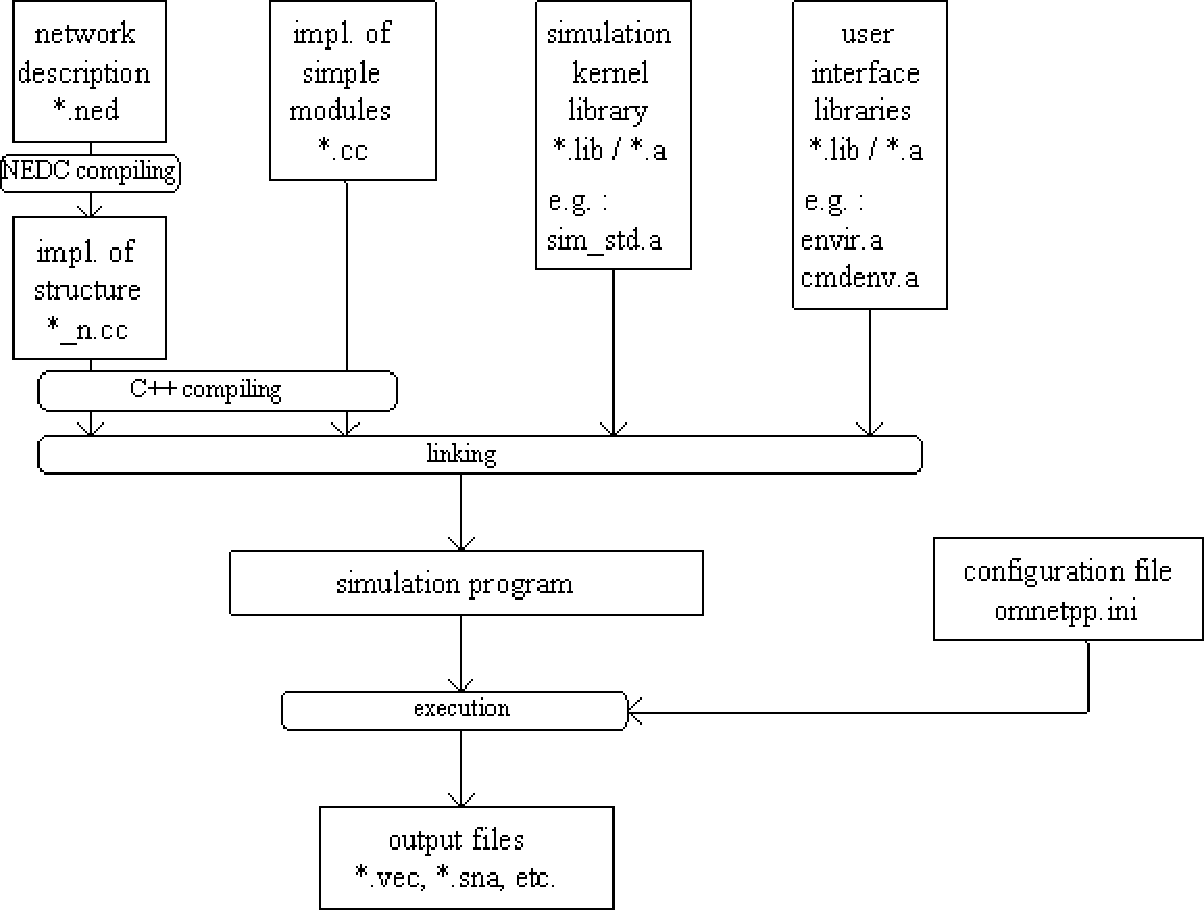
\includegraphics[width=5.992in, height=4.519in]{figures/usmanFig17}
    \caption{Building and running simulation}
  \end{center}
\end{figure}


This section discusses how to use the simulation system on the 
following platforms:
\begin{itemize}
  \item{Unix with gcc installed (and which is similar, Cygwin on Windows 
    NT)}
  \item{MSVC 6.0 on Windows NT}
  \item{Borland C++ 5.0 on Windows NT}
\end{itemize}




\section{Using Unix and gcc}

\subsection{Installation}

The installation process depends on what distribution you take 
(source, precompiled RPM, etc.) and it may change from release 
to release. The readme files in the distribution should give 
you enough (and up-to-date) guidance to go through the installation.





\subsection{Producing a makefile with the opp\_makemake script}

The \fprog{opp\_makemake} script can automatically generate the
makefile for your simulation program, based on the source files it
finds in your directory. \fprog{opp\_makemake} has several options,
the following command will display a summary:

\begin{Verbatim}
opp_makemake -h
\end{Verbatim}

To be able to use \fprog{opp\_makemake}, you have to collect all your 
sources (.ned, .cc, .h files) in one directory. (Large models 
which spread across several directories are covered later in 
this section.)


Then type 

\begin{Verbatim}
opp_makemake
\end{Verbatim}

This will create a file named Makefile\index{Makefile}. Thus if you
simply type make, your simulation program should build. The name of
the executable will be the same as the name of the directory
containing the files.


The freshly generated Makefile doesn't contain
dependencies\index{Makefile!dependencies}, it is advisable to add them
by typing \fprog[make]{make depend}. (You'll need a program named makedepend
for that, it's present on most Unix systems and in also Cygwin. The
warnings during the dependency generation process can be safely
ignored.)

In addition to the simulation executable, the makefile contains other
targets too. As mentioned, \fprog[make]{make depend} adds (or refreshes)
dependencies in the Makefile. \fprog[make]{make clean} deletes all files
that were produced by the make process. \fprog[make]{make re-makemake}
regenerates the makefile using \fprog[make]{opp\_makemake} (this is useful
if e.g.  after upgrading {\opp}, if \fprog{opp\_makemake} has
changed). \fprog[make]{make re-makemake-m} is similar to \fprog[make]{make
  re-makemake}, but it regenerates the Makefile.in file too (see
later).

If you already had a Makefile in that directory, \fprog{opp\_makemake}
will refuse overwriting it. You can force overwriting the old makefile
with the -f option:

\begin{Verbatim}
opp_makemake -f
\end{Verbatim}

If you have problems, check the path definitions (locations of include
files and libraries etc.) in the configure script\index{configure
  script} and correct them if necessary. Then re-run configure to
commit the changes to all makefiles, the \fprog{opp\_makemake} script
etc.


You can specify the user interface (Cmdenv/Tkenv) with the -u option
(with no -u, Tkenv is the default):

\begin{Verbatim}
opp_makemake -u Tkenv
\end{Verbatim}

The name of the output file\index{output!file} is set with the -o
option (the default is the name of the directory):

\begin{Verbatim}
opp_makemake -o fddi-net
\end{Verbatim}

If some of your source files are generated from other files (for
example, you use machine-generated NED files), write your make rules
into a file called makefrag. When you run \fprog{opp\_makemake}, it
will automatically insert makefrag into the resulting makefile.  With
the -i option, you can also name other files to be included into
Makefile.


If you want better portability for your models, you can generate
Makefile.in instead of Makefile with \fprog{opp\_makemake}'s -m
option. You can then use autoconf-like configure scripts to generate
the Makefile.





\subsection{Multi-directory models}

In the case of a large project, your source files may be spread across
several directories. You have to decide whether you want to use static
linking\index{static linking}, shared or run-time loaded (shared)
libraries\index{shared libraries}. Here we discuss static linking.


In each subdirectory (say trafgen/ and router/), run

\begin{Verbatim}
opp_makemake -n
\end{Verbatim}

The -n option means no linking is necessary, only compiling has 
to be done.


In your toplevel source directory, run

\begin{Verbatim}
opp_makemake trafgen/ router/
\end{Verbatim}

This results in recursive makefiles: when you build the simulation, make 
will descend into trafgen/ and router/, run make in both, then 
it will link an executable with the object files in the two directories.


You may need to use the -I option if you include files from other
directories. The -I option is for both C++ and NED
files\index{ned!include path}. In our example, you could run

\begin{Verbatim}
opp_makemake -n -I../router
\end{Verbatim}

in the trafgen/ directory and vice versa.


If you're willing to play with shared and run-time loaded libraries,
several \fprog{opp\_makemake} options and the
\texttt{[General]/load-libs=} ini file option leave you enough room to
do so.





\subsection{Static vs shared {\opp} system libraries}

Default linking uses the shared libraries\index{shared libraries}. One
reason you would want static linking is that
debugging\index{debugging} the {\opp} class library is more trouble
with shared libraries. Another reason might be that you want to run
the executable on another machine without having to worry about
setting the \fvar{LD\_LIBRARY\_PATH} variable (which should contain the name
of the directory where the {\opp} shared libraries are).

If you want static linking\index{static linking}, find the

\begin{Verbatim}
build_shared_libs=yes
\end{Verbatim}


line in the configure.user script and change it to

\begin{Verbatim}
build_shared_libs=no
\end{Verbatim}

Then you have to re-run the configure script and rebuild everything:

\begin{Verbatim}
./configure
make clean
make
\end{Verbatim}



\section{Using Win32 with MSVC}

\subsection{Prerequisite: install Tcl/Tk}

Download and install Tcl/Tk. You need at least version 8.0p1, 
but it's better to download the latest version.





\subsection{Installing {\opp}}

The installation process is not described here in detail. The 
readme files in the distribution should give you enough (and 
up-to-date) guidance to go through the installation.

What's important is that as the result of the installation, you 
should get the executables and the libraries in the bin/ and lib/ 
subdirectories within the top-level {\opp} directory.





\subsection{Building the samples from the MSVC IDE}

Unfortunately MSVC\index{MSVC} doesn't like the \texttt{.cc} extension, so first
you have to rename the \texttt{.cc} files to \texttt{.cpp}. You can do
that with samples/cc2cpp.bat.


Start the MSVC IDE and open the workspace (\texttt{.dsw}) file. Then
if you choose Build from the menu, the simulation executable should
build. If you encounter any problems, read the MSVC-related readme
file in the distribution -- it should contain more up-to-date
information than this manual.

\begin{sloppypar}
To change from Tkenv to Cmdenv or vica versa, choose Build{\textbar}Set 
active configuration from the menu and select one of 'Debug-Tkenv', 
'Release-Tkenv', 'Debug-Cmdenv', 'Release-Cmdenv', then re-link 
the executable.
\end{sloppypar}

If you have big models, you'll probably have to increase the stack
size. You'll find the setting under Project{\textbar}Settings
--\texttt{>} 'Link' tab --\texttt{>} choose 'Output' from combo
--\texttt{>} Stack allocations, Reserve. Be aware that if you don't
specify anything here, MSVC defaults to 1MB -- way too small.\\
If you need to modify the names of the Tcl/Tk libs (because you
installed a Tcl/Tk version other than 8.2), see
Project{\textbar}Settings --\texttt{>} 'Link' tab --\texttt{>} choose
'Input' from combo --\texttt{>} Libraries.

The Tcl/Tk install program normally sets the \fvar{TCL\_LIBRARY}
environment variable needed by Tcl applications. However, if you see
the ''can't find a usable init.tcl...'' error message when you start a
simulation program (or Gned or Plove), then that didn't happen and you
have to set the variable yourself.




\subsection{Creating project files for your simulations}

\begin{enumerate}
\item{Start by copying \& renaming one of the \texttt{.dsp} files from
    the samples directory. It already contains the Tkenv/Cmdenv
    configurations, etc.}
\item{ Rename all \texttt{.cc} files to \texttt{.cpp} (\texttt{ren
      *.cc *.cpp}) and add them to the project.}
\item{Add the \texttt{.ned} files to the project and set custom build
    option for them:

\begin{Verbatim}
Description: NED Compiling $(InputPath) 
Command: nedc -s _n.cpp $(InputPath)
Outputs: $(InputPath)_n.cpp
\end{Verbatim}
%% $


\textit{Hint: you can select all \texttt{.ned} files together, and
  'All configurations' from the combo at the left of the Settings
  dialog, and then you have to type this settings only once.}}


\item{For each \texttt{.ned} file, add a corresponding
    \texttt{\_n.cpp} file.
    
    \textit{Hint: if you compile the \texttt{.ned} files (choose
      'Compile' from the menu), the} \texttt{\_n.cpp} \textit{files will be
      created, and you can select them all at once in the 'Add files'
      dialog.}}
\item{Make sure to turn off exception handling\index{exception
      handling} and RTTI\index{RTTI} (they interfere with the
    coroutine library), and set the necessary reserved stack size.}
\item{Note: for Tkenv, link with \texttt{sim\_std.lib},
    \texttt{envir.lib}, \texttt{tkenv.lib} and the Tcl/Tk libraries
    (link as Win32 Console app...). For Cmdenv, you need to link with \texttt{sim\_std.lib}, \texttt{envir.lib}, and \texttt{cmdenv.lib}.\\
    It is planned to create wizards in the future to ease some of
    these steps.}
\end{enumerate}




\subsection{Using Plove}

If you want to use Plove\index{Plove}, you should download and install
Gnuplot\index{Gnuplot}.  You'll also need a couple of Unix tools like
\fprog{grep} and \fprog{awk}, the easiest way to get them is to
download and install the Cygwin package from
\href{http://www.cygnus.com}{www.cygnus.com}.  When you have
everything installed, start Plove and set the appropriate
configuration in Options{\textbar}External programs. If you entered
everything correctly, Plove should work.


A usual caveat is that Gnuplot expects forward slashes in filenames
and Plove supplies backslashes or vica versa (there are multiple
incompatible builds of Gnuplot on NT); if you suspect this might be
the problem, reverse the slash/backslash setting in
Options{\textbar}External programs.





\section{Hints for using Borland C++ and other compilers}

\subsection{Building {\opp}}

{\opp} currently doesn't support the Borland C++\index{Borland C++}.
This doesn't mean that the sources won't build (most probably they
will), but I am unable to maintain the respective makefiles.


However, the next sections contain some hints how to build simulation 
programs once you got the libraries compiled.





\subsection{Setting up a project file}

What you will need to have in your project file:
\begin{itemize}
  \item{your simple module C++ sources;}
  \item{your NED files\index{ned!files};}
  \item{for each NED file, the C++ file it will compile into (the
      \texttt{\_n.cc} file). Place the \texttt{.ned} file under the
      \texttt{\_n.cc} file in the project tree hierarchy.}
  \item{the {\opp} libraries: \texttt{sim\_std.lib},
      \texttt{envir.lib}, plus \texttt{cmdenv.lib} or
      \texttt{tkenv.lib}, depending on which user interface you want
      to link in. You also need the Tcl and Tk libraries if you're
      using Tkenv.}
\end{itemize}


The project options have to be set up like this:
\begin{itemize}
\item{Compile as a 32-bit flat console application. None of the
    special libraries (OWL, MFC, Class Library, OCF etc) are needed.}
\item{You have to turn off exception handling\index{exception
      handling}, it conflicts with the coroutine
    library\index{coroutine library} somehow. In the IDE:
    Options{\textbar}Project --\texttt{>} C++ Options --\texttt{>}
    Exception Handling/RTTI --\texttt{>} clear [ ] Enable exceptions.
    It must be done both when compiling the libraries and when
    compiling simulation applications.}
\item{Borland C++ does not recognize the \texttt{.cc} extension as
    C++. You have to teach it: Options{\textbar}Tools --\texttt{>}
    select CppCompile --\texttt{>} Edit --\texttt{>} Advanced
    --\texttt{>} add the \texttt{.cc} extension to the Translate From
    and Default For entries. Do the same with the EditText tool.}
\item{You also have to teach Borland C++ how to handle \texttt{.ned}
    files.  Select Options{\textbar}Tools --\texttt{>} New. Fill in
    the dialog as follows:
\begin{Verbatim}
  Name: NEDCompile

  Path: ..\..\src\nedc\nedc.exe

  Command Line: $NOSWAP $CAP MSG(BORL2MSG) $EDNAME

  Menu Text: NED Compile

  Help Hint: OMNeT++ NED compiler
\end{Verbatim}
%%$
  Select Advanced, and fill in the dialog:
\begin{Verbatim}
  Type: Translator
  Translate From:.ned
  Translate To:.cc
  Default For:.ned
  
\end{Verbatim}
}

\sloppy
\item{If you're going to build a LARGE model, be sure to
  increase the stack size\index{stack!size} in
  Options{\textbar}Project options{\textbar}Linker{\textbar}32-bit
  Linker{\textbar}Reserved stack size. The default is 0x1000000 (1MB),
  which is hardly enough for {\opp} simulations. Increase it to 64MB
  for example: 0x40000000. If the simulation exceeds the stack size
  configured here, you'll get nice exceptions, General Protection
  Faults and the like.}
\end{itemize}


%%% Local Variables: 
%%% mode: latex
%%% TeX-master: "usman"
%%% End: 

\cleardoublepage

\chapter{Running Simulations}
\label{cha:run-sim}

\section{Introduction}

This chapter describes how to run simulations. It covers basic usage,
user interfaces, batch runs, how to use Akaroa, and also explains
how to solve the most common errors.

\subsection{Running a Simulation Executable}
\label{sec:ch-run-sim:running}

By default, the output of an \fprog{opp\_makemake}-generated makefile is
a simulation executable that can be run directly. In simple cases,
this executable can be run without command-line arguments, but usually
one will need to specify options to specify what ini file to use,
which user interface to activate, where to load NED files from, and so on.

\subsubsection{Getting Help}

The following sections describe the most frequently used command-line
options. To get a complete list of supported command line options, run
the \fprog{opp\_run} command (or any other simulation executable) with
the \ttt{-h} option.

\begin{commandline}
$ opp_run -h
\end{commandline}

\subsubsection{Specifying Ini Files}

The default ini file is \ffilename{omnetpp.ini}, and is
loaded if no other ini file is given on the command line.

Ini files can be specified both as plain arguments and with the \ttt{-f}
option, so the following two commands are equivalent:

\begin{commandline}
$ ./fifo experiment.ini common.ini
$ ./fifo -f experiment.ini -f common.ini
\end{commandline}

Multiple ini files can be given, and their contents will be merged. This
allows for partitioning the configuration into separate files, for example
to simulation options, module parameters and result recording options.


\subsubsection{Specifying the NED Path}

NED files are loaded from directories listed on the NED path. More precisely,
they are loaded from the listed directories and their whole subdirectory trees.
Directories are separated with a semicolon (\ttt{;}).

\begin{note}
Semicolon is used as separator on both Unix and Windows.
\end{note}

The NED path can be specified in several ways:
\begin{itemize}
  \item using the \ttt{NEDPATH} environment variable
  \item using the \ttt{-n} command-line option
  \item in ini files, with the \fconfig{ned-path} configuration option
\end{itemize}

NED path resolution rules are as follows:

\begin{itemize}
  \item {\opp} checks for NED path specified on the command line with the \ttt{-n} option
  \item if not found on the command line, it checks for the NEDPATH environment variable
  \item the \fconfig{ned-path} option value from the ini file is appended to the result of the above steps
  \item if the result is still empty, it falls back to "." (the current directory)
\end{itemize}


\subsubsection{Selecting a User Interface}

{\opp} simulations can be run under different user interfaces.
Currently the following user interfaces are supported:

\begin{itemize}
  \item Tkenv: Tcl/Tk-based graphical, windowing user interface
  \item Cmdenv: command-line user interface for batch execution
\end{itemize}

You would typically test and debug your simulation under Tkenv,
then run actual simulation experiments from the command line or
shell script, using Cmdenv. Tkenv is also better suited for educational or
demonstration purposes.

Both Tkenv and Cmdenv are provided in the form of a library, and
you may choose between them by linking one or both into your
simulation executable. (Creating the executable was described in
chapter \ref{cha:building-simulation-programs}). Both user interfaces
are supported on Unix and Windows platforms.

You can choose which runtime environment is included in your simulation
executable when you generate your makefile. By default, both Tkenv and
Cmdenv is linked in so you can choose between them during runtime, but it
is possible to specify only a single user interface with the \ttt{-u
Cmdenv} or \ttt{-u Tkenv} option on the \fprog{opp\_makemake} command line.
This can be useful if you intend to run your simulations on a machine where
Tcl/Tk is not installed.

By default, Tkenv will be used if both runtime environments are present in
your executable. You explicitly select a user interface by adding the
\ttt{user-interface=Cmdenv} (or \ttt{=Tkenv}) option in your ini file, or
by specifying \ttt{-u Cmdenv} or \ttt{-u Tkenv} on the command line. If
both the config option and the command line option are present, the command
line option takes precedence.

\subsubsection{Selecting a Configuration and Run Number}

Configurations can be selected with the \ttt{-c <configname>} command line option.
If you do not specify the configuration and you are running under:

\begin{itemize}
  \item Tkenv: the runtime environment will prompt you to choose one.
  \item Cmdenv: the \ttt{General} configuration will be executed.
\end{itemize}

User interfaces may support the \ttt{-r runnumber} option to select runs,
either one or more, depending on the type of the user interface.

There are several command line options to get information about the iteration
variables and the number of runs in the configurations:

\begin{itemize}
  \item \ttt{-a} -- Prints all configuration names and the number of runs in them.
  \item \ttt{-x <configname>} -- Prints the number of runs available in the given configuration.
  \item \ttt{-g} -- Prints the unrolled configuration (together with the -x option) and
                    expands the iteration variables.
  \item \ttt{-G} -- Prints even more details than -g.
\end{itemize}


\subsubsection{Loading Extra Libraries}

{\opp} allows you to load shared libraries at runtime. This means that you can create
simulation models as a shared library and load the model later into a different executable without
the need to explicitly link against that library. This approach has several advantages.

\begin{itemize}
  \item It is possible to distribute the model as a shared library. Others may be able to use
  it without recompiling it.
  \item You can split a large model into smaller, reusable components.
  \item You can mix several models (even from different projects)
    without the need of linking or compiling.
\end{itemize}

Use the \ttt{-l libraryname} command line option to load a library dynamically.
{\opp} will attempt to load it using the \ffunc{dlopen()} or \ffunc{LoadLibrary()} functions and
automatically registers all simple modules in the library.

The prefix and suffix from the library name can be omitted (the extensions
\ttt{.dll}, \ttt{.so}, \ttt{.dylib}, and also the common \ttt{lib} prefix
on Unix systems). This means that you can specify the library name in a
platform independent way: if you specify \ttt{-l foo}, then {\opp} will
look for \ttt{foo.dll}, \ttt{libfoo.dll}, \ttt{libfoo.so} or \ttt{libfoo.dylib},
depending on the platform.

It is also possible to specify the libraries to be loaded in the ini file
with the \fconfig{load-libs} configuration option. The values from the command line
and the config file will be merged.

\begin{note}
  Runtime loading is not needed if your executable or shared lib was
  already linked against the library in question. In that case,
  the platform's dynamic loader will automatically load the library.
\end{note}

\begin{note}
  You must ensure that the library can be accessed by {\opp}. Either specify the
  library name with a full path (pre- and postfixes of the library file name
  still can be omitted), or adjust the shared library path environment variable
  of your OS (\ttt{PATH} on Windows, \ttt{LD\_LIBRARY\_PATH} on Unix, and
  \ttt{DYLD\_LIBRARY\_PATH} on Mac OS X.)
\end{note}

\subsection{Running a Shared Library}

Shared libraries can be run using the \fprog{opp\_run} program.
Both \fprog{opp\_run} and simulation executables are capable of
loading additional shared libraries; actually, \fprog{opp\_run}
is nothing else than an empty simulation executable.

Example:
\begin{commandline}
opp_run -l mymodel
\end{commandline}

The above example will load the model found in \ttt{libmymodel.so} and execute it.

\subsection{Controlling the Run}

There are several useful configuration options that control how a simulation is run.

\begin{itemize}
  \item \fconfig{cmdenv-express-mode} -- Provides only minimal status updates on the console.
  \item \fconfig{cmdenv-interactive} -- Allows the simulation to ask missing parameter values interactively
  \item \fconfig{cmdenv-status-frequency} -- Controls how often the status is written to the console.
  \item \fconfig{cpu-time-limit} -- Limits how long the simulation should run (in wall clock time)
  \item \fconfig{sim-time-limit} -- Limits how long the simulation should run (in simulation time)
  \item \fconfig{record-eventlog} -- Turns on the recording of the simulator events into an event log file.
           The resulting \ttt{.elog} file can be analyzed later in the IDE with the sequence chart tool.
  \item \fconfig{fingerprint} -- The simulation kernel computes a checksum while running the simulation.
          It is calculated from the module id and from the current simulation time of each event.
          If you specify the \fconfig{fingerprint} option in the config file, the simulation runtime will
          compare the computed checksum with the provided one. If there is a difference it will
          generate an error. This feature is very useful if you make some cosmetic changes to your
          source and want to be reasonable sure that your changes did not alter the behaviour
          of the model.
          \begin{warning}
          The value of the calculated fingerprint is heavily dependent on the accuracy of the floating
          point arithmetic. There are differences between the floating point handling of AMD and Intel CPUs.
          Running under a processor emulator software like \fprog{valgrind} may also produce
          a different fingerprint. This is normal. Hint: see gcc options \ttt{-mfpmath=sse -msse2}.
          \end{warning}
  \item \fconfig{debug-on-errors} -- If the runtime detects any error, it will generate a breakpoint
          so you will be able to check the location and the context of the problem in your debugger.
  \item \fconfig{debugger-attach-on-error} -- Controls just-in-time debugging. When this option is enabled
          and an error occurs during simulation, the simulation program will launch an external debugger,
          and have it attached to the simulation process. Related configuration options are
          \fconfig{debugger-attach-on-startup}, \fconfig{debugger-attach-command} and
          \fconfig{debugger-attach-wait-time}.
\end{itemize}

\begin{note}
  It is also possible to specify a configuration option on the command line (in which case the
  command line takes precedence). To do so, prefix the option name with a double
  dash (-{}-), and be sure not to have spaces around the equal sign. Example:
  \ttt{-{}-debug-on-errors=true}
\end{note}

To get the list of all possible configuration options, type:

\begin{commandline}
opp_run -h config
\end{commandline}


\section{Cmdenv: the Command-Line Interface}

The command line user interface\index{command line user interface} is
a small, portable and fast user interface that compiles and runs on
all platforms. Cmdenv\index{Cmdenv} is designed primarily for batch execution.

Cmdenv simply executes some or all simulation runs that are described
in the configuration file. If one run stops with an error message,
subsequent ones will still be executed. The runs to be executed can be
passed via command-line argument or in the ini file.

\subsection{Example Run}

When you run the Fifo example under Cmdenv, you should see
something like this:

\begin{commandline}
$ ./fifo -u Cmdenv -c Fifo1

OMNeT++ Discrete Event Simulation  (C) 1992-2008 Andras Varga, OpenSim Ltd.
Version: 4.0, edition: Academic Public License -- NOT FOR COMMERCIAL USE
See the license for distribution terms and warranty disclaimer
Setting up Cmdenv...
Loading NED files from .: 5

Preparing for running configuration Fifo1, run #0...
Scenario: $repetition=0
Assigned runID=Fifo1-0-20090104-12:23:25-5792
Setting up network 'FifoNet'...
Initializing...
Initializing module FifoNet, stage 0
Initializing module FifoNet.gen, stage 0
Initializing module FifoNet.fifo, stage 0
Initializing module FifoNet.sink, stage 0

Running simulation...
** Event #1   T=0   Elapsed: 0.000s (0m 00s)  0% completed
     Speed:     ev/sec=0   simsec/sec=0   ev/simsec=0
     Messages:  created: 2   present: 2   in FES: 1
** Event #232448   T=11719.051014922336   Elapsed: 2.003s (0m 02s)  3% completed
     Speed:     ev/sec=116050   simsec/sec=5850.75   ev/simsec=19.8351
     Messages:  created: 58114   present: 3   in FES: 2
...
** Event #7206882   T=360000.52066583684   Elapsed: 78.282s (1m 18s)  100% completed
     Speed:     ev/sec=118860   simsec/sec=5911.9   ev/simsec=20.1053
     Messages:  created: 1801723   present: 3   in FES: 2

<!> Simulation time limit reached -- simulation stopped.

Calling finish() at end of Run #0...
End.
\end{commandline}

As Cmdenv runs the simulation, it periodically prints the sequence number
of the current event, the simulation time, the elapsed (real) time,
and the performance of the simulation (how many events are processed per
second; the first two values are 0 because there wasn't enough data
for it to calculate yet). At the end of the simulation, the \ffunc{finish()}
methods of the simple modules are run, and the outputs from them are displayed.
On my machine this run took 34 seconds. This Cmdenv output can be
customized via \ffilename{omnetpp.ini} entries. The output file \ffilename{results/Fifo1-0.vec}
contains vector data recorded during simulation (here, queueing times),
and it can be processed using the IDE or other tools.

\subsection{Command-Line Options}

The command line environment allows you to specify more than one run by
using the \ttt{-r 2,4,6..8} format. See \ref{sec:ch-run-sim:batch-execution}
for more information about running simulation batches.

\subsection{Cmdenv Ini File Options}
\label{sec:ch-run-sim:cmdenv-section}

\fconfig{cmdenv-runs-to-execute} specifies which simulation runs should be executed.
It accepts a comma-separated list of run numbers or run number ranges, e.g.
\ttt{1,3..4,7..9}. If the value is missing, Cmdenv executes all runs that have
ini file sections; if no runs are specified in the ini file, Cmdenv does one run.
The \ttt{-r} command line option overrides this ini file setting.


Cmdenv can be executed in two modes, selected by the \fconfig{cmdenv-express-mode}
ini file option:

\begin{itemize}
    \item \tbf{Normal} (non-express) mode is for debugging; detailed information
        will be written to the standard output (event banners, module output,
        etc).
    \item \tbf{Express} mode can be used for long simulation runs; only
        periodical status updates are displayed about the progress of the
        simulation.
\end{itemize}

\fconfig{cmdenv-performance-display} affects express mode only: it controls
whether to print performance information. Turning it on results in a 3-line
entry printed on each update, containing ev/sec, simsec/sec, ev/simsec,
number of messages created/still present/currently scheduled in FES\index{FES}.

For a full list of options, see the options beginning with \ttt{cmdenv-} in
Appendix \ref{cha:config-options}.


\subsection{Interpreting Cmdenv Output}
\label{sec:ch-run-sim:interpreting-cmdenv-output}

When the simulation is running in ``express'' mode with detailed
performance display enabled, Cmdenv periodically outputs a three-line
status report about the progress of the simulation.
The output looks like this:

\begin{commandline}
...
** Event #250000   T=123.74354 ( 2m  3s)    Elapsed: 0m 12s
     Speed:     ev/sec=19731.6   simsec/sec=9.80713   ev/simsec=2011.97
     Messages:  created: 55532   present: 6553   in FES: 8
** Event #300000   T=148.55496 ( 2m 28s)    Elapsed: 0m 15s
     Speed:     ev/sec=19584.8   simsec/sec=9.64698   ev/simsec=2030.15
     Messages:  created: 66605   present: 7815   in FES: 7
...
\end{commandline}

The first line of the status display (beginning with \ttt{**})
contains:

\begin{itemize}
   \item{how many events have been processed so far}
   \item{the current simulation time (T), and}
   \item{the elapsed time (wall clock time) since the beginning of the simulation run.}
\end{itemize}

The second line displays info about simulation performance:

\begin{itemize}
   \item{\ttt{ev/sec} indicates \textit{performance}: how many events are processed
     in one real-time second.  On one hand it depends on your hardware
     (faster CPUs process more events per second), and on the other hand
     it depends on the complexity (amount of calculations) associated
     with processing one event. For example, protocol simulations tend to require
     more processing per event than e.g. queueing networks, thus
     the latter produce higher ev/sec values.
     In any case, this value is independent of the size (number of modules) in your model.}
   \item{\ttt{simsec/sec} shows \textit{relative speed} of the simulation, that is,
     how fast the simulation is progressing compared to real time, how many
     simulated seconds can be done in one real second. This value virtually depends
     on everything: on the hardware, on the size of the simulation model,
     on the complexity of events, and the average simulation time between events as well.}
   \item{\ttt{ev/simsec} is the \textit{event density}: how many events are
     there per simulated second. Event density only depends on the simulation model,
     regardless of the hardware used to simulate it: in a cell-level ATM simulation
     you will have very hight values ($10^9$), while in a bank teller simulation
     this value is probably well under 1. It also depends on the size of your
     model: if you double the number of modules in your model, you can expect
     the event density double, too.}
\end{itemize}

The third line displays the number of messages, and it is important
because it may indicate the `health' of your simulation.

\begin{itemize}
   \item{\ttt{Created}: total number of message objects created since the
     beginning of the simulation run. This does not mean that this many message
     object actually exist, because some (many) of them may have been deleted
     since then. It also does not mean that \textit{you} created all those
     messages -- the simulation kernel also creates messages for its own use
     (e.g. to implement \ttt{wait()} in an \ttt{activity()} simple module).}
   \item{\ttt{Present}: the number of message objects currently present
     in the simulation model, that is, the number of messages created (see above)
     minus the number of messages already deleted. This number includes
     the messages in the FES\index{FES}.}
   \item{\ttt{In FES}: the number of messages currently scheduled in the
     Future Event Set.}
\end{itemize}


The second value, the number of messages present, is more useful than
perhaps one would initially think. It can be an indicator of the `health' of the simulation;
if it is growing steadily, then either you have a memory leak and losing
messages (which indicates a programming error), or the network you simulate is
overloaded and queues are steadily filling up (which might indicate wrong input
parameters).

Of course, if the number of messages does not increase, it does not mean
that you do \textit{not} have a memory leak (other memory leaks are also
possible). Nevertheless the value is still useful, because by far the
most common way of leaking memory in a simulation is by not deleting messages.



\section{Tkenv: the Graphical User Interface}

Tkenv\index{Tkenv} is a portable graphical windowing user interface.
Tkenv supports interactive execution of the simulation, tracing and
debugging\index{simulation!debugging}. Tkenv is recommended in the
development stage of a simulation and for presentation purposes,
since it allows one to get a detailed picture of the state
of simulation at any point of execution and to follow what happens
inside the network.

\begin{note}
  This section only covers the command-line and configuration options
  of Tkenv; the user interface is described in the Tkenv chapter of the
  {\opp} User Guide.
\end{note}

\subsection{Command-Line and Configuration Options}

A simulation program built with Tkenv accepts all the general command line
options. \index{command line options} Additionally, the \ttt{-c configname}
and \ttt{-r runnumber} options can be used to preselect a single run for execution;
that is, these options suppress the initial run selection dialog.

Tkenv configuration options:
\begin{itemize}
  \item{\fconfig{tkenv-default-config}:
    Specifies which config Tkenv should set up automatically on startup. The
    default is to ask the user. This option is equivalent to the \ttt{-c}
    command-line option.}

  \item{\fconfig{tkenv-default-run}: Specifies which run (of the default
    config, see tkenv-default-config) Tkenv should set up automatically on startup.
    The default is to ask the user. This option is equivalent to the \ttt{-r}
    command-line option.}

  \item{\fconfig{tkenv-extra-stack}:
    Specifies the extra amount of stack that is reserved for each activity()
    simple module when the simulation is run under Tkenv.}

  \item{\fconfig{tkenv-image-path}: Specifies the path for loading module icons.}

  \item{\fconfig{tkenv-plugin-path}:
    Specifies the search path for Tkenv plugins. Tkenv plugins are .tcl files
    that get evaluated on startup.}
\end{itemize}

Tkenv-specific configuration options can also be specified on the command line
by prefixing them with two dashes (e.g \ttt{-{}-tkenv-option=value}). See
Appendix \ref{cha:config-options} for the list of possible configuration options.


\section{Batch Execution}
\label{sec:ch-run-sim:batch-execution}

Once your model works reliably, you will usually want to run several
simulations. You may want to run the model with various
parameter settings, or you may want \textit{(should want?)} to
run the same model with the same parameter settings but with
different random number generator seeds, to achieve statistically
more reliable results.

Running a simulation several times by hand can easily become tedious,
and then a good solution is to write a control script that
takes care of the task automatically. Unix shell is
a natural language choice to write the control script in,
but other languages like Perl, Matlab/Octave, Tcl, Ruby might also have
justification for this purpose.

Before running simulation batches, you must set a condition to
stop your simulation. This is usually a time limit set by the
\fconfig{sim-time-limit} configuration option, but you can limit your simulation
by using wall clock time (\fconfig{cpu-time-limit}) or by directly ending a
simulation with an API call if some condition is true.

\subsection{Using Cmdenv}

To execute more than one run using Cmdenv, use the \ttt{-r} option
and specify the runs in a comma separated format \ttt{1,2,4,9..11}, or you may leave
out the \ttt{-r} option to execute all runs in the experiment.

\begin{warning}
  Although it is very convenient, we do not recommend that you use this method for
  running simulation batches. Specifying more than one run number
  would run those simulations in the same process. This method is more prone to C++ programming
  errors. A failure in a single run may abort execution (segfault) or invalidate the results of subsequent runs. If you want
  to execute more than one run, we recommend that you run each of them in a separate process;
  you can use the \fprog{opp\_runall} program for this purpose.
\end{warning}


\subsection{Using Shell Scripts}

The following script executes a simulation named \ttt{wireless}
several times, with parameters for the different runs
given in the \ttt{runs.ini} file.

Before you execute your simulation batch, you may check how many
runs are available in the configuration you are using. Use the
\ttt{-x config} command line option to print the number of runs or
add the \ttt{-g} to get more details.

\begin{filelisting}
#! /bin/sh
./wireless -f runs.ini -r 1
./wireless -f runs.ini -r 2
./wireless -f runs.ini -r 3
./wireless -f runs.ini -r 4
...
./wireless -f runs.ini -r 10
\end{filelisting}

To run the above script, type it in a text file called e.g. \ttt{run},
give it \ttt{x} (executable) permission using \ttt{chmod},
then you can execute it by typing \ttt{./run}:

\begin{commandline}
$ chmod +x run
$ ./run
\end{commandline}

You can simplify the above script by using a \textit{for} loop.
In the example below, the variable \ttt{i} iterates through
the values of list given after the \ttt{in} keyword.
It is very practical, since you can leave out or add runs,
or change the order of runs by simply editing the list --
to demonstrate this, we skip run 6, and include run 15 instead.

\begin{filelisting}
#! /bin/sh
for i in 3 2 1 4 5 7 15 8 9 10; do
   ./wireless -f runs.ini -r $i
done
\end{filelisting}

If you have many runs, you can use a C-style loop:

\begin{filelisting}
#! /bin/sh
for ((i=1; $i<50; i++)); do
   ./wireless -f runs.ini -r $i
done
\end{filelisting}

\subsection{Using opp\_runall}

{\opp} has a utility program called \fprog{opp\_runall} which
allows you to execute a simulation batch in command line mode.
You must specify the whole command line you would use to run
your batch in Cmdenv. There are advantages to running your batches
this way:
\begin{itemize}
  \item Each simulation run executes in a separate operating system process.
        This means that a crash because of a programming error does not affect
        the outcome of the other runs. They are totally independent of each other.
  \item If you happen to have a multi core/processor machine, you can take advantage
        of the processing power by running sevaral runs in parallel.
\end{itemize}

The command basically creates a makefile which contains
a separate target for each run. By default the makefile will be executed causing each
target to run. You can give additional options to the \fprog{opp\_runall} command to
activate parallel building. The \ttt{-j} option can be used to specify the maximum number
of parallel runs allowed.

\begin{warning}
  Use the parallel execution option only if you have enough memory to run several simulations
  side by side. If you run out of memory your operating system will start swapping, and the overall
  performance of the system will be greatly reduced. Always specify the number of processes
  after the \ttt{-j} option, otherwise the \fprog{make} program will try to start \textit{all}
  runs at the same time. As a rule of thumb: if you have 4 cores (and enough memory), use \ttt{-j4}.
\end{warning}

The form of the command is:
\begin{commandline}
opp_runall -j2 ./aloha -u Cmdenv -c PureAlohaExperiment -r 0..23
\end{commandline}

You can use the \ttt{-x ConfigName -g} command line options with your simulation to
check the number of available runs.

Using the \ttt{-{}-export filename} option only generates the \ttt{makefile}, but does not start it.
You can run your batch later by invoking the generated makefile.

%% TODO
%%\subsection{Using Xgrid}


\section{Akaroa Support: Multiple Replications in Parallel}
\label{sec:ch-run-sim:akaroa}
\index{Akaroa}
\index{Multiple Replications in Parallel}

\subsection{Introduction}

Typical simulations are Monte-Carlo simulations: they use
(pseudo-)random numbers to drive the simulation model.
For the simulation to produce statistically reliable results,
one has to carefully consider the following:

\begin{itemize}
  \item{When the initial transient is over, when can we start
    collecting data? We usually don't want to include the
    initial transient when the simulation is still ``warming up.''}
  \item{When can we stop the simulation? We want to wait long enough
    so that the statistics we are collecting can ``stabilize'',
    or reach the required sample size to be statistically trustable.}
\end{itemize}

Neither question is trivial to answer. One might just suggest
to wait ``very long'' or ``long enough''. However, this is neither
simple (how do you know what is ``long enough''?) nor practical
(even with today's high speed processors simulations of modest complexity
can take hours, and one may not afford multiplying runtimes by,
say, 10, ``just to be safe.'') If you need further convincing,
please read \cite{Pawlikowsky02} and be horrified.

A possible solution is to look at the statistics while the simulation
is running, and decide at runtime when enough data have been
collected for the results to have reached the required accuracy.
One possible criterion is given by the confidence level,
more precisely, by its width relative to the mean.
But ex ante it is unknown how many observations have to be collected
to achieve this level -- it must be determined at runtime.


\subsection{What Is Akaroa}

Akaroa \cite{Akaroa99} addresses the above problem.
According to its authors, Akaroa (Akaroa2) is a ``fully automated
simulation tool designed for running distributed stochastic simulations
in MRIP scenario'' in a cluster computing environment.

MRIP stands for \textit{Multiple Replications in Parallel}.
In MRIP, the computers of the cluster run independent replications
of the whole simulation process (i.e. with the same parameters but
different seed for the RNGs (random number generators)),
generating statistically equivalent streams of simulation output data.
These data streams are fed to a global data analyser responsible for
analysis of the final results and for stopping the simulation
when the results reach a satisfactory accuracy.

The independent simulation processes run independently of one another
and continuously send their observations to the central analyser
and control process. This process \textit{combines} the independent data streams,
and calculates from these observations an overall estimate of the mean value
of each parameter.
Akaroa2 decides by a given confidence level and precision
whether it has enough observations or not. When it judges that is
has enough observations it halts the simulation.

If \textit{n} processors are used, the needed simulation execution time
is usually \textit{n} times smaller compared to a one-processor
simulation (the required number of observations are produced sooner).
Thus, the simulation would be sped up approximately in proportion
to the number of processors used and sometimes even more.

Akaroa was designed at the University of Canterbury in Christchurch, New Zealand
and can be used free of charge for teaching and non-profit research activities.


\subsection{Using Akaroa with {\opp}}

\subsubsection{Akaroa}

Before the simulation can be run in parallel under Akaroa, you have to
start up the system:

\begin{itemize}
  \item{Start \ttt{akmaster} running in the background on some host.}
  \item{On each host where you want to run a simulation engine,
     start \ttt{akslave} in the background.}
\end{itemize}

Each \ttt{akslave} establishes a connection with the \ttt{akmaster}.

Then you use \ttt{akrun} to start a simulation. \ttt{akrun} waits
for the simulation to complete, and writes a report of the results
to the standard output. The basic usage of the \ttt{akrun} command is:

\begin{commandline}
akrun -n num_hosts command [argument..]
\end{commandline}

where \textit{command} is the name of the simulation you want to start.
Parameters for Akaroa are read from the file named \ttt{Akaroa} in
the working directory. Collected data from the processes are
sent to the \ttt{akmaster} process, and when the required precision
has been reached, \ttt{akmaster} tells the simulation processes to
terminate. The results are written to the standard output.

The above description is not detailed enough help you
set up and successfully use Akaroa -- for that you need to read the
Akaroa manual.

\subsubsection{Configuring {\opp} for Akaroa}

First of all, you have to compile {\opp} with Akaroa support enabled.

The {\opp} simulation must be configured in \ffilename{omnetpp.ini}
so that it passes the observations to Akaroa. The simulation model itself does
not need to be changed -- it continues to write
the observations into output vectors (\cclass{cOutVector} objects,
see chapter \ref{cha:the-simulation-library}). You can place some of
the output vectors under Akaroa control.

You need to add the following to \ffilename{omnetpp.ini}:

\begin{inifile}
[General]
rng-class = "cAkaroaRNG"
outputvectormanager-class = "cAkOutputVectorManager"
\end{inifile}

These lines cause the simulation to obtain random numbers from Akaroa,
and allows data written to selected output vectors to be passed to Akaroa's
global data analyser.
    \footnote{For more details on the plugin mechanism these settings make use of,
    see section \ref{sec:ch-plugin-exts:customization}.}

Akaroa's RNG is a Combined Multiple Recursive pseudorandom
number generator (CMRG) with a period of approximately $2^{191}$
random numbers, and provides a unique stream of random numbers
for every simulation engine.

\begin{note}
It is vital that you obtain random numbers from Akaroa; otherwise,
all simulation processes will run with the same RNG seeds, and
produce exactly the same results.
\end{note}

Then you need to specify which output vectors you want to
be under Akaroa control (by default, none of them are).
You can use the \ttt{*}, \ttt{**} wildcards (see
section \ref{sec:ch-config-sim:wildcards}) to
place certain vectors under Akaroa control.

\begin{inifile}
<modulename>.<vectorname1>.with-akaroa = true
<modulename>.<vectorname2>.with-akaroa = true
\end{inifile}


\subsubsection{Using Shared File Systems}
\label{sec:run-sim:using-shared-filesystems}

It is usually practical to have the same physical disk mounted (e.g. via NFS or Samba)
on all computers in the cluster. However, because all {\opp} simulation
processes run with the same settings, they would overwrite each other's
output files (e.g. \ttt{omnetpp.vec}, \ttt{omnetpp.sca}).
Your can prevent this from happening using the
\fconfig{fname-append-host} ini file entry:

\begin{inifile}
[General]
fname-append-host = true
\end{inifile}

When turned on, it appends the host name to the names of the output
files (output vector, output scalar, snapshot files).



\section{Troubleshooting}

\subsection{Unrecognized Configuration Option}

If you receive an error message about unrecognized configuration
options you may use \ttt{-h config} or \ttt{-h configdetails} options
to display all possible configuration options and their descriptions.

\subsection{Stack Problems}

\subsubsection{``Stack violation (\textit{FooModule} stack too small?) in module \textit{bar.foo}''}
\index{stack!too small}

{\opp} detected that the module has used more stack space than it has
allocated. The solution is to increase the stack for that module type.
You can call the \ffunc{getStackUsage()} from \ffunc{finish()} to find out
actually how much stack the module used.


\subsubsection{``Error: Cannot allocate \textit{nn} bytes stack for module \textit{foo.bar''}}

The resolution depends on whether you are using {\opp} on Unix or on Windows.

\textbf{Unix.}
If you get the above message, you have to increase the total stack
size\index{stack!size} (the sum of all coroutine stacks). You can do
so in \ffilename{omnetpp.ini}:

\begin{inifile}
[General]
total-stack = 2MiB
\end{inifile}

There is no performance penalty if you set \fconfig{total-stack} too high. I
recommend to set it to a few K less than the maximum process stack
size allowed by the operating system (\fprog[ulimit]{ulimit -s}; see
next section).


\textbf{Windows.}
You need to set a \textit{low} (!) ``reserved stack size''
in the linker options, for example 64K (/stack:65536 linker flag) will do.
The ``reserved stack size'' is an attribute in the Windows exe
files' internal header. It can be set from the linker, or with
the \ttt{editbin} Microsoft utility. You can use the \ttt{opp\_stacktool}
program (which relies on another Microsoft utility called \ttt{dumpbin})
to display reserved stack size for executables.

You need a low reserved stack size because the Win32 Fiber API,
which is the mechanism underlying \ffunc{activity()}, uses
this number as the coroutine stack size, and with 1MiB being the default,
it is easy to run out of the 2GiB possible address space (2GiB/1MiB=2048).

A more detailed explanation follows.
Each fiber has its own stack, by default 1MiB (this is the ``reserved''
stack space -- i.e. reserved in the address space, but not the full
1MiB is actually ``committed'', i.e. has physical memory assigned to it).
This means that a 2GiB address space will run out after 2048 fibers,
which is way too few. (In practice, you won't even be able to create
this many fibers, because physical memory is also a limiting factor).
Therefore, the 1MiB reserved stack size (RSS) must be set to a smaller
value: the coroutine stack size requested for the module, plus
the \ttt{extra-stack-kb} amount for Cmdenv/Tkenv -- which makes
about 16K with Cmdenv, and about 48K when using Tkenv.
Unfortunately, the CreateFiber() Win32 API doesn't allow the RSS to be
specified. The more advanced CreateFiberEx() API which accepts RSS as
parameter is unfortunately only available from Windows XP.

The alternative is the stacksize parameter stored in the EXE header,
which can be set
via the STACKSIZE .def file parameter, via the /stack linker option,
or on an existing executable using the editbin /stack utility.
This parameter specifies a common RSS for the main program stack,
fiber and thread stacks. 64K should be enough. This is the way the
simulation executable should be created; linked with the /stack:65536
option, or the /stack:65536 parameter applied using editbin later.
For example, after applying the editbin /stacksize:65536 command to
dyna.exe, I was able to successfully run the Dyna sample with 8000
Client modules on my Win2K PC with 256M RAM (that means about 12000
modules at runtime, including about 4000 dynamically created modules.)


\subsubsection{``Segmentation fault''}

On Unix, if you set the total stack size higher, you may get a
segmentation fault during network setup\index{segmentation fault} (or
during execution if you use dynamically created modules), for exceeding
the operating system limit for maximum stack size. For example, in
Linux 2.4.x, the default stack limit is 8192K (that is, 8MiB). The
\fprog{ulimit} shell command can be used to modify the
resource limits, and you can raise the allowed maximum stack size
up to 64M.

\begin{commandline}
$ ulimit -s 65500
$ ulimit -s
65500
\end{commandline}

Further increase is only possible if you are root.
Resource limits are inherited by child processes.
The following sequence can be used under Linux to get a shell with
256M stack limit:

\begin{commandline}
$ su root
Password:
# ulimit -s 262144
# su andras
$ ulimit -s
262144
\end{commandline}

If you don't want to go through the above process at each login, you
can change the limit in the PAM configuration files. In Redhat Linux
(maybe other systems too), add the following line to
\ttt{/etc/pam.d/login}:

\begin{filelisting}
session    required    /lib/security/pam_limits.so
\end{filelisting}

and the following line to \ttt{/etc/security/limits.conf}:

\begin{filelisting}
*    hard    stack    65536
\end{filelisting}

\begin{sloppypar}
A more drastic solution is to recompile the kernel with a larger stack
limit. Edit \ttt{/usr/src/linux/include/linux/sched.h} and increase
\ttt{\_STK\_LIM} from \ttt{(8*1024*1024)} to \ttt{(64*1024*1024)}.
\end{sloppypar}

Finally, if you are tight with memory, you can switch to Cmdenv. Tkenv
increases the stack size of each module by about 32K\index{stack!for
  Tkenv} so that user interface code that is called from a
simple module's context can be safely executed.
Cmdenv does not need that much extra stack.


\subsubsection{Eventually...}

Once you get to the point where you have to adjust the total stack size to
get your program running, you should probably consider transforming (some
of) your \ffunc{activity()} simple modules to \ffunc{handleMessage()}.
\ffunc{activity()} does not scale well for large simulations.



\subsection{Memory Leaks and Crashes}

The most common problems in C++ are associated with memory allocation
(usage of \ttt{new} and \ttt{delete}):

\begin{itemize}
   \item{\textit{memory leaks,} that is, forgetting to delete objects
     or memory blocks no longer used;}
   \item{\textit{crashes,} usually due to referring to an already deleted
     object or memory block, or trying to delete one for a second time;}
   \item{\textit{heap corruption} (eventually leading to crash) due to
     overrunning allocated blocks, i.e. writing past the end of an allocated
     array.}
\end{itemize}

The most common cause of memory leaks in {\opp} simulations is
forgetting to delete messages. Both Tkenv and Cmdenv are able
to display the number of messages currently in the simulation,
helping you to determine if you have such a memory leak;
see section \ref{sec:ch-run-sim:interpreting-cmdenv-output}.
If you find that the number of messages is steadily increasing,
you need to find where the message objects are located. You can do so
by selecting \textit{Inspect|From list of all objects...} from
the Tkenv menu, and reviewing the list in the dialog that pops up.

If the number of messages is stable, it is still possible
you are leaking other \cclass{cOwnedObject}-based objects. You can
find them using Tkenv's \textit{Inspect|From list of all objects...}
function as well.

If you are leaking non-\cclass{cOwnedObject}-based objects or just
memory blocks (structs, arrays, etc., allocated by \ttt{new}),
you will not be able to find them via Tkenv. You will probably need
a specialized memory debugging tool like the ones described below.

\subsubsection{Memory Debugging Tools}

If you suspect that you may have memory allocation problems
(crashes associated with double-deletion or accessing already
deleted block, or memory leaks), you can use specialized tools
to track them down.

By far the most efficient, most robust and most versatile tool
is \textit{Valgrind}, originally developed for debugging KDE.

Other memory debuggers are \textit{NJAMD}, \textit{MemProf},
\textit{MPatrol}, \textit{dmalloc} and \textit{ElectricFence}.
Most of the above tools support tracking down memory leaks as well as
detecting double deletion, writing past the end of an allocated block, etc.

A proven commercial tool is \textit{Rational Purify}. It has
a good reputation and has proved its usefulness many times.

\subsection{Simulation Executes Slowly}

Check the following if you think your simulation is running too slowly:

\begin{itemize}
  \item Turn on express mode with the \ttt{cmdenv-express-mode=true} configuration option.
  \item Be sure that event logging is turned off (\ttt{record-eventlog=false} configuration option).
  \item Turn of vector file recording if you don't absolutely need it (\ttt{**.vector-recording=false}).
  \item If you are running under Tkenv, disable animation features, close inspectors,
        hide the timeline, hide object tree, turn off log filtering.
  \item Compile your code as release instead of debug (in some cases this can give you 5x speedup)
\end{itemize}


What can you do if the simulation executes much slower than you expect?
The best advice that can be given here is that you should
\tbf{use a good profiler} to find out how much time is spent in each
part of the program. Do not make the mistake of omitting this step,
thinking that you know which part is slow! Even for experienced
programmers, a profiling session is all too often full of surprises.
It often turns out that lots of CPU time is spent in completely
innocent-looking statements, while big and complex algorithms
don't take nearly as much time as you expected. \textit{Don't assume anything
-- profile before you optimize!}

A great profiler on Linux is the \textit{Valgrind}-based
\textit{callgrind}, and its visualizer \textit{KCachegrind}.
Unfortunately it won't be ported to Windows anytime soon.
On Windows, you are out of luck -- commercial products may help, or,
port your simulation to Linux. The latter goes usually much more smoothly
than one would expect.


%
%Use a profiler! KCachegrind.
%
%EV trick.
%
%Here are a few tips that can help you make the simulation faster:
%\begin{itemize}
%  \item{Use message subclassing instead of adding \ffunc{cPar}'s to messages.}
%  \item{Try to minimize message creations and deletions. Reuse
%    messages if possible.}
%  \item{Turn off the display of screen messages when you run the
%    simulation.  You can do this in the ini file. Alternatively, you
%    can place \ttt{\#ifdef}s around your \ttt{ev<<} and
%    \index{ev.printf()} calls and turn off the define when compiling
%    the simulation for speed.}
%  \item{Store the module parameters in local variables to avoid
%    calling \cclass{cPar} member functions every time.}
%\end{itemize}

%%% Local Variables:
%%% mode: latex
%%% TeX-master: "usman"
%%% End:

\cleardoublepage

\chapter{Result Recording and Analysis}
\label{cha:ana-sim}

\section{Result Recording}
\label{sec:ana-sim:result-recording}

{\opp} provides built-in support for recording simulation results, via
\textit{output vectors} and \textit{output scalars}. Output vectors are
time series data, recorded from simple modules or channels. You can use
output vectors to record end-to-end delays or round trip times of packets,
queue lengths, queueing times, module state, link utilization, packet
drops, etc. -- anything that is useful to get a full picture of what
happened in the model during the simulation run.

Output scalars are summary results, computed during the simulation and
written out when the simulation completes. A scalar result may be an
(integer or real) number, or may be a statistical summary comprised of
several fields such as count, mean, standard deviation, sum, minimum,
maximum, etc., and optionally histogram data.

Results may be collected and recorded in two ways:

\begin{enumerate}
  \item Based on the signal mechanism, using declared statistics;
  \item Directly from C++ code, using the simulation library
\end{enumerate}

The second method has been the traditional way of recording results. The
first method, based on signals and declared statistics, was introduced in
{\opp} 4.1, and it is preferable because it allows you to always record the
results in the form you need, without requiring heavy instrumentation or
continuous tweaking of the simulation model.

\subsection{Using Signals and Declared Statistics}
\label{sec:ana-sim:signals-and-statistics}

This approach combines the signal mechanism (see
\ref{sec:simple-modules:signals}) and NED properties (see
\ref{sec:ned-lang:properties}) in order to de-couple the generation of
results from their recording, thereby providing more flexibility in what to
record and in which form. The details of the solution have been described
in section \ref{sec:simple-modules:signal-based-statistics} in detail; here we
just give a short overview.

Statistics are declared in the NED files with the \ttt{@statistic} property,
and modules emit values using the signal mechanism. The simulation framework
records data by adding special result file writer listeners to the signals.
By being able to choose what listeners to add, the user can control what to
record in the result files and what computations to apply before recording.
The aforementioned section \ref{sec:simple-modules:signal-based-statistics}
also explains how to instrument simple modules and channels for signals-based
result recording.

The signals approach allows for calculation of aggregate statistics (such as the
total number of packet drops in the network) and for implementing a warm-up
period without support from module code. It also allows you to write
dedicated statistics collection modules for the simulation, also without
touching existing modules.

The same configuration options that were used to control result recording
with \cclass{cOutVector} and \ffunc{recordScalar()} also work when utilizing
the signals approach, and there are extra configuration options to make
the additional possibilities accessible.

\subsection{Direct Result Recording}
\label{sec:ana-sim:direct-result-recording}

With this approach, scalar and statistics results are collected in class
variables inside modules, then recorded in the finalization phase via
\ffunc{recordScalar()} calls. Vectors are recorded using
\cclass{cOutVector} objects. To record more details, like the
minimum/maximum value or the standard deviation, \cclass{cStdDev} and
\cclass{cWeightedStdDev} can be used, and for recording the distribution
there are histogram and other distribution estimation classes
(\cclass{cDoubleHistogram}, \cclass{cLongHistogram}, \cclass{cPSquare},
\cclass{cKSplit}, and others). These classes are described in sections
\ref{sec:sim-lib:statistics} and \ref{sec:sim-lib:result-recording}.
Recording of individual vectors, scalars and statistics can be enabled or
disabled via the configuration (ini file), and it is also the place to set
up recording intervals for vectors.

The drawback of recording results directly from modules is that result
recording is hardcoded in modules, and even simple requirement changes
(e.g. record the average delay instead of each delay value, or vice versa)
requires either code change or an excessive amount of result collection
code in the modules.



\section{Configuring Result Collection}
\label{sec:ana-sim:config-results}

\subsection{Result File Names}
\label{sec:ana-sim:result-file-names}

Simulation results are recorded into \textit{output scalar files} that
actually hold statistics results as well, and \textit{output vector
files}. The usual file extension for scalar files is \ttt{.sca}, and
for vector files \ttt{.vec}.

Every simulation run generates a single scalar file and a vector file.
The file names can be controlled with the \fconfig{output-vector-file}
and \fconfig{output-scalar-file} options. These options rarely need
to be used, because the default values are usually fine. The defaults
are:

\begin{inifile}
output-vector-file = "${resultdir}/${configname}-${runnumber}.vec"
output-scalar-file = "${resultdir}/${configname}-${runnumber}.sca"
\end{inifile}

Here, \ttt{\$\{resultdir\}} is the value of the \fconfig{result-dir}
configuration option which defaults to \ttt{results/}, and
\ttt{\$\{configname\}} and \ttt{\$\{runnumber\}} are the name of
the configuration name in the ini file (e.g. \ttt{[Config PureAloha]}),
and the run number. Thus, the above defaults generate file names
like \ttt{results/PureAloha-0.vec}, \ttt{results/PureAloha-1.vec},
and so on.

\begin{note}
  In {\opp} 3.x, the default result file names were \ttt{omnetpp.vec} and
  \ttt{omnetpp.sca}, and scalar files were always appended to, rather than
  being overwritten as in the 4.x version. When needed, the old behavior
  for scalar files can be turned back on by setting
  \ttt{output-scalar-file-append=true} in the configuration.
\end{note}


\subsection{Enabling/Disabling Result Items}
\label{sec:ana-sim:disabling-result-items}

The recording of simulation results can be enabled/disabled at multiple levels
with various configuration options:

\begin{itemize}
  \item All recording from a \fprop{@statistic} can be enabled/disabled together
        using the \fconfig{statistic-recording} option;
  \item Recording of a scalar or a statistic object can be controlled with the
        \fconfig{scalar-recording} option;
  \item Recording of an output vector can be controlled with the \fconfig{vector-recording}
        option;
  \item Recording of the bins of a histogram object can be controlled with the
        \fconfig{bin-recording} option.
\end{itemize}

All the above options are boolean per-object options, thus, they have similar syntaxes:

\begin{itemize}
\item \textit{<module-path>.<statistic-name>.}\fconfig{statistic-recording}\ttt{ = true/false}
\item \textit{<module-path>.<scalar-name>.}\fconfig{scalar-recording}\ttt{ = true/false}
\item \textit{<module-path>.<vector-name>.}\fconfig{vector-recording}\ttt{ = true/false}
\item \textit{<module-path>.<histogram-name>.}\fconfig{bin-recording}\ttt{ = true/false}
\end{itemize}

For example, all recording from the following statistic

\begin{ned}
@statistic[queueLength](record=max,timeavg,vector);
\end{ned}

can disabled with this ini file line:

\begin{inifile}
**.queueLength.statistic-recording = false
\end{inifile}

When a scalar, vector, or histogram is recorded using a \fprop{@statistic},
its name is derived from the statistic name, by appending the recording
mode after a semicolon. For example, the above statistic will generate 	the
scalars named \ttt{queueLength:max} and \ttt{queueLength:timeavg}, and the
vector named \ttt{queueLength:vector}. Their recording can be individually
disabled with the following lines:

\begin{inifile}
**.queueLength:max.scalar-recording = false
**.queueLength:timeavg.scalar-recording = false
**.queueLength:vector.vector-recording = false
\end{inifile}

The statistic, scalar or vector name part in the key may also contain
wildcards. This can be used, for example, to handle result items with
similar names together, or, by using \ttt{*} as name, for filtering by
module or to disable all recording. The following example turns off
recording of all scalar results except those called \ttt{latency}, and those
produced by modules named \ttt{tcp}:

\begin{inifile}
**.tcp.*.scalar-recording = true
**.latency.scalar-recording = true
**.scalar-recording = false
\end{inifile}

To disable all result recording, use the following three lines:

\begin{inifile}
**.statistic-recording = false
**.scalar-recording = false
**.vector-recording = false
\end{inifile}

The first line is not strictly necessary. However, it may improve runtime
performance because it causes result recorders not to be added, instead of
adding and then disabling them.


\subsection{Selecting Recording Modes for Signal-Based Statistics}
\label{sec:ana-sim:configuring-recording-modes}

Signal-based statistics recording has been designed so that it can be
easily configured to record a ``default minimal'' set of results, a
``detailed'' set of results, and a custom set of results (by modifying
the previous ones, or defined from scratch).

Recording can be tuned with the \fconfig{result-recording-modes}
per-object configuration option. The ``object'' here is the statistic,
which is identified by the full path (hierarchical name) of the module or
connection channel object in question, plus the name of the statistic
(which is the ``index'' of \fprop{@statistic} property, i.e. the name in
the square brackets). Thus, configuration keys have the syntax
\textit{<module-path>.<statistic-name>.}\ttt{result-recording-modes=}.

The \fconfig{result-recording-modes} option accepts one or more items as value,
separated by comma. An item may be a result recording mode (surprise!), and
two words with a special meaning, \ttt{default} and \ttt{all}:

\begin{itemize}
\item A \textit{result recording mode} means any item that may occur in the
      \ttt{record} key of the \fprop{@statistic} property; for example,
      \ttt{count}, \ttt{sum}, \ttt{mean}, \ttt{vector((count-1)/2)}.
\item \tbf{\ttt{default}} stands for the set of non-optional items from
      the \fprop{@statistic} property's \ttt{record} list, that is, those
      without question marks.
\item \tbf{\ttt{all}} means all items from the \fprop{@statistic} property's
      \ttt{record} list, including the ones with question marks.
\end{itemize}

The default value is \ttt{default}.

A lone ``-'' as option value disables all recording modes.

\textit{Recording mode} items in the list may be prefixed with ``+'' or
``-'' to add/remove them from the set of result recording modes. The
initial set of result recording modes is \ttt{default}; if the first item
is prefixed with ``+'' or ``-'', then that and all subsequent items are
understood as modifying the set; if the first item does not start with with
``+'' or ``-'', then it replaces the set, and further items are understood
as modifying the set.

This sounds more complicated than it is; an example will make it clear.
Suppose we are configuring the following statistic:

\begin{ned}
@statistic[foo](record=count,mean,max?,vector?);
\end{ned}

With the following the ini file lines (see results in comments):

\begin{inifile}
**.result-recording-modes = default  # --> count, mean
**.result-recording-modes = all      # --> count, mean, max, vector
**.result-recording-modes = -        # --> none
**.result-recording-modes = mean     # --> only mean (disables 'default')
**.result-recording-modes = default,-vector,+histogram # --> count,mean,histogram
**.result-recording-modes = -vector,+histogram         # --> same as the previous
**.result-recording-modes = all,-vector,+histogram  # --> count,mean,max,histogram
\end{inifile}

Here is another example which shows how to write a more specific option
key. The following line applies to \ttt{queueLength} statistics of
\ttt{fifo[]} submodule vectors anywhere in the network:

\begin{inifile}
**.fifo[*].queueLength.result-recording-modes = +vector  # default plus vector
\end{inifile}

In the result file, the recorded scalars will be suffixed with the recording mode,
i.e. the mean of \ttt{queueingTime} will be recorded as \ttt{queueingTime:mean}.


\subsection{Warm-up Period}
\label{sec:ana-sim:warmup-period}

The \fconfig{warmup-period} option specifies the length of the initial
warm-up period. When set, results belonging to the first $x$ seconds
of the simulation will not be recorded into output vectors, and will
not be counted into the calculation of output scalars.
This option is useful for steady-state simulations. The default is 0s
(no warmup period).

Example:

\begin{inifile}
warmup-period = 20s
\end{inifile}

Results recorded via signal-based statistics automatically obey the warm-up
period setting, but modules that compute and record scalar results
manually (via \ffunc{recordScalar()}) need to be modified so that they take
the warm-up period into account.

\begin{note}
When configuring a warm-up period, make sure that modules that compute and
record scalar results manually via \ffunc{recordScalar()} actually obey the
warm-up period in the C++ code.
\end{note}

The warm-up period is available via the \ffunc{getWarmupPeriod()} method of
the simulation manager object, so the C++ code that updates the corresponding
state variables needs to be surrounded with an \textit{if} statement:

Old:

\begin{cpp}
dropCount++;
\end{cpp}

New:

\begin{cpp}
if (simTime() >= getSimulation()->getWarmupPeriod())
    dropCount++;
\end{cpp}


\subsection{Output Vectors Recording Intervals}
\label{sec:ana-sim:vector-recording-intervals}

The size of output vector files can easily reach several gigabytes,
but very often, only some of the recorded statistics are
interesting to the analyst. In addition to selecting which vectors to
record, {\opp} also allows one to specify one or more collection intervals.

The latter can be configured with the \fconfig{vector-recording-intervals}
per-object option. The syntax of the configuration option is
\textit{<module-path>.<vector-name>.}\ttt{vector-recording-intervals=}\textit{<intervals>},
where both \textit{<module-path>} and \textit{<vector-name>} may
contain wildcards (see \ref{sec:config-sim:wildcards}).
\textit{<vector-name>} is the vector name, or the name string of the
\ffunc{cOutVector} object. By default, all output vectors are turned
on for the whole duration the simulation.

One can specify one or more intervals in the \textit{<startTime>..<stopTime>}
syntax, separated by comma. \textit{<startTime>} or \textit{<stopTime>} need
to be given with measurement units, and both can be omitted to denote
the beginning and the end of the simulation, respectively.

The following example limits all vectors to three intervals, except
\ttt{dropCount} vectors which will be recorded during the whole
simulation run:

\begin{inifile}
**.dropCount.vector-recording-intervals = 0..
**.vector-recording-intervals = 0..1000s, 5000s..6000s, 9000s..
\end{inifile}

\subsection{Recording Event Numbers in Output Vectors}
\label{sec:ana-sim:vector-eventnum-recording}

A third per-vector configuration option is \fconfig{vector-record-eventnumbers},
which specifies whether to record event numbers for an output vector.
(Simulation time and value are always recorded. Event numbers are needed
by the Sequence Chart Tool, for example.) Event number recording is enabled
by default; it may be turned off to save disk space.

\begin{inifile}
**.vector-record-eventnumbers = false
\end{inifile}

If the (default) \cclass{cIndexedFileOutputVectorManager} class is used to
record output vectors, there are two more options to fine-tune its resource
usage. \ttt{output-vectors-memory-limit} specifies the total memory that
can be used for buffering output vectors. Larger values produce less
fragmented vector files (i.e. cause vector data to be grouped into larger
chunks), and therefore allow more efficient processing later.
\ttt{vector-max-buffered-values} specifies the maximum number of values to
buffer per vector, before writing out a block into the output vector file.
The default is no per-vector limit (i.e. only the total memory limit is in
effect.)


\subsection{Saving Parameters as Scalars}
\label{sec:ana-sim:saving-parameters-as-scalars}

When you are running several simulations with different parameter
settings, you'll usually want to refer to selected
input parameters in the result analysis as well -- for example when
drawing a throughput (or response time) versus load (or network
background traffic) plot. Average throughput or response time numbers
are saved into the output scalar files, and it is useful for the input
parameters to get saved into the same file as well.

For convenience, {\opp} automatically saves the iteration variables
into the output scalar file if they have numeric value, so they can
be referred to during result analysis.

\begin{warning}
    If an iteration variable has non-numeric value, it will not be recorded
    automatically and cannot be used during analysis. This can happen
    unintentionally if you specify units inside an iteration variable list:
\begin{inifile}
**.param = exponential( ${mean=0.2s, 0.4s, 0.6s} )  #WRONG!
**.param = exponential( ${mean=0.2, 0.4, 0.6}s )    #OK
\end{inifile}
\end{warning}

Module parameters can also be saved, but this has to be
requested by the user, by configuring \ttt{param-record-as-scalar=true} for the
parameters in question. The configuration key is a pattern that
identifies the parameter, plus \ttt{.param-record-as-scalar}. An example:

\begin{inifile}
**.host[*].networkLoad.param-record-as-scalar = true
\end{inifile}

This looks simple enough, however there are three pitfalls:
non-numeric parameters, too many matching parameters, and
random-valued volatile parameters.

First, the scalar file only holds numeric results, so non-numeric
parameters cannot be recorded -- that will result in a runtime
error.

Second, if wildcards in the pattern match too many parameters, that
might unnecessarily increase the size of the scalar file. For example,
if the \ttt{host[]} module vector size is 1000 in the example below, then the
same value (3) will be saved 1000 times into the scalar file, once for
each host.

\begin{inifile}
**.host[*].startTime = 3
**.host[*].startTime.param-record-as-scalar = true  # saves "3" once for each host
\end{inifile}

Third, recording a random-valued volatile parameter will just save a
random number from that distribution. This is rarely what you need, and
the simulation kernel will also issue a warning if this happens.

\begin{inifile}
**.interarrivalTime = exponential(1s)
**.interarrivalTime.param-record-as-scalar = true  # wrong: saves random values!
\end{inifile}

These pitfalls are quite common in practice, so it is usually better
to rely on the iteration variables in the result analysis.
That is, one can rewrite the above example as

\begin{inifile}
**.interarrivalTime = exponential( ${mean=1}s )
\end{inifile}

and refer to the \ttt{\$mean} iteration variable instead of the
interarrivalTime module parameter(s) during result analysis.
\ttt{param-record-as-scalar=true} is not needed, because iteration variables are
automatically saved into the result files.


\subsection{Recording Precision}
\label{sec:ana-sim:outputfile-precision}

Output scalar and output vector files are text files, and floating point
values (\ttt{double}s) are recorded into it using \ttt{fprintf()}'s
\ttt{"\%g"} format. The number of significant digits can be configured
using the \fconfig{output-scalar-precision} and \fconfig{output-vector-precision}
configuration options.

The default precision is 12 digits. The following has to be considered when
setting a different value:

IEEE-754 doubles are 64-bit numbers. The mantissa is 52 bits, which is
roughly equivalent to 16 decimal places (52*log(2)/log(10)). However, due
to rounding errors, usually only 12..14 digits are correct, and the rest is
pretty much random garbage which should be ignored. However, when you
convert the decimal representation back into a \ttt{double} for result
processing, an additional small error will occur, because 0.1, 0.01, etc.
cannot be accurately represented in binary. This conversion error is
usually smaller than what that the \ttt{double} variable already had
before recording into the file. However, if it is important, you can
eliminate this error by setting the recording precision to 16 digits or
more (but again, be aware that the last digits are garbage). The practical
upper limit is 17 digits, setting it higher doesn't make any difference in
\ttt{fprintf()}'s output.

% To see finite machine precision and rounding errors, try this code:
%
% \ begin{verbatim}
% double x = 0.1;
% while (true)  {
%    printf("%.15g\n", x);
%    x = x + 0.1;
% }
% \ end{verbatim}
%
% The following, more advanced version will also print the error of
% converting back from text to double:
%
% \ begin{verbatim}
% double x = 0.1;
% while (true) {
%     char line[120];
%     sprintf(line, "%.15g \t%.14g \t%.13g \t%.12g", x, x, x, x);
%     double x15, x14, x13, x12;
%     sscanf(line, "%lg%lg%lg%lg", &x15, &x14, &x13, &x12);
%     printf("%s \t| %g  %g  %g  %g\n", line, (x15-x), (x14-x), (x13-x), (x12-x));
%     x = x + 0.1;
% }
% \ end{verbatim}
%    s
% For the complexity of the issue, see "What Every Computer Scientist
% Should Know About Floating-Point Arithmetic" by David Goldberg.

Errors resulting from converting to/from decimal representation can be
eliminated by choosing an output vector/output scalar manager class
which stores \ttt{double}s in their native binary form.
The appropriate configuration options are \fconfig{outputvectormanager-class}
and \fconfig{outputvectormanager-class}. For example,
\cclass{cMySQLOutputScalarManager} and \cclass{cMySQLOutputScalarManager}
provided in \ttt{samples/database} fulfill this requirement.

However, before worrying too much about rounding and conversion errors,
consider the \textit{real} accuracy of your results:

\begin{itemize}
  \item{in real life, it is very difficult to measure quantities (weight, distance,
     even time) with more than a few digits of precision. What precision
     are your input data? For example, if you approximate inter-arrival
     time as \textit{exponential(0.153)} when the mean is really
     \textit{0.152601...} and the distribution is not even exactly exponential,
     you are already starting out with a bigger error than rounding can cause.}

  \item{the simulation model is itself an approximation of real life. How much
     error do the (known and unknown) simplifications cause in the results?}
\end{itemize}

%% TODO also hint that results can be directed to database etc! by changing the implementation that cEnvir methods delegate to. (list cEnvir methods!)


\section{Overview of the Result File Formats}
\label{sec:ana-sim:result-file-formats}

Both output vector and scalar files are textual, line-oriented files.
The advantage of a text-based format is that it is very accessible
with a wide range of tools and languages. The format of result files is
documented in detail in Appendix \ref{cha:result-file-formats}.

%XXX move away:
%  \footnote{Recording is actually configurable, and one can record
%  results into a database as well, by writing appropriate result
%  manager classes and activating them in the configuration.}

By default, each file contains data from one run only.

Result files start with a header that contains several attributes of the
simulation run: a reasonably globally unique run ID, the network NED type
name, the experiment-measurement-replication labels, the values of
iteration variables and the repetition counter, the date and time, the host
name, the process id of the simulation, random number seeds, configuration
options, and so on. These data can be useful during result processing, and
increase the reproducibility of the results.

%%FIXME example header!

Vectors are recorded into a separate file for practical reasons: vector
data usually consume several magnitudes more disk space than scalars.

\subsection{Output Vector Files}
\label{sec:ana-sim:output-vector-files}

All output vectors from a simulation run are recorded into the same file.
The following sections describe the format of the file, and
how to process it.

An example file fragment (without header):

\begin{filelisting}
...
vector 1   net.host[12]  responseTime  TV
1  12.895  2355.66
1  14.126  4577.66664666
vector 2   net.router[9].ppp[0] queueLength  TV
2  16.960  2
1  23.086  2355.66666666
2  24.026  8
...
\end{filelisting}

There two types of lines: vector declaration lines (beginning with the word
\ttt{vector}), and data lines. A \textit{vector declaration line}
introduces a new output vector, and its columns are: vector Id, module of
creation, name of \cclass{cOutVector} object, and multiplicity (usually 1).
Actual data recorded in this vector are on \textit{data lines} which begin
with the vector Id. Further columns on data lines are the simulation time
and the recorded value.

% FIXME plus attribute lines!!! also event numbers

Since {\opp} 4.0, vector data are recorded into the file clustered by
output vectors, which, combined with index files, allows much more
efficient processing. Using the index file, tools can extract particular
vectors by reading only those parts of the file where the desired data are
located, and do not need to scan through the whole file linearly.


\subsection{Scalar Result Files}
\label{sec:ana-sim:scalar-result-files}

Fragment of an output scalar file (without header):

\begin{filelisting}
...
scalar "lan.hostA.mac" "frames sent"  99
scalar "lan.hostA.mac" "frames rcvd"  3088
scalar "lan.hostA.mac" "bytes sent"   64869
scalar "lan.hostA.mac" "bytes rcvd"   3529448
...
\end{filelisting}

Every scalar generates one \ttt{scalar} line in the file.

Statistics objects (\cclass{cStatictic} subclasses such as \cclass{cStdDev})
generate several lines: mean, standard deviation, etc.

%% FIXME TODO attributes, statistics example, etc

\section{The Analysis Tool in the Simulation IDE}
\label{sec:ana-sim:analysis-tool}

The Simulation IDE provides an Analysis Tool for analysis and visualization
of simulation results. The Analysis Tool lets you load several result files
at once, and presents their contents somewhat like a database. You can
browse the results, select the particular data you are interested in
(scalars, vectors, histograms), apply processing steps, and create various
charts or plots from them. Data selection, processing and charting steps
can be freely combined, resulting in a high degree of freedom.
These steps are grouped into and stored as "recipes", which get automatically
re-applied when new result files are added or existing files are
replaced. This automation spares the user lots of repetitive manual work,
without resorting to scripting.

The Analysis Tool is covered in detail in the User Guide.


\section{Scave Tool}
\label{sec:ana-sim:scavetool}
\index{scavetool}

Much of the IDE Analysis Tool's functionality is available on the command
line as well, via the \fprog{scavetool} program. \fprog{scavetool} is
suitable for filtering and basic processing of result files, and
exporting the result in various formats digestible for other tools.
\fprog{scavetool} has no graphics capabilities, but it can be used
to produce files that can be directly plotted with other tools like
gnuplot (see \ref{sec:ana-sim:gnuplot}).

When \fprog{scavetool} is invoked without arguments, it prints usage information:

\begin{commandline}
scavetool <command> [options] <file>...
\end{commandline}

\subsection{The \textit{filter} Command}
\label{sec:ana-sim:scavetool-filter-command}

The \textit{filter} command allows you to filter and/or convert result files.

A filter can be specified with the \textit{-p <filter>} option.
The filter is one or more \textit{<pattern>} or \textit{<fieldname>(<pattern>)}
expressions connected with \ttt{AND}, \ttt{OR} and \ttt{NOT} operators;
a naked \textit{<pattern>} is understood as \ttt{name(}\textit{<pattern>}\ttt{)}.
For example, the filter \ttt{"module(**.sink) AND name(delay)"} (or just
\ttt{"module(**.sink) AND delay"}) selects the \ttt{delay} vectors from all
\ttt{sink} modules.

The possible field names are:

\begin{itemize}
    \item\tbf{file}: full path of the result file
    \item\tbf{run}: run identifier
    \item\tbf{module}: module name
    \item\tbf{name}: vector name
    \item\tbf{attr:<runAttribute>}: value of an attribute of the run,
        e.g. \ttt{experiment}, \ttt{datetime} or \ttt{network}
    \item\tbf{param:<moduleParameter>}: value of the parameter in the run
\end{itemize}

Processing operations can be applied to vectors by the
\textit{-a <function>(<parameterlist>)} option. You can list
the available functions and their parameters with the \textit{info} command.

The name and format of the output file can be specified with the
\textit{-O <file>} and \textit{-F <formatname>} options, where
the format name is one of the following:

\begin{itemize}
    \item\tbf{vec}: vector file (default)
    \item\tbf{csv}: CSV file
    \item\tbf{octave}: Octave text file
    \item\tbf{matlab}: Matlab script file
\end{itemize}

The following example writes the window-averaged queuing times stored
in \ttt{in.vec} into \ttt{out.vec}:

\begin{commandline}
scavetool filter -p "queuing time" -a winavg(10) -O out.vec in.vec
\end{commandline}

The next example writes the queueing and transmission times of \ttt{sink}
modules into CSV files. It generates a separate file for each vector,
named \ttt{out-1.csv}, \ttt{out-2.csv}, etc.

\begin{commandline}
scavetool filter -p "module(**.sink) AND
                    (\"queueing time\" OR \"transmission time\")"
                 -O out.csv -F csv in.vec
\end{commandline}

The generated CSV files contain a header and two columns:

\begin{filelisting}
time,"Queue.sink.queueing time"
2.231807576851,0
7.843802235089,0
15.797137536721,3.59449
21.730758362277,6.30398
[...]
\end{filelisting}


\subsection{The \textit{index} Command}
\label{sec:ana-sim:scavetool-index-command}

If the index file was deleted or the vector file was modified, you need to
rebuild the index file before running the filter command:

\begin{commandline}
scavetool index Aloha-1.vec
\end{commandline}

Normally the vector data is written in blocks into the vector file.
However, if the vector file was generated by an older version of the
\cclass{cIOutputVectorManager}, it might not be so. In this case you have
to specify the -r option to rearrange the records of the vector file,
otherwise the index file would be too big and the indexing inefficient.

\subsection{The \textit{summary} Command}
\label{sec:ana-sim:scavetool-summary-command}

The \textit{summary} command reports the list of statistics names, module names,
run ids, configuration names in the given files to the standard output.

\begin{commandline}
scavetool summary Aloha-1.vec
\end{commandline}


\section{Alternative Statistical Analysis and Plotting Tools}
\label{sec:ana-sim:alternative-tools}

There are several programs and packages in addition to the {\opp} IDE
and \fprog{scavetool} that can also be used to analyze
simulation results, and create various plots and charts from them.

\begin{hint}
Our recommendation is GNU R because of its features, its popularity, and
the existence of an extension package written specifically for {\opp}
result processing.
\end{hint}


\subsection{GNU R}
\label{sec:ana-sim:gnu-r}
\index{GNU R}

R is a free software environment for statistical computing and graphics.
R has an excellent programming language and powerful plotting capabilities,
and it is supported on all major operating systems and platforms.

R is widely used for statistical software development and data analysis.
The program uses a command line interface, though several graphical user
interfaces are available.

\begin{hint}
An R package for {\opp} result processing is available from
\url{https://github.com/omnetpp/omnetpp-resultfiles/wiki}.
The package supports loading the contents of {\opp} result files into R,
organizing the data and creating various plots and charts.
The package is well documented, and the web site offers a Tutorial, a Tips
page, a tutorial for the Scalar Lattice GUI package, and other information.
\end{hint}

Several other {\opp}-related packages such as SimProcTC and Syntony already
use R for data analysis and plotting.


\subsection{NumPy, SciPy and MatPlotLib}
\label{sec:ana-sim:numpy-scipy-and-matplotlib}
\index{NumPy}\index{SciPy}\index{MatPlotLib}

NumPy and SciPy are numerical and scientific computing packages for the
Python programming language, and MatPlotlib is a plotting library (also for
Python).

MatPlotlib provides a ``pylab'' API designed to closely resemble that of
MATLAB, thereby making it easy to learn for experienced MATLAB users.
Matplotlib is distributed under a BSD-style license.


\subsection{MATLAB or Octave}
\label{sec:ana-sim:matlab-or-octave}
\index{Matlab}\index{Octave}

MATLAB is a commercial numerical computing environment and programming language.
MATLAB allows easy matrix manipulation, plotting of functions and data,
implementation of algorithms, creation of user interfaces, and interfacing
with programs in other languages.

Octave is an open-source Matlab-like package, available on nearly all platforms.
Currently Octave relies on Gnuplot for plotting, and has more limited
graphics capabilities than GNU R or MATLAB.


\subsection{Gnuplot}
\label{sec:ana-sim:gnuplot}
\index{Gnuplot}

Gnuplot is a very popular command-line program that can generate two-
and three-dimensional plots of functions and data. The program runs
on all major platforms, and it is well supported.

Gnuplot has an interactive command interface. For example, if you have
the data files \texttt{foo.csv} and \texttt{bar.csv} that contain
two values per line ($x$ $y$; such files can be exported with
\fprog{scavetool} from vector files), you can plot them in the same
graph by typing:

\begin{commandline}
plot "foo.csv" with lines, "bar.csv" with lines
\end{commandline}

To adjust the $y$ range, you would type:

\begin{commandline}
set yrange [0:1.2]
replot
\end{commandline}

Several commands are available to adjust ranges, plotting style, labels,
scaling etc. On Windows, you can copy the resulting graph to the clipboard from
the Gnuplot window's system menu, then insert it into the application you
are working with.


\subsection{ROOT}
\label{sec:ana-sim:root}
\index{ROOT}

\textit{ROOT} is an object-oriented data analysis framework,
with strong support for plotting and graphics in general.
ROOT was developed at CERN, and is distributed under a BSD-like license.

ROOT is based on \textit{CINT}, a ``C/C++ interpreter''
aimed at processing C/C++ scripts. It is probably harder to get started
using ROOT than with either Gnuplot or Grace, but you will find that ROOT provides
power and flexibility that would be unattainable with the other two programs.


\subsection{Grace}
\label{sec:ana-sim:grace}
\index{Grace}

An ``honorable mention,'' \textit{Grace} is a powerful GPL data visualization
program with a menu-and-dialog graphical user interface for X and Motif. It
has also been ported to Windows. Grace is also known as \textit{xmgrace},
and it is a successor of \textit{ACE/gr} or \textit{Xmgr}.

Grace can export graphics in various raster and vector formats, and has
many useful features like built-in statistics and analysis functions (e.g.
correlation, histogram), fitting, splines, etc., and it also has a built-in
programming language.


\subsection{Spreadsheet Programs}
\label{sec:ana-sim:spreadsheet-programs}
\index{Spreadsheets}

One straightforward solution is to use spreadsheets such as OpenOffice
Calc, Microsoft Excel, Gnumeric or Calligra Tables (formerly KSpread).
Data can be imported from CSV or other formats, exported with \fprog{scavetool}
(see \ref{sec:ana-sim:scavetool}).

Spreadsheets have good charting and statistical features. A useful
functionality spreadsheets offer for analyzing scalar files is
\textit{PivotTable} (Excel) or \textit{DataPilot} (OpenOffice). The
drawback of using spreadsheets is limited automation, leading to tedious
and repetitive tasks; also, the number of rows is usually limited to about
32,000..64,000, which can be limiting when working with large vector files.


%%% Local Variables:
%%% mode: latex
%%% TeX-master: "usman"
%%% End:



\cleardoublepage

\chapter{Parallel Execution}
\label{cha:parallel-execution}

\section{{\opp} support for parallel execution}

\subsection{Introduction to Parallel Discrete Event Simulation}

{\opp} supports parallel execution\index{parallel execution} of large
simulations. The following paragraphs provide a very brief (and thus
not very accurate) picture of the problems and methods of parallel
discrete event simulation (PDES\index{PDES}). Interested readers --
and those who are thinking about doing PDES with {\opp} -- are
strongly encouraged to look into the literature.


For parallel execution, the model is to be partitioned to several
segments that will be simulated independently on different hosts or
processors. Each segment will have its own local Future Event Set,
thus they will maintain local simulation times. The main issue with
parallel simulations is keeping segments synchronized in order to
avoid violating causality of events. Without synchronization, a
message sent by one segment could arrive in another segment when the
simulation time in the receiving segment has already passed the
timestamp (arrival time) of the message. This would break
causality\index{event!causality} of events in the receiving segment.

There are mainly three different methods used for synchronizing 
segments:
\begin{enumerate}
  \item{\textbf{Conservative synchronization}\index{conservative
      synchronization} exploits knowledge about when segments send
    messages to other segments, and uses 'null' messages to propagate
    this info to other segments. This may speed up simulation, since
    e.g. if a segment knows it won't receive any messages from other
    segments until $t+\Delta t$ simulation time, it may advance until
    $t+\Delta t$ without the need for external synchronization.
    Conservative syncronization requires modifications to existing
    models, i.e., inserting code which sends out the 'null' messages.
    Conservative simulation tends to converge to sequential simulation
    (slowed down by communication between segments) if there's not
    enough parallelism in the model, or parallelism is not exploited
    by sending enough 'null' messages.}
  
  \item{\textbf{Optimistic synchronization}\index{optimistic
      synchronization} allows incausalities to occur, but detects and
    repairs them. Repairing involves rollbacks to a previous state,
    sending out anti-messages to cancel messages sent out during the
    period that is being rolled back, etc.  Optimistic synchronization
    is extremely difficult to implement, because it requires periodic
    state saving and the ability to restore previous states. In any
    case, implementing optimistic synchronization in {\opp} would
    require -- in addition to a more complicated simulation kernel --
    writing significantly more complex simple\index{module!simple}
    module code from the user.  Optimistic synchronization may be slow
    in cases of excessive rollbacks.}
  
  \item{\textbf{Statistical synchronization}\index{statistical
      synchronization} is a compromise where segments do not exchange
    individual messages but distributions of the traffic flow
    characteristics. While conservative and optimistic synchronization
    are exact methods (they produce exactly the same results as the
    corresponding sequential simulation would), this is certainly not
    true for statistical synchronization where the results may contain
    error introduced by the statistical nature of the synchronization.
    Statistical synchronization does not require changes to existing
    models, only the insertion of extra modules, called
    \textit{''statistical interfaces''}, therefore it is significantly
    easier to implement than either conservative or optimistic. In
    addition to easier implementation, there is a potential for much
    larger speedup than with conservative or optimistic, because the
    method is much less sensitive to communication delay between
    processors running the segments. Therefore, for parallel
    simulation on a cluster of workstations, statistical
    synchronisation may be the only feasible method.}
\end{enumerate}





\subsection{{\opp} support for parallel simulation}

The simulation kernel makes it possible to send messages from one
segment to another. A message can contain arbitrarily complex data
structures; these are transferred transparently, even between hosts of
different architectures. The simulation kernel provides a simple
synchronization mechanism (\textit{syncpoints}, available through the
\fname{syncpoint()} call) that can ensure that causality is kept when
sending messages between segments. Syncpoints correspond to
\textit{null messages} found in the literature.

Message sending and syncpoints enable one to implement conservative 
PDES and also Statistical Synchronization. The simulation class 
library contains objects that explicitly support the implementation 
of models using Statistical Synchronization.


High level debugging is supported by saving the textual output 
from remote segments to a log file and/or relaying them to a 
single console.

{\opp} supports flexible partitioning of the
model\index{model!partitioning}. In the NED language, by using
\textit{machine parameters} you can specify \textit{logical
  hosts}\index{logical hosts} for different modules at any level of
the module hierarchy of the network. You map logical hosts to physical
ones in the ini file; if you map several logical hosts into the same
physical machine, they will be merged into a single {\opp} process.


One may choose between using the MPI\index{MPI} (Message Passing
Interface) and the PVM3\index{PVM} (Parallel Virtual Machine Version
3) libraries for communication between hosts. Both libraries are
portable and widely used in university and research environments. MPI
is newer though and considered to be the successor of PVM. You can
find MPI and PVM readings in the Reference.





\subsection{Syncpoints}

\textbf{Overview}


When running a simulation in parallel, different segments of 
the model execute as independent UNIX processes, typically on 
separate hosts. Since the hosts can be of different speed and 
the simulated model segments can be of different complexity, 
at a given moment the model times of different segments will 
differ: some segments are ahead of the others and some lag behind. 
Suppose that a message is sent from segment A to segment B which 
is ahead of A in model time. If B processed the message, causality 
would break. This should never happen.


The solution built in {\opp} is the following. Segment A must know in
advance when it will send the next message to segment B and announce
it with the \fname{syncpoint()} call. The simulation kernel sends the
syncpoint to segment B. When segment B's model time reaches the
specified time, segment B's simulation kernel blocks execution until
the promised message arrives from A. Then the simulation continues,
typically but not necessarily with the message that has just been
received from A.

In the reverse case when A is ahead of B, A's message arrived at B
before it has reached the syncpoint. In this case, there is no problem
and the syncpoint is just an unnecessary precaution. B just inserts
the message in its future event set, clears the syncpoint and
continues execution.


\textbf{The syncpoint API}


The \fname{syncpoint()} call takes two arguments. The first is the
model time when (or more precisely: when of after when) the simple
module will send a message to another simple module in a different
segment. The second argument is a gate given with its number or its
name. The gate implicitly specifies the destination segment to
synchronize with.

\begin{Verbatim}
syncpoint(t, "outgate");
\end{Verbatim}


\textbf{Details of the syncpoint implementation}


If the destination module is in the same segment, the call is ignored.
(This makes it possible to run models designed to execute in parallel
as a single process, without any modification.) Each segment keeps a
list of syncpoints sent to it (time + gate), ordered by time.
Simulation executes normally until it comes to an event that has a
time \textit{definitely past} the first syncpoint in the list. That
event is not processed, but the segment goes into a blocked state.
While the segment is blocked, it listens for messages arriving from
other segments. (In the actual implementation, passive wait is used so
a blocked segment doesn't use much CPU time.) Each message that
arrives deletes the first syncpoint in the list that matches its gate.
The segment goes out of the blocked state when -- because of deletions
-- the first syncpoint in the list is no longer past the event in
question. Then the simulation goes on normally, either with the newly
arrived message (or the earliest of them) or the original event. A
message that arrives outside of the blocked state also causes deletion
of the first matching syncpoint in the list; this case corresponds to
the reverse case when the sender segment is ahead of the receiving
segment in model time.


\textbf{Deadlock}


It is possible to cause deadlock\index{parallel simulation!deadlock}
with carelessly placed syncpoints.  Suppose that segment A declares a
syncpoint at 10s with segment B, but it will actually send a message
only at 10.5s. If segment B does the same to segment A, a nice
deadlock is created. {\opp} makes no effort to detect or prevent such
deadlocks; it is entirely the simulation programmer's task to take
care that deadlocks do not occur.




\section{Configuring a simulation for parallel execution}

\subsection{Configuring {\opp}}

\subsubsection{Choosing between MPI and PVM}


You have let {\opp} know if you want to use MPI\index{MPI} or
PVM\index{PVM}. This can be configured in the \texttt{[General]}
section of the ini file, via te
\fpar[parallel-system]{parallel-system=} entry. Its value can be
''PVM'' or ''MPI''; it defaults to ''MPI''.

\begin{Verbatim}[commandchars=\\\{\}]
; file: omnetpp.ini
;...
\textbf{[General]}
parallel-system = MPI
\end{Verbatim}


\subsubsection{Mapping logical machines to physical ones}

The \fpar[ned!keywords!on]{on:} phrases in the NED descriptions
specify the logical machine(s) on which the module is run. The machine
parameters are mapped to physical machines in the \texttt{[Machines]}
section of the configuration file:

\begin{Verbatim}[commandchars=\\\{\}]
; file: omnetpp.ini
;...
\tbf{[Machines]}
node1 = whale.hit.bme.hu
node4 = whale.hit.bme.hu
node2 = puppis.hit.bme.hu
node3 = dolphin.hit.bme.hu
;...
\end{Verbatim}


\subsubsection{Configuration of the slaves}

Slave processes can be configured in the \texttt{[Slaves]} section of
the configuration file:

\begin{Verbatim}[commandchars=\\\{\}]
; file: omnetpp.ini
\textbf{[Slaves]}
write-slavelog=
slavelog-file=
module-messages=
errmsgs-to-console=
infomsgs-to-console=
modmsgs-to-console=
\end{Verbatim}

Screen input/output of the slaves is re-routed to the console.
However, any file I/O is done in the local file system of each host.



\subsection{Setting up PVM}

\subsubsection{The PVM virtual machine}


The \ttt{pvmhosts} file is used by PVM to describe what computers will
participate in the virtual machine, where the executables (in our
case, the {\opp} programs) are located on each computer, what working
directories should be set etc.


It is advisable to have a common, shared directory mounted on all
participating hosts; this eliminates the tedious work of having to
copy files to all hosts again and again.


If using {\opp}, it is a good idea to write separate \texttt{pvmhosts}
files for each simulation program. Since simulation programs are
typically in separate directories, the \texttt{pvmhosts} file in each
directory can name that directory as executables directory and working
directory for each host. This way, there is no need to create soft
links or explicitly name directories in the {\opp} ini files.


Each line in the \texttt{pvmhosts} file describes one host. An example
line (this all should be a \textit{single line}!):

\begin{Verbatim}
whale ip=whale.hit.bme.hu lo=andras
   dx=/home/andras/pvm/pvm
   ep=/home/andras/omnetpp/projects/fddi
   wd=/home/andras/omnetpp/projects/fddi
\end{Verbatim}

To start PVM with this configuration:

\begin{Verbatim}
cd ~/omnetpp/projects/fddi
pvm pvmhosts
\end{Verbatim}

\subsubsection{Configuration and running}

The user must have PVM installed on the hosts he is going to 
run segments on.


To set up a simulation for distributed execution, the user must:
\begin{enumerate}
\item{set the \fvar{PVM\_ROOT} environment variable}
\item{link the simulation executable with \ttt{sim\_pvm} instead of
  \ttt{sim\_std} (You can do it by setting \fvar{PVM\_SUPPORT} to
  \ttt{yes} in a \fprog{opp\_makemake}-generated makefile.)}
\item{set \ttt{distributed=true} in the \ttt{[General]} section of the
  configuration file.}
\item{specify the logical-hosts-to-physical-machines mapping in the
  \ttt{[Machines]} section}
\item{copy the simulation executable and the configuration file to
  each host if they have physically different disks}
\item{start \ttt{pvm} with an appropriate \ttt{pvmhosts} file}
\item{start the simulation executable on the host which is supposed to
  be the console. That process will start up the program on the other
  hosts too and do the simulation.}
\end{enumerate}

The first machine is called ''console'' or ``master'', the 
others are called ``slaves''.


\subsubsection{If there are problems...}


PVM programs in general are more difficult to get running than 
ordinary programs. Wrong settings in the PVM configuration files 
can cause various problems, for example. Also, parallel programs 
are a lot harder to test and debug.


What can you do if your distributed {\opp} simulation won't 
work?
\begin{itemize}
  \item{First of all, check the \ttt{pvmhosts} file to see if PVM
    looks for the executables in the right directories on all hosts
    and the working directories are right (typically, the same
    directory as the executable's).}
  \item{In the ini file, enable writing the \ttt{slave.log} files for
    the slave processes and check what is written into them.}
  \item{You can try enabling the \fdef{SINGLE\_HOST} define in the
    \ttt{sim/pvm/pvmmod.cc} source file. This will make {\opp} run all
    segments of the distributed simulation on the local host, making
    things a lot easier to manage. }
  \item{Also, try the defining \fdef{PVM\_DEBUG} at the same place: it
    enables a lot of \fname{ev.printf()}s in the code interfacing with
    PVM, so it is easier to spot where the problems are.}
  \item{PVM itself also has an environment variable which, if set,
    causes the PVM library to print out debugging information.
    However, this is very low-level information, it will rarely be
    useful.}
\end{itemize}




\subsection{Setting up MPI}

TBD\dots \\





\section{Statistical synchronization}
\begin{sloppypar}
\subsection{The description of the Statistical Synchronization Method (SSM)}
\end{sloppypar}

Similarly to other parallel discrete event simulation methods, the
model to be simulated - which is more or less a precise representation
of a real system - is divided into segments, where the segments
usually describe the behaviour of functional units of the real system.
The communication of the segments can be represented by sending and
receiving various messages. The simulators of the segments are
executed by separate processors.


The communication of these segments is simulated with appropriate
interfaces. The messages generated in a given segment and to be
processed in a different segment are not transmitted there, but the
output interfaces collect the statistical data of them.  If the input
interfaces generate messages for the segments according to the
statistical characteristics of the messages collected by the proper
output interfaces, the segments with their input- and output
interfaces can be simulated separately, giving statistically correct
results. The events in one segment have not the same effect in other
segments as in the original model, so the results collected during the
SSM\index{SSM} are not exact. The precision depends on the
segmentation, on the accuracy of statistics collection and
regeneration, and on the frequency of the statistics exchange among
the processors.


\textbf{Segmentation}


The segments of the simulator\index{simulation!parallel segments} are
executed by separate processors, they have their own, independent
virtual times. Because the interactions among segments are performed
by the statistical parameters of these interactions, the segmentation
should be done so, that the overwhelming majority of the interactions
should happen within the segments and not among them. This speeds up
the so-called inter-segment transients\index{inter-segment transients}
and improves the accuracy as well.


\textbf{Timing of statistics exchange}


Asynchronous statistics exchange\index{statistic!asynchronous
  exchange} means, that whenever a statistical result collection in an
output interface is ready, it is applied - after mapping and
correction - in the proper input interface.  This is clearly more
efficient, than the so-called synchronous statistics
exchange\index{statistic!synchronous exchange}, which means, that we
delay the application of collected values until all the output
interfaces get ready with the result collection. Frequent statistics
exchange makes the inter-segment transient faster, but the lower
sample numbers makes the estimation - and the whole simulation - less
precise.


To learn more about SSM, see [PON92] and [PON93].





\subsection{Using SSM in {\opp}}

{\opp} directly supports the implementation of statistical
interface\index{statistical interface} with the following classes:

\cclass{cLongHistogram}, \cclass{cDoubleHistogram}, \cclass{cPSquare}, \cclass{cPar}.


%%% Local Variables: 
%%% mode: latex
%%% TeX-master: "usman"
%%% End: 

\cleardoublepage

\chapter{Customization and Embedding}
\label{cha:opp-design}

\section{Architecture}

{\opp} has a modular architecture. The following diagram shows the
high-level architecture of {\opp} simulations:

\begin{figure}[htbp]
  \begin{center}
    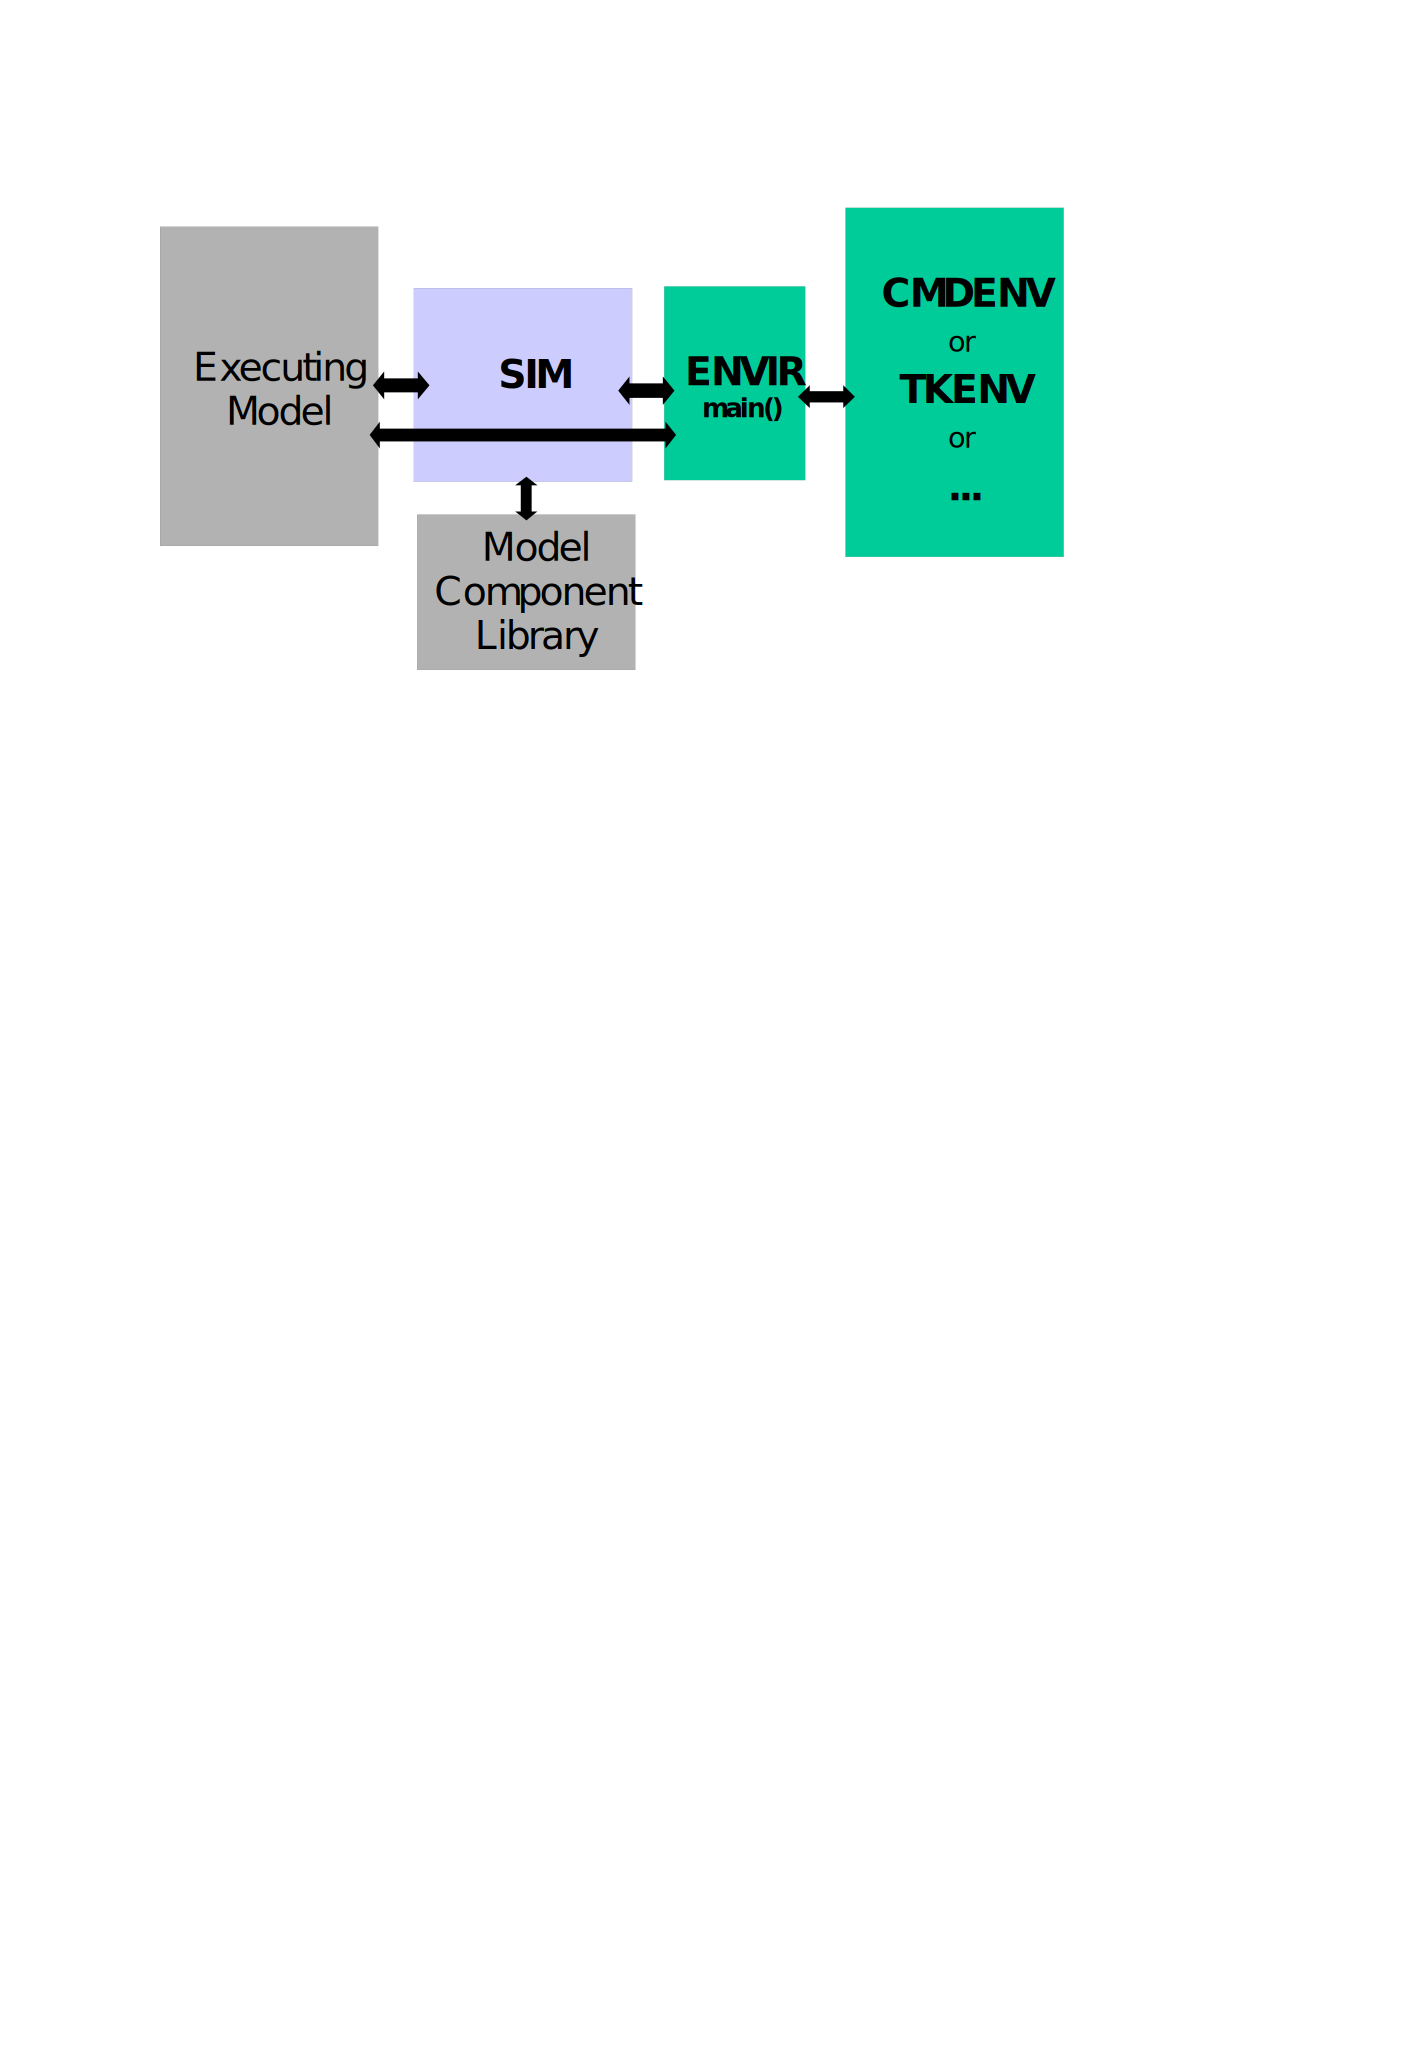
\includegraphics[width=4.757in, height=2.412in]{figures/usmanFig18}
    \caption{Architecture of {\opp} simulation programs}
  \end{center}
\end{figure}

The rectangles in the picture represent components:

\begin{itemize}
  \item{\textbf{Sim} is the simulation kernel and class
    library\index{simulation!kernel}. Sim exists as a library you link
    your simulation program with.
       \footnote{Use of dynamic (shared) libraries is also possible, but
       for simplicity we'll use the word \textit{linking} here.}
    }
  \item{\textbf{Envir} is another library which contains all code
    that is common to all user interfaces. \fname{main()} is also in Envir.
    Envir provides services like ini file handling for specific user interface
    implementations. Envir presents itself towards Sim and the executing model
    via the \ttt{ev} facade object, hiding all other user interface internals.
    Some aspects of Envir can be customized\index{customization} via plugin
    interfaces. Embedding {\opp} into applications\index{embedding} can
    be achieved implementing a new user interface in addition to Cmdenv and Tkev,
    or by replacing Envir with another implementation of \ttt{ev}
    (see sections \ref{sec:ch-opp-design:customization} and
    \ref{sec:ch-opp-design:embedding}.)}
  \item{\textbf{Cmdenv and Tkenv} are specific user interface
    implementations. A simulation is linked with
    either Cmdenv or Tkenv.}
  \item{The \textbf{Model Component Library} consists of simple module definitions and
    their C++ implementations, compound module types, channels, networks,
    message types and in general everything that belongs to models and
    has been linked into the simulation program. A simulation program is
    able to run any model that has all necessary components linked in.}
  \item{The \textbf{Executing Model} is the model that has been set up
    for simulation. It contains objects (modules, channels, etc.) that
    are all instances of components in the model component library.}
\end{itemize}

The arrows in the figure show how components interact with
each other:

\begin{itemize}
  \item{\textbf{Executing Model vs Sim}. The simulation kernel
    manages the future events and invokes modules in the executing model
    as events occur. The modules of the executing model are stored
    in the main object of Sim, \fvar{simulation} (of class \cclass{cSimulation}).
    In turn, the executing model calls functions in the
    simulation kernel and uses classes in the Sim library.}
  \item{\textbf{Sim vs Model Component Library}. The simulation kernel
    instantiates simple modules and other components when the simulation model
    is set up at the beginning of the simulation run. It also refers
    to the component library when dynamic module creation is used.
    The machinery for registering and looking up components in the model
    component library is implemented as part of Sim.}
  \item{\textbf{Executing Model vs Envir}. The \ttt{ev} object, logically
    part of Envir, is the facade of the user interface towards the executing model.
    The model uses \ttt{ev} to write debug logs (\ttt{ev<<}, \ttt{ev.printf()}).}
  \item{\textbf{Sim vs Envir}. Envir is in full command of what
    happens in the simulation program. Envir contains the \ttt{main()} function
    where execution begins. Envir determines which models should be set up
    for simulation, and instructs Sim to do so. Envir contains the main
    simulation loop (\textit{determine-next-event}, \textit{execute-event}
    sequence) and invokes the simulation kernel for the necessary
    functionality (event scheduling and event execution are implemented in Sim).
    Envir catches and handles errors and exceptions that occur
    in the simulation kernel or in the library
    classes during execution. Envir presents a single facade object (\ttt{ev})
    that represents the environment (user interface) toward Sim -- no Envir
    internals are visible to Sim or the executing model.
    During simulation model setup, Envir supplies parameter values for
    Sim when Sim asks for them. Sim writes output vectors via Envir,
    so one can redefine the output vector storing mechanism by changing Envir.
    Sim and its classes use Envir to print debug information.}
  \item{\textbf{Envir vs Tkenv and Cmdenv}. Envir defines \cclass{TOmnetApp}
    as a base class for user interfaces, and Tkenv and Cmdenv both subclass
    from \cclass{TOmnetApp}. The \ttt{main()} function provided as part of Envir
    determines the appropriate user interface class (subclassed from
    \cclass{TOmnetApp}), creates an instance and runs it -- whatever
    happens next (opening a GUI window or running as a command-line program)
    is decided in the \ttt{run()} method of the appropriate \cclass{TOmnetApp}
    subclass. Sim's or the model's calls on the \ttt{ev} object are
    simply forwarded to the \cclass{TOmnetApp} instance. Envir presents
    a framework and base functionality to Tkenv and Cmdenv via the methods of
     \cclass{TOmnetApp} and some other classes.)}
\end{itemize}


\section{Embedding {\opp}}
\label{sec:ch-opp-design:embedding}

This section discusses the issues of embedding the simulation kernel
or a simulation model into a larger application.

What you'll absolutely need for a simulation to run is the Sim library. You
probably do not want to keep the appearance of the simulation program, so
you do not want Cmdenv and Tkenv. You may or may not want to keep Envir.
You can keep Envir if its philosophy and the infrastructure it provides
(\ttt{omnetpp.ini}, certain command-line options etc.) fit into your
design. Then your application, the embedding program will take the place of
Cmdenv and Tkenv.

If Envir does not fit your needs (for example, you want the model
parameters to come from a database not from \ttt{omnetpp.ini}), then you
have to replace it. Your Envir replacement (the embedding application,
practically) must implement the \cclass{cEnvir} member functions from
\ttt{envir/cenvir.h}, but you have full control over the simulation.

Normally, code that sets up a network or builds the internals of a
compound module comes from compiled NED source.  You may not like the
restriction that your simulation program can only simulate networks
whose setup code is linked in. No problem; your program can contain
pieces of code similar to what is currently generated by nedc and then it can build
any network whose components (primarily the simple modules) are linked
in. Moreover, it is possible to write an integrated environment where
you can put together a network using a graphical editor and right
after that you can run it, without intervening NED compilation and
linkage.





\section{Sim: the simulation kernel and class library}

There is little to say about Sim here, since chapters
\ref{cha:simple-modules} and \ref{cha:the-simulation-library},
and part of chapter \ref{cha:messages} are all about
this topic. Classes covered in those chapters are documented
in more detail in the API Reference generated by Doxygen.
What we can do here is elaborating on some internals
that have not been covered in the general chapters.

The source code for the simulation kernel\index{simulation!kernel}
and class library reside in the \ttt{src/sim/} subdirectory.


\subsection{The global simulation object}

The global \ttt{simulation} object is an instance of \cclass{cSimulation}.
It stores the model, and encapsulates much of the functionality
of setting up and running a simulation model.

\ttt{simulation} has two basic roles:

\begin{itemize}
  \item{it stores modules of the executing model}
  \item{it holds the future event set (FES) object}
\end{itemize}



\subsection{The coroutine package}

The coroutine package is in fact made up of two coroutine
packages\index{coroutine}:

\begin{itemize}
  \item A portable coroutine package creates all coroutine stacks
     inside the main stack. It is based on Kofoed's solution\cite{Kofoed95}.
     It allocates stack by deep-deep recursions and then plays with
     \fname{setjmp()} and \fname{longjmp()} to switch from one to another.

  \item On Windows, the Fiber functions (\fname{CreateFiber()},
     \fname{SwitchToFiber()}, etc) are used, which are part of
     the standard Win32 API.
\end{itemize}

The coroutines are represented by the \cclass{cCoroutine}
class. \cclass{cSimpleModule} has \cclass{cCoroutine} as one a
base class.



\section{The Model Component Library}

All model components (simple module definitions and their C++
implementations, compound module types, channels, networks,
message types, etc.) that you compile and link into a simulation
program are registered in the Model Component Library.
Any model that has all its necessary components in the
component library of the simulation program can be run by that
simulation program.

If your simulation program is linked with Cmdenv or Tkenv,
you can have the contents of its component library printed,
using the -h switch.

\begin{verbatim}
% ./fddi -h

OMNeT++ Discrete Event Simulation  (C) 1992-2004 Andras Varga
...
Available networks:
  FDDI1
  NRing
  TUBw
  TUBs

Available modules:
  FDDI_MAC
  FDDI_MAC4Ring
  ...

Available channels:
  ...
End run of OMNeT++
\end{verbatim}

Information on components are kept on registration lists.
There are macros for registering components (that is, for adding
them to the registeration lists):
\ttt{\fmac{Define\_Module()}}, \ttt{\fmac{Define\_Module\_Like()}},
\ttt{\fmac{Define\_Network()}}, \ttt{\fmac{Define\_Function()}},
\fmac{Register\_Class()}, and a few others. For components defined
in NED files, the macro calls are generated by the NED compiler;
in other cases you have to write them in your C++ source.

Let us see the module registrations as an example. The

\begin{verbatim}
Define_Module(FIFO);
\end{verbatim}

macro expands to the following code:

\begin{verbatim}
static cModule *FIFO__create(const char *name, cModule *parentmod)
{
    return new FIFO(name, parentmod);
}

EXECUTE_ON_STARTUP( FIFO__mod,
    modtypes.instance()->add(
       new cModuleType("FIFO","FIFO",(ModuleCreateFunc)FIFO__create)
    );
)
\end{verbatim}

When the simulation program starts up, a new \cclass{cModuleType}
object will be added to the \ttt{modtypes} object, which holds the list
of available module types. The \cclass{cModuleType} object will act as a factory:
when its create() method is called it will produce a new module object
of class \ttt{FIFO} via the above static function \ttt{FIFO\_\_create}.

The \ttt{cModuleType} object also stores the name of the corresponding
NED module declaration. This makes it possible to add the gates and parameters
declared in NED to the module when it is created.

The machinery for managing the registration lists are part
of the Sim library. Registration lists are implemented
as global objects.

The registration lists are:

\begin{longtable}{|p{2cm}|p{4,3cm}|p{7.3cm}|}
\hline
%% ROW 1
\tabheadcol
\textbf{List variable}
&
\textbf{Macro/}\linebreak
\textbf{Objects on list}
&
\textbf{Function} \\\hline
%% ROW 2
\ttt{networks}
&
\ttt{\fmac{Define\_Network()}} \linebreak
\linebreak
\ttt{\cclass{cNetworkType}}
&
{\raggedright List of available networks\index{network!list of}.
A \cclass{cNetworkType} object holds a pointer to a function that can
build up the network.
\fmac{Define\_Network()} macros occur in the code generated by the NED
compiler.}\\\hline
% ROW 3
\ttt{modtypes}
&
\ttt{\fmac{Define\_Module()},} \linebreak
\ttt{\fmac{Define\_Module\_Like()},}  \linebreak
\linebreak
\ttt{\cclass{cModuleType}}
&
{\raggedright List of available module types.
A \cclass{cModuleType} object knows how to create a module of a specific
type. If it is compound, it holds a pointer to a function that can
build up the inside.
Usually, \fmac{Define\_Module()} macros for compound modules occur in
the code generated by the NED compiler; for simple modules,
the \fmac{Define\_Module()} lines are added by the user.}\\\hline
%% ROW 4
\ttt{classes}
&
\fmac{Register\_Class()} \linebreak
\linebreak
\ttt{cClassRegister}
&
{\raggedright List of available classes of which one can create
an instance.
A \cclass{cClassRegister} object has a ``factory method'' for creating an object
of a specific class. The list is used by the \fname{createOne()} function:
it can create an object of any class, given the class name as a string.
(E.g. the statement \ttt{ptr = createOne("cArray")} creates a \ttt{cArray} object.)
To enable a class to work with \ttt{createOne()}, one has to register it using the
\ttt{Register\_Class(classname)} macro}\\\hline
%% ROW 5
\ttt{functions}
&
\ttt{\fmac{Define\_Function()}} \linebreak
\linebreak
\ttt{\cclass{cFunctionType}}
&
{\raggedright List of functions taking \ttt{double}s and returning a \ttt{double}
(see type \ttt{MathFuncNoArg}...\ttt{MathFunc3Args}).
A \cclass{cFunctionType} object holds a pointer to the function and knows
how many arguments it takes.}\\\hline
%% ROW 6
\ttt{linktypes}
&
\fmac{Define\_Link()} \linebreak
\linebreak
%FIXME this is obsolete!!!!!!!!
\cclass{cLinkType}
&
{\raggedright List of link types.
A \cclass{cLinkType} object knows how to create \cclass{cPar} objects representing
the delay\index{channel!delay}, error\index{channel!error} and datarate\index{channel!datarate} attributes for a channel.
\fmac{Define\_Link()} macros occur in the code generated by the NED
compiler, one for each channel definition.} \\\hline
\end{longtable}





\section{Envir, Tkenv and Cmdenv}

The source code for the user interface of {\opp} resides in the
\texttt{src/envir/} directory (common part) and in the \texttt{src/cmdenv/},
\texttt{src/tkenv/} directories.

The classes in the user interface are \textit{not} derived from \cclass{cObject},
they are completely separated from the simulation kernel.



\subsection{The main() function}

The \fname{main()} function of {\opp} simply sets up the user
interface and runs it. Actual simulation is done in
\fname{cEnvir::run()} (see later).



\subsection{The cEnvir interface}

The \cclass{cEnvir} class has only one instance, a global object
called \fvar{ev}:

\begin{verbatim}
cEnvir ev;
\end{verbatim}

\cclass{cEnvir} basically a facade, its member functions
contain little code. \cclass{cEnvir} maintains a pointer to a
dynamically allocated simulation application object (derived from
\cclass{TOmnetApp}, see later) which does all actual work.


\cclass{cEnvir} member functions perform the following groups of tasks:
\begin{itemize}
  \item I/O for module activities; the actual implementation is different
    for each user interface (e.g. stdin/stdout for Cmdenv, windowing
    in Tkenv)
  \item cEnvir provides methods for the simulation kernel to
    access configuration information (for example, module parameter settings)
  \item cEnvir also provides methods that are called by simulation kernel to
    notify the user interface of certain events (an object was deleted;
    a module was created or deleted; a message was sent or delivered, etc.)
\end{itemize}


\subsection{Customizing Envir}
\label{sec:ch-opp-design:customization}

Certain aspects of Envir can be customized via plugin interfaces.
Plugin interfaces are presented in the form of C++ abstract classes
that you have to implement, register via the \fmac{Register\_Class()}
macro, and finally tell Envir to use them via \ttt{omnetpp.ini} entries.

The following plugin interfaces are supported:

\begin{itemize}
   \item{\cclass{cRNG}. Interface for the random number generator.}
   \item{\cclass{cScheduler}. The scheduler class. This plugin interface
     allows for implementing real-time, hardware-in-the-loop, distributed
     and distributed parallel simulation.}
   \item{\cclass{cConfiguration}. It defines a class
     from which all configuration will be obtained. In other words, it
     option lets you replace \ttt{omnetpp.ini} with some other implementation,
     e.g. database input.}
   \item{\cclass{cOutputScalarManager}. It handles recording the scalar output data,
     output via the cModule::recordScalar() family of functions.
     The default output scalar manager is \cclass{cFileOutputScalarManager},
     defined in the Envir library.}
   \item{\cclass{cOutputVectorManager}. It handles recording the output
     for \cclass{cOutVector} objects.
     The default output vector manager is \cclass{cFileOutputVectorManager},
     defined in the Envir library.}
   \item{\cclass{cSnapshotManager}. It provides an output stream to which
     snapshots are written (see section \ref{sec:ch-sim-lib:snapshots}).
     The default snapshot manager is \cclass{cFileSnapshotManager},
     defined in the Envir library.}
\end{itemize}

The above interfaces are documented in the API Reference.

The corresponding ini file entries that allow you to select your
plugin classes are \fpar{configuration-class}, \fpar{scheduler-class},
\fpar{rng-class}, \fpar{outputvectormanager-class},
\fpar{outputscalarmanager-class} and \fpar{snapshotmanager-class},
documented in section \ref{sec:ch-run-sim:general-section}.

\subsubsection{How plugin classes can access the configuration}

The configuration is available to plugin classes via the \fname{config()}
method of \cclass{cEnvir}, which returns a pointer to the configuration
object (\cclass{cConfiguration}). This enables plugin classes to have
their own config entries.

An example which reads the \ttt{parsim-debug} boolean entry from the
\ttt{[General]} section, with \ttt{true} as default:

\begin{verbatim}
bool debug = ev.config()->getAsBool("General", "parsim-debug", true);
\end{verbatim}


\subsubsection{Startup sequence for the configuration plugin}

For the configuration plugin, the startup sequence is the following
(see \ttt{cEnvir::setup()} in the source code):

\begin{enumerate}
  \item First, \ttt{omnetpp.ini} (or the ini file(s) specified via the "-f"
     command-line option) are read.
  \item Shared libraries in \ttt{[General]/load-libs} are loaded.
     (Also the ones specified with the "-l" command-line option.)
  \item \ttt{[General]/configuration-class} is examined, and if it is present,
     a configuration object of the given class is instantiated.
     The configuration object may read further entries from the
     ini file (e.g. database connect parameters, or XML file name).
  \item The original \ttt{omnetpp.ini} \cclass{cInifile} configuration
     object is deleted. No other settings are taken from it.
  \item \ttt{[General]/load-libs} from the new configuration object is
     processed.
  \item Then everything goes on as normally, using the new configuration
     object.
\end{enumerate}

%FIXME cScheduler usage


\subsection{Implementation of the user interface: simulation applications}

The base class for simulation application is \cclass{TOmnetApp}.
Specific user interfaces such as \cclass{TCmdenv},
\cclass{TOmnetTkApp} are derived from \cclass{TOmnetApp}.

\cclass{TOmnetApp}'s member functions are almost all virtual.
\begin{itemize}
  \item{Some of them implement the \cclass{cEnvir} functions
    (described in the previous section)}
  \item{Others implement the common part of all user interfaces (for
    example: reading options from the configuration files; making the
    options effective within the simulation kernel)}
  \item{The \fname{run()} function is pure virtual (it is different
    for each user interface).}
\end{itemize}

\cclass{TOmnetApp}'s data members:
\begin{itemize}
  \item{a pointer to the object holding configuration file contents
    (type \cclass{cInifile});}
  \item{the options and switches that can be set from the
    configuration file (these members begin with \ttt{opt\_})}
\end{itemize}

Simulation applications:
\begin{itemize}
  \item{add new configuration options}
  \item{provide a \fname{run()} function}
  \sloppy
  \item{implement functions left empty in \cclass{TOmnetApp} (like
    \fname{breakpointHit()}, \fname{objectDeleted()}).}
\end{itemize}


%
% section{Writing inspectors for TkEnv}
%
% TBD
%

%%% Local Variables:
%%% mode: latex
%%% TeX-master: "usman"
%%% End:

\cleardoublepage

%% Indexing continues here

\begin{appendix}

%%  \chapter{OPNET and {\opp}}
\label{cha:opnet-and-omnet}

\section{Comparison of OPNET and {\opp}}

OPNET$^{TM}$ (from MIL3 Inc.) is a state-of-the art commercial simulation 
program for the modeling of communication systems. OPNET is designed 
to enable full-detail modeling: every tool is given to implement 
nonstandard protocols or behaviour.


A quote from the OPNET brochure:


\begin{itemize}
\item{\textit{OPNET presents an advanced graphical user 
interface that supports multi-windowing, makes use of menus and 
icons, and runs under X Windows. Supported platforms include 
popular engineering workstations from SUN, DEC, HP and Silicon 
Graphics. (Windows NT version also exists.)}}
\item{\textit{Graphical object-oriented editors for defining topologies 
and architectures directly parallel actual systems, allowing 
an intuitive mapping between a system and its model. OPNET's 
hierarchical approach simplifies the specification and representation 
of large and complex systems.}}
\item{\textit{The process editor provides a powerful and flexible 
language to design models of protocols, resources, applications, 
algorithms, queuing policies, and other processes. Specification 
is performed in the Proto-C language, which combines a graphical 
state-transition diagram approach with a library of more than 
300 communication- and simulation-specific functions. The full 
generality and power of the C language is also available.}}
\item{\textit{OPNET simulations generate user-selected performance 
and behavioral data. Simulation results can be plotted as time 
series graphs, scatter plots, histograms, and probability functions. 
Standard statistics and confidence intervals are easily generated 
and additional insight can be obtained by applying mathematical 
operators to the collected data. }}
\item{\textit{OPNET provides an advanced animation capability for 
visualising simulation events. Both automatic and user-customised 
animations can be displayed interactively during or after a simulation. 
Animations can depict messages flowing between objects, control 
flow in a process, paths of mobile nodes, and dynamic values 
such as queue size or resource status. }}
\item{\textit{OPNET provides open system features including: interfaces 
to standard languages; the ability to take advantage of third-party 
libraries; an application program interface; access to databases 
and data files such as those generated by network analysers; 
and PostScript and TIFF export for desktop publishing. OPNET 
users are guided by a comprehensive documentation set and are 
backed by outstanding technical support.}}
\end{itemize}

OPNET is very well designed and built commercial simulation software. 
The author of {\opp} has worked for the Hungarian distributor 
of OPNET for over three years and he has gained significant experience 
with the software. He has taken part in several computer network 
simulation projects for major Hungarian companies and also delivered 
OPNET training. He has also written simulation models for a VSAT 
system in OPNET. \\
Following is a comparison of the features that concern general-purpose 
computer systems simulation (and are not specific to computer 
network simulation) and that are present both in {\opp} and 
OPNET.


\textbf{Model hierarchy levels}
\begin{longtable}{|p{7cm}|p{7cm}|}
  \hline
%% ROW 1
  \tabheadcol
  \textbf{OPNET} & \textbf{{\opp}}\\\hline
%% ROW 2
  {\raggedright network level (subnetwork nesting possible)\hfill} \linebreak
  {\raggedright node level (no nesting)\hfill} \linebreak
  process level (no nesting)
  & 
  arbitrary levels of submodule nesting \\\hline
\end{longtable}



\textbf{Topology description method}


OPNET provides two tools for defining module topology: graphical 
editors to design network and node level models, and EMA (External 
Model Access), an API for building model files from C programs. 
These tools correspond to {\opp}'s tools in the following way:


\begin{longtable}{|p{4.5cm}|p{4.5cm}|p{4.5cm}|}
\hline
%% ROW 1
\tabheadcol
 & \textbf{OPNET} & \textbf{{\opp}}\\\hline
%% ROW 2
\textbf{Graphical} & graphical editor within the IDE & graphical editor: GNED \\\hline
%% ROW 3
\textbf{High-level} & - & NED language\\\hline
%% ROW 4
\textbf{Low-level} & EMA & C++ output of NED compilation\\\hline
\end{longtable}



There is no high-level textual model description in OPNET (like 
NED is in {\opp}). This means that one has either to use the 
graphical editor or write lengthy C code using the EMA API.


The OPNET graphical model editor can only create fixed (non-parameterized) 
topologies.


There's a significant difference between how EMA and {\opp}'s 
NED are used. OPNET's EMA generates model files. EMA applications 
are standalone programs: one writes the EMA C code, compiles 
and runs it, and the EMA executable will generate a model file 
that can be read into the graphical editor or loaded by simulation 
programs. EMA cannot be used from within a simulation program. 
In contrast, the compiled NED code of {\opp} becomes part of 
the simulation program and it builds the model without having 
to run external programs; this means that you can have a single 
simulation executable that can be used to perform simulation 
studies on networks with different topologies.


\textbf{Module parameters}

\begin{longtable}{|p{4.5cm}|p{4.5cm}|p{4.5cm}|}
\hline
% ROW 1
\tabheadcol
& \textbf{OPNET} & \textbf{{\opp}}\\\hline
% ROW 2
\textbf{Expressions} & no expressions are allowed: only literals or exact copy of another 
parameter & arbitrary expressions using other parameters \\\hline
% ROW 3
\textbf{Parameter passing} & by value & parameters can be passed by value or by reference, and be changed during simulation\\\hline
% ROW 4
\textbf{Usage} & by process models only & by process models; also to define flexible topologies \\\hline
\end{longtable}



In OPNET, module parameter values can be passed only ''as 
is''.


\textbf{Packet streams or gates\\
}

\begin{longtable}{|p{4.5cm}|p{4.5cm}|p{4.5cm}|}
\hline
%% ROW 1
\tabheadcol
& 
\textbf{OPNET} & 
\textbf{{\opp}}\\\hline
%% ROW 2
\textbf{Identification} & 
Packet streams are numbered from 0; no names can be assigned. & 
{\raggedright Gates are identified by names. Gate vectors are supported.\\
In the code, gates can be referenced by ID for greater speed.}\\\hline
%% ROW 3
\textbf{Directionality} & 
Packet streams are uni-directional. & 
Gates are uni-directional.\\\hline
\end{longtable}


\textbf{Flexible topologies}

\begin{longtable}{|p{7cm}|p{7cm}|}
\hline
%% ROW 1
\tabheadcol
\textbf{OPNET} & 
\textbf{{\opp}}\\\hline
%% ROW 2
not really supported\footnote{If really necessary, it can be done through C programming (writing 
EMA code) and running external program to create a separate model  file for each case.}
& 
in the NED file, parameters can define submodule types, count 
of submodules, gates and describe connections \\\hline
\end{longtable}





\textbf{Tracing, animation and interactive simulation}

\begin{longtable}{|p{4.5cm}|p{4.5cm}|p{4.5cm}|}
\hline
%% ROW 1
\tabheadcol
 & \textbf{OPNET} & \textbf{{\opp}}\\\hline
%% ROW 2
\textbf{Tracing and debugging}
& 
powerful command line debugger (ODB)
& 
separate window for each module's output, single-steps, run 
until, inspectors, snapshot, etc. (Tkenv) \\\hline
%% ROW 3
\textbf{Animation}
& 
{\raggedright mostly used in record/ playback mode;\hfill} \linebreak
animation spec. must be given in advance (via anim. probes)
& 
interactive execution with message-flow animation, statistics 
animation etc. (Tkenv) \\\hline
%% ROW 4
\textbf{Interactive simulation}
& 
not supported
& 
strongly supported via object inspectors and watches. (Tkenv) \\\hline
\end{longtable}


\textbf{Random numbers}

\begin{longtable}{|p{4.5cm}|p{4.5cm}|p{4.5cm}|}
\hline
%% ROW 1
\tabheadcol
& \textbf{OPNET} & \textbf{{\opp}}\\\hline
%% ROW 2
\textbf{Distributions provided}
& 
many built-in distributions (through algorithms)
& 
four built-in distributions, as C functions \\\hline
%% ROW 3
\textbf{Additional distributions}
& 
through histograms
& 
as C functions (algorithms); or through histograms \\\hline
%% ROW 4
\textbf{Random number generation}
& 
one random number generator, no support for seed selection
& 
{\raggedright several independent random number generators;\\
tool to support selecting good seed values} \\\hline
\end{longtable}



OPNET has many built-in distributions implemented with algorithms 
(C functions). Additional distributions are supported as histograms. 
There is only one common source of random numbers. OPNET has 
no aid for selecting seed values that produce long non-overlapping 
random number sequences.


{\opp}, only four basic distributions are provided. They are 
implemented as C functions. Additional distributions can be added 
by the user, and they are treated exactly in the same way as 
built-in ones. Defining and using distributions in histogram 
form is also supported. {\opp} provides several random number 
generators, and also a tool for selecting good seed values.


\textbf{Process description method}

\begin{longtable}{|p{4.5cm}|p{4.5cm}|p{4.5cm}|}
\hline
%% ROW 1
\tabheadcol
& \textbf{OPNET} & \textbf{{\opp}}\\\hline
% ROW 2
\textbf{Method}
&
finite state machine (graphical spec. only)
& 
both process-style (coroutine-based) and finite state machine 
(textual spec. only)\\\hline
\end{longtable}



\textbf{Direct (non-scheduled) process interaction}

\begin{longtable}{|p{4.5cm}|p{4.5cm}|p{4.5cm}|}
\hline
%% ROW 1
\tabheadcol
& \textbf{OPNET} & \textbf{{\opp}}\\\hline
%% ROW 2
\textbf{Method} & ''forced interrupt'' & member function call of other module\\\hline
\end{longtable}



\textbf{Dynamic module creation}

\begin{longtable}{|p{4.5cm}|p{4.5cm}|p{4.5cm}|}
\hline
% ROW 1
\tabheadcol
& \textbf{OPNET} & \textbf{{\opp}}\\\hline
% ROW 2
\textbf{What can be created}
&
only processes within an existing module
& 
{\raggedright simple\index{module!simple} modules;\\
connections;\\
compound\index{module!compound} modules with arbitrarily complex, parameterized topologies}\\\hline
\end{longtable}



\textbf{Object-oriented concepts}

\begin{longtable}{|p{4.5cm}|p{4.5cm}|p{4.5cm}|}
\hline
% ROW 1
\tabheadcol
& \textbf{OPNET} & \textbf{{\opp}}\\\hline
% ROW 2
\textbf{Language} & C & C++\\\hline
% ROW 3
\textbf{Objects}
& 
{\raggedright C API functions operating on object-like data structures;\\
no support for inheritance\footnote{The graphical user interface of OPNET (from version 3.0) contains an ''inheritance mechanism'' for models. This is no real inheritance in the object-oriented sense because it just means that parameter values can be changed or fixed down, parameters renamed, merged etc. There is no mention about changing the behaviour of a module (that is, anything like C++'s virtual functions).}, polymorphism or the like}
& 
{\raggedright full flexibility of C++: inheritance, polymorphism etc;\\
built-in object-oriented mechanisms}\\\hline
\end{longtable}


\textbf{Statistics collection and run-time analysis}

\begin{longtable}{|p{7cm}|p{7cm}|}
\hline
%% ROW 1
\tabheadcol
\textbf{OPNET} & \textbf{{\opp}}\\\hline
%% ROW 2
{\raggedright writing observations to output file; ''probes'' 
to select statistics to be collected;\\
only off-line analysis (analysis of output files) is supported}
& 
{\raggedright writing observations to output files (roughly equivalent to 
OPNET's solution);\\
run-time processing: basic measures (mean etc); distribution 
estimation with histograms; quantiles ($P^{2}$ algorithm);\\
support for detecting the end of the transient period and sufficient 
result accuracy}\\\hline
\end{longtable}



\textbf{Parallel execution}

\begin{longtable}{|p{7cm}|p{7cm}|}
\hline
%% ROW 1
\tabheadcol
\textbf{OPNET} & \textbf{{\opp}}\\\hline
%% ROW 2
 not supported & supported by PVM and MPI; arbitrary synchronization can be used\\\hline
\end{longtable}



\textbf{Openness}

\begin{longtable}{|p{4.5cm}|p{4.5cm}|p{4.5cm}|}
\hline
%% ROW 1
\tabheadcol
 & \textbf{OPNET} & \textbf{{\opp}}\\\hline
%% ROW 2
\textbf{Input file formats}
&
{\raggedright binary model files\footnote{Can be read and analyzed by EMA programs.};\\
textual parameter files}
& 
text files \\\hline
%% ROW 3
\textbf{Output file formats}
& 
binary files\footnote{Can be exported to text files from the main OPNET program.}
& 
text files\\\hline
%% ROW 4
\textbf{Availability of source}
& 
not available (only the source of the shipped models is available)
& 
available\\\hline
%% ROW 5
\textbf{Embedding simulations into other software product}
& 
not supported and also not possible (the \fname{main()} function cannot 
be supplied by the user etc.)
& 
{\raggedright supported.\\
Embedding application becomes a new ''user interface'' 
based on Envir (1); or embedding application replaces Envir (2).}\\\hline
\end{longtable}










\section{Quick reference for OPNET users}

This section is intended to help OPNET users learn {\opp} faster.

\begin{longtable}{|p{6cm}|p{8cm}|}
\hline
%% ROW 1
\tabheadcol
\textbf{OPNET} & \textbf{{\opp}}\\\hline
%% ROW 2
network, subnetwork, node & Compound modules\\\hline
%% ROW 3
module, process & An {\opp} simple\index{module!simple} module corresponds to an OPNET module with 
its process.\\\hline
%% ROW 4
interrupts, invocations, states
& 
{\raggedright When using \fname{handleMessage()}: interrupt = event, invocation = call 
to \fname{handleMessage()}, state = FSM state or the value of the state 
vars stored in the class\hfill} \linebreak
{\raggedright When using modules with \fname{activity()}, this means a little different 
way of thinking from OPNET's. In {\opp}, you write a simple\index{module!simple}
module as you would write an operating system process or a thread, 
thus there's no need to distinguish 'states' or speak about 'invocations'. 
Within the simulation kernel, an 'invocation' corresponds to 
a \ttt{transferTo(\textit{module})} call.\hfill} \linebreak
{\raggedright An {\opp} module accepts messages (and simulation time advances) 
within \ttt{receive\dots (\dots )} calls; \fname{wait()} is just a \fname{scheduleAt()} followed 
by a \fname{receive()}.\hfill} \linebreak
An OPNET interrupt is the event being processed. In this sense, 
{\opp} messages returned by \fname{receive()} correspond to OPNET interrupts.\\\hline
%% ROW 5
endsim interrupt
& 
The \fname{finish()} virtual member functions of the simple\index{module!simple} modules are 
called at the end of the simulation run. You can redefine \fname{finish()}
to write statistics etc. \\\hline
%% ROW 6
\multicolumn{2}{c}{}\\\hline
%% ROW 7
\ttt{op\_ima\_obj\_attr\_get(\dots )}
& 
{\raggedright \ttt{foo = par(''foo'');}\hfill} \linebreak
\ttt{foo = module-\texttt{>}par(''foo'');}\\\hline
%% ROW 8
\ttt{op\_ima\_sim\_attr\_get(\dots )}
& 
{\raggedright There are no simulation attributes. You can use the parameters 
of the top-level module instead:\hfill} \linebreak
\ttt{foo = simulation.systemModule()-\texttt{>}par(''foo'');}\\\hline
%% ROW 9
\multicolumn{2}{c}{}\\\hline
% ROW 10
{\raggedright \ttt{op\_prg\_odb\_print\_minor(\dots )} \hfill} \linebreak
\ttt{op\_prg\_odb\_print\_major(\dots )}
& 
{\raggedright \ttt{ev << ''hello!'' << endl;}\hfill} \linebreak
\ttt{ev.printf(\dots );}\\\hline
%% ROW 11
\ttt{op\_sim\_end(\dots )}
& 
\ttt{simulation.error(''Your fault! error \%d'',ec);}\\\hline
%% ROW 12
\multicolumn{2}{c}{} \\\hline
%% ROW 13
\ttt{op\_subq\_....()}
& 
{\raggedright Create a queue object and then manipulate it with its member 
  functions.\hfill}
\begin{Verbatim}
cQueue queue;
queue.insert( msg );
if (!queue.empty())
  msg = queue.pop();
\end{Verbatim}
\\\hline

%% ROW 14
{\raggedright \ttt{List}\hfill} \linebreak
\ttt{op\_prg\_list\_...()}
& 
\begin{Verbatim}
cLinkedList list;
list.insert( ptr );
if (!list.empty())
ptr = list.pop();
\end{Verbatim}
\\\hline

%% ROW 15
\multicolumn{2}{c}{}\\\hline

%% ROW 16
{\raggedright \ttt{Topology}\hfill} \linebreak
\ttt{op\_rte\_...()}
& 
The \cclass{cTopology} class offers similar functionality, and you can 
expect greater speed than with OPNET's routing functions. \\\hline

%% ROW 17
\multicolumn{2}{c}{}\\\hline

%% ROW 18
\begin{Verbatim}
Packet
op_pk_create(... )
op_pk_destroy( )
\end{Verbatim}
& 
{\raggedright Use the \cclass{cMessage} class.\hfill}
\begin{Verbatim}
cMessage *msg = new cMessage;
delete msg;
\end{Verbatim}
\\\hline

%% ROW 19
{\raggedright packet fields\hfill}
\begin{Verbatim}
op_pk_nfd_set(... )
op_pk_nfd_get_(... )
op_pk_fd_set(... )
op_pk_fd_get(... )
\end{Verbatim}
& 
{\raggedright Message parameters. A parameter has both name and index.\hfill} \linebreak
\begin{Verbatim}
msg->par("foo") = foo;
msg->addPar("new-foo") = foo;
int foo = msg->par("foo");

int fooindex =
  msg->parList().find("foo");
msg->par(fooindex) = foo;
\end{Verbatim}
\\\hline

%% ROW 20
packet field modeled size
& 
{\raggedright Message parameters do not have associated modelled bit sizes. 
  Message length can be used instead.\hfill} \linebreak
\begin{Verbatim}
msg->addPar("dest_addr") = dest_addr;
msg->addLength( 32 );
\end{Verbatim}
\\\hline

%% ROW 21
packet formats
&
There are no explicit packet formats in {\opp}. However, you 
can write function to create messages with specific fields and 
length:
\begin{Verbatim}
cMessage *createEthernetFrame()
{
  cMessage *msg = new cMessage; 
  msg->setKind(PACKET);
  msg->addPar("source");
  msg->addPar("destination");
  msg->addPar("protocol");
  msg->setLength( 8*16 );
  return msg;
}
\end{Verbatim}
\\\hline

%% ROW 22
packet encapsulation
& 
{\raggedright As in OPNET, message parameters can be assigned object pointers, 
thus also message pointers.\hfill}  \linebreak
However, there is also direct support encapsulation:
\begin{Verbatim}
msg->encapsulate(innermsg)
innermsg = msg->encapsulatedMsg();
innermsg = msg->decapsulate();
\end{Verbatim}
\\\hline

%% ROW 23
ICI
& 
{\raggedright ICIs are also represented by cMessage objects, naturally with 
zero length.\hfill}  \linebreak
If it is important to distinguish between packets and ICIs, you 
can use the message kind field:
\begin{Verbatim}
#define PACKET 0
#define ICI 1

cMessage *pk = new cMessage;
pk->setKind(PACKET);

cMessage *ici = new cMessage;
ici->setKind(ICI);
\end{Verbatim}
\\\hline

%% ROW 24
ICI formats & See packet formats.\\\hline
%% ROW 25
ICI attributes & See packet fields.\\\hline
%% ROW 26
packet and ICI in the same interrupt
& 
You can use encapsulation. At the sender side:
\begin{Verbatim}
cMessage *ici, *pk;
ici->encapsulate(pk);
send(ici,"out-gate");
\end{Verbatim}
The receiver side:
\begin{Verbatim}
ici = receive();
pk = ici->decapsulate();
\end{Verbatim}
\\\hline

%% ROW 27
\multicolumn{2}{c}{}\\\hline
%% ROW 28
\ttt{op\_pk\_send(\dots )}
& 
\begin{Verbatim}
send( msg, "out-gate");
send( msg, "gate-vector'', index);
send( msg, gate_id );
\end{Verbatim}
\\\hline

%% ROW 29
\ttt{op\_pk\_send\_delayed(\dots )} & \ttt{sendDelayed(\dots )}\\\hline
%% ROW 30
\ttt{op\_pk\_deliver(\dots )} & \ttt{sendDirect(\dots )}\\\hline

%% ROW 31
\multicolumn{2}{c}{}\\\hline

%% ROW 32
\ttt{op\_pk\_schedule\_self(\dots )} & \ttt{scheduleAt( simTime()+timeout, msg );}\\\hline
%% ROW 33
\ttt{op\_ev\_cancel(\dots )} & \ttt{cancelEvent( msg );}\\\hline

%% ROW 34
\multicolumn{2}{c}{}\\\hline

%% ROW 35
\ttt{op\_dist\_load(\dots ) \linebreak
  op\_dist\_outcome(\dots )}
& 
To generate random numbers from analytical distributions, use:
\begin{Verbatim}
uniform(... )
intuniform(... )
exponential(... )
normal(... )
truncnormal(... )
\end{Verbatim}

For custom distributions you can use the histogram classes. Histograms 
can load distribution data from file.
\begin{Verbatim}
cDoubleHistogram hist;
FILE *f = fopen("distribution.dat");
hist.loadFromFile( f );
fclose(f); 

double rnd = hist.random();
\end{Verbatim}
\\\hline

%% ROW 36
\multicolumn{2}{c}{}\\\hline

%% ROW 37
output vectors
& 
The \cclass{cOutVector} class can be used.
\begin{Verbatim}
cOutVector eed("End-to-end delay");

double d = msg->creationTime()
             - simTime();
eed.record( d );
\end{Verbatim}
\\\hline

%% ROW 38
output scalars
& 
Output scalar file exists. You can write into it with \ttt{recordScalar()}:
\begin{Verbatim}
recordScalar("average delay",
             avg_delay);
\end{Verbatim}
\\\hline

%% ROW 39
\multicolumn{2}{c}{}\\\hline

%% ROW 40
\ttt{op\_topo\_parent()} & \ttt{cModule *parent = parentModule();}\\\hline
%% ROW 41
\ttt{op\_topo\_child\_\dots (\dots )} & \ttt{cSubModuleIterator}\\\hline

%% ROW 42
\multicolumn{2}{c}{}\\\hline

%% ROW 43
\ttt{op\_topo\_..\_assoc\_(\dots )}
& 
\begin{Verbatim}
gate(i)/gate(name),
gate->toGate()/fromGate()
gate->destinationGate()/sourceGate()
gate->ownerModule()
\end{Verbatim}
\\\hline

%% ROW 44
\multicolumn{2}{c}{}\\\hline

%% ROW 45
\ttt{op\_pro\_create(\dots )}
& 
See dynamic module creation. Note that this is a more powerful 
tool than OPNET's dynamic processes in that you can also create 
compound modules. \\\hline

%% ROW 46
Prohandle
& 
Module ID. Given the module pointer, you can obtain module ID 
by
\begin{Verbatim}
int id = mod->id();
\end{Verbatim}

And you can obtain module pointer from the ID:
\begin{Verbatim}
cModule *mod = simulation.module(id);
\end{Verbatim}
An invalid ID is negative. \\\hline

%% ROW 47
\ttt{op\_pro\_invoke(\dots )}
& 
Dynamically created modules do not need to be invoked, they 
live their own life. To dispatch messages to them, you can use \ttt{sendDirect(\dots )}\\\hline

%% ROW 48
\begin{Verbatim}
op_pro_destroy(... )
op_pro_destroy( self )
\end{Verbatim}
& 
\begin{Verbatim}
deleteModule( module );
deleteModule();
\end{Verbatim}
\\\hline

%% ROW 49
module memory, parent-to-child memory, argument memory to dynamic processes
& 
{\raggedright Parent module can set pointers (void* data members) in the dynamically 
created module object any time, thus also right after creating 
it ( parent-to-child memory), right before sending a packet to it 
( argument memory), and the pointer can refer to memory managed 
by the parent module ( module memory).\hfill}  \linebreak
An example for argument memory. Suppose the child module class 
has a public data member named argmem:
\begin{Verbatim}
class ChildModule :
        public cSimpleModule {
  ...
  public
  void *argmem;
  ...
};
\end{Verbatim}

The parent module code would be:
\begin{Verbatim}
childmod->argmem = argument_memory_ptr;
sendDirect( msg, childmod, 0.0, "in" );
\end{Verbatim}
Child module code would be:
\begin{Verbatim}
msg = receive();
argument_memory_ptr = argmem;
\end{Verbatim}
\\\hline

%% ROW 50
\ttt{op\_pro\_valid(\dots )}
& 
Given the module id:
\begin{Verbatim}
int valid = (id>=0) &&
            simulation.exist(id);
\end{Verbatim}
\\\hline

%% ROW 51
\multicolumn{2}{c}{}\\\hline

%% ROW 52
Environment files
& 
Configuration files. Default is \ttt{omnetpp.ini}. Multiple ini files 
and ini file inclusion are also supported.\\\hline

%% ROW 53
Process Editor & Your favourite text editor. Or \textit{vi} :-).\\\hline

%% ROW 54
Network Editor, Node Editor
& 
{\raggedright Any editor to write NED files.\hfill} \linebreak
GNED. Not very sophisticated yet though. \\\hline

%% ROW 55
Simulation Tool & 
{\raggedright Use the \ttt{[Run 1]}, \ttt{[Run 2]} etc. sections
in \ttt{omnetpp.ini} do describe several runs with different
parameters.\hfill} \linebreak
To create loops on different variables, you can use a shell script 
that creates a short ini file with the variable parameters, and 
include that file in \ttt{omnetpp.ini}. \\\hline

%% ROW 56
probes, Probe Editor & 
From the ini file, you can turn on/off \cclass{cOutVector} objects individually 
as well as assign result collection interval to them. \\\hline

%% ROW 57
Analysis Tool &  Plove \\\hline

%% ROW 58
EMA & 
{\raggedright Where you would normally use EMA, {\opp} NED files with parameterized 
topology are often enough.\hfill} \linebreak
{\raggedright Otherwise, you have two choices:\hfill} \linebreak
{\raggedright a) write a program to generate NED files. Text-processing languages 
like \fprog{perl} and \fprog{awk} are great tools for that.\hfill} \linebreak
b) write the network-building code in C++. You can look at the 
output of nedc for some idea how to do it.\\\hline
\end{longtable}



%%% Local Variables: 
%%% mode: latex
%%% TeX-master: "usman"
%%% End: 

%%  \cleardoublepage

%%  \chapter{PARSEC and {\opp}}
\label{cha:parsec-and-omnet}


\section{What is PARSEC?}

PARSEC\index{PARSEC} is a very successful simulation language, with
strong support for parallel simulation. PARSEC bears some similarity
to {\opp} in that it is also based on threads and coroutines. The
language and the software has been developed at the Parallel Computing
Laboratory of the University of California at Los Angeles (UCLA),
under the leadership of Prof. Rajive Bagrodia. PARSEC has been used in
a number of simulation projects, for example in simulation of mobile
radio networks in a military environment.


It is best to quote the PARSEC User Manual, Release 1.1 (August
1998):


\textit{PARSEC (for PARallel Simulation Environment for Complex
  programs) is a C-based discrete event simulation language. It adopts
  the process interaction approach to discrete event simulation. An
  object (also referred to as a physical process) or a set of objects
  in the physical system is represented by a logical process} [a
thread -- roughly equivalent to an {\opp} simple\index{module!simple} module
--Andras]\textit{. Interactions among physical processes (events) are
  modeled by timestamped message exchanges among the corresponding
  logical  processes.\\
  One of the important distinguishing features of PARSEC is its
  ability to execute a discrete-event simulation model using several
  different asynchronous parallel simulation protocols on a variety of
  parallel architectures. [...] Thus, with few modifications, a PARSEC
  program may be executed using the traditional sequential (Global
  Event List) simulation protocol or one of many parallel
  [...] protocols.\\
  In addition, PARSEC provides powerful message receiving constructs
  that result in shorter and more natural simulation programs.
  [...]\\
  The PARSEC language has been derived from the Maisie language, but
  with several improvements, both in the syntax of the language
  and in its execution environment.}

The PARSEC web site is at \href{http://pcl.cs.ucla.edu/}{http://pcl.cs.ucla.edu/}.


PARSEC is \textbf{\textit{not}} open source. It seems that the source code
is only available to research collaborators.





\section{What is inside the PARSEC package?}

When you download and install the PARSEC distribution, basically
you find:
\begin{itemize}
\item{pcc (the PARSEC compiler), and}
\item{2 variants of the PARSEC runtime library}
\end{itemize}


This shows that PARSEC is strictly a simulation (and parallel
programming) language which is restricted to the area of entities,
messages, and the tasks centered around message sending and receiving.
It is difficult to compare to {\opp} which is more of a complete
simulation environment. (The {\opp} simulation library alone
covers a much wider range of functionality than PARSEC as a whole.)


The primary strength of PARSEC is its parallel simulation support.
The manual only describes conservative PDES, but optimistic algorithms
are also supported. However, the distribution of Parallel PARSEC
is limited to research collaborators (personal communication
from Richard A. Meyer, Nov. 2001).





\section{PARSEC vs. the {\opp} simulation kernel}

This section gives a brief overview of PARSEC, with special attention
to the differences compared to {\opp}.

PARSEC is compared against the core functionality of the {\opp}
simulation kernel, that is, message sending/receiving and the
coroutines (\fname{activity()}). Other parts of the {\opp} simulation
kernel (e.g. statistics classes) and other parts of the {\opp}
package have no equivalent in PARSEC.


\textbf{Sample PARSEC code}


The PARSEC is a programming language based on C (\textit{not} C++!).
PARSEC programs, in addition to normal C code, contain special
syntactic constructs, so they do not compile as C. One has to
invoke the PARSEC compiler (\ttt{pcc}) on the source code in order
to translate it into C code that uses the PARSEC runtime library.


The main advantage of this solution is that the PARSEC language
is clean and really elegant.


Let us see a bit of PARSEC code:

\begin{verbatim}
#include <stdio.h>
...

message job {
   int id;
   int count;
};

message add_to_your_sorc {
   ename id;
};
...

entity driver(int argc, char **argv) {
...
}
\end{verbatim}

\textbf{Entities and messages}


In the above PARSEC code fragment, two constructs stand out at
once: \ttt{message} and \ttt{entity}.

The \ttt{message} constructs define message types, and they are translated
to C structs by pcc.


Entities correspond to {\opp}'s simple\index{module!simple} modules.
(PARSEC has no equivalent of {\opp}'s compound
modules.) The body of the entity contains the algorithm. Entities are
implemented with coroutines or threads much like {\opp}'s
\fname{activity()}-based simple\index{module!simple} modules; the
entity body is equivalent to the \fname{activity()} function.  (PARSEC
has no equivalent of \fname{handleMessage()}-based
simple\index{module!simple} modules.)


\ttt{ename} is a data type that holds entity references.


\textbf{Problems with splitting up the entity body}


During programming, the code of an entity may become so large
that it is no longer feasible to keep it within a single function
body. In {\opp} you can solve the problem by distributing the
simple\index{module!simple} module class's \fname{activity()} code into new member functions
which are called from \fname{activity()}, and moving the some local variables
of \fname{activity()} into the module class so that they can also be
accessed by the new member functions.

The above approach doesn't work in PARSEC, because PARSEC is
C-based and entities are not C++ classes. Of course one may call
ordinary C functions from the entity body, but the necessary
parameters must be passed in the argument list (or as pointers
to data structures).

Another solution in PARSEC is to use a construct called \textit{friend} \textit{functions}
(not to be confused with C++ friend functions). PARSEC's friend
functions may access the local variables of the entity (quite
strange in C, but much like an inner procedure in Pascal...).
However, the PARSEC documentation does not recommend using friend
functions (they are slow); it says they are provided for Maisie
compatibility.


\textbf{The driver entity}


The driver entity is special; in a way it is similar to the C \fname{main()}
function. PARSEC starts the simulation by creating and running
a driver entity. The main task of the driver is to create all
other entities in the simulation and provide them with information
they need (parameter values, etc). The latter is done by sending
out messages with the necessary parameters to all entities that
need it.


PARSEC does not have a high-level topology description language
like NED in {\opp}; instead, the driver entity is hand-coded
most of the time. (There was no mention of tools that could generate
the driver entity based on some higher-level description.).


{\opp} compound modules have no equivalent in PARSEC. All entities are
at the same level, there's no way to express hierarchy.


PARSEC has no notion of module gates, and there are no connections
(in the {\opp} sense) among the entities. This means that when
sending messages, the receiving entity must be explicitly named.
Since the program contains no explicit topology information,
an entity initially has no information about its communication
partners (it knows no enames except its own). The usual practice
is that the driver entity sends the necessary enames in an initialization
message to each entity. (For illustration, see the add\_to\_your\_sorc
message type from the above code fragment. The message name itself
is quite descriptive.)

The consequence of the lack of compound modules and module gates is
that it is a complicated and tricky task to set up networks with but
the most trivial topology. It is also very difficult to write reusable
simulation components without well-defined interfaces and structuring
(compound modules).


\textbf{C++ syntax not allowed}


It is not possible to use \textit{any} C++ constructs in PARSEC programs.
This means it is also impossible to use any C++ class libraries
in PARSEC programs; only C libraries can be used.

This limitation comes from pcc itself: the parser inside pcc
is written for C, and as such, it cannot parse C++ syntax. It
is irrelevant whether you use a C or C++ compiler to compile
pcc's output. One exception is that pcc accepts //-style comments.


\textbf{Message sending}


Messages can be sent to other entities with the \textit{send} construct:

\begin{Verbatim}[commandchars=\\\{\}]
\textbf{send} \textit{message} \textbf{to} \textit{dest-entity} \textbf{after} \textit{delay};
\end{Verbatim}

For example, creating a new message of type Request with the
parameters 10 and self (the current entity) and sending it to entity2
entity after a delay looks like this:

\begin{Verbatim}[commandchars=\\\{\}]
\textbf{send} Request\{10,\textbf{self}\} \textbf{to} entity2 \textbf{after} 5;
\end{Verbatim}

This PARSEC construct is totally equivalent in functionality
to {\opp}'s sendDirect( \textit{message}, \textit{delay}, \textit{dest}-\textit{module} [,\textit{dest}-\textit{gate}])
call. Since PARSEC has no equivalent of {\opp} gates, {\opp}'s
other \fname{send()} functions which send messages through a gate are
not present in PARSEC.


\textbf{Message receiving constructs }


PARSEC entities accept messages with the \textit{receive} construct. \textit{Receive}
has many forms: the elegance and power of the PARSEC language
stems from the \textit{receive} construct. Some illustrative examples:

\begin{Verbatim}[commandchars=\\\{\}]
\textbf{receive} (Request req) \{
...
\} \textbf{or} \textbf{receive} (Release rel) \{\\
...
\} \textbf{or} \textbf{timeout} \textbf{in} (5) \{ /*"\textbf{in}": timeout with high priority*/
...
\}
\end{Verbatim}


It is possible to add guards to the receive branches:

\begin{Verbatim}[commandchars=\\\{\}]
\textbf{receive} (Request req) \textbf{when} (req.units<=units) \{
...
\} \textbf{or} \textbf{timeout} \textbf{after} (5) \{ /*"\textbf{after}": timeout with low priority*/
...
\}
\end{Verbatim}


These constructs have to be explicitly programmed in {\opp}
using while loops with \fname{receive()} calls and if/switch statements
in its body. The reason {\opp} doesn't have this sort of syntax
and functionality is that it is impossible to express with plain
C/C++: one cannot avoid the need for a special precompiler. Having
to use a precompiler, however, causes some inconvenience during
program development, and in practice, there isn't as much need
for this sort of complex receive constructs that would justify
making it mandatory to use a precompiler for every source file.


One may wonder what happens to the messages which have arrived
already but have not been accepted by the entity yet because
they had no matching \textit{receive} branch. PARSEC stores those
messages in what it calls the \textit{message buffer} of the entity.
PARSEC's message buffer is practically the same as the put-aside
queue in {\opp}.

\begin{sloppypar}
Guards may contain the special expressions
\fname[qhead()]{qhead(\textit{msgtype})},
\fname[qempty()]{qempty(\textit{msgtype})},
\fname[qlength()]{qlength(\textit{msg\-type})} which refer to the
messages in the message buffer. The programmer perceives as if each
message type had a separate message buffer:
\end{sloppypar}

\begin{verbatim}
receive (Request req) when (qhead(Request).units<=units);
receive (Request req) when (qempty(Release) && req.units<=units);
\end{verbatim}


Note that the \fname{qhead()}, \fname{qempty()} and \fname{qlength()}
operations seem to be all you can do with the message buffer, while in
{\opp} you have free access to the put-aside queue through the
\cclass{cQueue} member functions.

PARSEC also has a \textit{hold} statement which is functionally equivalent
to {\opp}'s \fname{wait()}:

\begin{verbatim}
hold(5);
\end{verbatim}

\textbf{Cancelling messages}


PARSEC has no support for cancelling messages, that is, there
is no equivalent to {\opp}'s \fname{cancelEvent()} method. The reason
is probably that message cancellation is difficult to handle
in certain parallel simulation algorithms. However, this doesn't
relieve the pain that such functionality would often be needed
in practice (e.g. when implementing timeouts).


The PARSEC team recommends various workarounds like keeping a
list of valid (or cancelled) timers and checking messages against
that.


\textbf{Simulation clock}


The PARSEC simulation clock is of integer type: optionally, unsigned
int or long long (long long is \textit{not} a standard ANSI C/C++ type).
The time unit is not specified by PARSEC: 1 may mean 1 nanosecond,
1 second or 1 hour. {\opp} uses double, with the time value
to be interpreted as seconds.

It is probably application-specific which is the better choice,
but in the case of a large simulation model put together from
components written with different time granularity in mind, double
seems a better choice because it is relatively insensitive to
the choice of the time unit.


\textbf{Random number generation}


PARSEC provides platform-independent random number generators
via the \ttt{pc\_erand()}, \ttt{pc\_nrand()}, etc. library functions.


\textbf{Thread/coroutine handling}


Symbol names in the PARSEC runtime library give the impression
that the thread/coroutine implementation is quite similar in
{\opp} and the single-processor implementation of PARSEC. Both
simulators use a setjmp/longjmp-based coroutine library. (Although
it's possible that future versions of {\opp} will use the Fibers
API on Win32 platforms.)


The worst problem with coroutines/threads is that if you create
too many of them, you'll need a lot of memory. With the current
engineering workstations, it is practically impossible to create
more than a few times ten thousand entities in PARSEC (this is
requires a few hundred megabytes of memory).

It is possible to specify coroutine stack sizes in both PARSEC
and {\opp}. One advantage of {\opp} is that it can measure
how much stack space a module actually uses during its operation
(\fname{stackUsage()} function), so it is relatively easy to find the
optimal stack size. In PARSEC, this can only be done by trial
and error (if the program crashes, a stack size was too small).

If memory requirements would grow too high due to the large number
of coroutines, in {\opp} it is possible to rewrite modules to
use \fname{handleMessage()}, thus eliminating the need for a separate
coroutine stack. PARSEC has no equivalent of \fname{handleMessage()},
so coroutine stacks cannot be eliminated.


\textbf{Comparison of PARSEC and {\opp} as parallel simulation tools}


PARSEC was created to be a parallel simulation (and parallel
programming) language. It provides strong support for a wide
range of conservative and optimistic PDES algorithms.


In contrast, {\opp} was created to be a generic simulation package,
and as such, it offers \textit{some} support for conservative PDES
and Statistical Synchronization.


PARSEC runs on both shared memory multiprocessors and distributed
memory systems. On a multiprocessor, NT native threads are used
on Win32 platforms and the pthread library on Unix systems. MPI
is used for communication between nodes on a distributed memory
system.


{\opp} only supports distributed memory systems, using PVM or
MPI for communication.

Only the sequential version of PARSEC is available for the public;
the distribution of Parallel PARSEC is limited to research collaborators.





\section{Feature summary}


\begin{longtable}{|p{3.5cm}|p{4cm}|p{5cm}|}
\hline
%% ROW 1
\tabheadcol
\textbf{Feature} & \textbf{{\opp}} & \textbf{PARSEC}\\\hline
%% ROW 2
\multicolumn{3}{|c|}{\textbf{\textit{Programs, components:}}}\\\hline
%% ROW 3
graphical model editor & GNED & - \\\hline
%% ROW 4
result analysis/plotting & Plove & - \\\hline
%% ROW 5
interactive execution, tracing & Tkenv & - \\\hline
%% ROW 6
parameter file & omnetpp.ini & - \\\hline
%% ROW 7
random numbers support & Seedtool & - \\\hline
%% ROW 8
\multicolumn{3}{|c|}{\textbf{\textit{Model structure}}} \\\hline
%% ROW 9
encapsulation/ grouping & compound modules & - \\\hline
%% ROW 10
connections & yes (optionally: delay, data rate, bit error rate) & - \\\hline
%% ROW 11
topology description & via NED, nedc & - (manually from the driver entity) \\\hline
%% ROW 12
\multicolumn{3}{|c|}{\textbf{\textit{Simulation methodology}}} \\\hline
%% ROW 13
Precompiler & - (no need, code is standard C++) & pcc (PARSEC compiler) \\\hline
%% ROW 14
C++ support & based on C++ & - (language based on C) \\\hline
%% ROW 15
alternative to coroutines/threads & handleMessage() & - \\\hline
%% ROW 16
complex message receiving constructs & - (timeout only) & yes: filter by message type, timeout, guards, etc. \\\hline
%% ROW 17
message types & via subclassing \cclass{cMessage} or via \cclass{cMessage} + pars & via the message construct \\\hline
%% ROW 18
module gates, sending via gates & yes & - (direct sending only) \\\hline
%% ROW 19
module parameters & yes & -\\\hline
%% ROW 20
dynamic module (entity) creation & yes (also compound modules) & yes \\\hline
%% ROW 21
\multicolumn{3}{|c|}{\textbf{\textit{Simulation library}}} \\\hline
%% ROW 22
statistics/histogram classes & yes (\cclass{cStdDev}, 3 histogram classes, $P^{22}$ , k-split) & - \\\hline
%% ROW 23
routing support & yes (\cclass{cTopology}) & - \\\hline
%% ROW 24
FSM support & yes (FSM macros) & - \\\hline
%% ROW 25
support for output files & yes (\cclass{cOutVector}, recordScalar(),...) & - \\\hline
%% ROW 26
container classes & yes (\cclass{cQueue}, \cclass{cArray},...) & - \\\hline
%% ROW 27
\multicolumn{3}{|c|}{\textbf{\textit{Parallel simulation}}} \\\hline
%% ROW 28
conservative & yes & yes\\\hline
%% ROW 29
optimistic & - & yes \\\hline
%% ROW 30
statistical synchronization & yes & possible, but no support\\\hline
\end{longtable}







\section{Correspondence between PARSEC and {\opp}}


\begin{longtable}{|p{7cm}|p{7cm}|}
\hline
%% ROW 1
\tabheadcol
\textbf{PARSEC} & \textbf{{\opp}}\\
\hline
%% ROW 2
entity & simple\index{module!simple} module (\cclass{cSimpleModule})\\\hline
%% ROW 3
message & message (\cclass{cMessage}, \cclass{cPacket},...)\\\hline
%% ROW 4
message buffer of the entity & put-aside queue\\\hline
%% ROW 5
send \textit{message} to \textit{entity} after \textit{delay} &
\ttt{sendDirect( \textit{message}, \textit{delay}, \textit{module} [,\textit{destgate}])}\\\hline
%% ROW 6
send \textit{message} to self after \textit{delay}
&
\ttt{scheduleAt( \textit{message}, simTime()+\textit{delay})}\\\hline
%% ROW 7
\mbox{n/a} \linebreak
(PARSEC has no equivalent of {\opp} gates)
&
\ttt{send(\textit{message},\textit{gate})} \linebreak
\ttt{sendDelayed(\textit{message},\textit{gate},\textit{delay})}\\\hline
%% ROW 8
hold( \textit{delay} ) & \ttt{wait(\textit{delay})}\\\hline
%% ROW 9
receive (\textit{msgtype} \textit{msg}) \{... \} & \ttt{\textit{msg} = receive()}\\\hline
%% ROW 10
{\raggedright receive (\textit{msgtype} \textit{msg}) \{... \}\\
or timeout after (\textit{delay}) \{... \}}
&
\ttt{\textit{msg =} receive( \textit{delay} )}\\\hline
%% ROW 11
more complex \textit{receive} constructs & \ttt{while \{ \textit{msg=}receive()\textit{;} if (...)... \}}\\\hline
\end{longtable}



%%% Local Variables:
%%% mode: latex
%%% TeX-master: "usman"
%%% End:

%%  \cleardoublepage

  \chapter{NED Language Grammar}
\label{cha:ned-language-grammar}

The NED language\index{ned!language}, the network topology description language of
{\opp} will be given using the extended BNF notation.

Space, horizontal tab and new line characters counts as delimiters,
so one or more of them is required between two elements of the
description which would otherwise be unseparable. '//' (two slashes)
may be used to write comments that last to the end of the line.
The language only distinguishes between lower and upper case
letters in names, but not in keywords.


In this description, the \{xxx...\} notation stands for one or
more xxx's separated with spaces, tabs or new line characters,
and \{xxx,,,\} stands for one or more xxx's, separated with a
comma and (optionally) spaces, tabs or new line characters.


For ease of reading, in some cases we use textual definitions.
The \textit{networkdescription} symbol is the sentence symbol of the
grammar.


\begin{Verbatim}[commandchars=\\\{\}]
        \textbf{notation    meaning}
        [a]         0 or 1 time a
        \{a\}         a
        \{a,,,\}      1 or more times a, separated by commas
        \{a...\}      1 or more times a, separated by spaces
        a|b         a or b
        `a'         the character a
        \textbf{bold}        keyword
        \textit{italic}      identifier


networkdescription ::=
    \{ definition... \}

definition    ::=
      include
    | channeldefinition
    | simpledefinition
    | moduledefinition
    | networkdefinition

include ::=
    \textbf{include} \{ fileName ,,, \} ;

channeldefinition ::=
    \textbf{channel} \textit{channeltype}
     [ \textbf{delay} numericvalue ]
     [ \textbf{error} numericvalue ]
     [ \textbf{datarate} numericvalue ] $^{******}$
    \textbf{endchannel}

simpledefinition ::=
    \textbf{simple} \textit{simplemoduletype}\index{module!simple}
     [ machineblock ]
     [ paramblock ]
     [ gateblock ]
    \textbf{endsimple} [ \textit{simplemoduletype} ]

moduledefinition ::=
    \textbf{module} \textit{compoundmoduletype}\index{module!compound}
     [ machineblock$^{*}$ ]
     [ paramblock ]
     [ gateblock ]
     [ submodblock ]
     [ connblock ]
    \textbf{endmodule} [ \textit{compoundmoduletype} ]

moduletype ::=
    \textit{simplemoduletype} | \textit{compoundmoduletype}

machineblock ::=
    \textbf{machines:} \{ \textit{machine} ,,, \} ;

paramblock ::=
    \textbf{parameters:} \{ parameter ,,, \} ;

parameter ::=
    \textit{parametername}
    | \textit{parametername} : \textbf{const} [ \textbf{numeric} ]
    | \textit{parametername} \textbf{: string}
    | \textit{parametername} \textbf{: bool}
    | \textit{parametername} \textbf{: char}
    | \textit{parametername} \textbf{: anytype}

gateblock ::=
    \textbf{gates:}
     [ \textbf{in:} \{ gate ,,, \} ; ]
     [ \textbf{out:} \{ gate ,,, \} ; ]
gate ::=
    \textit{gatename} [ '[]' ]

submodblock ::=
    \textbf{submodules:} \{ submodule... \}

submodule ::=
    \{ \textit{submodulename} : \textit{moduletype} [ vector ]
     [ on\_block$^{*}$... ]
     [ substparamblock... ]
     [ gatesizeblock... ] \}
  | \{ \textit{submodulename} : \textit{parametername} [ vector ] \textbf{like} \textit{moduletype}
     [ on\_block$^{*}$... ]
     [ substparamblock... ]
     [ gatesizeblock... ] \}

on\_block$^{*}$ ::=
    \textbf{on} [ \textbf{if} expression ]\textbf{:} \{ \textit{on\_machine} ,,, \} ;

substparamblock    ::=
    \textbf{parameters} [ \textbf{if} expression ]\textbf{:}
      \{ \textit{substparamname} = substparamvalue,,, \} ;

substparamvalue ::=
    ( [ \textbf{ancestor} ] [ \textbf{ref} ] \textit{name} )
    | parexpression

gatesizeblock ::=
    \textbf{gatesizes} [ \textbf{if} expression ]\textbf{:}
      \{ \textit{gatename} vector ,,, \} ;

connblock ::=
    \textbf{connections} [ \textbf{nocheck} ]\textbf{:} \{ connection ,,, \} ;

connection ::=
     normalconnection | loopconnection

loopconnection ::=
    \textbf{for} \{ index... \} \textbf{do}
      \{ normalconnection ,,, \} ;
    \textbf{endfor}

index ::=
    \textit{indexvariable} '=' expression ``...'' expression

normalconnection ::=
     \{ gate \{ --> | <-- \} gate [ \textbf{if} expression ]\}
   | \{gate --> channel --> gate [ \textbf{if} expression ]\}
   | \{gate <-- channel <-- gate [ \textbf{if} expression ]\}

channel ::=
     \textit{channeltype}
    | [ \textbf{delay} expression ] [ \textbf{error} expression ] [ \textbf{datarate} expression ]
        $^{******}$

gate ::=
    [ \textit{modulename} [vector]. ] \textit{gatename} [vector]

networkdefinition ::=
    \textbf{network} \textit{networkname} : \textit{moduletype}
     [ on\_block ]
     [ substparamblock ]
    \textbf{endnetwork}

vector ::=    '[' expression ']'

parexpression ::=
    expression | otherconstvalue

expression    ::=
      expression + expression
    | expression - expression
    | expression * expression
    | expression / expression
    | expression \% expression
    | expression {\textasciicircum} expression
    | expression == expression
    | expression != expression
    | expression \texttt{<} expression
    | expression \texttt{<}= expression
    | expression \texttt{>} expression
    | expression \texttt{>}= expression
    | expression ? expression : expression
    | expression \textbf{and} expression
    | expression \textbf{or} expression
    | \textbf{not} expression
    | '(' expression ')'
    | \textit{functionname} '(' [ expression ,,, ] ')' $^{***}$
    | - expression
    | numconstvalue
    | inputvalue
    | [ \textbf{ancestor} ] [ \textbf{ref} ] \textit{parametername}
    | \textbf{sizeof}$^{****}$ '(' \textit{gatename} ')'
    | \textbf{index}$^{*****}$

numconstvalue ::=
    \textit{integerconstant} | \textit{realconstant} | \textit{timeconstant}

otherconstvalue ::=
      '\textit{characterconstant'}
    | "\textit{stringconstant}"
    | \textbf{true}
    | \textbf{false}

inputvalue ::=
    \textbf{input} '(' default , "\textit{prompt-string}" ')'

default ::=
    expression | otherconstvalue
\end{Verbatim}


$^{*}$ used with distributed execution


$^{**}$ used with the statistical synchronization method\\
$^{***}$ max. three arguments. The function name must be declared
in the C++ sources with the Define\_Function macro.\\
$^{****}$ Size of a vector gate.\\
$^{*****}$ Index in submodule vector.\\
$^{******}$ Can appear in any order.



%%% Local Variables:
%%% mode: latex
%%% TeX-master: "usman"
%%% End:

  \cleardoublepage

\end{appendix}


\chapter{References}
\label{cha:references}

\textbf{Simulation-related}


[JAIN91]\tab Jain, Raj: \textit{The Art of Computer Systems Performance 
Analysis}. Wiley, New York, 1991.


[BFS86]\tab Bratley P., Fox, B. L. and Schrage, L. E.: \textit{A Guide 
to Simulation}. Springer-Verlag, New York, 1986.\newline
[JCH85]\tab Jain, Raj and Chlamtac, Imrich: \textit{The P}$^{\mathit{2}}$ \textit{Algorithm 
for Dynamic Calculation of Quantiles and Histograms without Storing 
Observations}, Communications of the ACM, 28(10), 1076-1085, 1985.\newline
[PON91]\tab Pongor, Gy\"{o}rgy: \textit{OMNET: An Object-Oriented Network 
Simulator}. 1991 ??\newline
[PON92]\tab Pongor, Gy\"{o}rgy: \textit{Statistical Synchronization: A Different 
Approach of Parallel Discrete Event Simulation}. Lappeenranta 
University of Technology, Data Communications Laboratory, Lappeenranta, 
Finland, 1992\newline
[PON93]\tab Pongor, Gy\"{o}rgy: \textit{On the Efficiency of the Statistical 
Synchronization Method}. European Simulation Symposium (ESS'93), 
Delft, The Netherlands, Oct. 25-28, 1993\newline
[KOF95]\tab Kofoed, Stig: \textit{Portable Multitasking in C++}. Dr. Dobb's 
Journal, November 1995. \href{ftp://ftp.mv.com/pub/ddj/1995/1995.11/mtask.zip}{ftp://ftp.mv.com/pub/ddj/1995/1995.11/mtask.zip}\\
TBD include papers of Gabor Lencse


\textbf{{\opp}-related research papers}


[VAR99]\tab \textit{''Using the {\opp} Discrete Event Simulation 
System in Education''}. Andr\'{a}s Varga. IEEE Transactions 
on Education, November 1999 CD-ROM issue; abstract in vol. 42, 
no. 4, pp. 372, November 1999.\newline
[VAR98a]\tab \textit{''K-split - On-Line Density Estimation for 
Simulation Result Collection''}. Andr\'{a}s Varga. In the 
Proceedings of the European Simulation Symposium (ESS'98). October 
26-28, 1998. Nottingham, UK.\newline
[VAR98b]\tab \textit{''Parameterized Topologies for Simulation Programs''}. 
Andr\'{a}s Varga. In the Proceedings of the Western Multiconference 
on Simulation (WMC'98) / Communication Networks and Distributed 
Systems (CNDS'98). January 11-14, 1998. San Diego, CA.


[V\&F97]\tab \textit{''The K-Split Algorithm for the PDF Approximation 
of Multi-Dimensional Empirical Distributions without Storing 
Observations''}. Andr\'{a}s Varga and Babak Fakhamzadeh. In 
Proceedings of the 9th European Simulation Symposium (ESS'97), 
pp.94-98. October 19-22 1997, Passau, Germany.


[V\&P97]\tab \textit{''Flexible Topology Description Language for 
Simulation Programs''}. Andr\'{a}s Varga and Gy\"{o}rgy Pongor. 
In Proceedings of the 9th European Simulation Symposium (ESS'97), 
pp.225-229. October 19-22 1997, Passau, Germany.


\textbf{Former {\opp} documents}


[OMN1]\tab Vass Zolt\'{a}n.: \textit{PVM Extension of {\opp} to Support 
Statistical Synchronization}. Diploma Thesis, Technical University 
of Budapest, 1996 (in Hungarian).\newline
[OMN2]\tab Andr\'{e} Maurits, George van Montfort and Gerard van de 
Weerd: \textit{{\opp} extensions and examples}. Technical University 
of Budapest, Dept. of Telecommunications, 1995.\newline
[OMN3]\tab Jan Heijmans, Alex Paalvast, Robert van der Leij: \textit{Network 
simulation using the JAR compiler for the {\opp} simulation 
system}. Technical University of Budapest, Dept. of Telecommunications, 
1995.\\newline
[OMN4]\tab Varga Andr\'{a}s.: \textit{{\opp} - Portable User Interface 
for the {\opp} Simulation System}. Diploma Thesis, Technical 
University of Budapest, 1994 (in Hungarian).\newline
[OMN5]\tab Lencse G\'{a}bor: \textit{Graphical Network Editor for {\opp}}. 
Diploma Thesis, Technical University of Budapest, 1994 (in Hungarian).\newline
[OMN6]\tab Varga Andr\'{a}s.: \textit{{\opp} - Portable Simulation Environment 
in C++}. TDK work, Technical University of Budapest, 1992 (in 
Hungarian).


\textbf{Other simulation software}


See web site


\textbf{C++ language}


Too many books to list.


\textbf{Cyg-Win32}


[CYGWIN]\tab \href{http://sourceware.cygnus.com/cygwin/top.html}{http://sourceware.cygnus.com/cygwin/top.html}


\textbf{DJGPP}


[DJGPP1]\tab Official DJGPP Home Page: \href{http://www.delorie.com/djgpp}{http://www.delorie.com/djgpp}


\textbf{PVM}


[PVM1]\tab The Official PVM Home Page. \href{http://www.epm.ornl.gov/pvm/pvm\_home.html}{http://www.epm.ornl.gov/pvm/pvm\_home.html}\newline
[PVM2]\tab \href{http://www.sp2.uni-c.dk/PVM/PvmIntro.html}{http://www.sp2.uni-c.dk/PVM/PvmIntro.html}\newline
[PVM3]\tab \href{http://www.cse.ogi.edu/DISC/projects/mist/related-work/pvm.html}{http://www.cse.ogi.edu/DISC/projects/mist/related-work/pvm.html}


\textbf{Turbo Vision}


[TV1]\tab \textit{Borland C++ 3.1 Manuals}. Borland International, 1992.\newline
[TV2]\tab The TVPlus Archieve. \href{http://wvnvm.wvnet.edu/~u6ed4/tvhome.htm}{http://wvnvm.wvnet.edu/\ensuremath{\sim}u6ed4/tvhome.htm}\newline
[TV3]\tab Sierwald, Joern: 32-bit Portable Turbo Vision. \href{http://wvnvm.wvnet.edu/~u6ed4/tvptsier.htm}{http://wvnvm.wvnet.edu/\ensuremath{\sim}u6ed4/\\tvptsier.htm}


\textbf{TCL/TK}


[TCLTK1]\tab Welch, Brent: \textit{Practical Programming in Tcl and Tk}. 
Prentice-Hall, 1995


[TCLTK2]\tab HyperTcl. \href{http://web.cs.ualberta.ca/~wade/HyperTcl/}{http://web.cs.ualberta.ca/\ensuremath{\sim}wade/HyperTcl/}\newline
[TCLTK3]\tab TCL WWW Info. \href{http://www.sco.com/Technology/tcl/Tcl.html}{http://www.sco.com/Technology/tcl/Tcl.html}


\textbf{Gnuplot}


[GPLOT1]\tab Brief tutorial:\\
\href{http://nacphy.physics.orst.edu/DATAVIS/datavis.html}{http://nacphy.physics.orst.edu/DATAVIS/datavis.html}


[GPLOT2]\tab Reference:\\
\href{http://www.cm.cf.ac.uk/Latex/Gnuplot/gnuplot.html}{http://www.cm.cf.ac.uk/Latex/Gnuplot/gnuplot.html}


[PMTV1]\tab PlotMTV:\\
\href{http://cauchy.math.edu/workshop/Plotmtv/plotmtv.html}{http://cauchy.math.edu/workshop/Plotmtv/plotmtv.html}


\textbf{Xmgr}


[XMGR1]\tab Brief tutorial:\\
\href{http://nacphy.physics.orst.edu/DATAVIS/xmgr.html}{http://nacphy.physics.orst.edu/DATAVIS/xmgr.html}


%%% Local Variables: 
%%% mode: latex
%%% TeX-master: "usman"
%%% End: 

\cleardoublepage

\phantomsection
\addcontentsline{toc}{chapter}{\indexname}
\printindex

\end{document}

%%% Local Variables:
%%% mode: latex
%%% TeX-master: t
%%% End:
